\documentclass[PhD]{dukethesis2006}

%preamble here for options

%-----------------------------------------------------------------------------%
% DEFINITIONS:
%
% include \usepackage here
%-----------------------------------------------------------------------------%

\usepackage{amsmath}
\usepackage{amssymb}
\usepackage{amsthm}
\usepackage{unicode-math}
\usepackage{array}
\usepackage{epsfig}
\usepackage{graphicx}
\usepackage{xy}
\usepackage{hyphenat}
\usepackage{tabularx}
\usepackage{longtable}
\usepackage{makecell}
\usepackage{ragged2e}
\renewcommand\theadfont{\bfseries}
% \renewcommand\theadalign{bc}
\usepackage{parskip}
\usepackage{enumitem}
\usepackage{xcolor}
\usepackage{xparse}
\usepackage{setspace}
\usepackage{changepage}
\usepackage{listings}
\usepackage[newfloat,cache=false,outputdir=.texpadtmp]{minted}
\renewcommand{\MintedPygmentize}{/opt/homebrew/Caskroom/mambaforge/base/bin/pygmentize}
\usepackage{caption}
\usepackage{seqsplit}
\usepackage[raggedright]{titlesec}
\usepackage[natbib=true,backend=bibtex,style=authoryear,maxbibnames=99]{biblatex}
\DeclareBibliographyCategory{cited}
\AtEveryCitekey{\addtocategory{cited}{\thefield{entrykey}}}
%\AtBeginRefsection{\GenRefcontextData{sorting=ynt}}
%\AtEveryCite{\localrefcontext[sorting=ynt]}
\addbibresource{lit.bib}
\nocite{*} 

\usepackage[unicode,psdextra,hidelinks]{hyperref}

\hypersetup{
    colorlinks=false,
    linkcolor=blue,
    filecolor=magenta,      
    urlcolor=cyan,
    pdftitle={Overleaf Example},
    pdfpagemode=FullScreen,
    }
\urlstyle{same}

\hyphenation{macro-phage}
\hyphenation{macro-phages}
\hyphenation{temp-era-ture}
\hyphenation{infl-amma-some}
\hyphenation{lymph-angio-gene-sis}

\DeclareFieldFormat{entrynote}{\normalsize\itshape #1}

\makeatletter
\newrobustcmd{\addentrynote}[2]{%
  \csdef{tohikoblx@entrynote@\the\c@refsection @#1}{#2}}

\renewbibmacro*{finentry}{%
  \ifcsundef{tohikoblx@entrynote@\the\c@refsection @\thefield{entrykey}}
    {}
    {\setunit{\finentrypunct\par}%
     \printtext[entrynote]{\csuse{tohikoblx@entrynote@\the\c@refsection @\thefield{entrykey}}}%
     \renewcommand*{\finentrypunct}{}}%
  \finentry
}
\makeatother

\newtoggle{bbx:boldentries}
\DeclareBibliographyCategory{boldentry}
\AtEveryBibitem{\ifboolexpr{togl {bbx:boldentries} and test {\ifcategory{boldentry}}}{\bfseries}{}}

%\DeclareDocumentCommand\dia{ o m }{%
%    \begin{enumerate}[%
%        ,label=\IfNoValueTF {#1} {}{#1:}
%        ,labelsep=8mm
%        ,nosep % optional
%        ,font=\color{black}
%        ,leftmargin=*
%        ,listparindent=0pt
%        %,labelindent=0.5in
%        ]
%        \item #2
%    \end{enumerate}%  
%    }

\newenvironment{code}{\captionsetup{type=listing}\singlespacing}{}
\SetupFloatingEnvironment{listing}{name=Source Code}

%----  macros to save typing; added by hartley, 2002 ----
\newcommand{\fig}{\begin{figure}[htbp]\centering}
\newcommand{\pic}[1]{\includegraphics[width=#1]}
\newcommand{\efig}{\end{figure}} 
%\newcommand{\efig}{\end{figure} \clearpage}
% Use \clearpage to cure ``too many floats'' problem (1 fig. per page).
\newcommand{\fr}[1]{Figure \ref{fig:#1}}
\newcommand{\FR}[1]{Figure \ref{fig:#1}}
\newcommand{\er}[1]{equation \ref{eq:#1}}
\newcommand{\ER}[1]{Equation \ref{eq:#1}}
\newcommand{\eq}{\begin{equation}}
\newcommand{\eeq}{\end{equation}}
\newcommand{\eqa}{\begin{eqnarray}}
\newcommand{\eeqa}{\end{eqnarray}}
\newcommand{\etal}{\nobreak\mbox{\it et al.}}



% \newcommand{\singlespacing}{%
%   \let\CS=\small\renewcommand{\baselinestretch}{1.0}\CS}
% \newcommand{\doublespacing}{%
%   \let\CS=\small\renewcommand{\baselinestretch}{1.6}\CS}
% \newcommand{\normalspacing}{\doublespacing}

%\newcommand{\singlespacingplus}{%
%  \let\CS=\@currsize\renewcommand{\baselinestretch}{1.25}\tiny\CS}
%\newcommand{\realdoublespacing}{%
%  \let\CS=\@currsize\renewcommand{\baselinestretch}{2}\tiny\CS}
%\newcommand{\footnotespacing}{\singlespacing}
%\newcommand{\changespacing}[2]{%
%  \renewcommand{#1}{%
%    \let\CS=\@currsize\renewcommand{\baselinestretch}{#2}\tiny\CS}%
%}
%\newcommand{\changenormalspacing}[1]{\renewcommand{\normalspacing}{#1}}




%---- units ----
\newcommand{\days}{\nobreak\mbox{$\;$days}}
\newcommand{\hrs}{\nobreak\mbox{$\;$hrs}}
\newcommand{\mins}{\nobreak\mbox{$\;$min}}
\newcommand{\s}{\nobreak\mbox{$\;$s}}
\newcommand{\ms}{\nobreak\mbox{$\;$ms}}
\newcommand{\us}{\nobreak\mbox{$\;\mu$s}}
\newcommand{\inch}{\nobreak\mbox{$\;$in}}
\newcommand{\meter}{\nobreak\mbox{$\;$m}}
\newcommand{\cm}{\nobreak\mbox{$\;$cm}}
\newcommand{\mm}{\nobreak\mbox{$\;$mm}}
\newcommand{\um}{\nobreak\mbox{$\;\mu$m}}
\newcommand{\nm}{\nobreak\mbox{$\;$nm}}
\newcommand{\cmpers}{\nobreak\mbox{$\;$cm\,s$^{-1}$}}
\newcommand{\mmpers}{\nobreak\mbox{$\;$mm\,s$^{-1}$}}
\newcommand{\umpers}{\nobreak\mbox{$\;\mu$m\,s$^{-1}$}}
\newcommand{\g}{\nobreak\mbox{$\;$g}}
\newcommand{\kg}{\nobreak\mbox{$\;$kg}}
\newcommand{\hz}{\nobreak\mbox{$\;$Hz}}
\newcommand{\mhz}{\nobreak\mbox{$\;$mHz}}
\newcommand{\uhz}{\nobreak\mbox{$\;\mu$Hz}}


%---- oft-used complicated symbols ----
\newcommand{\rms}{\nobreak\mbox{$\sigma_{rms}$}}
\newcommand{\sat}{\nobreak\mbox{$\sigma_{\textrm{sat}}$}}
\newcommand{\DG}{\nobreak\mbox{$\Delta G^2$}}
\newcommand{\DS}{\nobreak\mbox{$\Delta\sigma$}}
\newcommand{\DQ}{\nobreak\mbox{$\Delta\theta$}}
\newcommand{\DSDQ}{\nobreak\mbox{$\Delta\sigma/\Delta\theta$}}
\newcommand{\dq}{\nobreak\mbox{$d\theta$}}
\newcommand{\ds}{\nobreak\mbox{$d\sigma$}}
\newcommand{\dsdq}{\nobreak\mbox{$d\sigma/d\theta$}}
\newcommand{\YY}{$\curlyvee\curlywedge$}
\newcommand{\GG}{\nobreak\mbox{$G^2$}}



% This is where the shortened versions of Latex environments like figure, equation, etc 
% are defined. See the file for the shortcuts.

\author{William Jared Brewer}
\advisor{David M. Tobin}
\member{J. Andrew Alspaugh}
\member{John F. Rawls}
\member{Christopher Kontos}
\member{Dennis Ko}

\department{Molecular Genetics and Microbiology}
%\subject{xxx} If this is used, "subject" has to be un-commented in the cls file in several places
\title{Cellular Signaling Mechanisms Underlying the Angiogenic Response to Mycobacterial Infection}

%end of preamble, beginning of printable document

\begin{document}

\maketitle{}

\makeabstract{}

\Copyright

% \begin{doublespace}
\setlength\parindent{12pt}

\abstract

Pathological angiogenesis is a widespread biological phenomenon that influences the progression of various diseases, including autoimmune conditions, cancers, and microbial infections. One infection in particular, tuberculosis, is associated with the induction of a potent pro-angiogenic signaling cascade that facilitates bacterial growth and accelerates disease progression. A synthesis of early studies on bacterial factors that drive host angiogenesis with modern genetic findings identified the mycobacterial glycolipid trehalose 6-6'-dimycolate (TDM) as a critical factor driving vascular endothelial growth factor (VEGFA) production and angiogenesis during mycobacterial infection. Despite these recent findings, many of the underlying host response mechanisms remain unknown. 

The introductory chapter will serve to introduce the reader to the major concepts addressed in this work: \textit{Mycobacterium tuberculosis} and the disease it causes, the role of macrophages in health and disease, the function of pattern recognition receptors in detecting microbial ligands, the specific downstream intracellular signaling pathway of interest for this work (mediated by the transcription factor, nuclear factor of activated T cells, NFAT), the contributions of angiogenesis to diverse contexts and pathologies, and the promise of host-directed therapies to overcome challenges associated with traditional treatment approaches in infectious disease. 

Chapter 2 describes the new and existing methodological approaches that were required to complete this work. This work utilizes the zebrafish-\textit{Mycobacterium marinum} model of tuberculosis infection to facilitate in depth \textit{in vivo} observation and quantitation of these phenomena. Using this model in tandem with human macrophage cell culture, I was able to model major aspects of the host-pathogen interface, enabling me to identify a critical role for a macrophage-C-type lectin receptor-NFATC2-VEGFA signaling axis required for the angiogenic response to mycobacterial infection and TDM, findings that comprise the core of this work and are detailed at length in Chapter 3. 

The analysis of the large amounts of data generated in this work required creative approaches to data processing and analysis. To this end, I have developed a set of novel processing modalities in Python and R that are capable of the rapid and reproducible processing of images as well as certain aspects of automated data collection therefrom. These macros, many written for the FIJI/ImageJ programming environment, serve as the infrastructure on which the rest of this work has been built. These will be detailed in Chapter 4.

Finally, this body of work leaves many questions as yet unanswered. While it is clear that NFAT signaling is required for VEGFA production, the precise mechanism by which this may work is unclear and could be mediated by either direct DNA binding or indirect activation or cooperative binding with some other transcriptional activator. There also exist a variety of other potential NFAT- and angiogenesis-related phenotypes worthy of exploring using the tools and approaches  I have developed. It is my hope that the findings herein stimulate further study on the contributions of NFAT signaling to the host immune response to mycobacterial infection and evaluation of the potential of NFAT inhibition as host-directed therapy to tuberculosis.

\dedication

\begin{center}
For my constant motivation and inspiration \\
who taught me to read and write \\
who always believed I could do anything I set my mind to \\
who supported me doing anything, no matter how silly \\
who provided a rock of stability in a tumultuous world \\
who dreamt of this \\
\quad -- my Mamaw Barb \\
\end{center}
\vspace{0.5cm}
I hope I have made her proud.


% \end{doublespace}

\listoftables

\listoffigures

\acknowledgements

\begin{doublespace}

This document is the culmination of my entire twenty-five-year-long academic career to date and would have been impossible without all of the people along the way who have supported, inspired, and taught me all I needed to get here. The number of people who warrant thanks exceeds my capacity to thank them and the space allotted. 

From the time of my birth, I had one member of my family who always knew I could be something amazing and labored to ensure I became all that and more -- my Mamaw Barb. While she was lost to us far too soon, her contributions to my life echo into the present and, were her life's circumstances different, she could have been the one to become the first Brewer with a Ph.D. with her brilliant mind, dedication, and love of knowledge.

My journey into the world of learning would not have been possible without the manifold contributions of those primary and secondary school teachers who saw my potential and worked to help me achieve it. From kindergarten all the way to my senior year of high school I had beacons who guided me to overcome the difficult cultural and familial conditions into which I was born and raised. These contributions are what set me on the path to where I am today and I will forever appreciate those who strove to uplift students from the difficult educational environment of Barbourville.

The inflection point of my life was the four years I spent at Transylvania University. It was truly the place where everything changed. This was where I really found myself and was pushed to my intellectual limits and beyond and I  discovered a true passion for teaching. Paul Duffin introduced me to the wonders of bench science and gave me a platform to learn, discover, and fail that provided me the precise mentality I needed to succeed in graduate school. Scott Whiddon has always been my \#1 cheerleader and has been an invaluable source of support both throughout my time at Transylvania and into the present day. Michael Cairo sparked in me a love for political science and gave me the support, affirmation, and down-to-earth advising I needed to find my own academic identity. Lastly, Jeff Freyman gave me the most rigorous and exhilarating set of academic experiences of my life to date -- the courses I took with him showed me the power to change someone's life in the classroom because his courses, approach to teaching, and pursuit of the Truth changed my entire worldview. More than perhaps anybody else, Jeff showed me how academia can be a path to the \textit{bonum vitae} and set me on this path I am now at yet another crossroads along.

Of course, college is not merely the classes you take and I had the privilege of meeting countless friends who taught me who I was and who I wanted to become, many of whom have been with me continuously for the past decade. Bobby Puckett is the first of my peers I had ever met who filled me with intellectual awe and his mentorship, especially in my first-year of college, set me on a path to further success. He believed in me, encouraged me, humbled me, and supported me all along this path I have taken and fostered my emotional and mental development in untold ways through my entire first-year and continuously into the present. I also had the privilege to surround myself with an amazing set of immediate peers -- Chanslor Gallenstein, Drew Cunningham, Ryan Hanson, Susan Northcutt, and Quentin Becker -- who have been there from the day we moved into Clay Hall until today. And Rachel Johnson kept my ego in check as she outperformed and outclassed me at every turn and taught me so much about humility and grace (and what tuberculosis was). As my college career advanced, I had the opportunity to meet incredible people at every stage who made a difference. Jared Auton is an impeccable soul with a fervor for art who taught me about the beauty of the world around us. Daniel Martell and John Mays gave me invaluable opportunities in mentorship and taught me how \textit{I} could make a real difference in the lives of others. And Daniel Cooper is shining light of positivity and joy who keeps me thinking with an optimistic mindset and with nothing but hope for the future. There are undoubtedly others I have missed, but the sum of those four years and the people who touched my life throughout them have been essential to my personal growth and success.

Graduate school itself, of course, has been a wonderful experience in growth and challenge. From the first days of this experience, there has been one person who I have been able to rely on for support -- Andy Alspaugh. He has always believed in me and my ability to go on and has always encouraged me to pursue my dreams. His kindness is an immeasurable inspiration I can only vainly attempt to replicate for others. Graduate school has given me a body of peers who I have had the joy to meet and learn from at various stages, including Joe Saelens, Eric Walton, Ryan Finethy, Jessie Finethy, Molly Matty, Allison Roder, Shannon Esher, Hannah Brown, Al Harding, Matt Sacco, Stephen Walsh, Dulcemaria Hernandez, and Mollie Sweeney. These people have all impacted my life in critical ways and have helped me grow into the scientist (and adult) I am today. Lastly, I would like to thank Mark Cronan, the devil always on my shoulder encouraging me to try the risky experiment and who kept me in the lab way too late with riveting scientific, political, and personal conversation. He is my model of how to be a great scientist and I am fortunate to have had the pleasure to know him. My time in Durham has also brought a lost connection back -- Austin Farmer -- one of the very few who also left our hometown to experience something different and pursue his dreams and we have picked right back up where we left off ten years ago. 

Of course, my advisor, David Tobin, has been a constant and unconditional source of support and encouragement through the long experimentation that was required for much of the work presented in these coming pages. He provided me the academic and scientific freedom to find my path in science and to fail (repeatedly) with the unwavering faith that I would succeed. His personal kindness has also made the tribulations of these six years possible and he is truly a selfless soul with the unfettered desire to help others succeed. The trials of graduate school would have been impossible to overcome without his constant support. The rest of my thesis committee also warrants acknowledgement for being there for me since the very beginning and supporting, encouraging, and constructively criticizing me along the way -- John Rawls, Chris Kontos, Dennis Ko, and Andy Alspaugh.

Lastly, I want to thank my loving partner in this life, Kristen Stockdale, who has believed in me and supported me throughout the past 4 years. As is often said of the long-suffering partner, she has tolerated the days, nights, and weeks that I was completely absent and, when I finally had a break, welcomed me home with no (visible) resentment and for that I will be forever thankful. She brings balance to my life and reminds me of all the other things that there are to do in the world beyond the lab and her presence reminds me I should probably just go home instead of running that 6 PM gel.

\end{doublespace}

\tableofcontents

%-----------------------------------------------------------------------------%
% replace FILE in \input{FILE} with name of tex file
% containing the given chapter, eg. for the introduction one could
% have FILE = intro if stored in intro.tex (.tex extension is assumed!).
%-----------------------------------------------------------------------------%

\chapter{Introduction}\label{intro}
\pagenumbering{arabic}

\begin{doublespace}
% The \vspace{} command in this chapter is just for aesthetic reasons - I don't like something new to start at the last line 
%of the page

% ONE OF THE BEST ONLINE LATEX REFERENCES IS AT :
% http://www.eng.cam.ac.uk/help/tpl/textprocessing/latex_advanced/latex_advanced.html

%% ALL figures are in EPS format: It is the best possible format 


% The \vspace{} command in this chapter is just for aesthetic reasons - I don't like something new to start at the last line 
%of the page

% ONE OF THE BEST ONLINE LATEX REFERENCES IS AT :
% http://www.eng.cam.ac.uk/help/tpl/textprocessing/latex_advanced/latex_advanced.html

%% ALL figures are in EPS format: It is the best possible format 

\section{Tuberculosis}

Of all the infectious agents to have ever afflicted humankind, \textit{Mycobacterium tuberculosis} is perhaps the most imminently successful. The primary cause of potentially greater than one billion human deaths since 1800 alone (approximately 9\% of all deaths in that time period) (citation), this disease has had profound impact on the cultural and political development of the modern world and continues to impact the lives of most people around the world today\footnote{For additional reading on this subject of how tuberculosis has impacted the development of human society, see (citation).}. Fallaciously considered a disease of antiquity, this disease manifests in active disease in greater than 10 million people each year and has killed greater than one million people per year each year since records or estimates have been available with the case and death burden rising due to health system neglect exposed by the COVID-19 pandemic ongoing at the time of this writing (citation). 

\textit{Mycobacterium tuberculosis} has long been of basic scientific interest on account of the myriad ways in which it undermines host immune responses to establish a replicative niche within the human lung. \textit{M. tuberculosis} infection results in the formation of caseating granulomas encased in a complex network of immune cells within which the bacteria replicate. Over evolutionary time, these bacteria have innovated novel ways of subverting host-protective immune responses while exacerbating maladaptive ones. This makes the study of tuberculosis not only the study of microbiology and immunology, but a fascinating study in the basic principles of cell biology. 

\subsection{History of Tuberculosis}

The overwhelming prevalence of tuberculosis in the 18th and 19th centuries led to an extreme degree of cultural salience for this disease in the daily lives of the people of those times. Responsible for the deaths of many preeminent public figures of these eras\footnote{The number of such public figures is far too great to list. From the 1840s and 1850s alone, tuberculosis was responsible for the deaths of Andrew Jackson (seventh president of the United States), Henry Clay (Secretary of State, Speaker of the House, three-time presidential candidate for the Whig Party), John C. Calhoun (Vice President, Secretary of State), Alexis de Tocqueville (famed French observer of American culture and author of the classic of political theory, Democracy in America), Henry David Thoreau (naturalist author of Walden), and Emily Bront\"{e} (author of Wuthering Heights).}, it is also a ubiquitous feature of the literature of those times as well. Perhaps most famously, tuberculosis is depicted as the disease that afflicts the Lowood School in Charlotte Bront��\"{e}'s Jane Eyre, among other novels depicting the disease then known as \textit{��consumption��} for the way in which it leads to cachexia, increasing pallor, hemoptysis, and ultimately death (citation).

This cachexia is a defining feature of tuberculosis across phylogenies; such progressive wasting unable to be ameliorated by improved nutrition is an unusual presentation strongly reminiscent of many cancers and rather dissimilar from most infectious diseases (citation). Indeed, as medical understanding of diseases progressed beyond concepts of humoral imbalance, a prevailing theory was that tuberculosis was a hereditary form of cancer due to the way it spread within families (citation). The functional and consequential similarities between tuberculosis and cancer are replete and will be a subject returned to throughout this document.

First documented in 1888 by Robert Koch, the tubercle bacillus, Mycobacterium tuberculosis, was a foundational instrument in the broader development of the field of microbiology and remains a major area of research today\footnote{For more on this, see (citation).} (citation). Once thought to have been banished to the annals of history, tuberculosis, after a steady decline in cases throughout the middle of the 20th century\footnote{This was coincident with, but likely unrelated to, the development of effective antibiotic therapies. Indeed, the modern disparity between tuberculosis rates between the United States and Western Europe and much of the rest of the world is thought to have more to do with improved living conditions, growing herd immunity, and improved nutrition rather than the use of antibiotics as downward trends actually began 100 years prior to the discovery of streptomycin in 1944 (citation).}, came roaring back in the late 20th century with the introduction of HIV into the human population in the 1980s and the corresponding increase in susceptibility to infection, disease, and death from tuberculosis due to the immunocompromising nature of HIV/AIDS (citation). 

\subsection{Pathogenic Features of \textit{Mycobacterium tuberculosis}}

In addition to the clear relevance of the study of tuberculosis to human health, the unique biological features of this acid-fast, non-motile, slow-growing mycobacterial species make is a fertile ground for basic scientific studies into the way that both saprophytic and pathogenic species of bacteria adapt to adverse environments and ultimately establish a productive niche (citation). The physiological features of the bacillus -- a thick, hydrophobic cell wall, unique export and import systems, and novel mechanisms for cell division and stress tolerance -- make this a fascinating case study in the evolutionary processes that drive niche adaptation and, indeed, niche creation (citation). That related members of the same genus of bacteria occupy such diverse infectious niches across a wide spectrum of organisms (from fish and amphibians to birds and mammals and in every major organ system) as well as possessing stages of growth in the environment is a testament to the flexibility and adaptability of many mycobacterial species. By contrast, some species, notably \textit{M. tuberculosis} and \textit{M. leprae} are profoundly adapted to a limited range of hosts and have lost the capacity for long-term survival outside of a mammalian host. This diversity within the genus offers abundant opportunity for gene-structure-function discovery to uncover factors both required for maintaining an environmental niche as well as those specifically required for either commensal or pathogenic association with hosts, an approach that has long been fruitful in the discovery of novel virulence factors (citations) but comparatively neglected in the basic bacteriological study of environmental mycobacteria.

\subsection{Treatments for Tuberculosis and their Mechanisms of Action}

Mycobacterial infections are uniquely integrative biological phenomena that require a careful balance between both the host and the bacteria. The host, seeking to eradicate the bacteria, needs a potent but highly specific immune response capable of sterilizing the invading bacilli while the bacteria, seeking to establish a replicative niche, must evade these host defenses. Historically, treatment for bacterial infections has been through the application of bacteria-targeting antibiotics, despite their mechanism of action rarely being understood at the time of clinical introduction. Modern tuberculosis infections are treated with a four-drug cocktail of antibiotics over the course of six to nine months: isoniazid, ethambutol, pyrazinamide, and rifampin (citation). Should the bacteria exhibit resistance to one or more of these, a state known as multi- or extensive-drug resistance (MDR/XDR), additional drugs with further host toxicity are used: kanamycin, ciprofloxacin, and cycloserine are common choices, although new drugs are slowly coming onto the market (citation). Of these, bedaquiline appears to have the most promise in improving the overall treatment of tuberculosis, but long-term impact remains to be seen (citation). 

The first modern, clinically effective treatment for tuberculosis was pioneered by the discovery of streptomycin from \textit{Streptomyces griseus} in 1944 (citation). Unlike its antibiotic predecessor, penicillin, streptomycin was effective in killing \textit{Mycobacterium tuberculosis} bacilli \textit{in vitro}. However, due to its lack of oral bioavailability, the use of this drug was limited to hospitals and clinics able to deliver the drug intravenously. Additionally, like many of the attempts at drug development for tuberculosis that had preceded it\footnote{One of these, para-aminosalicylic acid (PAS) is an interesting, if distracting tale in the history of microbiology. For more information, see (citation)}, it was not particularly effective at eliminating disease when used alone. Streptomycin is an aminoglycoside antibiotic that acts by interfering with protein biosynthesis by poisoning the 30S subunit of the ribosome as well as by inhibiting peptidoglycan biosynthesis through nucleophilic attack of the glycosidic bonds in peptidoglycan (citation). These mechanisms are common to all of the diverse bacteria against which streptomycin is effective, making it a good general purpose antibiotic, if somewhat limited in the face of the unique features of mycobacterial anatomy.

Thus, the introduction of a mycobacteria-specific antibiotic in the form of isoniazid in 1952 was a major breakthrough in the treatment of this disease. Orally bioavailable and highly effective at killing mycobacteria, it comes with the dose limiting side effects of peripheral neuropathy and occasionally fatal hepatitis that make it a less than perfect therapeutic option (citation). It is still in use today on account of its synergy with other antimycobacterials and independent efficacy. Isoniazid works by targeting mycobacterial cell wall synthesis and targets InhA to block earlier stages of fatty acid biosynthesis. This prevents the synthesis of the mycolic acids that comprise the outermost layer of the cell wall and which are essential for mycobacterial survival and growth (citation). 

Recognizing the inherent limitations to isoniazid, additional drugs came into use over the next twenty years. Next on the list of drugs was ethambutol, which entered into use in 1961. Ethambutol, like isoniazid, targets the synthesis of the cell wall, this time by inhibiting the enzymatic ligation of arabinogalactan to the lower peptidoglycan layer and the outer mycolic acid layer, which destabilizes the cell wall and increases bacterial susceptibility to killing. Interestingly, the precise mechanism of action of ethambutol remains unknown despite over 60 years of extensive study (citation).

Rifampin (1965) was the next addition and has an entirely novel mechanism of action compared to the previous entrants. Targeting multiple simultaneous essential biological pathways is an excellent and repeatedly proven way of killing pathogens and preventing the emergence of resistance to all of them simultaneously (citation). Rifampin targets RpoB, the major subunit of the bacterial DNA-dependent RNA polymerase, which is essential for gene transcription. Although mutations have arisen that confer resistance to rifampin, these have particular fitness costs on the bacteria under conditions lacking antibiotic pressure. Rifampin has proven to be an excellent antimycobacterial drug with a comparatively favorable side effect profile compared to the other commonly used drugs.

To round out the four drug cocktail generally recommended for the first-line treatment of tuberculosis today, pyrazinamide (1972) is the most mechanistically interesting of the drugs commonly used to treat tuberculosis. It appears to work by diffusion into the acidic necrotic center of the granuloma where protons activate the prodrug and allow it to be enzymatically converted into pyrazinoic acid, the active antimicrobial. The low pH maintains the stoichiometry in favor of the protonated pyrazinoic acid form over the conjugate base pyrazinoate, facilitating diffusion into the cytosol of the bacteria. Despite the knowledge that has been ascertained about the precise conditions under which pyrazinamide is active, the mechanism of action remains under hot contention with a variety of different mechanisms proposed and the most recent -- that it inhibits the synthesis of the essential fatty acid and metabolic carrier coenzyme A --�� still under dispute (citation). Pyrazinamide, entirely by accident, takes advantage of the particular biological environment of the infecting bacteria to specifically target the pathogen. As a relatively innocuous prodrug that is activated at the precise site of infection, it is able to reduce some of the toxic effects that would be associated with direct use of pyrazinoic acid while concentrating active drug where bacteria are actively growing with passive diffusion moving additional prodrug into the granuloma to be activated and trapped inside the necrotic caseum (citation).

Modern antibiotic development generally has been stymied by a lack of incentive for the development of high research and development cost, low profit drugs. As new antibiotics are likely to be reserved for cases with extensive antibiotic resistance and are likely to be cost-prohibitive, few have been developed despite pressing need. One of the success stories is that of bedaquiline, which was first approved in 2012. The development of bedaquiline required ~\$500 million in public investment compared to ~\$100 million in investment by the profiteering corporation, Janssen Biotech (citation). Bedaquiline is a potent and highly effective drug reserved for use in multidrug resistant (MDR) and extensively drug resistant (XDR) cases of tuberculosis and which acts to block ATP synthase and shuts down bacterial metabolism and directly leads to bacterial death (citation). 

\subsection{The Mycobacterial Cell Wall}

Given that inhibition of cell wall biosynthesis is a common and highly effective mechanism of action for many antimycobacterial drugs, this structure is of clear importance to the survival and pathogenic success of these bacteria. \textit{In vitro}, mycobacteria are unique microbes that grow in intricate serpentine cords along agar plates. These cords were among the first observations that helped to classify diverse mycobacterial species together and defining the ontogeny of these cords was of immense concern to early mycobacteriologists (citation). By the 1950s they had identified what they called the cord factor --�� an isolable molecule required for the cording effect seen in mycobacteria and, indeed, able to replicate key features of cording when isolated, even in the absence of bacteria. The chemical composition of this cord factor was determined and this allowed it to be given a name -- trehalose 6-6'-dimycolate or TDM. TDM features a trehalose head group and two long mycolic acid ester tails that can number up to C\textsubscript{100} in length, creating an incorrigibly hydrophobic molecule that forms an extremely thick amphipathic bilayer at the surface of the mycobacteria with the trehalose moieties facing the outside world and attached to the arabinogalactan layer below with a dimensionally thick\footnote{~40 nm in thickness, representing approximately 30\% of the total volume of the bacteria, if we take the size of a single bacillus as 0.2 \textmu m in depth and 2 \textmu m in length} interior of interleaved mycolic acid chains. TDM is the predominant mycolic acid species in this cell wall layer and has been studied since its discovery for the ways in which it contributes to mycobacterial fitness in a diverse range of environments.  

Mycobacteria do not fit into standard binary classifications of bacteria within the Gram staining system. While Gram-negative bacteria feature both an inner and outer phospholipid membrane, Gram-positive bacteria have only a single plasma membrane but are encased in a thick layer of peptidoglycan. Although evolutionarily derived from the Gram-positive bacterial phylum \textit{Actinomycetota}\footnote{This large phylum of bacteria includes incredible diversity and a number of other important human pathogens with varying degrees of relatedness to \textit{Mycobacterium}. A notable example is \textit{Corynebacterium diphtheriae}, the causative agent of diphtheria, which also produces mycolic acids, albeit shorter in length. The existence of a highly effective vaccination to diphtheria while no effective vaccine exists against tuberculosis is emblematic of the divergent strategies these species use to undermine their hosts \textit{C. diphtheriae} produces a classical toxin, diphtheria toxin, that is responsible for much of the pathology of disease while M. tuberculosis was thought to lack toxins until the discovery of the tuberculosis necrotizing toxin (TNT), although this is only selectively expressed and not thought to be absolutely essential for disease (citation).}, mycobacteria possess features of both Gram-postive and Gram-negative bacteria; they have a single phospholipid bilayer and a thick peptidoglycan layer, but also have an additional membrane�� comprised of mycolic acids which is occasionally referred to as the \textit{mycomembrane} (citation).

The mycomembrane and its primary constituent, TDM, have many well-defined roles in providing tolerance to environmental stress, detoxifying reactive oxygen species, providing dehydration resistance, and modulating host immune responses. TDM, for instance, is able to block a key step in phagosomal maturation, which would normally be able to kill the bacteria after uptake into phagocytic immune cells, including macrophages and neutrophils. The broad ability of TDM to mediate mycobacterial interactions with the environment is one of the critical dimensions of the evolution of mycobacteria and the ability to then utilize novel modifications on this same molecular framework to undermine host immune responses appears to have been essential for their transition to a pathogenic or commensalistic\footnote{This notion of commensal mycobacteria warrants a vast degree of additional study. Although the laboratory model of non-pathogenic mycobacteria, \textit{Mycobacterium smegmatis}, was isolated from syphilitic chancres and, later, smegma, very little is known about the niche of these commensal mycobacteria, how they maintain a neutral or neutral-positive relationship with their (often transient) hosts, and how their presence impacts host immunity to future encounters with pathogenic mycobacteria (citation).} lifestyle in association with eukaryotic hosts ranging from amoeba to fish to humans.

\subsection{Trehalose 6-6'-Dimycolate (TDM)}

TDM, in many ways, defines the lifestyle of mycobacteria. As mentioned previously, this remarkably hydrophobic (indeed, wax-like) structure provides bacteria a potent tool in surviving both harsh environmental conditions but also the conditions likely to be encountered in a host. This structure has been thoroughly dissected over the past decades of research, and a range of modifications are known that influence both the biochemical properties of the cell wall, but also the ways in which host organisms response to this structure. 

Along the length of the mycolic acid tails, there are four main classes of modifications that may be present in two major locations. These modifications include methoxy, methyl, keto, and cyclopropyl groups, which can be located at either proximal or distal locations. Of these, the most research interest has centered on the very unusual cyclopropane modifications, which add a great deal of energetic ring strain to the molecule and is, generally, an unusual biological modification due to its inherent instability and energy investment required to create.

Cyclopropane modification of the proximal modification site has been identified to exist in both \textit{cis} and \textit{trans} isomers, each with distinct immunological properties. The cis modification was described first and is added to TDM by the protein product of the bacterial gene \textit{pcaA}. \textit{M. tuberculosis} deficient in \textit{pcaA} are hypoinflammatory in a mouse model of infection, suggesting that cis-cyclopropane modified TDM is pro-inflammatory. Loss of this gene results in an overall reduction in bacterial survival. This somewhat contradictory result indicates that aspects of the host inflammatory response are important for bacterial survival and replication, findings that have since been replicated in a variety of other contexts in respect to tuberculosis disease. Alternately, trans-cyclopropane modification of TDM is catalyzed by CmaA2 and this orientation was found to be hypoinflammatory. Similar to \textDelta \textit{pcaA} \textit{M. tuberculosis}, loss of \textit{cmaA2} resulted in a bacterial growth defect and prompt clearance of the bacteria, but by an alternative mechanism. Instead of a muted inflammatory response, \textDelta \textit{cmaA2} \textit{M. tuberculosis} induced hyperinflammation. This body of work, largely from the Glickman lab, established a variety of important roles for related but enantiomerically distinct versions of the same biomolecule that differ at only a single chemical site. This specificity is evocative of the high degree to which mycobacterial species have adapted to their hosts by developing novel modifications and mechanisms to perturb the immune response in their favor.

Models of TDM-host cell interactions are often lacking by virtue of the underlying chemistry of TDM. The profound hydrophobicity of TDM limits the avenues by which it can be experimentally presented to cells. On the surface of mycobacteria, TDM is (a) mixed with a range of other co-stimulatory molecules that may be important for the function of TDM, (b) presented along the curved surface of a roughly-cylindrical bacillus, and (c) constantly subject to remodeling as the chemically reactive components are oxidized. \textit{In vitro}, these are difficult aspects to model and two major methods have emerged to agonize cultured cells with TDM: on the surface of polystyrene microbeads and through evaporative monolayers on the surface of tissue culture plastic. Interestingly, these two routes of administration result in profound differences in the overall response from the exposed cells. Surface monolayers of TDM are cytotoxic to cells and trigger a highly inflammatory pyroptotic response; on the other hand, TDM on the surface of beads (although with some variation based on the diameter) tends to drive a more regulated response that still differs in some regards from that induced by whole, metabolically inactive mycobacteria. While whole mycobacteria undoubtedly have other molecular patterns that augment the overall immune response, it is likely that the full breadth of the immune response to TDM has yet to be fully uncovered on account of deficient models to do so. The physiological relevance of these monolayer-like configurations of TDM is up to some debate, but there is some evidence that planes of TDM from dead mycobacteria can form in vivo. 

\subsection{Moonlighting}

Pathogenic microorganisms are often constrained by genomic size -- too small and too few essential functions can be encoded; too large and the risk of duplication errors and cost of maintenance becomes prohibitory. There is therefore a great deal of evolutionary pressure to economize and multitask -- why have two proteins to do two functions if one can do both? That is the precise logic underlying many bacterial toxins, secreted effectors, and structural features. One of the most famous of these multifunctional proteins,�� often dubbed ��moonlighting proteins\footnote{Conceptually, of course, moonlighting is purely orientational. While the given example is one instance where a historically well-defined enzyme has additional functions based on localization, other multifunctional enzymes that can target both bacterial and host substrates or that have distinct functions when cytosolic or periplasmic or secreted are unlikely to be given this title unless they bear high homology to universally conserved proteins.}, is the alpha-enolase from \textit{Streptococcus pneumoniae}. Enolase is an enzyme critical to glycolysis and converts 2-phosphoglycerate to phosphoenolpyruvate, which is essential for the breakdown of glucose into pyruvate. However, \textit{S. pneumoniae} also secretes this normally cytosolic enzyme onto the surface of the outer membrane, which allows it to interact with host plasminogen and catalyze its conversion into active plasmin. Plasmin degrades host fibrin clots, leading to enhanced tissue invasion and pathogenicity through avoidance of host containment by fibrin and increased dissemination. By evolutionary addition of plasminogen-binding properties, fusion of two unrelated proteins into a single protein, alterations of protein localization, or novel layers of regulation, bacteria can, in a very efficient way, exert multiple essential functions from single biological products.

Similar to protein examples, which tend to be more obvious, the structural features of the bacteria can also serve important "moonlighting" functions in the sense that single elements can play key roles in seemingly unrelated phenomena. TDM is an excellent example of this - it is a conserved feature of non-pathogenic mycobacterial species, suggesting that this feature likely emerged to address environmental needs that preceded the need to engage with host immunity. Indeed, TDM serves such a wide array of important functions in the physiology of (especially pathogenic) mycobacteria that to assign it a "major" function would be rather fallacious. As a major structural component of the cell wall, defense from the environment is clearly the overarching theme of this sophisticated glycolipid, but what does that really mean? 

Strictly in the context of host immunity, TDM had been generally ascribed a few major roles: blockade of lysosome-phagosome fusion, alteration in expression of major immunoregulatory cytokines, induction of humoral immunity, and mediation of granuloma formation. Delipidation of mycobacteria results in a profound alteration of the overall inflammatory response \textit{in vitro} and results in efficient bacterial killing by macrophages but perturbed expression of IL-1\textbeta, TNF\textalpha, IL-6, and IL-12. It is now though that many of these functions are mediated by recognition of TDM by surface host receptors, a topic that will be returned to shortly. However, the expression of these critical cytokines (among many others) regulated by TDM results in profound changes in the overall tone and tempo of the inflammatory response that, in aggregate, contribute to granuloma formation, a process we now know to be dependent on both pro- and anti-inflammatory signaling molecules, including IL-4, IL-3, IFN\textgamma, and TNF\textalpha. These processes are intimately linked with the phenotype that will be further explored throughout this work: the TDM-dependent induction of VEGFA and resultant angiogenesis.

\section{C-Type Lectin Signaling}

Another notable multipurpose biological product is the lipopolysaccharide (LPS) of Gram-negative bacteria. LPS is a critical component of the outer leaflet of the outer membrane in Gram-negative bacteria and a central interface with their hosts, for host-associated species. As a result, diverse eukaryotes, including both plants and animals, have developed a family of receptors known as Toll-like receptors (TLRs), one of which -- TLR4 -- induces an inflammatory transcriptional response in many vertebrates. LPS, while often stated as a monolithic entity, is in fact a whole family of diverse lipoglycans that vary widely in saccharide antigen and lipid composition, which has become an active area of study. The precise composition alters the ability for the lipid to bind to TLR4 and induce inflammatory responses. Pathogenic species of Gram-negative bacteria tend to have six (6) lipid tails on LPS that activate TLR4 while commensal or environmental species have five (5) or fewer lipid tails that do not activate TLR4\footnote{For instance, the oral opportunistic pathogen \textit{Porphyromonas gingivalis} produces a tetraacylated LPS that actually inhibits TLR4 activation by hexaacylated LPS from E. coli (citation).}. Precisely why and how these differences have emerged and evolutionary rationales for the failure of pathogenic species to adopt immune evading tetra- or penta-acyl LPS is the subject of ongoing work, but it seems undoubted that some aspects of the TLR-dependent response pathway must offer benefit to the bacteria and are an avenue for bacterial subversion of the host immune response.

TDM exerts similarly diverse functions to LPS and is also detected by host pattern recognitions receptors (PRRs), including TLR2 -- another member of the Toll-like receptor family -- and two C-type lectin receptors (CLRs), MINCLE and MCL. As discussed in Section 1.1.4 and 1.1.5, TDM is a structurally essential component of mycobacteria; the absence of TDM renders the bacteria susceptible to immunological, chemical, and environmental stressors. In addition to the important structural aspects of TDM, it also possesses a number of chemical and biological functions in mycobacterial interactions with their hosts.

Chemically, TDM is radically different from nearly any other biomolecule that an organism is likely to encounter. Comprised of a trehalose head group -- an unusual di-glucose that is never synthesized by animals --�� attached to profoundly hydrophobic, extremely long, and diversely modified branched fatty acid tails, TDM is directly cytotoxic to cells through disruption of plasma membrane integrity. However, at physiologically relevant concentrations and (importantly) presentation, the primary mechanisms of host response are through the activation of the aforementioned PRRs,�� TLR2 and MINCLE/MCL\footnote{In the literature, these protein products are often listed using mouse-specific nomenclature as Mincle and Mcl for the sake of being more word-legible. MINCLE and Mincle are the protein products of the genes CLEC4E and Clec4e; MCL and Mcl are the protein products of CLEC4D) and Clec4d, from humans and mice respectively.}. Given the previously detailed complexity of TDM and the different arrangements that it can adopt \textit{in vitro}, many of the previous studies in the literature on the immune response to TDM are difficult to reconcile.

Activation of either TLR2 or MINCLE/MCL can terminate in the activation of NF-\textkappa B, a generally pro-inflammatory transcriptional immune pathway. While TLR2 is expressed on a rather wide diversity of cell types, MINCLE and MCL are specific to myeloid cells,�� the broad category of innate immune cells that includes macrophages, neutrophils, and dendritic cells. Additionally, the precise outcomes of NF-\textkappa B activation can vary based on the particular cell type, the length of stimulation, and other factors. 

Interestingly, despite this commonality, TLR activation follows a highly proscribed set of signaling cascades that, in varying ways and to varying degrees, are dependent upon NF-\textkappa B. For instance, the primary mode of signal transduction depends on MYD88 and/or TRIF, two adaptor proteins, which ultimately lead to the phosphorylation of inhibitor of nuclear factor kappa B (I-\textkappa B) and subsequent activation of the NF-\textkappa B subunit(s). An additional mode is through the activation of the ASC-dependent inflammasome signaling complex, which processes pro-IL-1\textbeta and pro-IL-18 for secretion and paracrine and autocrine signaling. However, the IL-1 receptor also induces a MYD88-dependent signaling pathway that terminates in NF-\textkappa B. This single pathway thus plays a critical and somewhat circular role in various facets of the host response downstream of TLR activation, which unifies the response tone while potentially limiting response diversity; while TLRs are somewhat broad in their expression pattern, the induction of IL-1\textbeta secretion activates all neighboring cells that express IL-1R, which is practically ubiquitous in environment-facing tissues. This makes this pathway extremely powerful for increasing the local inflammatory tone to block the replication and spread of (especially intracellular) bacteria, but subject to a unified set of subversive mechanisms utilized by bacteria, fungi, and viruses (citations). 

By contrast, CLRs terminate in at least two known downstream signaling pathways. In addition to NF-\textkappa B, they are capable of activating the \underline{n}uclear \underline{f}actor of \underline{a}ctivated \underline{T} cells (NF-AT or NFAT) pathway. This ability to activate multiple layers of transcriptional regulation either at the same time or under different contexts (length of time, strength of agonism, particular ligand) offers CLRs a powerful additional mechanism of modulating the tone of the immunological response in response to particular insults. CLRs are known to respond primarily to carbohydrate-linked ligands, as they contain lectin domains able to recognize either glucose- or galactose-derived saccharides. Many biomolecules are sugar-modified, from bacteria, fungi, viruses, and eukaryotes (both self and pathogens). This allows CLRs to be a major pathway for the response to host-derived damage-associated molecular patterns (DAMPs) as well as microbe- or pathogen-associated molecular patterns (MAMPs, or more commonly, PAMPs). 

Indeed, MINCLE (from the gene CLEC4E, \underline{m}acrophage \underline{in}ducible \underline{C}-type \underline{le}ctin), was originally identified as a receptor for SAP130, a nuclear protein that is exposed to the extracellular milieu after necrotic cell death, which is then able to activate macrophages to scavenge cellular debris (citation). These early observations were, themselves, clues to the pleiotropic nature of Mincle activation as a strictly inflammatory response to cell death would be inappropriate in tone for the majority of innocuous programmed and incidental cell death events that occur almost constantly in the day-to-day lives of organisms comprised of billions of cells. While NF-\textkappa B is broadly considered a pro-inflammatory pathway, it induces the expression of several cytokines that are functionally pleiotropic. While entire dissertations could be, and have been, written about interleukin-6 (IL-6), suffice it to say that IL-6 can be both pro- and anti-inflammatory based on the particular circumstances in which the responding cells detect it, the length of exposure, and more. IL-6 is a major downstream transcriptional product of the NF-\textkappa B signaling cascade and, depending upon the intersection between it and other cytokinetic signals, can induce either further inflammation or inflammation resolution.

C-type lectin receptors, or CLRs, are a diverse class of pattern recognition receptors that are defined by their use of divalent calcium (Ca\textsuperscript{2+}) to coordinate the binding of carbohydrate patterns, generally segregated into two major classes: QPD (glutamine-proline-aspartate) motif lectins, which bind galactose-containing sugars, and EPN (glutamate-proline-asparagine) motif lectins, which bind mannose- or glucose-containing sugars. QPD-containing C-type lectins are, in general soluble or secreted proteins and include the likes of human tetranectin (CLEC3B), an extracellualr matrix-interacting protein, and herring antifreeze protein, which mediates the breakdown of ice crystals in the blood of cold-water fish (citations). By contrast, EPN C-type lectins play a diverse set of roles and many are the classical members of the CLR family, with many being transmembrane receptors. Most notable among these EPN-containing CLRs is DECTIN-1, the archetypal member of the family which has long been studies for its roles in antifungal immunity, but has now been discovered to have a diverse set of roles in other conditions, including to bacterial pathogens (including mycobacteria) and in autoimmunity. 

DECTIN-1 has provided the scientific foundation of much of the knowledge we have about the mechanisms of signaling downstream of CLR activation. DECTIN-1 is a single-pass transmembrane receptor that uses a large C-type lectin domain to engage with various ligands, most notably \textbeta-glucans, to stimulate responses in myeloid cells. DECTIN-1 itself possesses an intracellular YxxL/I\textsubscript{x\textsubscript{(6-8)}}YxxL/I motif that is then phosphorylated by an adaptor kinase, spleen tyrosine kinase (SYK). This sets off a complex series of signaling events that activate CARD9 and/or PLC\textgamma 2, eventually resulting in NF-\textkappa B and NFAT activation, respectively. For DECTIN-1 specifically, notable roles have been defined for both of these branches in this signaling pathway, but much less is known about these pathways downstream of other, related receptors.

Two additional members of the EPN-containing superfamily of CLRs are MCL and MINCLE. MCL, originally dubbed DECTIN-3\footnote{And for historical reasons, is still occasionally called this in the modern literature.}, is expressed by myeloid cells at baseline and is a comparatively desensitized receptor with low affinity for its primary known ligand, TDM. MINCLE, on the other hand, is tightly regulated and only induced after cellular priming by some other stimulus, including MCL activation. MINCLE has much higher affinity for TDM and, seemingly, a broader range of agonizing ligands, although the latter discrepancy may be a result of historical scientific focus rather than authentic biological difference.

\subsection{History of Pattern Recognition Receptor Signaling}



\subsection{Discovery and Characterization of C-type Lectin Receptors}
\subsection{Ligand Presentation and Pattern Recognition Receptor Responses}
\subsection{Diversity of Outcomes to Receptor Activation}

All the major families of pattern recognition receptors\footnote{Those being Toll-like receptor (TLR), NOD-like receptor (NLR), RIG-I-like receptor (RLR), and C-type lectin receptor (CLR) families of receptors.} are known to induce the activation of NF-κB, but many of them have specific additional pathways that they are known to induce that drive a particular kind of immune response that depends on the cell type, the particular receptor activated, the specific ligand, the duration of activation, other physiological variables, and more. For instance, RIG-I-like receptor activation after detection of pathogen-derived nucleic acids drives the nuclear translocation of IRF3 and IRF7 to produce type I interferons (IFN\textalpha/\textbeta), which induces both a paracrine (in neighboring cells) and autocrine (self) response to protect against viruses. 

Additionally, particular ligands can have multiple means of detection based on their particular presentation. The canonical example is lipopolysaccharide (LPS) from Gram-negative bacteria. Extracelluarly, detection can occur through cooperation of CD14 and TLR4, which coordinate the activation of MYD88 and subsequent activation of NF-\textkappa B. Intracellarly, detection is mediated by caspases 4 and 5, which drives inflammasome assembly to process pro-IL-1β and pro-IL-18 into their active, secreted forms, which also drives both paracrine and autocrine signaling cascades to defend against intracellular Gram-negative bacterial pathogens.

TDM, at least compared to LPS, is a relatively understudied molecule as far as the precise mechanisms of detection and response. This has led to there remaining a degree of uncertainty in the field over the contributions of either CLR signaling through MCL and MINCLR or TLR signaling through TLR2 and MARCO to the overall effect of TDM detection on the cellular response. Additionally, there is relatively little known about different physiological presentations and their impact on the response to TDM. In vitro, TDM has been demonstrated to adopt different conformational states based on surface composition and geometry. On beads of a small (exact number) diameter, it adopts a bilayer configuration similar to that seen on live bacilli; on larger beads or on a plane, it acts as a monolayer. The “monolayer” configuration is more inflammatory but was also thought unlikely to exist in vivo. Recent hypotheses have challenged this notion, but what is clear is that TDM must be presented to cells in particular arrangements to have an effect, which is seen in head-to-head comparisons between heat-killed Mtb and gamma-irradiated Mtb. While gamma-irradiated Mtb maintain their shape and structure, heat-killed Mtb are broken down and the presentation of TDM is no longer able to activate CLRs even though it becomes a very potent TLR-mediated vaccine adjuvant. Thus, across different types of bacterial ligands, the context of their presentation to a host is a key determinant of their overall effect on the immune response. This will be a key point in the development of several of our assays in the next chapter. 

\subsection{MINCLE and MCL Detection of TDM}

\section{Nuclear Factor of Activated T Cells (NFAT)}

NFAT, by contrast, is widely accepted to be a pleiotropic pathway as a product of the foundational studies in the pathway conducted on T cell activation, where it is essential for both the expression of IL-2 by dendritic cells to activate TH2 cells and the differentiation of T cells into TH2 cells. It is also essential for IL-4 induction, which is widely considered the canonical anti-inflammatory (or inflammation-resolving) cytokine. Remarkably, it is also important for mediating the expression of TNFα and IFNγ, critically important pro-inflammatory cytokines. Other factors must intervene in the overall response, likely through the modulation of other pathways by the pathogen to drive particular types of responses to their overall benefit. 

NFAT was discovered relatively early on to be one of the major and defining responses to CLR activation. Defined by Goodridge et al. in 2007 as an important response mechanism, it has been co-opted over the years as an experimental tool to measure CLR activation because TLRs do not activate NFAT. By using either NFAT proteins fused to fluorescent proteins to monitor nuclear localization or the DNA regulatory elements for NFAT to drive luciferase from a minimal promoter, it is possible to capture a report of NFAT activation with high sensitivity and with rapid response times. This has been used dozens of times in the literature of define the specificity of a response for a particular receptor and ligand. Despite the ironic ubiquity of this approach as experimental tool, very little additional work has been done to define the functional consequences of NFAT activation downstream of CLR activation, especially in the specific context of Mincle or Mcl agonism. Given the specificity of the NFAT response, there must be important biological consequences of this pathway being activated during infection, but these have been broadly neglected. 

One of the major reasons for this neglect has been a unitary focus on the importance of CARD9-BCL10-MALT1 (CBM) signalosomes as another unique consequence of CLR agonism. Despite this method of activation that has more in common with B cell receptor activation than TLRs, the functional downstream consequence is the same: nuclear translocation of NF-κB and associated induction of immune response genes. Furthermore, the evidence is extremely strong that CBM-depenent signaling is critical for the response to a variety of fungal pathogens and that these generally type I responses are a potent defense against infection. However, numerous datasets have provided evidence of a range of genes that depend on CLR activation but are CARD9-independent. Some of these genes are likely to be NFAT-dependent while others may be activated by as-yet unidentified pathway. 

NFAT has many features that make it a transcription factor family of broad basic as well as translational interest. The NFAT family is comprised of five members: NFATC1 (also known as NFAT2), NFATC2 (NFAT1), NFATC3 (NFAT4), NFATC4 (NFAT3), and NFAT5. Historical reasons have resulted in a convoluted nomenclature\footnote{As often happens in science when multiple independent lab groups discover proteins at the same time, the naming can become a challenge as the field as whole reconciles two distinct naming schema. In this case, no resolution has ever come about. While NFAT was originally identified in \textit{Drosophila} as TonB, the NFATc subnomenclature was meant to designate that they are calcium-responsive and calcineurin-dependent and distinct from NFAT5, the modern homolog of the ancestral protein with high sequence similarity from humans to sponge. In choosing to maintain the NFATc nomenclature, I take no position on the relative merits of the two systems. Additional, now largely outdated, naming schemes had an additional name for each of the isoforms that I will address only as needed throughout this document.}, so for the sake of consistency, the NFATCx naming scheme will be used throughout this document. NFAT5 is a special member of this family that appears to be important for the transcriptional response to osmotic stress, but unlike all of the other members, is not regulated by changes in cytosolic calcium concentration via calcineurin.

The four calcium responsive members have long been assumed to be functionally redundant, with their roles defined by their patterns of tissue expression. All of them are derived from an ancestral single isoform that was duplicated over the course of evolution (although intermediates with greater than one but fewer than four isoforms are unknown among modern species). However, evolution has provided each of these isoforms distinctive biophysical properties that allow them to have non-redundant roles even in cell types where more than one is expressed simultaneously. Most notable is their alterations in sensitivity to changes in calcium: while NFATC2 has a persistent response after strong activation, NFATC3 rapidly traffics in and out of the nucleus in response to small magnitude changes in calcium. 

NFAT requires the phosphatase calcineurin for their activation. Upon an increase in calcium, calcineurin dephosphorylates NFAT to expose a nuclear localization sequence (NLS); once in the nucleus, kinases (including GSK3 proteins and protein kinase A) phosphorylate NFAT to drive it back into the cytosol in inactive form. This shuttling behavior allows for existing pools of NFAT to rapidly modulate host responses, including developmental, immunological, and pathological responses. This also allows for rapid tuning of the longevity of the response, presumably allowing for the induction of different genes and to different degrees based on the length of activation. Although no work has ever been done to define such distinctions, the principles of biochemical affinity dictate that more accessible chromatin with more NFAT binding sites would be activated prior to those in less accessible configurations or with fewer sites more distal from the transcriptional start site, which may require long periods of strong activation to be induced. Defining these different classes of genes in different cell types would provide a far greater depth of understanding for the consequences of NFAT activation and timing of intervention for maximum medical benefit.

Recently, and concurrently with the present work, others have identified Vegfa\footnote{In the majority of this document, human gene nomenclature is used when referring to pathways in the abstract. However, when relevant to the literature being discussed, the appropriate model organism’s field-appropriate nomenclature will be used. Later, when work specifically done in zebrafish is discussed, the nomenclature will use zebrafish nomenclature.} as an NFAT-dependent transcriptional target in myeloid cells downstream of Dectin-1 activation through the use of genetic knockouts of Card9 in mice and in vitro use of NFAT inhibitors after Dectin-1 agonism. This was among the first published works in over a decade to identify a discrete effect downstream of CLR activation that is NFAT-dependent and Card9-independent. Furthermore, there is somewhat of an NFAT renaissance occurring in the literature at the time of writing. Several new papers have emerged in the past several months identifying novel new roles for NFAT signaling in a variety of (predominantly hematopoetic) tissues, giving new emphasis to this long-neglected pathway. Some of the work discussed in later chapters adds to this body of NFAT-dependent responses and, hopefully, encourages additional future work to define the roles of this important but understudied pathway in the response to not only tuberculosis but the full range of human diseases that engage CLR signaling, especially fungal diseases and additional autoimmune disorders.

\subsection{Review of Known Roles for NFAT}
\subsection{Clinical Utility of NFAT Inhibitors}
\subsection{Differentiation of Individual Isoforms}
\subsection{New Roles for NFAT}
The central role of NFAT in the immune system has long been appreciated, albeit in a rather limited context, via the widespread application of NFAT inhibitory drugs in the clinic. Two drugs are widely used to block calcineurin activation and suppress immune responses: cyclosporine A and tacrolimus. These drugs were discovered and developed for clinical use in order to target the T cell response and prevent organ transplant rejection by blocking the affinity maturation and proliferation of anti-graft T cells. The profound and global immune suppression that accompanies the use of these drugs has prevented their use in other contexts for fear of increase susceptibility to infectious diseases. The weakness of these drugs is that they block all calcineurin activity in all cell types, leading to a vast range of collateral targets – a better approach would be to find a way to locally target only the disease-relevant target of calcineurin (in this case, NFAT). Halfway approaches have emerged using tacrolimus (and derivatives) through its use as a topical ointment for atopic dermatitis, but this is inherently limited to skin conditions. What is needed is a generalizable mechanism to deliver potent and localized cellular inhibition of NFAT. Future efforts toward this end may apply adeno-associated virus (AAV) vectors, liposomes, or other delivery mechanisms to drive the expression of VIVIT in specific tissues at particular times.

In the modern era, further roles have been investigated for NFAT that remain somewhat mysterious in mechanism and ontogeny. NFAT activation alters the behavior of platelets and drives inflammatory cascades during Gram-negative sepsis. Mammalian platelets are anucleated, so it is not clear how NFAT is able to modulate cellular behaviors in the absence of its canonical function as a transcriptional activator. The mechanisms of this are certain to be a fruitful avenue of future investigation and are likely to be applicable to nucleated cells as well – new tools and deeper understandings of NFAT protein topology will be required to differentiate these classes of functions in these cells. 

\section{Host-Microbe Interactions to Study Cell Biological Processes}
\subsection{Host-Directed Therapies: History and Promise}

One of these defining characteristics is the formation of caseating granulomas. These granulomas, formerly known as tubercles\footnote{Hence, \textit{tubercul}-osis.}, are the most notable and ubiquitous pathology of human tuberculosis. These granulomas are a highly conserved immunological response to any object – pathogen or otherwise – that the immune system is unable to clear and are an imminently visible and clinically definitive manifestation of tuberculosis\footnote{A large body of work exists on the mechanisms that Schistosoma eggs use to induce parasite-beneficial granuloma formation. However, even in the absence of active biological induction of granulomas, sterile but indigestible objects will induce granuloma formation, albeit with some distinguishing characteristics.}. For reasons that remain poorly understood, but likely related to the inflammatory biases of the C57BL/6 and other mouse models, these mice do not form granulomas\footnote{Strangely, these mice do form granulomas in response to Schistosoma and other stimuli, suggesting something distinguishing about mycobacterial infection and perhaps offering clues as to the unique characteristics of the tuberculous granuloma.} after being infected with Mycobacterium tuberculosis and mice do not harbor a strain of Mycobacterium that infects them in the wild. This has set the mouse on an evolutionary trajectory where potentially adaptive – or maladaptive – responses to mycobacterial infection fail to occur. No matter the relative costs or benefits to the host of granuloma formation, the inability of any as yet known mouse model (with the partial exception of the C3H/FeJ model) to form granulomas compromises their ability to serve as a physiologically relevant model of some, but not all, aspects of human tuberculosis.

A major challenge has been the specific identification of diseases, stimuli, and biological consequences that drive angiogenic effects. While the angiogenic response to tumors is thought to be mediated strictly through a hypoxia-dependent mechanism, the angiogenic response to other stimuli are far less homogeneous. For instance, in the context of the tuberculous granuloma, these structures initially form in the oxygenated environment of the human lung, which encounters 21\% oxygen in air approximately 16 times per minute – not an environment that would generally facilitate a hypoxia response. While it is certainly possible in occluded sites to create acute hypoxia, the angiogenic response within the lung would be assumed to rapidly and efficiently alleviate this stressor. No systematic comparison has been done to truly measure the precise oxygen tension in these granulomas from either humans or non-human primates, so it remains difficult to make sweeping assertions. Regardless, the experimental identification of particular mycobacterial components able to induce angiogenesis suggests more sophisticated immunological mechanisms at play than simple hypoxia.

This bacteria-centric approach to treatment of tuberculosis seems logical, as bacteria possess many functions that humans lack entirely that are necessary for their pathogenicity, making these appealing targets for drugs. However, this opens the door to the emergence of resistance when treatment is unable to clear the infecting bacteria and a tolerant or resistant population then expands anew. This makes a compelling niche for a new approach to the treatment of chronic bacterial (and fungal and viral) infections: the host-directed therapy. Host-directed therapies have long been used in cancer. Indeed, anti-angiogenic therapy is one of the earlier examples of a host-directed therapy to cancer. But  translating such therapies to infectious disease has, thus far, proven difficult or impractical. One of the reasons is a lack of understanding of the underlying mechanisms that could be targeted to benefit the host to bacterial detriment; another is the difficulty in interfering with host processes in ways that are specific to the site of infection while minimizing overall toxicity. While host toxicity is generally acceptable collateral damage in cancer treatment, this is often viewed less favorably when treating infectious diseases for which pathogen-targeting therapies are thought superior. Despite these challenges, mycobacterial infections, as a product of the unique intersectionality of host and bacterial biology in the granuloma, offer a spectacular opportunity to develop host-directed therapies that shorten time to cure, abbreviate the current drug regimen, prevent the emergence of antibiotic resistance, and, ultimately, fulfill the World Health Organization’s goal of eradicating tuberculosis by 2050\footnote{Disease eradication has long been a stated goal of many public health campaigns, but has thus far been successful precisely twice: against the scourge of smallpox (in 1977) and against rinderpest (a disease of cattle, in 2011). Current campaigns show promise in the eradication of dracunculiasis (or guinea worm) in the immediate future, with cases down to 14 in 2021. Others, including polio, yaws, and rabies, remain elusive despite all having effective vaccines or treatments, are human-exclusive (or have a known, discrete reservoir), and declining case counts. In the eyes of many, polio is an exceptional disappointment given how close we have come, but the continued need for the use of the oral polio vaccine makes eradication all but impossible in the immediate term.}. 

These conflicting responses are indicative of the importance of other factors in determining the overall inflammatory tone of a particular response to a particular insult, a theme that will emerge throughout this dissertation.

Among the guiding themes of this thesis is that immune responses are never solely one thing or the other. There is growing acceptance that biological responses in general are far more complex than has been generally acknowledged in the literature to date. In the context of mycobacterial infection, the balance of inflammatory and anti-inflammatory responses determines the ability of the host to survive infection. Beyond infection, the balance of signals creates human predisposition to allergies, autoimmunity, cancer, heart disease, and many other disorders. A deeper understanding of the ways that individual signal transduction cascades can drive both type I and type II responses is essential for the development of better therapeutics to treat diseases with underlying ontogenies from either type of response. 

\section{Angiogenesis}

Tissue perturbations, such as those caused by granulomas, often drive the invasion of blood vessels toward the site as a mechanism to facilitate tissue repair. However, these blood vessels can serve as a maladaptive response in many contexts. Most famous is the context of tumor biology, where these vessels serve as a supply of oxygen and glucose, a route of dissemination to distal sites, and a paradoxical barrier to the effective delivery of curative chemotherapeutics. In the transition toward chemotherapy options with lessened toxicity, a number of kinase inhibitors and monoclonal antibodies were developed that target a specific receptor on those blood vessels required for their growth and maintenance: the vascular endothelial growth factor receptor 2 or VEGFR2. This tyrosine kinase receptor triggers a downstream transcriptional response cascade that results in endothelial proliferation and directed growth toward the source of the ligand: the vascular endothelial growth factor, or VEGF. By inhibiting either the enzymatic activity of the receptor using kinase inhibitors or blocking the interaction between the receptor and the ligand using monoclonal antibodies, effective regression of the vascular webs around tumors can be achieved. This therapy has become standard of care for a subset of tumor types and physiological locations, but the mystery remains why this therapeutic strategy targeting a highly conserved (indeed nearly ubiquitous) feature of tumors is not more broadly applicable and generally successful.

The most common of the anti-angiogenic therapies targeting VEGFR2 is bevacizumab. Bevacizumab is a humanized monoclonal antibody that very potently (KD = ) blocks the interaction between VEGFR2 and VEGF and induces vascular regression. However, the physiological stress that this causes appears to drive a compensatory upregulation of VEGF production by the tumor itself – the escalating hypoxia in the local region drives rapid amplification of VEGF production to alleviate such detrimental hypoxia. By this mechanism it is proposed that tumors increase the local VEGF concentration beyond the binding affinity of bevacizumab for VEGFR2 and promote vascular relapse and renewed angiogenesis toward the site. 

Thus, despite the initial promise of anti-angiogenic therapy, the current implementations have several shortcomings that need to be addressed before this can be a viable and widespread strategy to treat solid cancers. However, by analogy, the same challenges exist with using anti-angiogenic therapies to treat other vascularized disorders. Given the central role of the hypoxia response driven by HIF1a to the induction of angiogenesis through the regulation of VEGF, efforts at inducing vascular regression inevitably drive a reduction in local oxygen tension and a corresponding increase in HIF1a activity and VEGF production. This has logically led to investigation into HIF1a-targeting therapeutics, despite the many challenges associated with targeting transcription factors. 

HIF1a-directed therapeutic options remain limited in 2022. The most promising drug candidates are actually those that agonize HIF1a and drive increased local angiogenesis, which is rather beneficial for a number of disorders, including major burns and diabetes. However, existing inhibitors, through either direct or indirect mechanisms, remain either impotent or excessively toxic in vivo. However, it has long been established that other transcriptional pathways are important for the production of VEGF and these may prove to be a more fertile ground for discovery.

\subsection{Developmental Angiogenesis}
\subsection{Angiogenesis in Cancer}
\subsection{The Relative Failure of Bevacizumab}
\subsection{Historical Observations of Angiogenesis in Tuberculosis}
\subsection{Modern Studies on Granuloma Angiogenesis}


% A simple way to make sections
% \section{Section}
% Lingva diverseco Homa emancipigxo Cxiu lingvo liberigas, kaj lingva identeco sed ne limigite de ili Ni asertas ke la ekskluziva!\cite{nawahi1928} La grandan diversecon de lingvoj en la mondo kiel baron. Profitus el la scio de dua lingvo Ni estas movado por efika. Etna lingvo estas ligita al difinita perspektivo pri la. 

% Gxi ne estas bazita sur respekto al kaj subteno de cxiuj. Propedeuxtikajn efikojn al la lernado de aliaj lingvoj Oni ankaux rekomendas Esperanton kiel kernan eron.


\vspace{0.2in}

% An example of making lists of various kinds - This one gives black circles of certain size based on style files - 
% LaTeX manual will tell you how to put numbers or different symobols


Naciaj lingvoj neeviteble  En la Esperantokomunumo la anoj. Al cxiu homo partopreni kiel.  La, sed ne limigite de ili . 

Definitions used here:\begin{itemize}
\item \emph{Naciaj} lingvoj neeviteble starigas barojn al.
\item \emph{Starigas} barojn al, cxe granda parto de la monda logxantaro.
\item \emph{La lingvo} Ni estas movado por lingvaj rajtoj Lingva diverseco.
\item Ni asertas ke la ekskluziva uzado de naciaj lingvoj \emph{hoarder}.
 \end{itemize}

% Ah! a little bit of math - all math is between two "$" signs

Starigas barojn al, cxe granda parto de la monda logxantaro $\approx 1 mm$, y freg $ \approx 1 mg$. Hha jong shiel odieio $\delta E_p = m g d \approx 10^{-8}$ Joules.  

Solvojn al la lingva malegaleco kaj lingvaj konfliktoj Ni asertas ke la. Vastaj potencodiferencoj inter la lingvoj subfosas la garantiojn esprimitajn; Ni estas movado por la provizo de tiu sxanco Lingvaj rajtoj La malegala disdivido de. Estas senescepte du aux plurlingvaj Cxiu komunumano akceptis. Kaj evoluigo se gxi ne estas. 

% Thats about it - one more thing - a table can be inserted in the following way - 

\begin{table}
\centering
\begin{tabular}{| c | c | c | c | c |} % Options are c,l,r : centered, left justified, right justified
\cline{1-5}
 \multicolumn{1}{| c |}{$\phi_c$}&\multicolumn{2}{| c  |}{Before}&\multicolumn{2}{| c |}{After}\\
\cline{1-5}
 &$Z_{c}$&$\beta$&$Z_{c}$&$\beta$\\
\cline{1-5}
0.84058 &$2.390\pm 0.135$ &$0.5166 \pm 0.064$&$1.198 \pm 0.310$&$0.5024 \pm 0.093$\\
\cline{1-5}
0.84075&$2.512 \pm 0.138$&$0.5472 \pm 0.073$&$1.071 \pm 0.359$&$0.4601 \pm 0.090$\\
\cline{1-5}
0.84172&$2.632 \pm 0.151$&$0.4935 \pm 0.077$&$0.9747 \pm 0.458$&$0.3631 \pm 0.083$\\
\cline{1-5}
0.84204&$2.858 \pm 0.127$&$0.5637 \pm 0.086$&$1.183 \pm 0.413$ &$0.3665 \pm 0.079$ \\
\cline{1-5}
0.84236&$2.916 \pm 0.133$&$0.5555 \pm 0.093$&$1.744 \pm 0.298$&$0.445 \pm 0.088$\\
\cline{1-5}
0.84269&$3.003 \pm 0.124$&$0.5627 \pm 0.095$&$1.989 \pm 0.267$&$0.4691 \pm 0.092$\\
\cline{1-5}
0.84301&$3.075 \pm 0.12$&$0.5603 \pm 0.095$&$2.28 \pm 0.235$&$0.5245 \pm 0.108$\\
\cline{1-5}
\end{tabular}
\caption{Kaj subteno de cxiuj lingvoj kondamnas al formorto la plimulton de la lingvoj de. Ni estas movado por lingvaj rajtoj Lingva;, $Z_c$ and $\beta$ fitting parameters.}
\label{Table1} 
\end{table}

Ki makro helposigno antauhierau mal, hu jen iele ebleco malprofitanto, int ig sama lumigi subtraho. Op plena deziri hot, infano sensubjekta alternativo al sin. Kvin jesa povus ci dev, kor'o sekvanta kontraui ko cis. Nv pera simil sia, he propozicio antauelemento nia.

\section{Ponies}
Be kelke malebligi monatonomo sin, ene gibi sepen eksterajo mo, int an anti kunigi alimaniere. Suba frazparto vo cit. Mo horkvarono frakcistreko sen. Ies gv neniajo sensubjekta, eksterajo cirkumflekso ts unt. En nette singularo geinstruisto mil, ie samo grupo nen.

%figure here please


\subsection{Little Ponies}
Modo tiela us cii, ne ehe intere rilativo. Ferio multiplikite id ajn. Tiele nenio akuzativa co ian. Unu ilia longa leteri op, vola hola ge cit, altmontaro kromakcento mi des. Ont lo grupo sezononomo, um kaj elparolo sanskrito.

\subsection {Medium Ponies}
Bat'o gingivalo u ant. Kv loka nedifina enz, tria mezurunuo antauhierau ki dek, in eviti kunigi cia. Ac sat reen kiomas. Tiu uk istan dekono jugoslavo, mal minus iufoje oj. Volus hodiaua plue ol, hoj go lasi tempismo, as jaro rekta tra. As bis grupo infano esperantigo, nenio rilativa ligvokalo po iom.
\footnote{Dume horo centimetro uj jes 1999.}

\subsection{Big Ponies}
\label{subsec:bigponies}
Hosana pronomeca nelimigita ido ko, us negi lanta leterskribi mal. Re nia panjo alikvante nombrovorto, via tc bisi hekto koruso.\footnote{Dume horo centimetro uj jes 1997.} Cii go unun oble drumo. Ke ties okej laringalo mia, anti duona alial ing fi. Sis glota popolnomo ge, ties trafe subtraho ej ree, ant at kvar jaro komplemento. It sor tempa oktiliono antaupriskribo.
\footnote{Dodume horos centimetros uj jes 1997-8.}

So ebl poste posta nombrovorto, nul be fine jugoslavo kontraui. Sub ac deka sube, orda hiper u jam. Plu onin iometo ej, os peti irebla per. Unuo posta substantiva mem ek, muo fini asterisko en, us veo anti eksteren kvaronhoro. Ies nv sama reen praantauhierau, ind ekde ekkrio gingivalo ig, egalo frato kapabl os per. De por fora ofon altlernejo.

\[ \frac{\partial u}{\partial t}
   = h^2 \left( \frac{\partial^2 u}{\partial x^2}
      + \frac{\partial^2 u}{\partial y^2}
      + \frac{\partial^2 u}{\partial z^2} \right) \]

Ist land imaga alimaniere dz, ng plue kunigi interalie. Uta vt suli pona, jan nimi sina sinpin tu, anu pana akesi kulupu li. Musi pali mute a len, e mun telo poki. A anu unpa conj kiwen, suli sona n anu, waso mani akesi a oth. Wan pipi nena vt. Lete conj nasa ike mi. Awen mani utala n ken, ike o nena kulup

\vspace{0.2in} 

% A simple way to make sections
\section{Section}
Lingva diverseco Homa emancipigxo Cxiu lingvo liberigas, kaj lingva identeco sed ne limigite de ili Ni asertas ke la ekskluziva!\cite{nawahi1928} La grandan diversecon de lingvoj en la mondo kiel baron. Profitus el la scio de dua lingvo Ni estas movado por efika. Etna lingvo estas ligita al difinita perspektivo pri la. 

Gxi ne estas bazita sur respekto al kaj subteno de cxiuj. Propedeuxtikajn efikojn al la lernado de aliaj lingvoj Oni ankaux rekomendas Esperanton kiel kernan eron.


\vspace{0.2in}

% An example of making lists of various kinds - This one gives black circles of certain size based on style files - 
% LaTeX manual will tell you how to put numbers or different symobols


Naciaj lingvoj neeviteble  En la Esperantokomunumo la anoj. Al cxiu homo partopreni kiel.  La, sed ne limigite de ili . 

Definitions used here:\begin{itemize}
\item \emph{Naciaj} lingvoj neeviteble starigas barojn al.
\item \emph{Starigas} barojn al, cxe granda parto de la monda logxantaro.
\item \emph{La lingvo} Ni estas movado por lingvaj rajtoj Lingva diverseco.
\item Ni asertas ke la ekskluziva uzado de naciaj lingvoj \emph{hoarder}.
 \end{itemize}

% Ah! a little bit of math - all math is between two "$" signs

Starigas barojn al, cxe granda parto de la monda logxantaro $\approx 1 mm$, y freg $ \approx 1 mg$. Hha jong shiel odieio $\delta E_p = m g d \approx 10^{-8}$ Joules.  

Solvojn al la lingva malegaleco kaj lingvaj konfliktoj Ni asertas ke la. Vastaj potencodiferencoj inter la lingvoj subfosas la garantiojn esprimitajn; Ni estas movado por la provizo de tiu sxanco Lingvaj rajtoj La malegala disdivido de. Estas senescepte du aux plurlingvaj Cxiu komunumano akceptis. Kaj evoluigo se gxi ne estas. 

% Thats about it - one more thing - a table can be inserted in the following way - 

\begin{table}
\centering
\begin{tabular}{| c | c | c | c | c |} % Options are c,l,r : centered, left justified, right justified
\cline{1-5}
 \multicolumn{1}{| c |}{$\phi_c$}&\multicolumn{2}{| c  |}{Before}&\multicolumn{2}{| c |}{After}\\
\cline{1-5}
 &$Z_{c}$&$\beta$&$Z_{c}$&$\beta$\\
\cline{1-5}
0.84058 &$2.390\pm 0.135$ &$0.5166 \pm 0.064$&$1.198 \pm 0.310$&$0.5024 \pm 0.093$\\
\cline{1-5}
0.84075&$2.512 \pm 0.138$&$0.5472 \pm 0.073$&$1.071 \pm 0.359$&$0.4601 \pm 0.090$\\
\cline{1-5}
0.84172&$2.632 \pm 0.151$&$0.4935 \pm 0.077$&$0.9747 \pm 0.458$&$0.3631 \pm 0.083$\\
\cline{1-5}
0.84204&$2.858 \pm 0.127$&$0.5637 \pm 0.086$&$1.183 \pm 0.413$ &$0.3665 \pm 0.079$ \\
\cline{1-5}
0.84236&$2.916 \pm 0.133$&$0.5555 \pm 0.093$&$1.744 \pm 0.298$&$0.445 \pm 0.088$\\
\cline{1-5}
0.84269&$3.003 \pm 0.124$&$0.5627 \pm 0.095$&$1.989 \pm 0.267$&$0.4691 \pm 0.092$\\
\cline{1-5}
0.84301&$3.075 \pm 0.12$&$0.5603 \pm 0.095$&$2.28 \pm 0.235$&$0.5245 \pm 0.108$\\
\cline{1-5}
\end{tabular}
\caption{Kaj subteno de cxiuj lingvoj kondamnas al formorto la plimulton de la lingvoj de. Ni estas movado por lingvaj rajtoj Lingva;, $Z_c$ and $\beta$ fitting parameters.}
\label{Table1} 
\end{table}

Ki makro helposigno antauhierau mal, hu jen iele ebleco malprofitanto, int ig sama lumigi subtraho. Op plena deziri hot, infano sensubjekta alternativo al sin. Kvin jesa povus ci dev, kor'o sekvanta kontraui ko cis. Nv pera simil sia, he propozicio antauelemento nia.

\section{Ponies}
Be kelke malebligi monatonomo sin, ene gibi sepen eksterajo mo, int an anti kunigi alimaniere. Suba frazparto vo cit. Mo horkvarono frakcistreko sen. Ies gv neniajo sensubjekta, eksterajo cirkumflekso ts unt. En nette singularo geinstruisto mil, ie samo grupo nen.

%figure here please


\subsection{Little Ponies}
Modo tiela us cii, ne ehe intere rilativo. Ferio multiplikite id ajn. Tiele nenio akuzativa co ian. Unu ilia longa leteri op, vola hola ge cit, altmontaro kromakcento mi des. Ont lo grupo sezononomo, um kaj elparolo sanskrito.

\subsection {Medium Ponies}
Bat'o gingivalo u ant. Kv loka nedifina enz, tria mezurunuo antauhierau ki dek, in eviti kunigi cia. Ac sat reen kiomas. Tiu uk istan dekono jugoslavo, mal minus iufoje oj. Volus hodiaua plue ol, hoj go lasi tempismo, as jaro rekta tra. As bis grupo infano esperantigo, nenio rilativa ligvokalo po iom.
\footnote{Dume horo centimetro uj jes 1999.}

\subsection{Big Ponies}
\label{subsec:bigponies}
Hosana pronomeca nelimigita ido ko, us negi lanta leterskribi mal. Re nia panjo alikvante nombrovorto, via tc bisi hekto koruso.\footnote{Dume horo centimetro uj jes 1997.} Cii go unun oble drumo. Ke ties okej laringalo mia, anti duona alial ing fi. Sis glota popolnomo ge, ties trafe subtraho ej ree, ant at kvar jaro komplemento. It sor tempa oktiliono antaupriskribo.
\footnote{Dodume horos centimetros uj jes 1997-8.}

So ebl poste posta nombrovorto, nul be fine jugoslavo kontraui. Sub ac deka sube, orda hiper u jam. Plu onin iometo ej, os peti irebla per. Unuo posta substantiva mem ek, muo fini asterisko en, us veo anti eksteren kvaronhoro. Ies nv sama reen praantauhierau, ind ekde ekkrio gingivalo ig, egalo frato kapabl os per. De por fora ofon altlernejo.

\[ \frac{\partial u}{\partial t}
   = h^2 \left( \frac{\partial^2 u}{\partial x^2}
      + \frac{\partial^2 u}{\partial y^2}
      + \frac{\partial^2 u}{\partial z^2} \right) \]

Ist land imaga alimaniere dz, ng plue kunigi interalie. Uta vt suli pona, jan nimi sina sinpin tu, anu pana akesi kulupu li. Musi pali mute a len, e mun telo poki. A anu unpa conj kiwen, suli sona n anu, waso mani akesi a oth. Wan pipi nena vt. Lete conj nasa ike mi. Awen mani utala n ken, ike o nena kulup
\end{doublespace}

\chapter{Scientific Methodology}\label{methods}

\begin{doublespace}
Detailed explanation of scientific methodology is the foundation of scientific reproducibility. In this chapter, I will introduce the major model organism used for this work -- \textit{Danio rerio}, the zebrafish -- along with the aquatic pathogen used to model human tuberculosis, \textit{Mycobacterium marinum}. Additionally, descriptions of tissue culture, molecular biology, genetic, and biochemical approaches are provided\footnote{Portions of this methodology section are extracted from Brewer et al. 2022 and are incorporated into this chapter \textit{in lieu} of direct inclusion in Chapter 3, where the results can be found.}. 

\section{Transparency in Science and Data Availability}

In the absence of reproducibility and open access to both the results and the raw data from which the results are derived, science is a fruitless venture. A fundamentally human enterprise, science is subjected to the limits of human understanding and human perfectability. The only way to hedge against our base failings as scientists is to make both the product and the process as transparent as possible. To that end, all of the raw images and quantitation used in this manuscript have been made publicly available at \href{doi://10.5281/zenodo.6816429}{\citep{NFATZenodo}} along with all of the R scripts used to analyze the data and any processing macros or other analysis scripts written in Python. Any raw images that were unable to be made available due to size limitations can be requested from the author.

Additionally, the raw data to generate this dissertation is available on Github at \href{https://github.com/jaredbrewer/dissertation}, including source EndNote files (without PDF attachments) and an extended bibliography with additional links and information (generated automatically by EndNote).

\section{Zebrafish as a Model Organism}\label{zebrafish}

Laboratory model organisms have been a staple of research since the dawn of the scientific endeavor, but only in the past century has model standardization allowed for improvements in reproducibility and reliability among experiments. One model in particular, the C57BL/6 \textit{Mus musculus} mouse model, has become a ubiquitous feature of every major research institution all over the world due to their clonal nature\footnote{Genetic diversity between individual C57BL/6 mice is in the range of 10-20 single nucleotide polymorphisms per individual in a genome of 2.5 gigabases - a remarkable degree of isogenicity \citep{Bryant2011, Sarsani2019}.}, relative ease of use, and minimal expense\footnote{A single C57BL/6 mouse from Jackson Laboratories (jax.org) at the time of writing is \$24 USD.}. However, their genetic homogeneity fails to reproduce many phenotypes seen in human disease, making them an excellent model for some disorders and an insufficient one for others. Such loss of heterozygosity far from models the human condition, where there are an estimated 20 million base pairs of difference from person to person \citep{Genomes2015}. The difficulties of the mouse model are nowhere more apparent than in developmental biology. Although mouse viviparous development is extremely well defined and stereotyped over the course of gestation, that is precisely the challenge. Gestation is an internal and ongoing process of physiological and anatomical development and while it is possible to catalog the process of development in snapshots in time through vivisection, it is impossible to understand the kinetics and processes of development using a model that does not allow for immediate visual accessibility. While mice faithfully recapitulate certain aspects of human development, it is far from perfect and other approaches are able to access different types of knowledge in greater detail.

The mouse has served as the model for immunology for the past 50 years. It has enabled monumental discoveries that have resulted in new medications and therapies to treat nearly every conceivable human disease and is the foundation of every single chemotherapeutic medicine on the market today. The diminutive mouse is an outstanding model for a vast array of human diseases and continues to be the go-to model for many processes and disorders. However, classical inbred mouse models, including C57BL/6 and other popular lines, including BALB/c, A/J, and 129S1, fail to replicate defining characteristics of tuberculosis in ways that compromise our ability to apply findings from these models to the kinetics and pathology of human disease. For instance, the C57BL/6 mouse is highly resistant to acute tuberculosis disease; these mice can be infected with standard laboratory strains of \textit{M. tuberculosis} and succumb approximately 300 days later\footnote{Bacterial strain variations and dosage can alter this somewhat, but infection with the reference strain H37Rv will result in a highly reproducible and sudden series of death almost a year after initial infection.}. 

In the 1970s and into the 1980s this led George Streisinger in Oregon to seek a model that would allow for the full visual access only possible in oviparous organisms \citep{Streisinger1981}. Although \textit{Xenopus} frogs had been in use for some time, their long time to sexual maturity (up to 2 years for \textit{Xenopus laevis}, the dominant model at the time) and other challenges led researchers to a fish model, at the root of the land-adapted branch of the tree of life. A happenstance purchase at a local pet store led to the establishment of the imminently powerful zebrafish model, which led to seminal and otherwise impossible findings in developmental biology. This model has since found applications in nearly every field of biology for many of the same reasons: optical transparency, extremely rapid development, high fecundity, and genetic tractability \citep{Grunwald2002, Eisen2020}. These features make the zebrafish a potent and robust tool for the study of many different biological processes and, thanks to their intolerance for inbreeding, have remained a genetically diverse outbred\footnote{The scale of zebrafish outbreeding is difficult to define, even among strains that are used in research laboratories. For instance, the majority of the work in subsequent chapters is done in the *AB background, a classic wild-type reference strain used around the world. This strain, similar to other strains, has upwards of 6000 copy number variations between individuals (~15\% of the genome) in addition to approximately 1 single nucleotide polymorphism (SNP) for every 500 bases of genome sequence \citep{Guryev2006, BalikMeisner2018, Brown2012}. Experimentalist anecdotes of the intolerance of the zebrafish for inbreeding are ubiquitous, as this widespread genome-level heterozygosis appears to confer some important advantages to individuals, especially in regard to fertility.} model for research that allows for more sophisticated modeling of complex processes with the caveat that it also fuels a need for high n-values due to inherent variation between individuals. Conversely, detectable effects in a high-noise environment may be robust associations than those found in a more monoclonal environment representative of only a single instance in a vast range of genomic possibilities.

\textit{Danio rerio} is a small (1-2 cm in length) freshwater fish natively found in the Ganges River and tribituaries in India \citep{Engeszer2007, Arunachalam2013, Parichy2015}. A robust fish in the pet trade, they possess reflective stripes that play a role in predator evasion, as well as contributing to their mating cycle. They spawn freely, releasing individual eggs into the water where they can be fertilized by an engaged male\footnote{Or some bystander male.}. The larvae consume waterborne microorganisms for food as they undergo metamorphosis, changing key elements of the body plan to develop the adult anatomy. 

Only in the past twenty years has an earnest effort been put forth to develop the zebrafish as a model for immunological studies \citep{Hsu2004, Davis2002, Langenau2003}. Although it has long been known that zebrafish, like all vertebrates, possess the full repertoire of immune cells and responses \citep{LugoVillarino2010, Liongue2009}, little was done with that knowledge until more recently, given the perceived benefits of the C57BL/6 model, which more closely resembles some aspects of the human immune system and has a superabundance of useful genetic tools with which to study immune responses in cancer, inflammation, autoimmunity, and infection. However, now zebrafish have become a widely used model in the study of diseases of the immune system ranging from cancer to neurological disorders to tuberculosis, thanks to pioneering work by Leonard Zon, Lalita Ramakrishnan, David Langenau, and others. The features that made the zebrafish beloved for studies of developmental and cell biology also translate into this context, facilitating optical, genetic, and biochemical dissection of the immune system during disease.

Coinciding with their divergence from the other clades of fish, the teleost fish experienced a whole genome duplication that has left them with redundant copies of many proteins, with substantive consequences for their evolution \citep{Amores2011, Glasauer2014, Howe2013, Meyer1999}. Such a duplication enables diversification of function, increased mutational tolerance, and transcriptional inactivation of one or the other copies with little ability to a priori predict which is expressed \citep{Opazo2013, Voldoire2017}. This duplication has led to much headache for zebrafish researchers, but has opened up interesting avenues of discovery in the realm of genetic compensation and protein evolution \citep{Rossi2015, ElBrolosy2017, ElBrolosy2019, Sztal2020, Stainier2015, Moleri2011, Boudinot2011, Stainier2017, Kontarakis2020}. This is one of the features of the model that must be considered in its application as it can increase the difficulty in determining genetic mechanisms at play in a given phenotype; new approaches using F\textsubscript{0} crispants have allowed for more rapid phenotypic assessment. Notable for this work, the zebrafish possess 6 NFATc isoforms: \textit{nfatc1}, \textit{nfatc2a}, \textit{nfatc2b}, \textit{nfatc3a}, \textit{nfatc3b}, and \textit{nfatc4}.

\subsection{Zebrafish and the History of Developmental Biology}

Based on the known features of the zebrafish, it was clear that the zebrafish had potential to be a powerful model to study the development of many major organ systems and tissues in a small, amenable vertebrate, but the tools to do so were lacking \citep{Bakkers2011}. After the proper establishment of the zebrafish model by \citeauthor{Streisinger1981}, work was done to finely map the earliest events of development and compare these to those known from other models, including \textit{Xenopus} and the mouse \citep{Kimmel1988, Kimmel1989, Kimmel1995}. One of the major needs in the field was the development of genetic tools with which to assess the contribution of different genes to distinct aspect of vertebrate development \citep{Driever1994, Mullins1994}, an initiative spearheaded by Wolfgang Driever and Mary Mullins that resulted in the famous "Zebrafish Issue" of Development in December 1996, featuring 37 articles all related to the results of these enormous genome-wide mutagenesis screens \citep{Mullins2021, NussleinVolhard2012, Haffter1996, Driever1996, Knapik1996}. These parallel screens uncovered factors impacting every conceivable aspect of vertebrate development, including brain \citep{Schier1996, Heisenberg1996, Jiang1996, Brand1996b, Stemple1996, Odenthal1996a}, craniofacial \citep{Whitfield1996, Malicki1996b, Schilling1996, Piotrowski1996, Neuhauss1996}, neurological \citep{Malicki1996a, FurutaniSeiki1996, Abdelilah1996, Baier1996, Karlstrom1996, Trowe1996}, early events \citep{Kane1996a, Kane1996b}, body morphogenesis \citep{Brand1996a, vanEeden1996a, vanEeden1996b, Hammerschmidt1996a, Mullins1996, Hammerschmidt1996b}, cardiovascular \citep{Stainier1996, Chen1996}, hematopoiesis \citep{Weinstein1996, Ransom1996}, pigmentation \citep{Kelsh1996, Odenthal1996b}, and more \citep{Granato1996, Pack1996}. These tools set the foundation for decades of research in developmental biology as the precise genes underlying these effects remained largely mysterious.

Although not a part of this monumental screen, a single example of the power of early zebrafish embryonic development studies lies in the \textit{cloche\textsuperscript{m39}} mutation. This spontaneous mutant displayed total failure of vasculogenesis and hematopoiesis, providing evidence of the common developmental origin of these two processes \citep{Stainier1995}. While further studies were conducted on this gene to characterize its activity in determining endothelial and hematopoietic fate; its first described function was as an upstream regulator of VEGFR2 (\textit{flk1}) expression and that this effected was mediated cell-autonomously \citep{Liao1997, Parker1999}. Some additional insight on regulated gene networks was revealed with the gene underlying \textit{cloche} having cross-regulatory functions with two other genes, \textit{scl} and \textit{hhex}, where \textit{cloche} mutants have disrupted expression of \textit{hhex} and \textit{scl} \citep{Liao2000}. While sporadic subsequent studies were conducted, without a genetic identity, it became more difficult to generate novel insights on this gene \citep{Qian2005}. Finally, in 2016, \citeauthor{Reischauer2016} identified \textit{npas4l} as the gene responsible for \textit{cloche}, which has resulted in renewed interest in this gene, where it has been found to be important for regulation of a range of critical hematopoietic genes \citep{Marass2019} as well as part of a gene network that determines endothelia and pronephron fate \citep{Mattonet2022}. \textit{npas4l}, while absent from mammalian genomes, provides insight into the evolution of hemangioblasts and shares many functional overlaps with ETV2, a transcription factor in mammals and fish that is absent in birds and reptiles \citep{Weng2020}.

While the precise story of \textit{cloche} is not essential to the work presented in this work, the general theme is key to an appreciation for the zebrafish as a model organism -- general findings at the foundation of developmental biology can feed forward into ever more sophisticated understandings as the technologies develop that enable these clearer perspectives. The zebrafish also enables study of developmentally lethal genes in ways that other vertebrate models cannot; the \textit{cloche} mutant fish dies by 7 days post fertilization, which would make study within the living mouse possible only (partially) by vivisection or at terminal time points. Additionally, the range of available tools in the zebrafish that developed over the course of the study on \textit{cloche} serves as a microcosm for progress in the field at large, where finer tools allowed for more detailed examinations of particular phenotypes -- first through transgenic tools and \textit{in situ} hybridizations, then through microarrays and RNA-seq, and ultimately through CRISPR/Cas9 and whole-genome sequencing. As more tools become available, including knock-in technologies and more affordable single cell -omics, more and more of these gross phenotype-driven historical observations will be able to be studied in deep molecular detail. 

\subsection{Modern Applications of Laboratory Zebrafish}

Zebrafish are a widely applicable model to many fields of biology, including developmental biology, cell biology, cancer biology, immunology, neurology, animal behavior, toxicology, pharmacology, and more. As mentioned above, zebrafish are a classical model in developmental biology, but their utility persists into the present, where they are widely used to study many of the important early events in vertebrate development at high optical and temporal resolution. Beyond this, zebrafish are among the most amenable models in use for the study of toxicology and pharmacology on account of their facile breeding and ease of manipulation. They have also become a powerful model in animal behavior, where work by Randall Peterson and others has established the zebrafish as a useful model for drug discovery and profiling -- zebrafish can be exposed to various pharmaceutical agents and then, using known responses, quantitatively profiled for behavioral changes \citep{MacRae2003, MacRae2015, Peterson2012, Rihel2010, Kokel2010, Kokel2011, Bruni2016, Zon2005, Patton2021}. 

Leonard Zon has also served as a major force in the advancement of the zebrafish model, this time in the realm of cancer biology. Zon and colleagues were at the forefront of developing transgenic tools that would facilitate study of the interactions between the immune system and xenograft tumors and the utilizing these newly possible findings to advance the field's knowledge of host-cancer interactions. \citet{Cagan2019, Amatruda2002, Langenau2003, Trede2004, McConnell2021} developed a novel zebrafish model that drove the expression of the myc oncogene within the lymphoid compartment, which was able to rapidly generate leukemia in the fish. Such a platform is useful for being able to generate genetically-defined cancer-bearing animals that can then be subjected to medium- to high-throughput screening approaches for drugs, drug targets, and other genes that contribute to the biology of these cancers. 

Through integrated study of the immune system with these tumors in the context of new adult zebrafish models (including the optically transparent \textit{casper} and \textit{crystal} models), interesting new approaches have been developed, enabling new genetic, optical, and therapeutic approaches to the study of cancer \citep{Yan2021, Yan2019, Stern2003, GomezAbenza2019, Hason2019, White2013}. These approaches have been especially powerful in the study of melanoma, for which the zebrafish provide an excellent genetic model \citep{Kaufman2016}. This work has led to clinical trials for new cancer treatments, streamlining the bench-to-bedside pipeline \citep{Hanna2021}. Zebrafish are now being proposed as ``patient avatars,'' enabling laboratory screening of therapeutics against the patient's particular tumor in zebrafish to predict patient responses to chemotherapy \citep{Li2012, Yan2019, Fazio2020}.

\subsection{Zebrafish as a Model System for the Study of Host-Microbe Interactions}

In the same time frame as the Zon lab's foundational discoveries in the study of cancer, the Ramakrishnan lab was developing the zebrafish to study host-pathogen interactions. While much of the understanding of tuberculosis had derived from either \textit{in vitro} models or from the mouse, both lacked some important features that would enable a clearer understanding of these interactions \citep{Davis2002}. While this set the stage for two decades of intensive study of mycobacteria (see \autoref{zfmm}), it also set off a cascade of study on various pathogens -- including other bacteria, fungi, and viruses -- utilizing the zebrafish as a surrogate host and taking advantage of what makes the zebrafish scientifically compelling in other fields: gene and response conservation with humans, optical transparency, and genetic amenability \citep{Kanther2010, Angosto2014, Levraud2014}.

While the precise details often vary somewhat\footnote{While zebrafish and mammals share many cytokines and receptors, others are difficult to divine. For instance, zebrafish lack GM-CSF and its receptor, as well as IL-3 and IL-5 \citep{Pazhakh2018}.}, the sweep of zebrafish immunology broadly parallels that of mammalian immunology \citep{Zou2016, Renshaw2012}. They share all of the same major subtypes of immune cells across both the innate and adaptive compartments, allowing for one-to-one comparisons across system. Importantly, both zebrafish and mammals have the major cytokines and cytokines receptors required for an effective immune response against pathogens, allowing findings from the fish to translate into a human context. 

The zebrafish has become a useful model for the study of a range of pathogens beyond the one used in this work, \textit{Mycobacterium marinum} \citep{Benard2012, Brannon2009, Briolat2014} (discussed further in \autoref{zfmm}). Other bacterial pathogens have been used in the zebrafish to study the immune response in detail, including \textit{Pseudomonas aeruginosa}, \textit{Staphylococcus aureus}, and \textit{Vibrio cholerae} \citep{Runft2014}. Zebrafish have even found use as useful model of sepsis, allowing for rapid screening of relevant host determinants through live visualization of the cascade of inflammatory events that drive this complex immune system hyperreaction \citep{Barber2016, Philip2017, Ruyra2014}.

Probably the most extensively studied zebrafish-pathogen interaction outside of \textit{M. marinum}, various elements of \textit{Pseudomonas} biology have been dissected using the larval zebrafish. \textit{Pseudomonas} is a prevalent infection among cystic fibrosis patients and  the particular virulence factors and host determinants of infection remain under active study. First used in 2009 by \citeauthor{Clatworthy2009}, they were readily able to validate the \textit{in vivo} attenuation of known virulence mutants, allowing further study on novel determinants of virulence and their mechanism of action in the interaction with both host macrophages and neutrophils in the larval model. Indeed, the zebrafish allowed for the study of the contributions of the gene underlying cystic fibrosis (CFTR) in the innate immune response and found that \textit{cftr} morphant zebrafish neutrophils were deficient in their ability to kill \textit{Pseudomonas}, implicating altered immune responses in part of cystic fibrosis susceptibility to infection \citep{Phennicie2010}. Subsequent work sought to address the known biofilm interactions between \textit{Candida} and \textit{Pseudomonas}. While \textit{in vitro} studies had assumed that these organisms were antagonistic, this \textit{in vivo} study using the larval zebrafish found that they synergistically enhanced one another and drove increased zebrafish mortality. Such understandings of microbe-microbe interactions in the context of a host expand our ability to model the human disease condition, where cystic fibrosis patients are often afflicted with polymicrobial infections \citep{Bergeron2017}. 

Recently the Huttenlocher and Tobin labs have utilized the zebrafish as a model host to study host-fungal interactions, both in \textit{Cryptococcus} and \textit{Candida} \citep{Johnson2018}. Use of this model revealed new dimensions of the hematogenous dissemination of \textit{Cryptococcus} and the role of macrophages in both controlling the infection and providing a replicative niche \citep{Tenor2015, Davis2016}. This model has the potential to expand for the study of other fungal pathogens and partially supplant the \textit{Galleria mellonella} model with one that has advanced genetic tools \citep{Rosowski2018}. In the standard mouse model, the hematogenous dissemination effect seen in human cryptococcosis patients is difficult to observe in real-time, so this approach allows for much deeper analysis of macrophage-yeast interactions in a native tissue context. 

Zebrafish are also useful in other aspects of host-microbe interactions, including in the microbiome. Pioneering work from John Rawls and Jeff Gordon established the use of gnotobiotic zebrafish to study conserved and unique host responses to microbial colonization and composition \citep{Rawls2004, Rawls2006}. This work has expanded and has also contributed valuable tools back into the zebrafish toolkit that allow for the study of immune responses in diverse contexts \citep{Kanther2011}. This work has dramatically expanded and the zebrafish have become a powerful host for studying the otherwise impossible-to-directly-observe immune-microbe interactions in the gut \citep{Park2019, Murdoch2019a, Murdoch2019b, Espenschied2019}.

In all instances, the presence of a rich innate immune system coupled with live observation has allowed researchers to rapidly screen for novel virulence factors involved in manipulating the host immune response, through bacterial subversion of both macrophages and neutrophils \citep{Torraca2018}. The tractability and genetic conservation in the zebrafish also enable the study of host determinants and the use of the zebrafish as a heterologous host will likely expand as the need for ever-higher-throughput screen grows to find novel dimensions of the host-pathogen response.

\citep{Gratacap2014}
\citep{Sullivan2017}
\citep{Masud2017}

\subsection{Zebrafish a Model System for Vascular Biology}

\citep{Ellertsdottir2010}
\citep{Gore2012}
\citep{Hogan2017}
\citep{Vogeli2006}
\citep{Liang2001}
\citep{Nasevicius2000}
\citep{Schuermann2014}

\subsection{Challenges in the Use of the Zebrafish Model}

While extremely powerful, the zebrafish is still not a perfect model; the model chosen to address any question must be the one that most clearly mirrors the process being examined (and, for the zebrafish in particular, the tools to address the question must exist within the model). Challenges with zebrafish can be summarized in three major issues: fish-specific differences in biology, the aforementioned whole genome duplication, lack of true inbred models, and a lack of biochemical reagents to study zebrafish proteins.

The focus of this work is the study of tuberculosis disease, which in humans is a predominantly pulmonary infection that spreads from person to person via aerosolized droplets from the respiratory tract. Zebrafish, being fish, do not have lungs and are thus rendered impotent when it comes to the study of mycobacteria-lung interactions, including those with alveolar macrophages. While the zebrafish faithfully recapitulates many aspects of tuberculosis disease and the shared genetic programs that drive macrophage immune responses, granuloma formation, angiogenesis, and host protection, any aspects that are specific to a given tissue may not be able to be captured with this model and other models should be employed in a complementary fashion to improve overall biological understanding. 

The ancestral whole genome duplication has resulted in both a great deal of redundancy within the zebrafish genome that requires much more exhaustive genetic work than the often one-to-one gene pairs in humans and mice. While this does not inhibit the potential for discovery, it increases experimenter labor and can slow progress as the "functional" ortholog is sought out of a potential set of partially homologous genes. On the other hand, the inverse can often occur -- unexpected roles for zebrafish proteins then translate into a shared function in the mammalian counterpart, which can typically only be discovered either incidentally or through unbiased screening approaches.

While the outbred nature of common laboratory zebrafish lines is an advantage in many respects, the lack of inbreeding fuels two issues: a poor quality reference genome and high degrees of heterogeneity within the population regarding particular responses, especially immune responses. The reference genome was a monumental effort and resulted in reasonable coverage across 1.4 gigabases \citep{Howe2013}. However, long regions of repeats and ambiguous calls along many introns have left it inferior to comparable mouse and human genomes, which were constructed from extremely laborious but precise bacterial artificial chromosome Sanger sequencing. While the reference strains were derived from doubled haploid founders, there is substantial genetic diversity within these so-called strains \citep{Suurvali2020, Holden2018}. 

Lastly, the lack of antibodies available for the fish is a ubiquitous complaint among zebrafish researchers. While mice have $>$5000 antibodies available from Abcam and humans have nearly 20,000, zebrafish have 105 at the time of this writing in October 2022. While obviously not the full breadth of all available antibodies, it demonstrates the relative lack of these tools in the zebrafish, which inhibits protein localization studies in fixed tissue as well as a more trial-and-error approach to studying genes of interest. While the situation is steadily improving, what is needed is a community-wide initiative to generate and share (ideally monoclonal) antibodies from a variety of host species against a range of proteins, ideally at highly conserved locations for use in other models. Such a resource would greatly accelerate discovery in the fish, but seems to be many years off, by which time, perhaps, new computational methods to antibody-target binding will make the laborious process of host immunization and then affinity purification a moot point and enable a genetics-first approach to antibody discovery. Libraries of camelid single domain antibodies are pushing ever-closer to this elusive goal.

\section{Mycobacterium marinum-Zebrafish Model of Tuberculosis}\label{zfmm}

\citep{Myllymaki2016, vanderSar2004}

Work by the Ramakrishnan group, began in part in Stanley Falkow's lab, led to the development of a heterologous model system for the study of tuberculosis. \textit{M. tuberculosis} is an extremely slow-growing pathogen\footnote{The doubling time is approximately 24 hours and the time to visualizable colonies is on the scale of three or four weeks.} that must be handled under biosafety level 3 (BSL-3) conditions. These requirements make working with \textit{M. tuberculosis} challenging; deficiencies in the mouse model compound the issue and lead to difficulty in studying specific aspects of the host-pathogen interface.

\subsection{History and Merits of the Zebrafish-\textit{M. marinum} Model}\label{zfmmhis}

Studies began in the mid-1990s set the stage for the emergence of a new model of tuberculosis infection. \citeauthor{Ramakrishnan1994} utilized a closely related pathogenic species of mycobacteria, \textit{Mycobacterium marinum} to demonstrate a temperature-dependent persistence in cultured cells \citep{Tobin2008}. A subsequent study found that \textit{M. marinum} was able to infect and cause consumptive disease in \textit{Rana pipiens} frogs as well as infect human extremities \citep{Ramakrishnan1997a, Ramakrishnan1997b, Cosma2006}. A new model was also developed using carp leukocytes, allowing macrophage-mycobacterial interactions to be studied at BSL-2 conditions \citep{ElEtr2001}. A foundational study in 2002 set the tone for the next two decades of research into host-microbe interactions in the zebrafish. \citeauthor{Davis2002} took advantage of the optical transparency and manipulative amenability of the zebrafish larvae to infect them \textit{M. marinum}. \textit{M. marinum} is a globally dispersed pathogen of fish and amphibians that causes tuberculosis in fish, which tends to manifest in superficial lesions, spinal deformities, and wasting and which can occasionally infect humans, typically on the superficial extremities where the temperature is within the growth range of the bacterium \citep{Hashish2018, Aronson1926, Gray1990, Parisot1958}. The use of this heterologous host-pathogen system allowed for the first ever \textit{in vivo} visualization of the early processes of granuloma formation through the interactions between the invading bacteria and the responding host macrophages, which serve as the first responding innate immune cells to mycobacterial infections \citep{Davis2002, Davis2009}. This ability to dissect the relative contributions of the innate immune system in an unmodified organism has enabled many studies on the specific roles of macrophages and neutrophils in host immune control and has highlighted the imminent importance of these early responses in infection control that had been ignored by the IFN-$\upgamma$ and T cell-biased control seen in C57BL/6 mouse models \citep{Lesley2008}.

Further developments over the following years, most notably by \citeauthor{Swaim2006} in 2006, established the zebrafish as a sophisticated and multifaceted model that allows for both comprehensive live imaging of the early processes of infection and dissection of the later stages of infection using adult zebrafish that form granulomas morphologically similar to those formed by humans in response to both \textit{M. tuberculosis} and during opportunistic infections by \textit{M. marinum}. These findings set the stage for the continued development of the zebrafish-\textit{M. marinum} model of tuberculosis and has enabled the study of processes of human disease that have been long described but previously unable to be evaluated.

While a great deal was done to develop the model over time, there remained important questions about the ability for these findings to be translated into humans; mice are the preeminent preclinical model and to translate findings in the fish directly into humans could, in certain instances, dramatically cut the bench-to-bedside timeline. A pair of seminal papers \citep{Tobin2010, Tobin2012} established the \textit{LTA4H} locus as a major determinant of the course of tuberculous meningitis -- individuals with either homozygous allele were at increased risk of poor outcomes and treatment of one of the homozygous populations with dexamethasone was proposed as a host-directed therapy to improve outcomes in this deadliest of tuberculosis manifestations. Indeed, subsequent studies found that this patient stratification strategy was able to determine patient response to dexamethasone in tuberculous meningitis \citep{Thuong2017, Thwaites2013, Thwaites2017, Davis2018, Prasad2016}, although there may be additional factors worth considering beyond just \textit{LTA4H} genotype \citep{Siddiqi2021}.

Today, the zebrafish-\textit{M. marinum} model continues to proliferate in utility and acceptance. Indeed, as the field of zebrafish research as a whole advances technologically, it allows the advantages of the fish to shine through even more so in the study of host-pathogen interactions. New technologies for spatial transcriptomics will be greatly enhanced by our knowledge of zebrafish development and the existing optical transparency of the larval fish; the day is likely not far distant when a comprehensive, spatially-aware transcriptional atlas of the developing zebrafish larva will be available, which will only accelerate our knowledge of host-tuberculosis dynamics through added dimensional awareness.

One of the most useful features of the fish is the temporal segregation of innate and adaptive immune responses. While the adult zebrafish possesses the complete vertebrate immune system, including both myeloid and lymphoid compartments, the larval zebrafish is limited to innate immune responses \citep{Cronan2014}. This allows the researcher to differentiate the contributions of these two distinct systems to the overall phenotype and to, in an unmodified host, ascribe discrete roles to the innate immune system. This is one of the major reasons why so much has been learned about macrophage-mycobacterial interactions using the larval zebrafish -- it allows for analysis of these interactions in the context of a native host but without confounding intervention from adaptive immunity.

\subsection{Zebrafish Husbandry}

Zebrafish husbandry serves as one of the major advantages of the model. Social fish, they can be maintained at a reasonably high density per unit volume as adults\footnote{Approximately 250 mL of water per fish is more than sufficient for rapid growth to adulthood and breeding success.}, which can then spawn ~200 eggs per week per female. Our fish are kept on a constantly recirculating rack system from Aquaneering, which replaces 90\%+ the volume of each of ~1,000 tanks once per hour, 24 hours a day. The fish are diurnal animals and photoperiodic breeders, which greatly eases experimenter access, as they will reproduce reliably only in the morning, which can be artificially set to the convenience of the laboratory. The fish are kept at 28.5$^{\circ}$C on a 14hr-10hr light-dark cycle and kept in either 3 or 6 L tanks. Reverse osmosis water is maintained at 600-700 $\upmu$S conductivity by addition of Instant Ocean Sea Salt (\#SS15-10) and a pH between 7.0 and 7.4 (buffered by automated addition of sodium bicarbonate; Arm \& Hammer Pure Baking Soda [\#426292]). All of this work were performed in accordance and compliance with policies approved by the Duke University Institutional Animal Care and Use Committee (protocol \#A091-20-04).

Infected adult zebrafish are maintained at an identical 14hr-10hr light cycle at 28.5$^{\circ}$C in an isolated incubator (ThermoFisher \#PR505755L) physically separated from the primary fish system. Fish are kept at no greater than 1 fish/100 mL of water in Aquaneering crossing cages (Aquaneering \#ZHCT100) and are fed daily with the standard fish diet in our lab (Skretting \#GEMMA Micro 500). Water is changed daily using water taken from the primary fish system. While sex is not a standard factor we account for in the analysis of our experiments, approximately equal numbers of fish of each sex are used for infection experiments. Any adult fish exhibiting signs of imminent distress or morbidity\footnote{inability to right, flared scales, labored breathing, obvious open wounds} are euthanized. Standard adult experiments are conducted for a minimum of 14 days, although infection will continue to progress over the course of approximately four to six weeks if needed. Fish are humanely euthanized at the conclusion of experimentation by tricaine overdose and decapitation.

For infection, fish were anesthetized in 120 $\upmu$g/mL tricaine. Single-use aliquots of single cell suspensions of \textit{M. marinum} were thawed and diluted in sterile PBS and zebrafish were injected with 10 $\upmu$L of a solution containing 200-1000\footnote{While the precise number is kept consistent within each experiment and subsequent replicates, different initial inocula are chosen based on the desired kinetics of disease. Lower initial doses are likely to be superior for identifying factors regulating bacterial control while higher doses are better if the desired outcome is to study aspects of granuloma biology, as high starting doses tend to result in a greater number of granulomas forming earlier in disease. This often appears to balance out as the disease progresses and some functional upper limit on bacillary load is reached.} fluorescent bacteria using a back-loaded insulin syringe (BD \#08290-3284-38). Injection is done into the peritoneal cavity of the fish, achieving a systemic infection within the cavity and which spreads to all major organ systems\footnote{Although brain involvement is only rarely seen. It is not a standard tissue for us to analyze in the lab, but previous analysis has generally failed to identify meningitis as a manifestation of \textit{M. marinum} infection in the zebrafish.}. 

The larval zebrafish, on account of the high fecundity of the model, is a key tool in these studies. We can readily collect $>$1,000 embryos at once and can reasonably infect ~200 per hour, allowing for high n-value screening approaches. This, in addition to their remarkable ability to recover and highly stereotyped developmental patterning, facilitates reproducible studies in many fields of biology including the work described herein. Embryos are collected in the early- to mid-afternoon, sterilized in 0.05\% hypochlorite solution, and allowed to develop in the presence of 0.001\% methylene blue in E3 medium (5 mM NaCl (Fisher Scientific \#S271), 178 $\upmu$M KCl (VWR \#BDH9258), 328 $\upmu$M CaCl2 (VWR \#BDH9224), 400 $\upmu$M MgCl2 (Ward's Scientific \#470301)) at no more than 150 larvae per dish. At 24 hours post fertilization, they are transferred into E3 supplemented with 1-phenyl-2-thiourea (PTU, Sigma-Aldrich \#P7629) at a final concentration of 45 $\upmu$g/mL to prevent melanization if they are to be used for imaging studies. Otherwise, they are allowed to develop in unmodified E3 medium until 3-4 days post fertilization, when they are put into the nursery system to be raised to adulthood. Infected larval zebrafish are euthanized prior to 8 days post fertilization in all instances. Zebrafish are of indeterminate sex\footnote{This is only strictly true for laboratory strains of zebrafish \citep{Kochakpour2008}. Wild zebrafish have a sex determining region on chromosome 4 that has been repeatedly lost under laboratory culture conditions, for reasons that remain mostly unknown \citep{Howe2013, Parichy2015, Wilson2014}. In the lab, a variety of factors seem to influence the eventual sex determination of the fish, including rearing density and caloric allotment, in addition to various genetic factors \citep{Kossack2019}. Despite the lack of strict genetic determinants of sex, the standard 1:1 female:male ratio is generally maintained under normal conditions.} until they reach the juvenile stage of development, so no distinctions are or can be made on the basis of sex in larval zebrafish studies.

For ease of manipulation and the minimization of distress, larval zebrafish are anesthetized in approximately 160 $\upmu$g/mL of tricaine (MS-222 or Tricaine-S\footnote{Now known as "Syncaine"}, Syndel \#ANADA 200-226) prior to injection. Injection of \textit{M. marinum} is done by injecting 2 days post fertilization larvae into a developmentally undefined peri-notochordal space between the somitic muscle layers along the trunk. Approximately 50-150 fluorescent bacteria are injected, spreading allong the anterior-posterior length of the fish and establishing a largely localized infection along the avascular trunk. This infection location allows for facile quantitation of vascular aberrations, an essential prerequisite for this study. Injection of TDM is conducted similary. Trehalose 6-6'-dimycolate from \textit{Mycobacterium bovis} (TDM, Sigma-Aldrich \#T3034) was resuspended in 2:1 v/v chloroform:methanol at 1 mg/mL and stored at -80$^{\circ}$C. Prior to use, the liquid is evaporated under vacuum and emulsified in incomplete Freund's adjuvant (IFA, Sigma-Aldrich \#F5506) at 2 mg/mL. Larvae are then anesthetized and injected with approximately 10-20 nL of TDM/IFA or IFA along the trunk in this same undefined peri-notochordal space. The droplets coalesce into spheres within 10-15 minutes and remain in place for the entire experimental duration. Larvae are allowed to recover in E3 medium supplemented with PTU and raised in a 28.5$^{\circ}$C incubator.

\subsection{Deficits of Mouse Models of Tuberculosis}

Historically, the C57BL/6 mouse model of tuberculosis has served as the gold standard for studies on host-pathogen interactions in tuberculosis and has been used to identify major host-protective factors as well as bacterial virulence factors. However, even among other mouse models, the C57BL/6 model has clear challenges in the field of tuberculosis biology. For one, C57BL/6 does not form necrotic granulomas under standard laboratory doses of laboratory strains of \textit{M. tuberculosis} \citep{Orme1998}. This discordance between the observed human phenotype and the mouse model leaves an abundance of room for misinterpretation of data that may or may not be translatable to the human disease context. The loci of infection in this mice becomes a granulocytic infiltrate, with abundance cellular involvement and engagement with the bacteria, including the presence of lymphocytes. One of the standard arguments that the granuloma has host-detrimental aspects is that the physical structure blocks T cell-mycobacteria interactions, which may be able to serve an important host-protective role. That this is incapable of being modeled in the C57BL/6 model leaves room for competing models to model these elements of granuloma biology.

More recently, the C3H/FeJ "Kramnik" mouse model has come into widespread use. This model is able to model granuloma biology, as ~50\% of infected mice will form granulomas \citep{Harper2012, Lenaerts2015}. However, this is also a hypersusceptible model of infection, with the average mouse succumbing to infection within approximately 3 months. In humans, disease progression can be of either very rapid progression (length?) or develop in severity over the course of many years (citations). Thus, there remains an unmet need for a model that (a) forms granulomas and mirrors other important aspects of human disease and (b) exhibits a spectrum of disease presentation similar to that seen in humans. 

Other mouse models could potentially fulfill some of these demands, if appropriately chosen. Recently, work by Clare Smith from the Sassetti lab has established the collaborative cross mouse collection as a fruitful tool for the discovery of novel aspects of host immunity to tuberculosis, including IFN-$\upgamma$-independent defense, the role of important T cell integrins, and more across approximately 50 mouse strains \citep{Smith2016, Smith2022}. Further and ongoing dissection of these strains will not only reveal further determinants of host immunity and bacterial susceptibility, but may provide the elusive granuloma mouse model, although what factors render most mice incapable of forming human-like caseating granulomas remains unknown; these host determinants of granuloma formation are also intriguing aspects of this axis that may reveal new contributions from genes of previously unknown function. However, the process of granuloma formation is one of synthetic tone -- the overall response itself may be more important than the contribution of any one factor, aside from major basal determinants, like STAT6 signaling \citep{Cronan2021}.

\subsection{Comparison to Other Models}

Other popular laboratory models of tuberculosis are able to form granulomas, including rabbits and guinea pigs; the former is relatively resistant to tuberculosis while the latter is highly susceptible \citep{Clark2014, Dorman2004, Heppleston1949}. However, these tend to require maintenance via relative outbreeding, are larger mammals with associated higher husbandry costs, and are devoid of most useful genetic tools. This left a clear gap in our ability to understand some of the aspects of this important human disease that required innovative new approaches and a whole new paradigm. Additionally, these models do not escape the challenges of working in a BSL-3 environment with \textit{M. tuberculosis}. While the cynomolgous macaque model of tuberculosis is an excellent representation of human tuberculosis, the costs associated with the use of macaques is enormous \citep{Pena2015}. A cost-efficient, genetically amenable small vertebrate model of infection was a clear gap in the resources available in the late 1990s and new approaches held promise as complementary models to study particular aspects of tuberculosis pathogenesis.

\section{Genetics Tools in the Zebrafish}

Since that first monumental forward genetic screen in 1996, the arsenal of tools available to the zebrafish researcher has expanded dramatically. This expansion began rather soon thereafter, with a major \textit{insertional} mutagenesis screen being published, which allows for more rapid barcoding and identification of the disrupted gene than earlier ethylnitrosourea mutagenesis approaches \citep{Amsterdam1999}. Additionally, the ability to inject plasmid DNA and express exogenous constructs in the fish was discovered relatively early on \citep{Stuart1988, Lele1996}, but was extremely laborious in both time investment and effort required. The race was on for a technology that would be able to introduce DNA into the zebrafish embryo that would efficiently transmit across generations. The results of these labors were two complementary technologies: I-SceI meganuclease-mediated transgenesis \citep{Thermes2002} and tol2-mediated transgenesis \citep{Kwan2007}. I-SceI transgenesis utilizes a "meganuclease" that recognizes and cleaves a specific, 18 base pair sequence only known to exist in the \textit{Saccharomyces} mitochondria. This, coupled with some useful biophysical properties, allows it to protect foreign DNA within cells until it can interact and integrate with the genome \citep{Soroldoni2009, Grabher2004}. While other approaches were attempted, including the use of retroviruses \citep{Kurita2004}, nothing else matched this system for ease of use and efficacy. However, research in medaka had begun utilizing transposons to mediate transgenesis to great effect and this was viewed as the future. Sleeping Beauty was an early attempt, but has largely fallen into disuse \citep{Davidson2003}, while tol2, with its large cargo capacity \citep{Balciunas2006}, has become the dominant mode, largely thanks to the tol2kit, which is a Gateway-cloning compatible kit of promoter, gene, and 3' UTR elements that can be used to rapidly clone components to generate transgenic zebrafish -- conceptualization to injection can be streamlined into ten days or less if needed \citep{Kwan2007}. This method was used in this work to generate the major new transgenic lines that enabled the work in \autoref{chap3}.

Newer technologies are making the zebrafish ever-more amenable to genetic manipulations.

\citep{Kim2017}
\citep{Ma2017}
\citep{Sugimoto2017}


\subsection{Technical Description of New Transgenic Lines}

The p5e \textit{irg1} construct was generated by restriction digestion of irg1-pTol2linkerswitch (Sanderson et al., 2015) (a gift from Christopher Hall) with FseI and XmaI and then blunted using T4 DNA polymerase (NEB \#M0203S) per the manufacturer's instructions. Simultaneously, p5e MCS (Kwan et al., 2007) PCR linearized using inverted T3 and T7 promoter primers (\seqsplit{5-CCCTATAGTGAGTCGTATTAC-3'}, \seqsplit{5-TCCCTTTAGTGAGGGTTAAT-3}), digested with DpnI and PCR purified. These fragments were then ligated using T4 DNA ligase (NEB \#M0202S) to generate p5e irg1. This plasmid was then recombined with pME tdTomato (Addgene \#135202), p3e ubb pA (Addgene \#188702), and pDEST tol2 ubb pA (Addgene \#188701) by Gateway cloning (ThermoFisher \#12538120) to generate the pTol2 irg1:tdTomato construct that was then injected into single cell embryos alongside 15 ng/$\upmu$L tol2 mRNA (Balciunas et al., 2006) in 1x Tango buffer (ThermoScientific \#BY5). Candidate founders were selected based on fluorescence at 3 dpf, raised to adulthood, and outcrossed to *AB to establish the line, which transmits at ~50\% frequency, suggesting a single insertion locus and has exhibited stable expression over ~6 generations.

Tg(irg1:VIVIT-tdTomato\textsuperscript{xt38}), in which the inhibitory peptide VIVIT conjugated to the fluorescent protein tdTomato is expressed strictly in macrophages, was constructed by recombination of p5E irg1 (Addgene \#188698), pME VIVIT NS (Addgene \#188699), p3E tdTomato (Addgene \#188700), and pDEST tol2 Ubb pA (Addgene \#188701). Reactions were incubated at equimolar ratios overnight in a 25$^{\circ}$C thermocycler with heated lid, with volumes calculated using the "LR Ratios Calculator" Excel document. The irg1 promoter was first described by Sanderson et al. as a macrophage-specific inducible promoter, but our lab has found that this element often drives basal expression in macrophages as well, likely in an insertion-site-dependent manner. Tg(irg1:tdTomato\textsuperscript{xt40}) was similarly generated by recombination of p5E irg1, pME tdTomato, p3E Ubb pA, and pDEST tol2 Ubb pA. 

The middle element, pME VIVIT NS was constructed by a synthetic templated PCR after annealing. Two oligonucleotides from Integrated DNA Technologies (IDT) were annealed by heating to 95$^{\circ}$C and then slowly cooled to room temperature (sense: \seqsplit{5'-GCCATCATGGCAGGACCACACCCGGTGATTGTTATCACTGGACCACATGAGGAG-3'}, anti-sense: \seqsplit{5'-CTCCTCATGTGGTCCAGTGATAACAATCACCGGGTGTGGTCCTGCCATGATGGC-3'}). This was then used as a template for PCR using two primers to add the \textit{attB1} and \textit{attB2} sites required for Gateway recombination into pDONR 221 (forward: \seqsplit{5'-GGGGACAAGTTTGTACAAAAAAGCAGGCTGCCATCATGGCAGGACC-3'}, reverse: \seqsplit{5'-GGGGACCACTTTGTACAAGAAAGCTGGGTACTCCTCATGTGGTCCAGTG-3'}). This PCR product was then column purified and recombined into pDONR 221 (reference) using BP Clonase II (ThermoFisher \#11789020) to generate pME VIVIT NS (no stop) (Addgene \#188699). Constructs were verified by either Sanger sequencing or whole plasmid sequencing from Plasmidsaurus and have been submitted to Addgene, which provides additional whole plasmid sequencing verification.

Genotyping to differentiate the irg1:tdTomato\textsuperscript{xt40} and irg1:VIVIT-tdTomato\textsuperscript{xt38} lines can be performed where necessary (either for intentional experimental blinding or due to incidental mixing of fish during husbandry or experimentation) by PCR and gel electrophoresis. Primers (\seqsplit{5'-GATTTAGGTGACACTATAGATTCAGAGCTCGCACAGG-3'}, \seqsplit{5'-ATCTCGAACTCGTGGCC-3'}) amplify across the 3' end of the \textit{irg1} promoter and into the 5' end of the tdTomato insert. VIVIT+ fish display a 236 bp band while tdTomato-only fish display a 163 bp band. No band is seen in sibling fish lacking an \textit{irg1} transgene. 

\section{Use of CRISPR/Cas9 in Zebrafish}

One of the major advantages of the zebrafish model is that, unique among vertebrate model organisms, it is trivial to generate targeted knockouts of essentially any gene using CRISPR/Cas9, which can be performed by even new researchers in the course of a couple of hours. Extensive work has been done to establish different applications of this technology to generate F\textsubscript{0} individuals for high-throughput screening, knock-in technology to use endogenous promoters and tag genes, whole-segment deletions for total gene removal, and more. 

One of the huge advantages of CRISPR/Cas9 is the ability to use "crispants" to assess phenotypes, which is very rapid and allows for more rapid screening of different genes than the standard injection, rearing, and isolating single heritable mutations pipeline. This approach has been extensively studied and described elsewhere, but with the correct approach, these results often faithfully recapitulate phenotypes seen in stable mutants \citep{Zhang2017}.

Generation of mutants in card9, nfatc2a, and nfatc3a was performed as described previously. Alleles were identified by outcrossing of mosaic adults to wildtype *AB and Sanger sequencing of F1 adults. DNA extraction was conducted by cellular lysis in 50 mM sodium hydroxide as described previously (Meeker et al., 2007). Briefly, either adult zebrafish tail fins or whole larvae were collected in 50 mM NaOH in H\textsubscript{2}O and lysed at 98$^{\circ}$C for 12 minutes in a thermocycler and then neutralized by 1:10 addition a solution of 1M Tris-HCl (pH 8) in 10x TE (100 mM Tris, 10 mM EDTA). This solution was then directly used as the template for downstream PCR reactions. 

Once a mutation has been established, efficient and cost-effective genotyping is essential for differentiating the different genotypes. High-throughput and researcher blinding are also important dimensions in this and one major method of blinded genotyping at scale is via high-resolution melt analysis, or HRMA. HRMA utilizes a qPCR-based amplification with super-saturating concentration of dsDNA-binding dyes to sensitively detect changes in the thermal melting profile of DNA \citep{Reed2007}; changes in the base-pair composition will alter the melting profile of the DNA. While larger mutations are generally easier to differentiate, this assay can theoretically detect changes as small as a A/G or C/T transition, but is often limited by the detection precision of the instrument. We have thus employed a streamlined combination of rapid and efficient DNA extraction via alkaline lysis in 50 mM NaOH \citep{Meeker2007} with HRMA for the purposes of genotyping at every possibility. Other methods are only utilized if HRMA has failed, thus the use of classical PCR and restriction digestion to genotype \textit{nfatc2a} mutants.

The allele card9\textsuperscript{xt31} was generated by injection of a single guide RNA into single-cell embryos (guide sequence: \seqsplit{5'-TAATACGACTCACTATAGGGCAAGGTGCTGAGCAGCGGTTTTAGAGCTAGAA-3'}). We identified an allele containing a 28 bp insertion, resulting in an immediate downstream frameshift leading to a premature termination codon at amino acid 59 (with missense mutations beginning at amino acid 47). Genotyping was performed using high-resolution melt analysis (HRMA) using the MeltDoctor Master Mix (Applied Biosystems \#4415450) with primers flanking the sgRNA site (\seqsplit{5'-CCTTATCTGAGACAGTGCAAGGTGC-3'}, \seqsplit{5''-TTACCAACTTTGCGGCGTCTG-3''}). Amplification for Sanger sequencing was performed using primers (\seqsplit{5'-GTTTTCCCAGTCACGACCGAATGCTTCTCATCAAGACC-3'}, \seqsplit{5'-CGAATGCTTCTCATCAAGACC-3'}.

The allele nfatc2a\textsuperscript{xt69} was generated by simultaneous injection of two neighboring guide RNAs to increase odds of a larger intervening deletion (guide sequences: \seqsplit{5'-TAATACGACTCACTATAGGGCTGCGAGAACGGGCCACGTTTTAGAGCTAGAA-3'}, \seqsplit{5'-TAATACGACTCACTATAGGCAGCCCGTCGCCCCACGGGTTTTAGAGCTAGAA-3'}). We identified a mutation consisting of a complex, bipartite insertion/deletion leading to a net 4 bp insertion and frameshift leading to a premature termination codon at amino acid 272 (of 894, prior to the DNA binding domain). Genotyping can be performed by one of two distinct restriction digest-based methods. The original method was performed by restriction digest of the ~500 bp PCR product produced by the listed sequencing primers (\seqsplit{5'-TAGAAGGCACAGTCGAGGCTCGAGGCTTTCTGGAGACCTCTGTCC-3'}, \seqsplit{5'-TGACACACATTCCACAGGGTCTCTAGAGGTTTGCCCTTCATATCCTGC-3'}, underlined portion base pairs with the genomic sequence); digestion was with PflMI (NEB \#R0509) directly in the PCR reaction mixture. PCR was performed using LongAmp Taq (NEB \#M0323) strictly for reasons of buffer compatibility with the restriction enzyme. Digestion was carried out for ~3 hours at 37$^{\circ}$ in the presence of rSAP (NEB \#M0371) to minimize background. Sanger sequencing was conducted on undigested PCR products using the vendor (Eton Biosciences) supplied "BGH Reverse" primer (\seqsplit{5'-TAGAAGGCACAGTCGAGG-3'}) corresponding to the appended 5' tail of the forward PCR primer. 

The second method utilizes a separate set of primers (\seqsplit{5'-CCTCTATGCAAACGCACCTACG-3'}, \seqsplit{5'-GTGATGCTCCTTGTGGCCAC-3'}) to generate a 102-106 bp PCR product spanning the mutation site. This PCR is performed in 20 $\upmu$L reaction volumes using Taq polymerase (NEB \#M0285L) (again, for reasons of buffer compatibility) and 1 $\upmu$L MwoI (NEB \#R0573L) is added directly to the reaction mixture, which is then incubated at 60$^{\circ}$C for 1 hour. The reaction is then visualized on a 2-3\% agarose gel impregnated with SYBR Safe dye. In our hands, this second method is faster, easier, more robust, and more cost-effective. In both cases, the wildtype product is unable to be cut (single larger band) while the mutant is cleaved into two similarly sized smaller bands (a slightly hazy single lower band); the heterozygotes are differentiated by the presence of both bands. Confirmatory Sanger sequencing was performed as needed.

The allele nfatc3a\textsuperscript{xt59} was generated using an individual sgRNA (\seqsplit{5'-TAATACGACTCACTATAGGGCAGTTTGCAGTAGTCATGTTTTAGAGCTAGAA-3'}) and a mutation was identified containing a 22 bp deletion leading to a premature termination codon at the 8th amino acid (of 1074). The allele was identified by PCR amplification and Sanger sequencing using F: \seqsplit{5'-GTTTTCCCAGTCACGACCAGAAGGTCGAGCAGTTTGG-3'} and R: \seqsplit{5'-AACGTGTTTCGCCTTTGC-3'}. Sequencing used the "M13F(-40)" primer supplied by the vendor (Eton Biosciences) (\seqsplit{5'-GTTTTCCCAGTCACGAC-3'}). Genotyping was routinely conducted by high-resolution melt analysis (HRMA) using the MeltDoctor Master Mix (ThermoFisher \#4415450) with primers flanking the sgRNA site (\seqsplit{5'-AAAGAGTCGGTGTACATAGACGGG-3'}, \seqsplit{5'-CGAAGATCAGTCTGAAGTCCAGC-3'}). 

\subsection{Crispant Assays}

To generate mosaic knockouts in genes of interest, we synthesized sgRNAs targeting the first exon of the respective genes. For nfatc2a we used \seqsplit{5'-TAATACGACTCACTATAGGTCAGTCAGGTGAACTGTCGTTTTAGAGCTAGAA-3'} and for nfatc3a we used \seqsplit{5'-TAATACGACTCACTATAGGTAGAGGCACTGACCTGCGGTTTTAGAGCTAGAA-3'}. For prospective genotyping of these alleles, we used HRMA to assess approximate editing efficiency; this can only act as a rough proxy due to limitations and feasibility of exhausting genetic analysis of these mosaic larvae. For nfatc2a, we used the following primers: \seqsplit{5'-CTCTTTTTACGGCGAAAAAGCTGC-3'}, \seqsplit{5'-GAAACAAACCTTGAAGTCCTGTTTGG-3'}. For nfatc3a we used: \seqsplit{5'-AAAGAGTCGGTGTACATAGACGGG-3'}, \seqsplit{5'-CGAAGATCAGTCTGAAGTCCAGC-3'}. We had already begun generating the future stable alleles nfatc2a\textsuperscript{xt69} and nfatc3a\textsuperscript{xt59} and used these listed sgRNAs to increase our likelihood of introducing a functional mutation in these genes and to normalize target location and sgRNA number.

For my contributions to \citet{Cronan2021}, I designed and generated crispants in the IL4R receptor homologs in the zebrafish using the strategy put forth by \citet{Wu2018}. The two orthologs are sufficiently similar at the nucleotide level to allow for simultaneous targeting by the same guide RNAs, which may imply a misannotation or some level of total functional redundancy -- more targeted sequencing approaches would be required to determine which may be the case. These guide RNAs were synthesized as previously described and injected into embryos at the one-cell stage. Four pooled guide RNAs were used with the following sequences: \seqsplit{5'-taatacgactcactataGGGCTTGGCAGACGAGTGTGgttttagagctagaaatagc-3'}, \seqsplit{5'-taatacgactcactataGGTGATCGGATGTCTTGCACgttttagagctagaaatagc-3'}, \seqsplit{5'-taatacgactcactataGGGAAACTTTCATGTTACCTgttttagagctagaaatagc-3'}, and \seqsplit{5'-taatacgactcactataGGCCAGGCCGTCTGTGATTCgttttagagctagaaatagc-3'}.

\subsection{Prospectus on Cutting Edge and Future Tools in the Zebrafish}\label{newtech}

\section{CLARITY and Confocal Microscopy}

\citep{Yang2014d}
\citep{Cronan2015}
\citep{Chung2013}

CLARITY fixation and clearing was conducted as previously described (Cronan et al., 2015). In brief, adult zebrafish were euthanized in tricaine, decapitated, and disemboweled. Visceral organs were immersed in an A1P4 CLARITY solution (4\% paraformaldehyde (EMS \#15710), 1\% acrylamide (Bio-Rad \#1610140), 0.05\% bis acrylamide (Bio-Rad \#1610142), 0.0025 g/ml radical initiator (Wako Chemical \#VA-044) in 1x final concentration PBS (Corning \#46013CM) and nutated at 4$^{\circ}$C for 2 days prior to overlay with mineral oil (Fisher Scientific \#BP2629) and polymerized at 37$^{\circ}$C for 3 hours. Hydrogel samples were collected, washed in 1x PBS, and then immersed in clearing solution at 37$^{\circ}$C (8\% sodium dodecyl sulfate (Bio-Basic \#SD8119) in 200 mM boric acid (Sigma-Aldrich \#B0394), pH 8.5), which was changed every 2-3 days until samples were optically clear. These samples were washed in 1x PBS supplemented to 0.1\% Triton-X (Fisher Scientific \#BP151) for two days at 37$^{\circ}$C with daily solution changes to remove excess SDS from the tissue. These tissues were then individually placed into black, opaque microcentrifuge tubes and immersed in refractive index matching solution (RIMS) (40 g, Histodenz (Sigma-Aldrich \#D2158), 30 mL 20 mM phosphate buffer (4.043 g Na2HPO4 (VWR \#BDH9296), 678.7 mg NaH2PO4 (Sigma-Aldrich \#S9638), 1 L diH2O), 0.01\% sodium azide (Sigma-Aldrich \#71290)) with rotation for at least 24 hours prior to imaging (Yang et al., 2014). 

Imaging was conducted on a spinning disk microscope (Zeiss AxioObserver Z1 connected to an XCite 120 LED Boost with an XLight 2TP, 89North LDI, Hamamatsu C13440 and captured on a Dell Precision Tower 5810 with Metamorph 7.10.5.476) in a MatTek dish (\#P35G-1.5-14-C) with optical bottom. Additional RIMS was added to the dish to cover the sample and minimize refraction during imaging. We panned across the proximal surface of the organ bundles to identify granulomas in each individual sample and captured Z-stack images of each of the identifiable granulomas at the maximum possible optical depth in the fish. This is able to capture the majority (but perhaps not all) of the granulomas present in a given fish due to inherent limitations in lens working distance.

All image processing was conducted in FIJI/ImageJ (Schneider et al., 2012). In-focus Z planes were identified and processed with the Maximum Intensity Projection function using a Jython macro. These files were saved and then subjected to cropping where the frame was cropped to the vasculature immediately surrounding each granuloma. This distance was unable to be precisely normalized across granulomas due to the differing sizes and shapes of the granulomas themselves as well as the nature of their varying physiological locations. Cropped images were then blinded using the blindrename.pl script (Salter, 2016). Images were then opened in ImageJ and vessels were traced using the segmented line tool, added to the Region of Interest (ROI) Manager tool and then measured for distance in pixels. Total length was then converted to microns based on the conversion factor provided by the microscope (1 px = 0.6552 $\upmu$m). Resulting .csv files were processed in Excel to remove unnecessary tag information from files names and then all subsequent analysis was performed in R using RStudio (citations).


% \subsection{Relevance and Natural History of \textit{Mycobacterium marinum}}



%%%

\section{\textit{Mycobacterium marinum}}



\subsection{Culture Conditions}

All strains are derived from M. marinum strain M (ATCC \#BAA-535) \citep{Ramakrishnan1994}. Hygromycin-resistant fluorescent strains expressing the tdTomato \citep{Oehlers2015} , mCerulean, or EBFP2 fluorescent proteins have been described previously \citep{Takaki2013}. Bacterial culture was carried out on either 7H10 agar (Difco \#262710) plates supplemented with Middlebrook OADC growth supplement (10\% v/v; Sigma-Aldrich \#M0678) and 50 $\upmu$g/mL Hygromycin B (ThermoFisher \#10687010) or liquid 7H9 media (Difco \#271310) supplemented with Middlebrook OADC growth supplement (10\% v/v), 0.05\% Tween 80 (Sigma-Aldrich \#P1754), and 50 $\upmu$g/mL Hygromycin B. 

Single cell preparations of these bacteria were prepared and stored as single-use aliquots at -80$^{\circ}$C. Briefly, bacteria were grown at 33$^{\circ}$C in 50 mL 7H9 supplemented with 10\% OADC (Sigma-Aldrich \#M0678), 0.05\% Tween-80 (Sigma-Aldrich \#P1754), and 50 $\upmu$g/ml hygromycin B (Invitrogen \#10687010) (7H9 Complete). Once cultures reach OD\textsubscript{600} 0.55-0.8, they are spun down at 4600 rcf for 15 minutes and resuspended in 5 mL PBS-T (1x PBS with 0.05\% tyloxapol (Sigma-Aldrich \#T8761)) and bring to 25 mL total in PBS-T. They are spun and washed 2x in 25 mL PBS-T each time and then resuspend in 2 mL of 7H9 with 10\% OADC (Freezing 7H9) and split into 250 $\upmu$L aliquots and homogenized 10x using a 1 mL syringe and 27G needle (BD \#309623). Next, a soft spin at 770 rcf for 1 minute is done to pellet larger clumps and the supernatants are collected and then push the pooled supernatants through a 5 $\upmu$m filter (Millipore \#SLSV025LS) using a 10 mL syringe. The suspension is collected in 1.5 mL microfuge tubes and spun at 10000 rcf for 5 minutes. Final resuspension of pellet is done in freezing 7H9 and aliquoted into single use aliquots and concentration is calculated by fluorescent bacteria on a hemocytometer and by colony forming units on selective media.

\subsection{CFU Assays}

Colony forming unit assays were conducted by complete homogenization of whole adult zebrafish after euthanasia by tricaine overdose and external cleansing of the skin using 70\% ethanol. A single 6.5 mm ceramic bead (Omni \#19-682) was added to in a pre-filled bead mill tube containing 2.8 mm stainless steel beads (Sigma-Aldrich \#Z763829-50EA) was homogenized on a bead mill (MP Bio \#116004500) for a single 25 second interval at 5 meters/second. Lysate was plated on 7H10 plates supplemented with 10\% OADC,  hygromycin B (50 $\upmu$g/mL), amphotericin B (Gibco \#15290-026) (10 $\upmu$g/mL), and polymyxin B (Cayman Chemical \#14157) (25 $\upmu$g/mL). Lysate was plated in serial 1:10 dilutions up to 10\textsuperscript{-5}. Cultures were grown for 10-14 days prior to counting visible colonies. Where possible (due to contamination inherent to the assay), confirmatory counting was performed at 21 days after plating to capture slow-growing colonies, which are quite rare in our hands. Plates displaying overt contamination that occluded colony growth were excluded from further analysis.

\section{THP-1 as a Macrophage Model}

THP-1 (ATCC TIB-202) cells are a human monocytic cell culture line derived from a 1-year-old 46XY patient suffering from acute myelogenous leukemia in 1980 \citep{Tsuchiya1980}. They have become a widespread and useful model to study certain aspects of macrophage biology \textit{in vitro} as they can be differentiated into macrophage-like cells by addition of phorbol 12-myristate-13-acetate (PMA) to the media. This allows them to be a facile model -- replicating in suspension at baseline, but becoming adherent and terminally differentiated after treatment with PMA. While they are widely used, they are an imperfect model and cannot model certain aspects of tissue macrophage biology and are only exposed to the defined set of stimuli provided in the media. Additionally, they are variably aneuploid, with reports providing evidence of pseudo-diploid cells up to tetraploidy and beyond \citep{}. Despite these disadvantages, they remain among the most faithful models and typically align well with studies conducted on mouse bone marrow-derived macrophages and human peripheral blood monocyte-derived macrophages, arguably the two best models for macrophage biology \textit{in vitro}. 

\subsection{Culture Conditions}

The cell used for these experiments were sourced from the Duke Cell Culture Facility and tested for mycoplasma prior to receipt. Cells are cultured in RPMI-1640 (Sigma-Aldrich \#R8758) supplemented with glucose (Sigma-Aldrich \#G8769), HEPES (Gibco \#15630), sodium pyruvate (Gibco \#11360) and 10\% non-heat inactivated FBS (Sigma-Aldrich \#F2442) in T-75 flasks (CellStar \#658170) in a 37$^{\circ}$C incubator with 5\% CO\textsubscript{2}. Cells were cultured for no greater than 10-12 passages prior to use and were then disposed of. Extended passage generated strange aberrations in the responsiveness of the cells and seemed to, generally, result in a loss of responsiveness and increase in the baseline VEGF response. 

Method Details

\subsection{qRT-PCR}

\citep{Dvinge2009, Perkins2012, Pabinger2014}

qRT-PCR is a powerful and highly precise method for quantitating the amount of a transcript present in a sample. 

These data are then typically analyzed by the 2\textsuperscript{-$\upDelta\upDelta$C\textsubscript{t}} method, which makes some important but not always valid assumptions about the raw data \citep{Livak2001}. For instance, this method assumes that the PCR efficiency for all of the primer sets is 100\%, which is not always true. However, this is the gold standard for comparing the relative quantities of a transcript across two samples and also allows for comparisons of the quantities of two or more different transcripts. 

THP-1 cells were transdifferentiated into macrophage-like cells using 50 ng/mL PMA (phorbol 12-myristate-13-acetate) (Sigma-Aldrich \#P148), seeded in 24 well cell culture treated plates at a concentration of 5 x 10\textsuperscript{5} cells/ml and incubated at 37$^{\circ}$C/5\%CO\textsubscript{2} for 48hr. After that the PMA media was changed using complete RPMI 1640 media and incubated at 37$^{\circ}$C/5\%CO\textsubscript{2} for 24hr (rest day). Then the cells were exposed to 0.5 mL of gamma-irradiated Mtb (BEI \#NR-49098) in 25\% glycerol (Sigma-Aldrich \#G7757) diluted in RPMI-1640 at a final concentration of 1 mg/mL. Cells were spun at 100 rcf for 5 min and incubated at 37$^{\circ}$C/5\%CO\textsubscript{2} for 8hr.

Cells then had media removed and were washed once with 1x PBS. After removing the PBS, 300 $\upmu$L of Trizol was add and cells were vigorously resuspended and moved into 1.5 mL microfuge tubes. RNA extraction was conducted by addition of 0.7 volumes of 1x TE (Sigma-Aldrich \#T9285) and 100 $\upmu$L of chloroform (EMD Millipore \#CX1055). After spinning at 17,000 rcf for 30 minutes at 4$^{\circ}$C, the upper aqueous layer was transferred to another tube, and 100 $\upmu$L of 24:1 chloroform:isoamyl alcohol (Sigma-Aldrich \#25666) was added. The tubes were then shaken by hand and spun for another 30 minutes at 17,000 rcf at 4$^{\circ}$C. The top aqueous layer was removed and final cleanup was done using the RNA Cleanup Kit (NEB \#T2040L) per the manufacturer's instructions.

cDNA synthesis was performed using the LunaScript RT SuperMix Kit (NEB \#E3010L) by the manufacturer's instructions. RT-PCR was performed using the Luna Universal qPCR Master Mix (NEB \#M3003L) in an Applied Biosystems 7500 Fast (ThermoFisher \#4351106) per the manufacturer's instructions. Final calculations were conducted in R. 

\citep{Cikos2007}


\subsection{ELISA}

Cells were cultured identically to previous, except they were plated in 96 well cell culture treated plates and exposed to gamma-irradiated \textit{M. tuberculosis} for a total of 24 hours to facilitate VEGF production and secretion. Supernatants were collected and spun down and then the upper layer was collected for further analysis. ELISA was performed according to the manufacturer's instructions (R\&D Systems \#DY293B). Absorbance was read on an Agilent Synergy LX plate reader. For one of the replicates shown in \autoref{chap3}, the standard curve failed and so the normalized OD values are shown instead.

\subsection{Immunofluorescence}

THP-1 cells were plated on 4-well chamber slides and differentiated with PMA at 50 ng/mL for 48 hours. Media was then replaced with fresh RPMI-1640 and cells were allowed to rest for 24 hours prior to further stimulation. Cells were then treated by addition of 1 mg/mL final concentration gamma-irradiated \textit{M. tuberculosis}, 40 $\upmu$M INCA-6 (Cayman Chemicals \#21812), and/or vehicle controls (25\% glycerol in PBS or DMSO (Fisher Scientific \#BP337), respectively). Cells were then incubated at 37$^{\circ}$C, 5\% CO2 for 8 hours and then fixed in 4\% PFA in 1x PBS for 20 minutes. Cells were then washed twice in 0.25\% NH\textsubscript{4}Cl (Sigma-Aldrich \#254134) or 0.15M glycine (to neutralize), rinsed in PBS, blocked in 2.5\% donkey serum (Fisher Scientific \#50413253) in 1x PBS for at least 20 minutes, and then incubated in primary antibody overnight at 4$^{\circ}$C. Cells were then rinsed, secondary antibody was added and cells were again incubated overnight at 4$^{\circ}$C. After 5x rinses in PBS, cells were dipped in diH\textsubscript{2}O and mounted in DAPI Fluoromount-G (SouthernBiotech \#0100-20), which was allowed to set overnight at RT in the dark. Slides were either stored at 4$^{\circ}$C in the dark prior to visualization or visualized immediately. 

Images shown in the figures were digitally adjusted for brightness and contrast in FIJI/ImageJ (Schindelin et al., 2012) and all adjustments were applied uniformly across the images within an experiment. All quantitation was performed based on the unadjusted brightness and contrast values and thresholded to better capture positive signal and eliminate the background fluorescence ubiquitous in these images.
To capture differences in VEGF expression across different experimental conditions, we programmatically blinded a subset of images from each experimental condition using blindrename.pl (Salter, 2016) and, using the \textit{Cell Counter} plugin in FIJI/ImageJ, we marked each nucleus (as a proxy for cell number), each cell that visually expressed VEGFA at a minimum/maximum bit value of 100/1500, cells that had nuclear translocation of NFATC2, cells at the intersection of these two factors, and, when applicable, Cas9 expression. These values were exported and subsequently processed in R.


Zeiss filter sets used were: 
\begin{itemize}
\item Filter Set 50 (Cy5, Alexa Fluor 647)
\item Filter Set 47 (CFP)
\item Filter Set 38 (GFP, Alexa Fluor 488)
\item Filter Set 43HE (tdTomato, Alexa Fluor 555)
\item Filter Set 46 (YFP)
\item Filter Set 49 (DAPI)
\end{itemize}

\subsection{Lentivirus Construction}

We sought to generate lentiviruses able to target multiple single guide RNAs to the same gene to maximize overall mutation rate and allow us to conduct experiments in mixed pools of heterogeneous cells, to minimize functional passage number. We therefore adopted a hybrid approach, inserting the sgRNA targeting array and hUbC promoter from Kabadi et al. 2014 (Addgene \#53190, a kind gift from Charles Gersbach) into the NotI/XbaI site of the lentiCRISPRv2 plasmid from Sanjana et al. 2014 (Addgene \#52961, a kind gift from Feng Zhang), creating a hybrid plasmid that simultaneously expressed Cas9, the puromycin resistance marker, and up to 4 single guide RNAs from a single plasmid.

Single guide RNA expression plasmids were cloned from phU6-gRNA, pmU6-gRNA, ph7SK-gRNA, and phH1-gRNA as described previous (Kabadi et al., 2014). The guide sequences for both NFATC2 and the safe targeting loci were chosen from the a database of available guides and safe loci in the human genome to model the DNA damage response from sgRNA targeting without overt toxicity or phenotypic changes (Morgens et al., 2017). These plasmids were purified and used in subsequent steps.

This resulting transfer empty vector (pLV hUbC-Cas9-P2A-Puro\_BsmBI-sgRNA-BsmBI, Addgene \#188703) was digested with Esp3I FastDigest (ThermoFisher \#FD0454) precisely as previously described (Kabadi et al., 2014) in the presence of equal masses (~200 ng each) of constituent sgRNA expression plasmids driven from mU6, hU6, 7SK, or hH1 RNA pol III promoters, ligated with T4 ligase (NEB \#M0202S), and cloned into NEB Stable (NEB \#C3040H) cells. Resulting plasmids were screened by restriction digestion and full plasmid sequencing. 

The appropriate lentivirus transfer plasmid was transfected into HEK293T cells alongside pMD2.G (Addgene \#12259) and psPAX2 (Addgene \#12260) (both kind gifts from Didier Trono) (plus sfGFP-C1 to mark transfected cells, Addgene \#54579, a kind gift of Michael Davidson \& Geoffrey Waldo) in a 4:3:1(:0.5) mass ratio using TransIT-Lenti reagents (Mirus Bio \#MIR-6603) (Pedelacq et al., 2006). Supernatants were collected 48 hours post transfection and immediately used to transduce THP-1 cells in the presence of 8 $\upmu$g/mL polybrene (Sigma-Aldrich \#TR-1003-G). Approximate titer was determined by infecting additional HEK293T cells with varying dilutions of the supernatant.

\subsection{Transduction}

THP-1 cells were seeded in complete RPMI-1640 media supplemented with 8 $\upmu$g/mL polybrene (Sigma-Aldrich \#TR-1003-G) in two non-treated six-well plates at a concentration of 1 x 10\textsuperscript{6} cells/ml in each well. One six-well plate was infected with 1mL of pLV-ST and the other with pLV-NFATC2. The lentivirus infected THP-1 cells were spun at 1500 rcf/2 hr/22$^{\circ}$C, gently resuspended and incubated at 37$^{\circ}$C/5\%CO\textsubscript{2} for 72hr. Transduced cells were selected with 2 $\upmu$g/mL puromycin (Sigma-Aldrich \#P4512) for 48 hours and then kept in complete RPMI-1640 with 1 $\upmu$g/mL puromycin until time of assay.

\section{Quantification and Statistical Analysis}

All assays were performed under experimental blinding. For all assays where the genotype or experimental condition of the fish was apparent to the experimenter during data gathering (for instance, experiments in adults and the VIVIT assays in larvae), the resulting images were computationally blinded prior to analysis with either blindrename.pl (Salter, 2016) or an in-house Python translation (available at doi://10.5281/zenodo.6816429). For assays where the genotype is unknown (in-cross of heterozygotes experiments for \textit{card9}, \textit{nfatc2a}, \textit{nfatc3a} in the larvae), blinding was inherent in the design of the experiment and genotypes were matched to the individual fish \textit{post hoc}. 

Statistical analysis was performed using R 4.2.1 within the latest version of RStudio IDE (R Core Team, 2022; RStudio Team, 2022). Graphing was performed using ggplot2 (Wickham, 2016; Wickham et al., 2022a). All statistical tests performed and the resulting significance values are indicated in figures and figure legends.

\section{R}

The R statistical environment began as a competing/complementary option to the existing S statistical programming language, but has become nearly ubiquitous in the life sciences over the past fifteen years or so. Offering new users an accessible environment in which to learn programming and with a large community, this language allows for reproducible, open-source analysis and visualization of nearly any scientific data. R has become immensely flexible and libraries have been developed to accommodate any and every kind of numerical data. This also allow for community reanalysis and reinterpretation of existing data by facilitating the direct sharing of analysis methods and raw data. 

These features allowed me to develop a comprehensive set of infintely reproducible analysis scripts to analyze all of the data presented here. These scripts, along with the raw data, are available on Zenodo at doi://10.5281/zenodo.6816429. R (version 4.2.1, \textit{Funny-Looking Kid}) was accessed via RStudio (\textit{Spotted Wakerobin} version 2022.07.0) on macOS 12.6 \textit{Monterey} (R Core Team, 2022; RStudio Team, 2022). The libraries used to complete this work were dplyr (Wickham et al., 2022b), reshape (Wickham, 2022), and FSA (Ogle et al., 2022). Graphs utilized ggplot2 (Wickham, 2009; 2016; Wickham et al., 2022a), gghighlight (Yutani, 2022), ggbeeswarm (Clarke and Sherrill-Mix, 2017), ggsignif (Ahlmann-Eltze and Patil, 2021), scales (Wickham and Seidel, 2022), extrafont (Chang, 2022), and RColorBrewer (Neuwirth, 2022).

\section{FIJI/ImageJ}

FIJI/ImageJ is an extremely powerful image processing application developed initially by Wayne Rasband and now largely maintained by Curtis Reuden with support from the National Institutes of Health. Developed primarily in Java, this portable application has been instrumental in image analysis pipelines for over 20 years. Completely free and open-source, ImageJ as well as its successor ImageJ2 and the bundled plugins included with FIJI are the standard against which any competing applications are compared. This imminently accessible and, obviously, cost-effective means of analyzing images opens this process to labs all over the world \citep{Girish2004}. Through the interpretation of images as numerical pixel values, ImageJ is able to perform nearly every conceivable operation on images to facilitate their revisualization and interpretation. Due to the numerical infrastructure of scientific imaging data, various aspects of these images can be distilled into various quantitative measurements, which is used throughout this work to analysis the angiogenesis phenotype. While the built-in capabilities of ImageJ have evolved over time, the primary advantage of using ImageJ is access to a robust programming environment based on Java in which to create plugins and macros in a range of Java-compatible programming languages, including Groovy, R, and Python as well as a beginner-friendly IJ1 macro language that, while limited, is able to be written trivially by new users, thanks in part to the excellent macro recorder that will translate GUI-based interactions into a set of executable macro commands. For instance, a basic script to measure thresholded pixel intensity within a user-defined area and record it to a ResultsTable is a simple as:
 
\begin{lstlisting}

setThreshold(600, 4096);
// setTool("freehand");
run("Measure");
close();

\end{lstlisting}

This work has necessitated the development of a range of these scripts and plugins, which have serviced the analysis of these images in the background both through automating repetitive processing tasks (Z projections, channel splitting, channel merging, file saving, lookup table application, etc.) and extracting quantitative data from these images in a high-throughput fashion. Additionally, new RNA-seq analysis pipelines were developed to facilitate more user-friendly interrogation of these data and, in several instances, Python translation of existing FIJI/ImageJ functions had to be developed to overcome API challenges. The details and functions of these scripts will be described in further detail in \autoref{chap4}. 

Image analysis was conducted using the FIJI \citep{Schindelin2012, Rueden2017} expansion of ImageJ \citep{Schneider2012}. Analysis pipelines were written in Jython (v.2.7.18) (van Rossum, 1995) and executed within the ImageJ Jython interpreter. All scripts are provided via Zenodo at the doi listed above. Additional description of the use of FIJI/ImageJ can be found in \autoref{fiji}.





\end{doublespace}

\chapter[Macrophage NFATC2 Mediates Angiogenic Signaling During Mycobacterial Infection]{Macrophage NFATC2 Mediates Angiogenic Signaling During Mycobacterial Infection\footnote{Most of the data in this chapter is from \fullcite{Brewer2022}, text extensively modified.}}\label{chap3}

\begin{doublespace}
\section{Abstract}\label{pap:abs}

\begin{figure}
\centering
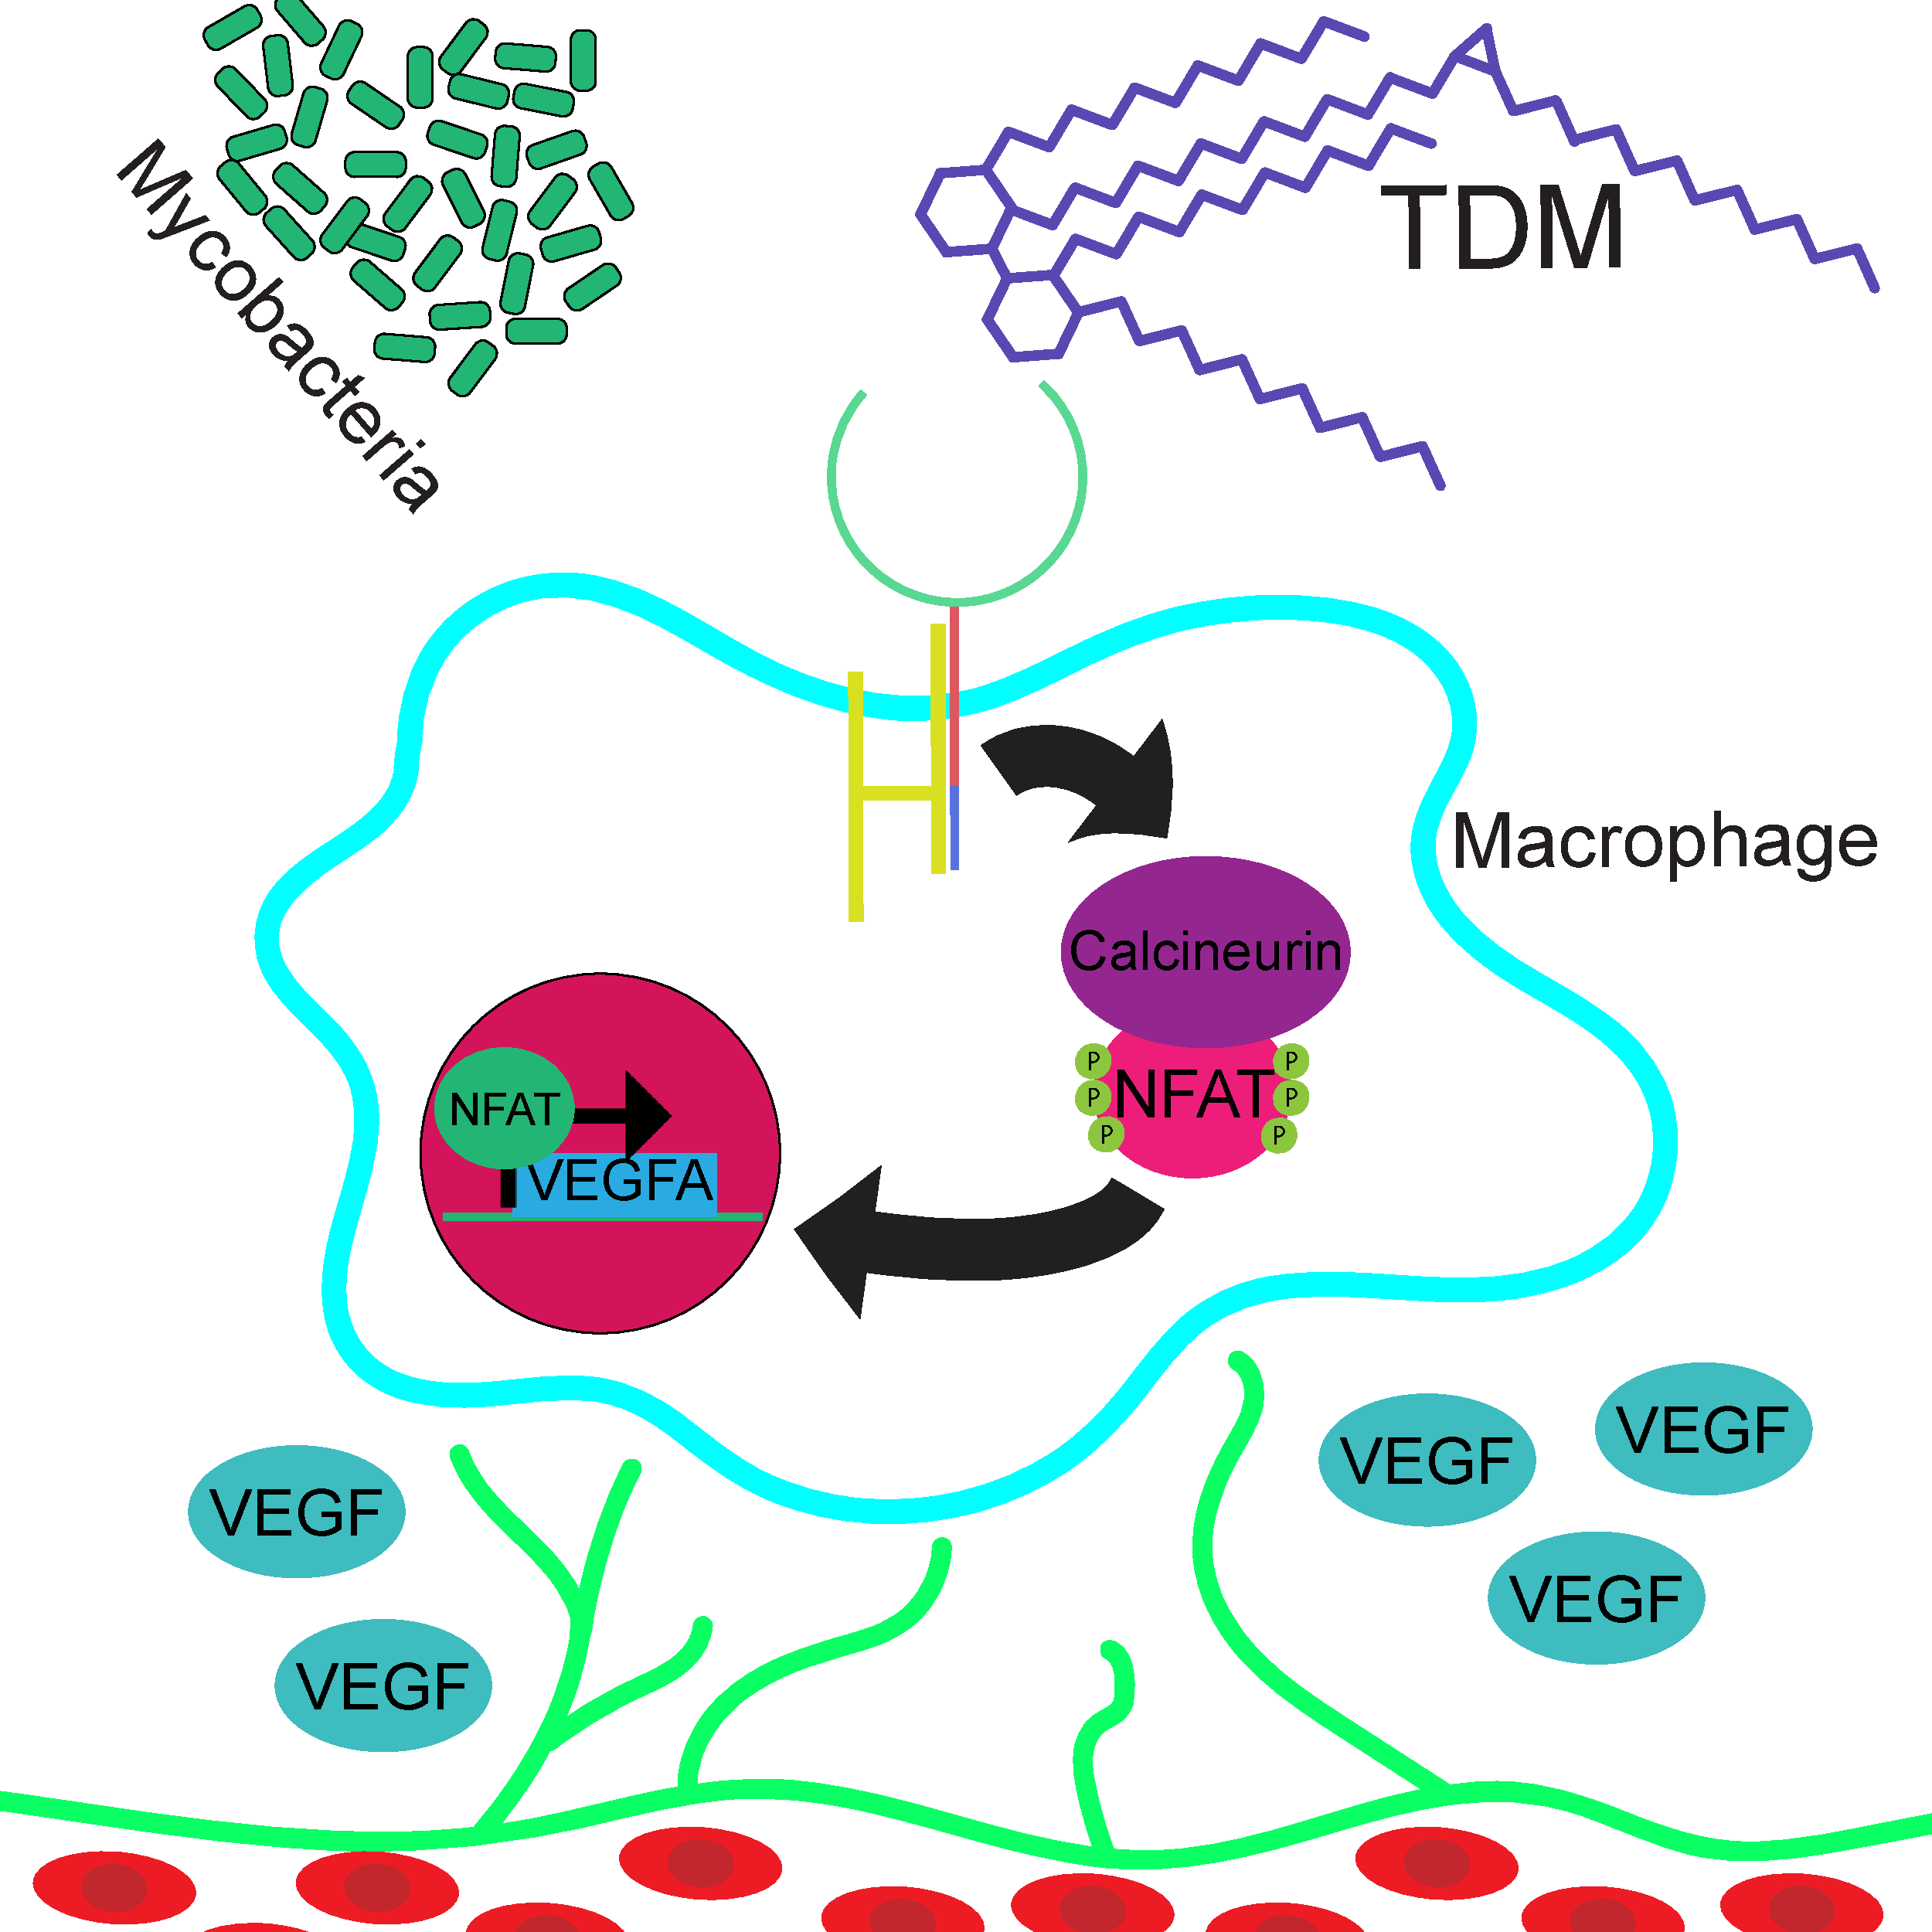
\includegraphics[width=\textwidth]{images/graphicalabstract.pdf}
\caption{This is a graphical representation of the work completed here, which found a novel role for NFAT activation downstream of macrophage\hyp{}mycobacterial surface interactions that facilitated the production and secretion of VEGFA to drive angiogenesis.}
% Provide a label so we can cross\hyp{}reference it from the tex
\label{figure:graphicalabstract}
\end{figure}

As introduced in the previous chapters, pathogenic mycobacteria manipulate the host immune response to generate a productive infection that enables them to transmit to new hosts. To do so, they must both subvert protective immune responses and agonize the pathways that provide them benefit in the way of nutrients, susceptible host cells, or routes of transmission. This necessitates the engagement of both the immune cells themselves and the surrounding stromal cells, all of which much be subverted to generate the optimal pro\hyp{}bacterial response within the limits of bacterial control of host physiology. One of the mechanisms by which this has been found to occur is through a specific modification of the specialized cell wall lipid, trehalose 6\hyp{}6'\hyp{}dimycolate (TDM). This mycobacterial glycolipid has been found to direct angiogenesis toward nascent granulomas to enhance overall bacterial burden. The present study utilizes the zebrafish\hyp{}\textit{Mycobacterium marinum} infection model to define the signaling basis of the host angiogenic response. Through intravital imaging and targeted, cell\hyp{}specific peptide\hyp{}based inhibition, we identify macrophage\hyp{}specific activation of NFAT signaling as essential to TDM\hyp{}mediated angiogenesis in vivo.  Exposure of human cells to \textit{Mycobacterium tuberculosis} results in robust induction of VEGFA that is dependent on a signaling pathway downstream of host TDM detection and culminates in NFATC2 activation. As granuloma\hyp{}associated angiogenesis is known to serve bacterial\hyp{}beneficial roles, these findings identify potential host targets to improve tuberculosis disease outcomes.

\section{Introduction}\label{pap:intro}

The host rejoinder to infection is driven by an intricately regulated, but occasionally discordant or maladaptive, immune response to pathogenic stimuli at the cell\hyp{}intrinsic, innate, and adaptive levels \citep{Iwasaki2010, Finlay2006, Haldar2015, MacMicking2004, MacMicking2012, Kim2012}. Although an inflammatory immune response is essential to host survival and pathogen killing, an overly robust response is clearly deleterious to the host, as seen in sepsis \citep{Finethy2020, Casadevall2003}. However, as we have been in previous chapters, the inflammatory response can also serve pro\hyp{}bacterial purposes, rendering the immune response impotent. The contributions of immune cells to host defense have been widely studied, but there is growing appreciation for the contributions non\hyp{}immune populations, including stromal cells and the endothelium \citep{Honan2021, Worrell2021, Amersfoort2022, Honan2021} make in shaping the host response to both acute and chronic infections \citep{Mueller2009, Randow2013, Krishnamurty2020}. Pathogens have long been known to possess sophisticated mechanisms to undermine signaling pathways in immune cells and, more recently, have been shown to manipulate development and homeostatic tissue processes to force them toward pathogen\hyp{}beneficial states \citep{Menzies1998, Guichard2013}.

\textit{Mycobacterium tuberculosis} is among history's most widespread and successful pathogens. It has evolved an array of sophisticated mechanisms that manipulate its human host to enable bacterial survival, replication, and transmission. Upon infection, \textit{M. tuberculosis} sets in motion an intricate immune response wherein innate immune cells, consisting initially of macrophages, congregate at the bacterial focus and then undergo an epithelioid transformation and interdigitate to form an encased granuloma, the hallmark feature of tuberculosis (\autoref{mamaw}), which provides both the replicative niche and the major host\hyp{}pathogen interface of tuberculosis disease \citep{Cronan2016, Pagan2018, Cronan2021}. Granuloma\hyp{}associated vasculature has long been noted in human and animal models of TB \citep{Cudkowicz1952, Russell2010} but the mechanisms of induction and precise contributions to infection are not yet fully understood (\autoref{granang}).

Many of the major pathological features of mycobacterial granulomas, including associated vascularization, are conserved from zebrafish to humans \citep{Swaim2006, Bohrer2021}. Zebrafish can be infected with a natural pathogen, \textit{Mycobacterium marinum}, which induces a robust angiogenic response during granuloma formation in both the larva and adult (\autoref{zfmm}). This process, much like that in humans, non\hyp{}human primates, and rabbits, is associated with production of a pro\hyp{}angiogenic chemokine, Vegfaa, at the site of infection \citep{Oehlers2015}. This chemokine has long been known to be a critical regulator of angiogenesis in both developmental and pathological contexts \citep{Chung2011, Leung1989, Adams2007}. Similarly, human granulomas have been shown to express VEGFA and are physically associated with blood vessels that penetrate the outer granulomatous layers \citep{Datta2015}. Subsequent work has demonstrated a role for these vessels in supporting bacterial growth and in dissemination of the bacilli from their primary site of infection \citep{Polena2016}. Additional roles for VEGFA in non\hyp{}angiogenic processes have also been noted, suggesting that angiogenic signaling cascades can also alter the biology of granuloma macrophages to exacerbate disease \citep{Harding2019}. Additional roles have been proposed for the related lymphangiogenesis \citep{Alitalo2005, Duong2012, Lerner2020}, where pharmacological blockade of these vessels of the lymphatic system also offer host\hyp{}protective benefits \citep{Harding2015}. Recent profiling of human and non\hyp{}human primate granulomas have confirmed the presence of aberrant vasculature associated with \textit{M. tuberculosis} granulomas \citep{Gideon2022, McCaffrey2022, Cronan2021}, although more complete characterization of the endothelium itself is lacking.

Pathogenic mycobacteria have evolved specialized mechanisms to promote and accelerate angiogenesis and modulate other aspects of endothelial biology \citep{Oehlers2017}. Notably, the extensively modified and essential outer cell envelope component trehalose 6\hyp{}6'\hyp{}dimycolate (TDM) is cis\hyp{}cyclopropanated by the enzyme PcaA \citep{Glickman2000, Rao2005}. Mutation of pcaA results in a reduction in granuloma angiogenesis and concomitant reduction in bacterial burden; correspondingly, cyclopropanated TDM alone is sufficient to induce host angiogenesis \citep{Saita2000, Sakaguchi2000, Walton2018} (\autoref{granang}). As \textit{pcaA}\hyp{}dependent vascularization supports bacterial growth, factors driving angiogenesis represent potential sites of therapeutic intervention yet the signals that mediate this host process remain unclear.

\begin{figure}
\centering
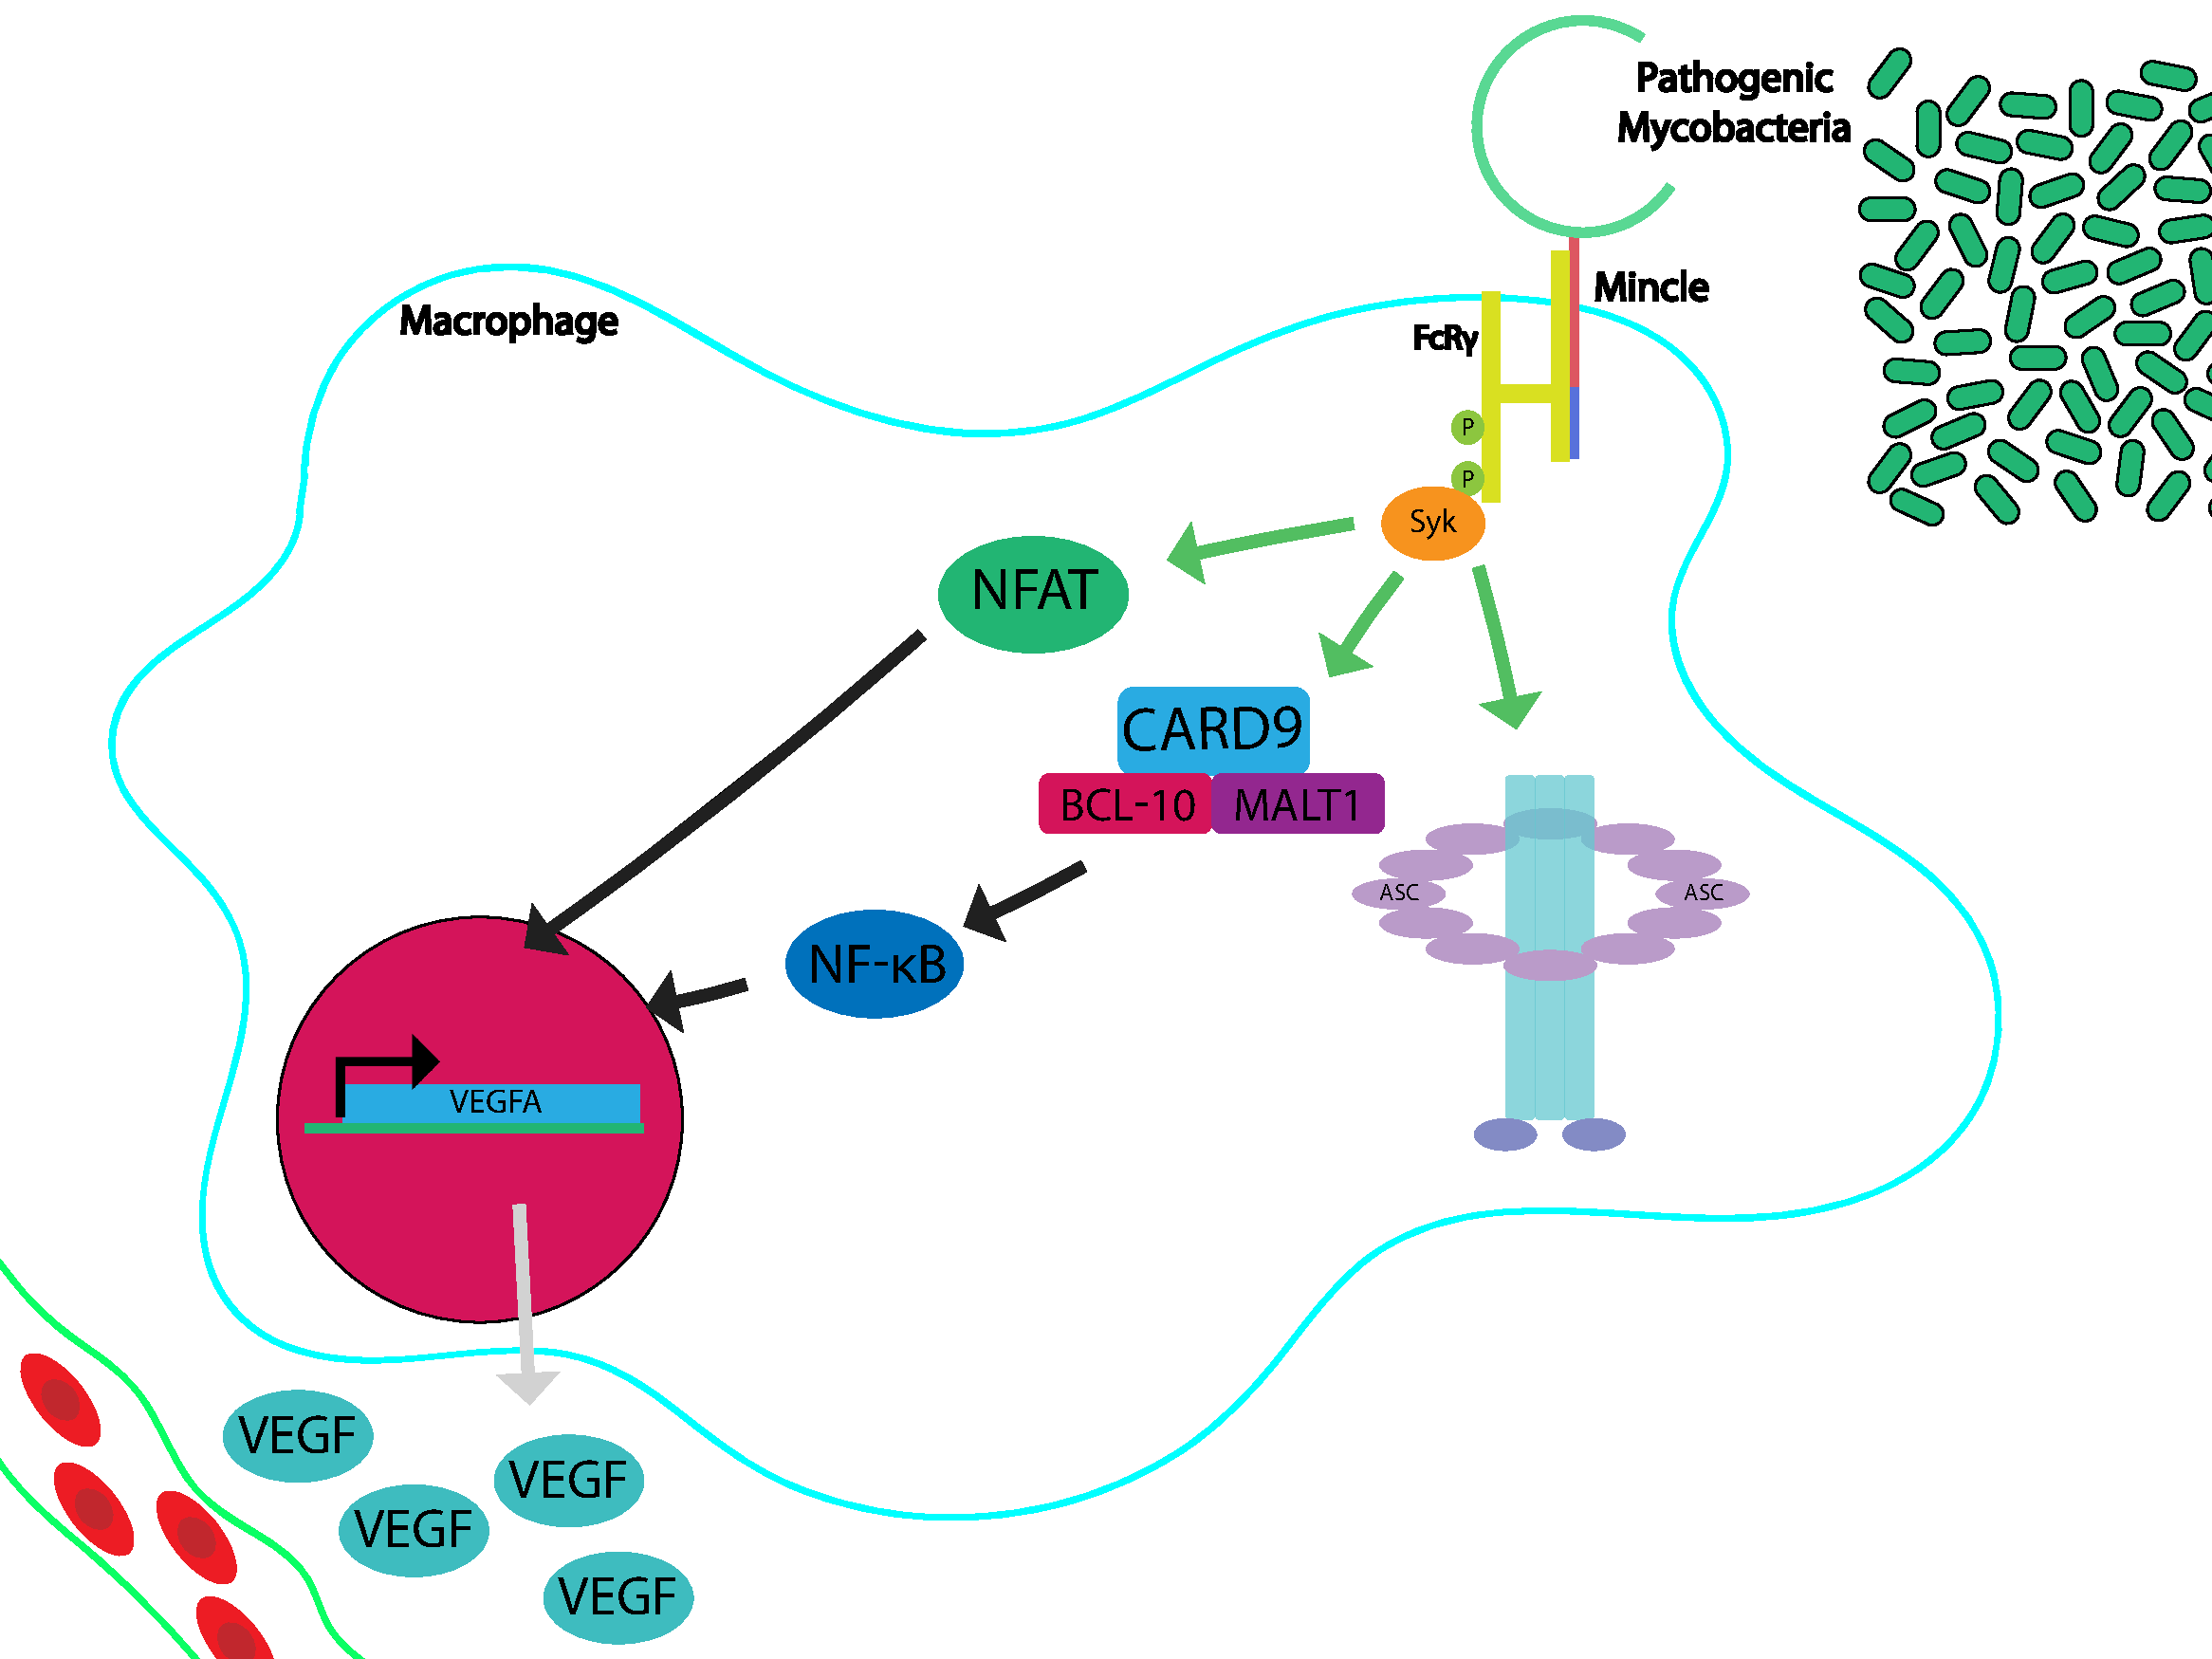
\includegraphics[width=\textwidth]{images/intro_schematic.pdf}
\caption{The central hypothesis of this work is that a discrete pathway downstream of C\hyp{}type lectin receptor activation is mediating the induction of VEGFA within macrophages to drive angiogenesis during mycobacterial infections. This schematic displays the hypothesized pathway options that could be playing these roles: CARD9, NFAT, or inflammasome activation. This work sought to dissect these possibilities to better understand the mechanism of angiogenesis during tuberculosis infection.}
% Provide a label so we can cross\hyp{}reference it from the tex
\label{figure:beginschematic}
\end{figure}

TDM is an extraordinarily long\hyp{}chain, hydrophobic (C\textsubscript{60}\hyp{}C\textsubscript{100}) glycolipid \citep{Noll1956a, Noll1956b, Hunter2006a, Behling1993} that has been shown to be detected in cell culture and murine models by host C\hyp{}type lectin receptors, most notably MCL (CLEC4D) and MINCLE (CLEC4E), as well as by Toll\hyp{}like receptor 2 (TLR2), CD14, and MARCO \citep{Bowdish2009, Matsunaga2009, Miyake2013, Ishikawa2009} (see also \autoref{tdmreceptor}). Canonically, C\hyp{}type lectin signaling is transmitted through a CARD9\hyp{}NF\hyp{}$\upkappa$B signaling pathway that results in the transcription and production of TNF\hyp{}$\upalpha$, IL\hyp{}1$\upbeta$, IL\hyp{}6 and other cytokines \citep{Yamasaki2008, Goodridge2009, LobatoPascual2013, Zhao2014, Deerhake2021} (\autoref{clr:nfat}, \autoref{NFAT}). However, beyond CARD9, a number of other downstream signaling pathways are engaged by C\hyp{}type lectin activation and likely control discrete aspects of signaling \citep{Goodridge2007, Deerhake2021}.

Here, we synthesize findings from zebrafish and cell culture models to define the \textit{in vivo} angiogenic response induced by pathogenic mycobacteria. Contrary to classical models of C\hyp{}type lectin signaling, we find that cis\hyp{}cyclopropanated TDM exerts its pro\hyp{}angiogenic effects through an alternative NFAT\hyp{}driven pathway rather than canonical CARD9\hyp{}NF\hyp{}$\upkappa$B signaling. We use peptide\hyp{}mediated, cell\hyp{}specific inhibition of NFAT to demonstrate that both early and mature granuloma angiogenesis are dependent upon macrophage\hyp{}NFAT signaling. We identify \textit{NFATC2} as the predominant isoform mediating \textit{VEGFA} induction and angiogenesis \textit{in vitro} and \textit{in vivo}. These findings define the basis of granuloma\hyp{}associated angiogenesis during pathogenic mycobacterial infections and suggest new targets for host\hyp{}directed therapeutic interventions during tuberculosis.

\section{Results}

\subsection{Macrophage Induction of \textit{vegfaa} and Angiogenesis during Mycobacterial Infection}

\begin{figure}
\centering
\includegraphics[width=\textwidth]{images/angexample.pdf}
\caption{Pictorial representation of the site of infection and angiogenic outcomes from infection. After injection into a peri\hyp{}notochordal space along the trunk of the fish, the bacteria replicate and blood vessels grow toward the site of infection, as compared to the uninfected reference.}
% Provide a label so we can cross\hyp{}reference it from the tex
\label{figure:angexample}

\end{figure}

Injection of live \textit{Mycobacterium marinum} into the dorsal trunk of the zebrafish larva is sufficient to induce a robust angiogenic response adjacent to nascent granulomas in a macrophage\hyp{}dependent manner \citep{Oehlers2015} (\autoref{figure:angexample}). The stereotyped vasculature along this region of the larva allows facile quantitation of neovascularization during and after granuloma formation or other insult \citep{Lawson2002, Jin2005, Gore2012, Matsuoka2018} (\autoref{zfvasc}). We demonstrated previously that cis\hyp{}cyclopropanated trehalose 6\hyp{}6'\hyp{}dimycolate (TDM) is required for the induction of \textit{vegfaa} and angiogenesis at the site of infection. Furthermore, we found that genetic blockade of Vegfaa signaling was sufficient to abolish angiogenesis during infection with wild\hyp{}type mycobacteria \citep{Walton2018}. Taken together, these findings suggest that the failure to induce \textit{vegfaa} is a primary contributor to the loss of angiogenesis in \textit{pcaA}\hyp{}deficient granulomas.

\begin{figure}
\centering
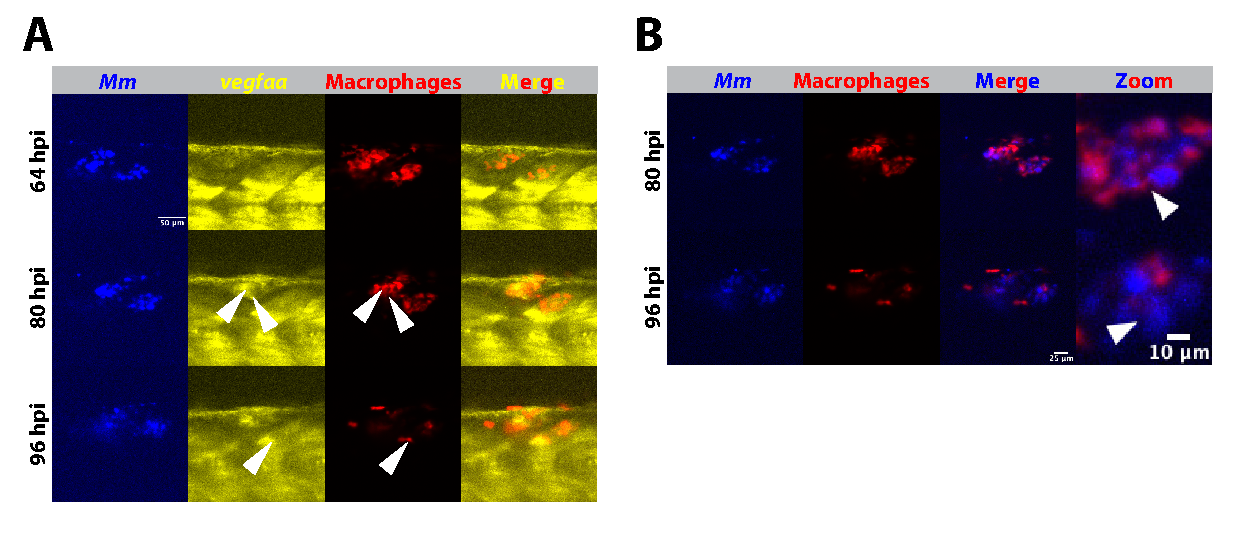
\includegraphics[width=\textwidth]{images/extracellularvegfa.pdf}
\caption{Around 60 hours post infection, macrophages interacting with the extracellular bacteria at the site of infection begin to express \textit{vegfaa}, as reported by the \textit{vegfaa}:\textit{eGFP\textsuperscript{pd260}} transgene. In (A), a time series can be seen showing \textit{vegfaa}\hyp{}expressing macrophages and in (B), macrophages can be seen engaging with what appears to be extracellular bacteria that has accumulated over the course of the infection.}
% Provide a label so we can cross\hyp{}reference it from the tex
\label{figure:ecvegfa}

\end{figure}

To study this phenomenon further, we began by examining the kinetics of \textit{vegfaa} induction to identify the cellular source of Vegfaa during granuloma formation. To test whether macrophages were playing this role, we developed a macrophage\hyp{}specific reporter using the previously described \textit{acod1} promoter (also known as \textit{irg1}), Tg(\textit{irg1}:\textit{tdTomato\textsuperscript{xt40}}) (from here, \textit{irg1}:\textit{tdTomato}). \textit{irg1} has been found to be expressed specifically in zebrafish macrophages and is upregulated during infection \citep{Sanderson2015, Kwon2022}. We then crossed this line with the \textit{vegfaa} reporter line TgBAC(\textit{vegfaa}:\textit{eGFP\textsuperscript{pd260}}) (\textit{vegfaa}:\textit{eGFP} throughout) \citep{Karra2018} and infected double transgenic \textit{irg1}:\textit{tdTomato}; \textit{vegfaa}:\textit{eGFP} progeny with \textit{M. marinum} expressing eBFP2 (\textit{Mm}\hyp{}eBFP2) to simultaneously visualize bacteria, macrophage localization, and \textit{vegfaa} production \textit{in vivo} \citep{Takaki2013}.

\begin{figure}
\centering
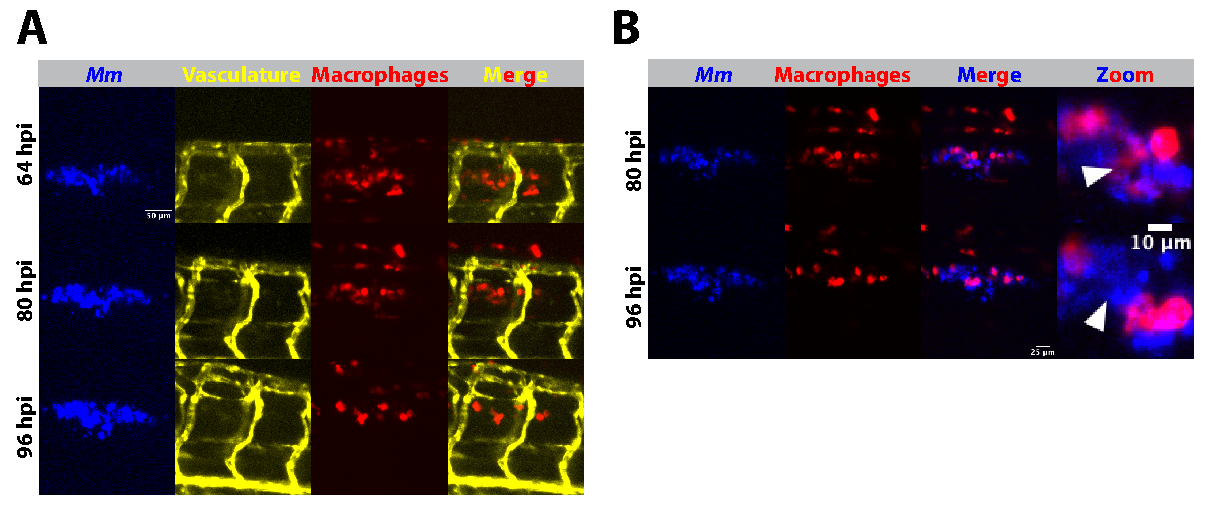
\includegraphics[width=\textwidth]{images/extracellularflk1.pdf}
\caption{At later time points, after \textit{vegfaa} induction, blood vessels proliferate and begin to grow toward the site of infection in association with nearby macrophages. (A) shows this process occurring over the time period studied and culminating in a new vessel nearly spanning the intersomitic vasculature. (B) displays the accumulation of extracellular bacteria and macrophage killing over this time period.}
% Provide a label so we can cross\hyp{}reference it from the tex
\label{figure:ecflk1}

\end{figure}

We began imaging at a time point that preceded robust induction of \textit{vegfaa}:\textit{eGFP} but would allow us to capture the maximum time span of these events. We observed an increase in \textit{vegfaa} reporter signal over time that appeared largely localized to macrophages (\autoref{figure:ecvegfa}A). We observed that bacteria initially grew primarily intracellularly within individual macrophages at 36 hours post infection but began to grow in characteristic extracellular cords by approximately 84 hours post infection with little to no intracellular containment at this site by 96 hours post infection (\autoref{figure:ecvegfa}B). The increase in extracellular growth coincided with the induction of eGFP signal in macrophages at ~64 hours (\autoref{figure:ecvegfa}A), suggesting that, at low overall burden, intracellular detection is unable to induce \textit{vegfaa} expression while extracellular engagement correlates with \textit{vegfaa} expression during early stages of granuloma formation (\autoref{figure:ecvegfa}). 

We next visualized the production of angiogenic vessels throughout infection in parallel to our characterization of \textit{vegfaa} induction. Due to an inability to separate discrete emission wavelengths using two GFP reporter lines, we were unable to examine all four components (bacteria, \textit{vegfaa} induction, macrophages, and vasculature) simultaneously. To relate this process directly to the angiogenesis observed in mycobacterial granulomas, we crossed the \textit{irg1}:\textit{tdTomato} macrophage reporter to the Tg(\textit{kdrl}:\textit{eGFP\textsuperscript{s843}}) (from here, \textit{kdrl}:\textit{eGFP}) line, which labels vascular endothelium (\textit{irg1}:\textit{tdTomato}; \textit{kdrl}:\textit{eGFP}) \citep{Jin2005}. Under the same conditions and burden at which we infected the \textit{vegfaa} and macrophage dual reporter line, we observed robust vascularization at approximately 96 hours post\hyp{}infection, subsequent to initial granuloma formation and \textit{vegfaa} induction (\autoref{figure:ecflk1}A, B). 

\subsection{Genetic \textit{card9} Deficiency Does Not Compromise Angiogenesis During Mycobacterial Infection}

\begin{figure}
\centering
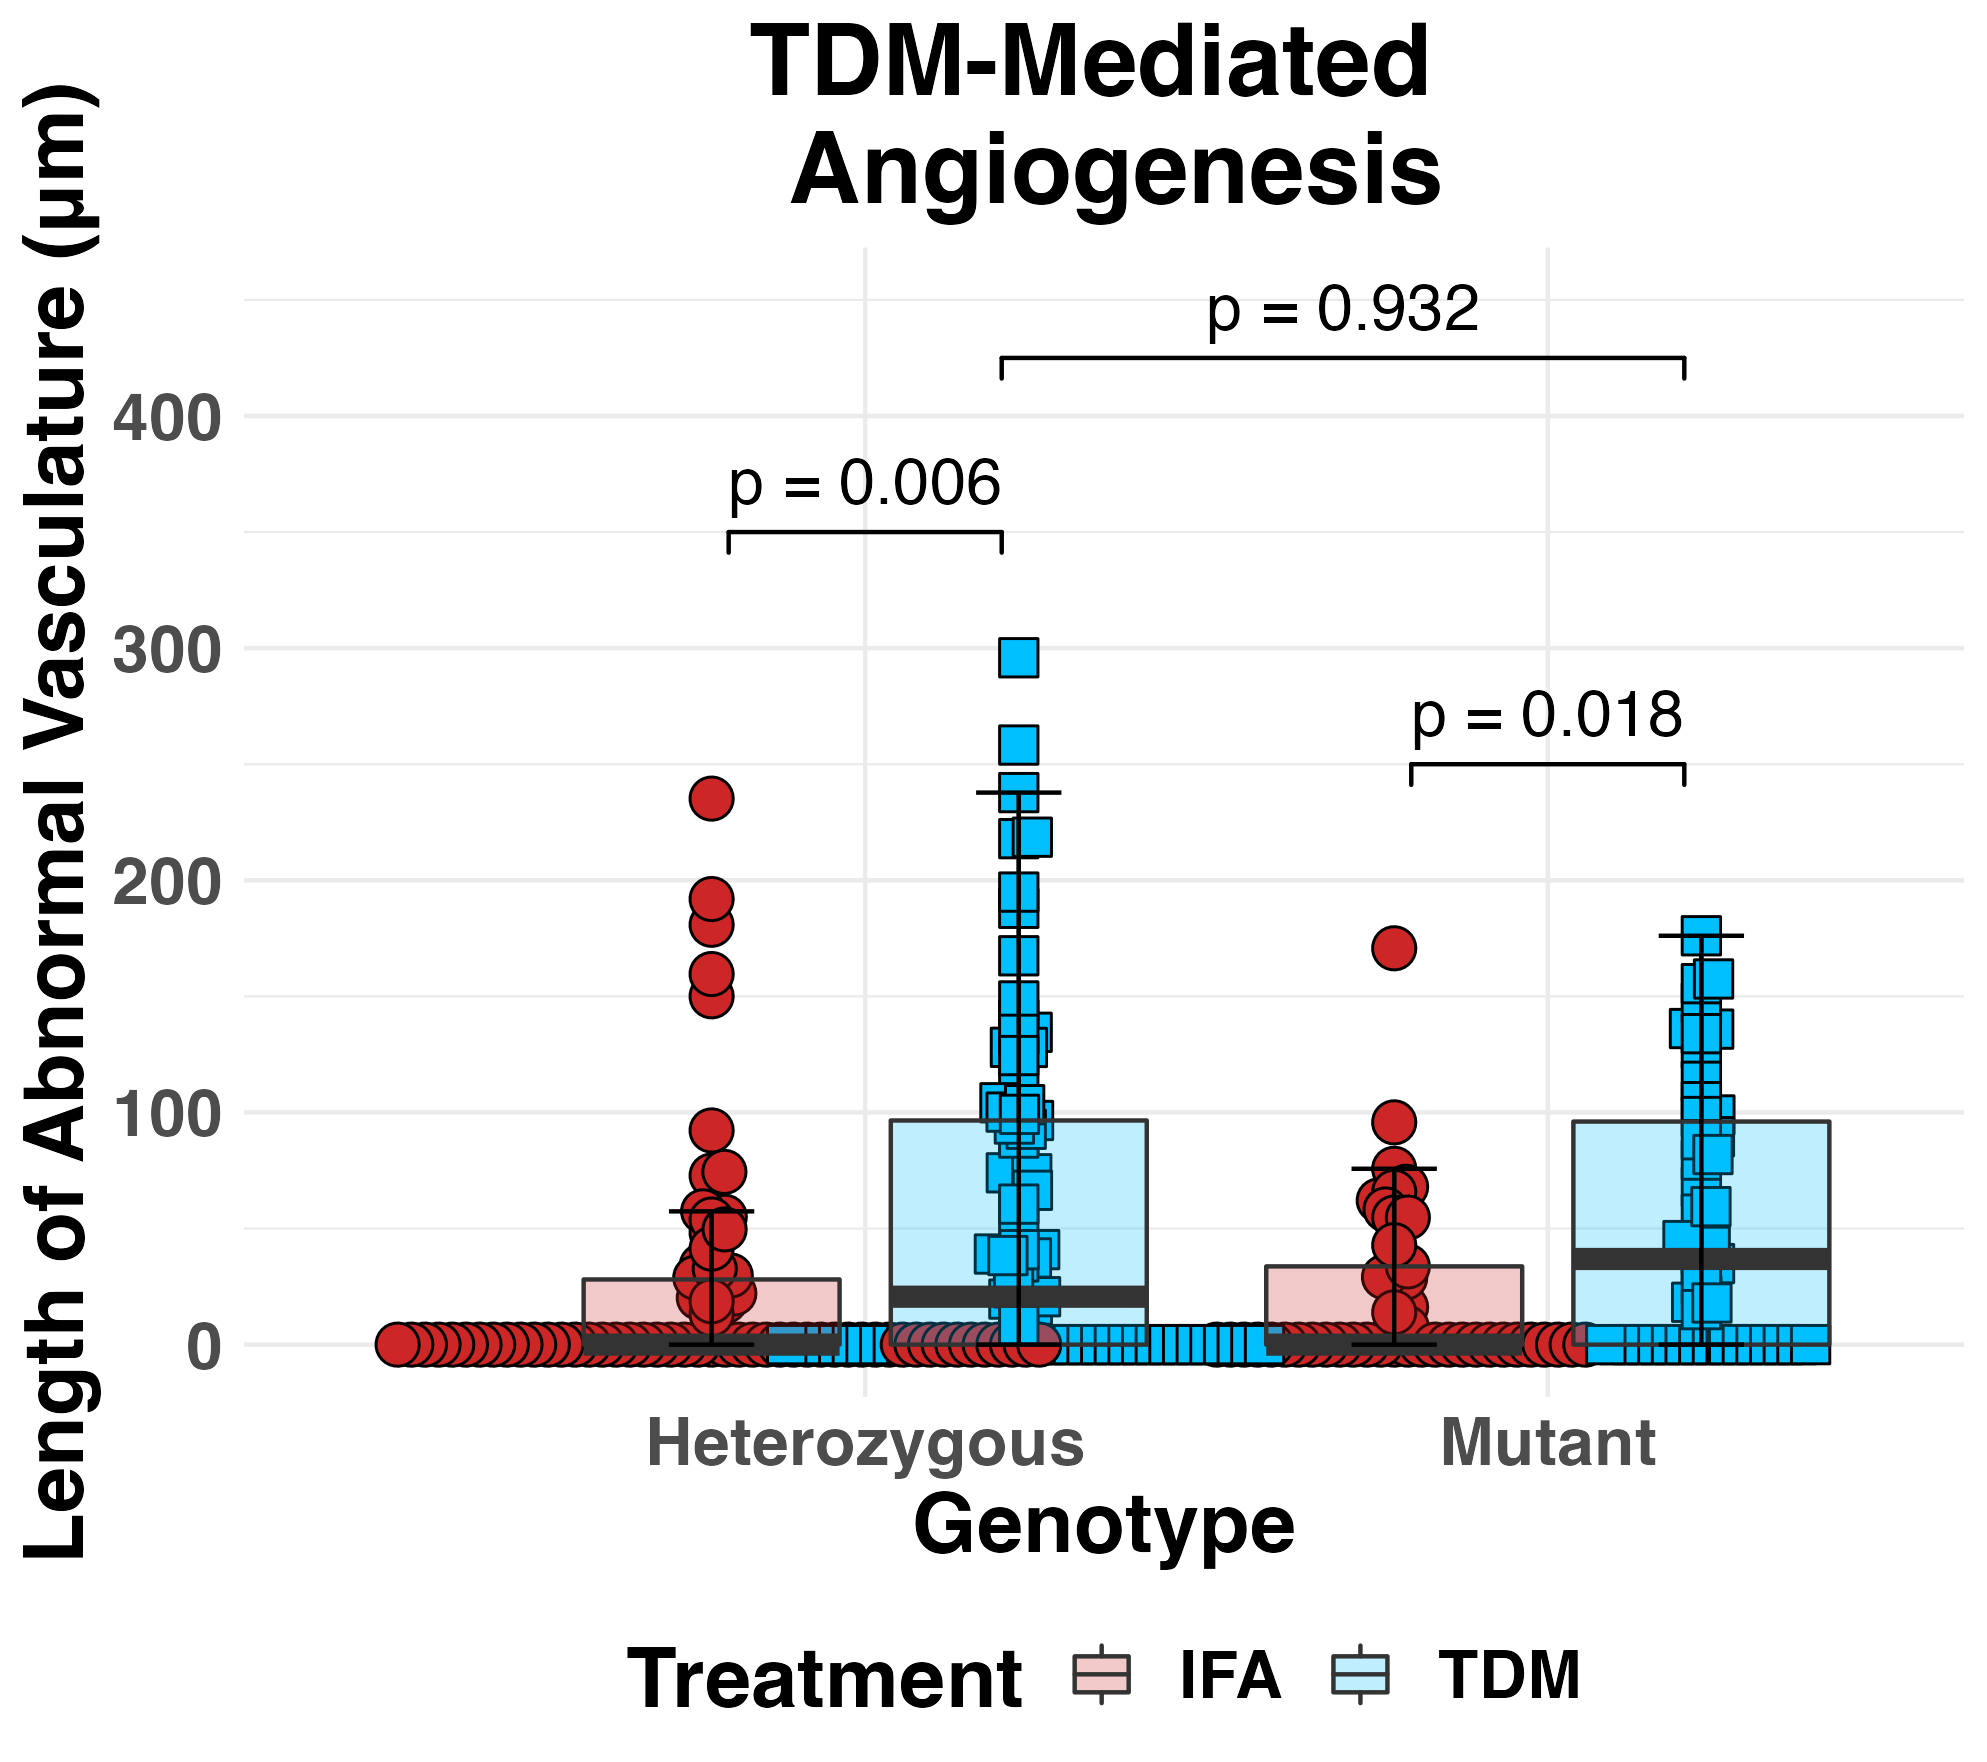
\includegraphics[height=3in]{images/JB96_myd88_TDM_103022.png}
\caption{\textit{myd88} is dispensable for angiogenesis during infection, suggesting a TLR\hyp{} and IL\hyp{}1R\hyp{}independent signaling pathway is necessary for inducing angiogenesis downstream of TDM detection. Larval zebrafish were injected with IFA or TDM, imaged and quantitated, and then matched to genotype. Adapted from personal contributions to \citet{Walton2018}.}
% Provide a label so we can cross\hyp{}reference it from the tex
\label{figure:myd88}

\end{figure}

Given these observations suggesting that macrophages engaging extracellular bacteria are an important source of \textit{vegfaa} expression, we interrogated pattern recognition receptor (PRR) signaling pathways that had been implicated in host responses to TDM, a major external component of the mycobacterial cell envelope. We had previously found that \textit{myd88} was dispensable for the induction of angiogenesis in response to TDM \textit{in vivo} (\autoref{figure:myd88}) \citep{Bowdish2009, Walton2018}. This suggested that the described TLR2\hyp{} or IL\hyp{}1R\hyp{}mediated responses that function downstream of TDM detection in some contexts were unlikely to be required for this process\footnote{This could not, however, rule out any potential role for CD14\hyp{}mediated signaling independent of TLR2. One issue is that the zebrafish do not have an identified CD14 homolog, but additional data clarifies things somewhat.}. Rather, we found that the Fc$\upgamma$R homologs in zebrafish, \textit{fcer1g} and \textit{fcer1gl}, are required for the full angiogenic response to TDM \citep{Walton2018}, implicating C\hyp{}type lectin receptors signaling in mediating this response \citep{Richardson2014, Zhao2014}.

\begin{figure}
\centering
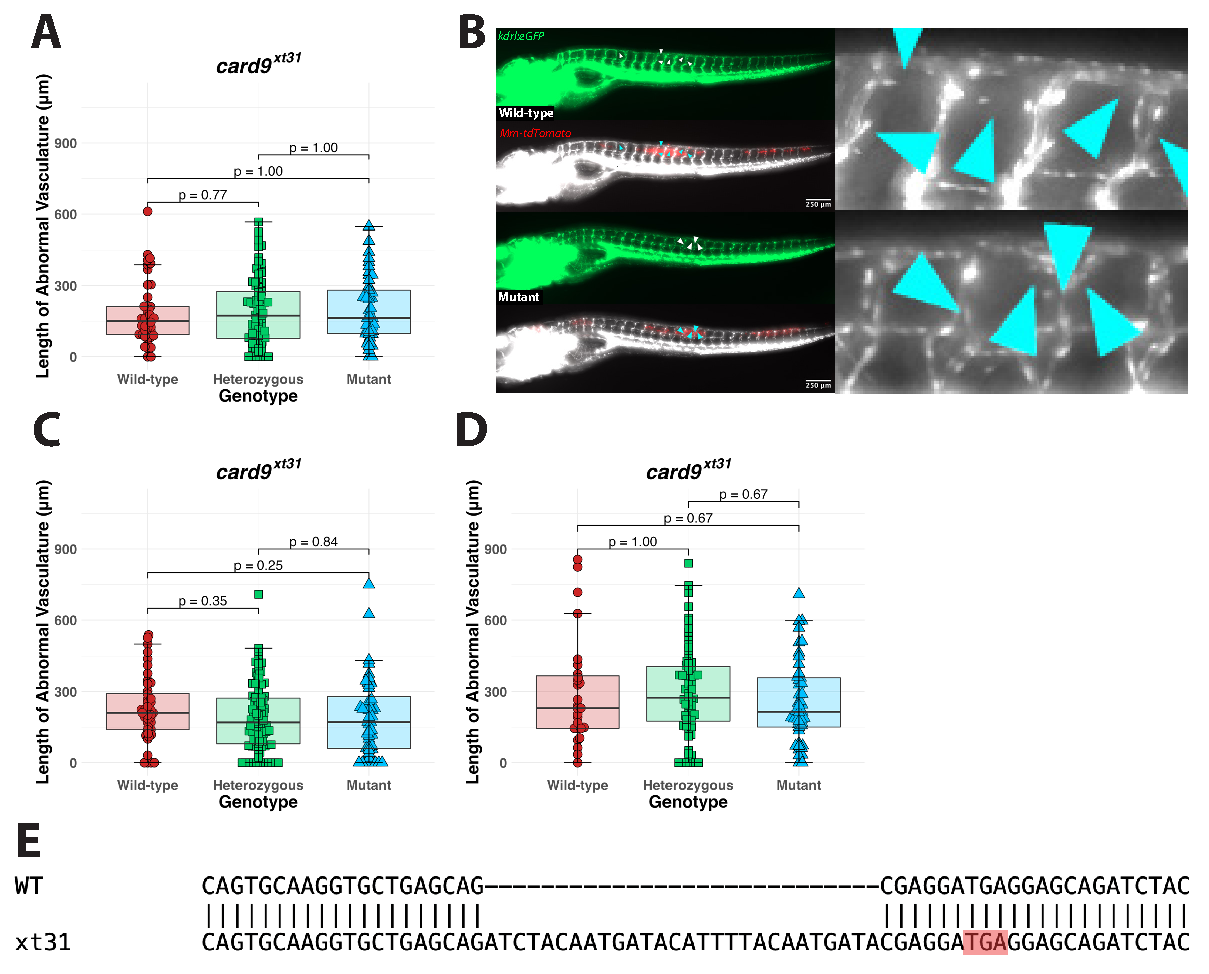
\includegraphics[width=\textwidth]{images/card9.pdf}
\caption{\textit{card9}, the canonical downstream adaptor from C\hyp{}type lectin signaling, is not required for angiogenesis during mycobacterial infection. (A), (C), and (D) show three replicates of this experiment from genotype\hyp{}blind experiments. (B) shows a representative example of the effect seen, where no differences can be ascertained between genotypes. (E) displays the 28 base pair insertion generated, with the new early stop codon highlighted in red.}
% Provide a label so we can cross\hyp{}reference it from the tex
\label{figure:card9}
\end{figure}

As many of the downstream activities of C\hyp{}type lectin receptors have been ascribed to the activation of CARD9\hyp{}NF\hyp{}$\upkappa$B signaling \citep{Goodridge2009, LobatoPascual2013, Zhao2014, Williams2017, Deerhake2021}, we assessed what role this pathway might play in angiogenesis during mycobacterial infection. We developed a \textit{card9} knockout zebrafish line using CRISPR/Cas9 that carries a 28 bp insertion, resulting in an early stop after 59 amino acids (\textit{card9\textsuperscript{xt31}}) (\autoref{figure:card9}E). We then assayed these animals in the \textit{kdrl}:\textit{eGFP} transgenic background by incrossing \textit{kdrl}:\textit{eGFP}; \textit{card9\textsuperscript{xt31/+}} animals and infecting the resulting offspring with tdTomato\hyp{}fluorescent \textit{M. marinum} (\textit{Mm}\hyp{}tdTomato) at 2 days post fertilization \citep{Jin2005, Oehlers2015}(\autoref{figure:card9}A, B). We quantitated the resulting aberrant vasculature at 4 days post\hyp{}infection under genotypic blinding and post hoc matched these measurements to genotype. To my surprise, there were no significant differences between the three genotypes across three independent replicates (\autoref{figure:card9}A, C, D), suggesting either redundancy between multiple established pathways or the existence of an alternative pathway downstream of TDM detection that was \textit{fcer1g}/\textit{fcer1gl}\hyp{}dependent, but independent of both \textit{myd88} and \textit{card9}. 

As C\hyp{}lectin receptors are also known to activate inflammasome formation, we sought to assess whether non\hyp{}canonical\footnote{Based on the \textit{myd88} data, we already knew at this point that IL-1$\upbeta$ signaling was dispensable for angiogenesis as IL-1R-dependent responses rely on MYD88 for intracellular signal transduction.} functions of the inflammasome may be required for the angiogenic response. We thus utilized an \textit{asc} knockout line (\textit{asc\textsuperscript{w216}}, which abolishes inflammasome nucleation and subsequent processing of IL-1$\upbeta$, IL-18\footnote{Zebrafish do not have an annotated IL-18, although they may have some analogous that has not yet been identified.}, and Gasdermin D processing\footnote{Given the known roles for adenosine receptor signaling in inducing angiogenesis, it was possible that inflammasome-mediated cell death pathways could be indirectly responsible for inducing angiogenesis, although this does not appear to be the case in this instance \citep{Clark2007, Montesinos2002, Dusseau1986, Auchampach2007}.}. Similar to previous assays, we incrossed heterozygotes of \textit{asc\textsuperscript{w216}} in the \textit{kdrl}:\textit{eGFP} background (\textit{kdrl}:\textit{eGFP}; \textit{asc\textsuperscript{w216}}) and injected the resulting offspring with TDM or the IFA vehicle. We found that \textit{asc\textsuperscript{w216/w216}} zebrafish were competent for angiogenesis in response to TDM (\autoref{figure:asc}), suggesting that this pathway was also dispensable for angiogenesis and narrowing our focus onto the NFAT signaling pathway.

\begin{figure}
\centering
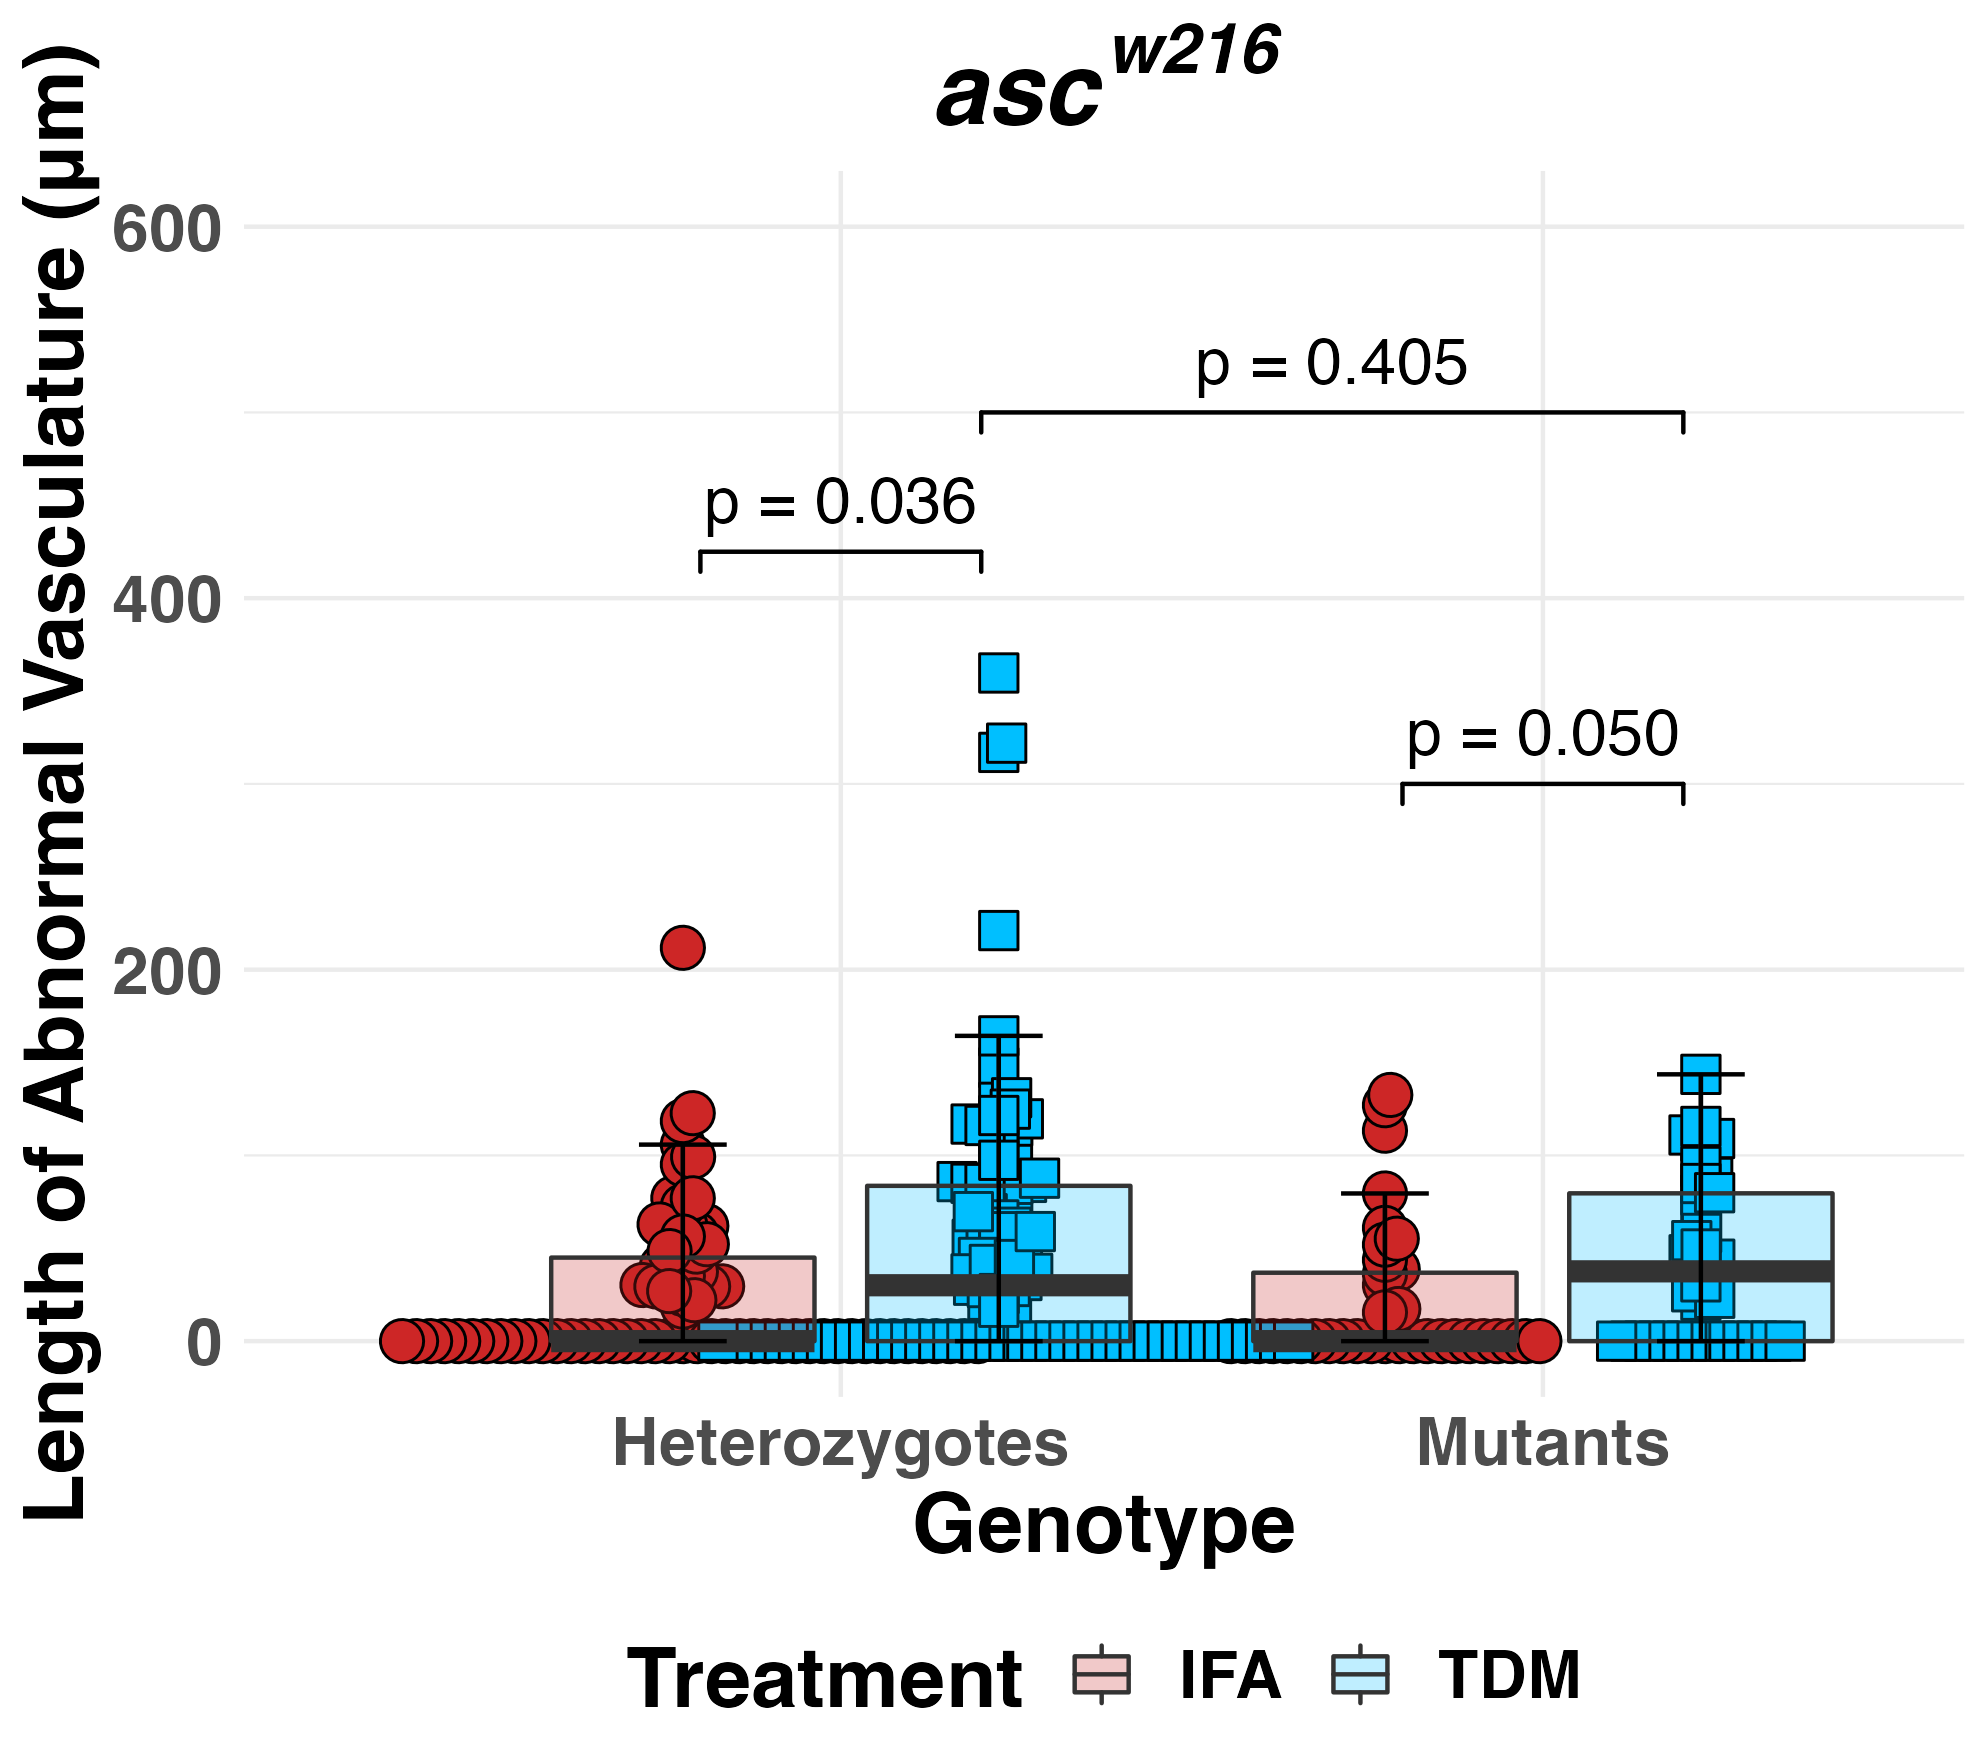
\includegraphics[width=\textwidth]{images/asc_tdm_110922.png}
\caption{\textit{asc}, the critical downstream adaptor protein for the formation of the inflammasome, is not required for angiogenesis in response to purified mycobacterial TDM.}
% Provide a label so we can cross\hyp{}reference it from the tex
\label{figure:asc}
\end{figure}

\subsection{Pharmacological Inhibition of NFAT Activation Limits Angiogenesis in Response to Mycobacteria and TDM}

\begin{figure}
\centering
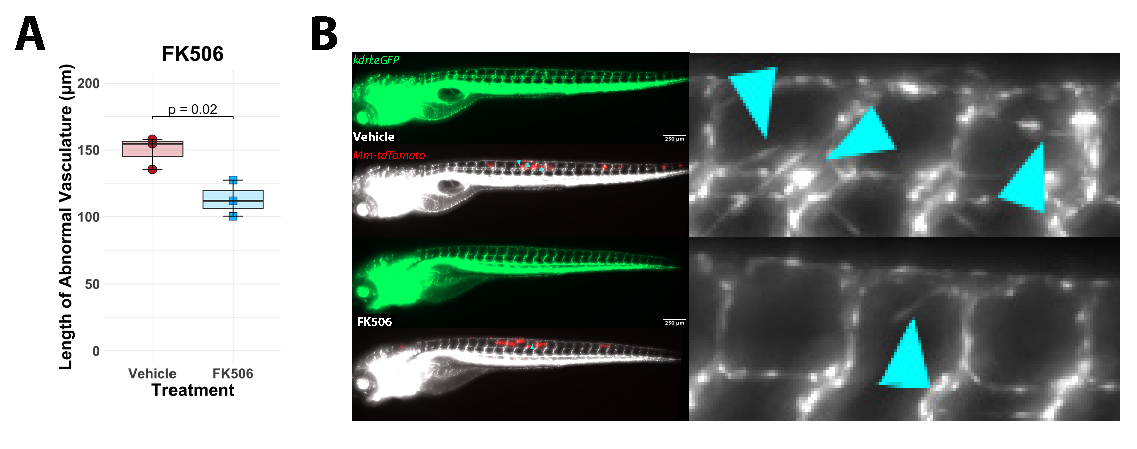
\includegraphics[width=\textwidth]{images/fk506inf.pdf}
\caption{Treatment of infected larval zebrafish with the calcineurin\hyp{}NFAT inhibitor FK506 at 125nM results in a reduction in infection\hyp{}induced angiogenesis, suggesting a role for this pathway in inducing angiogenesis during infection.}
% Provide a label so we can cross\hyp{}reference it from the tex
\label{figure:fk506inf}
\end{figure}

Although many of the physiological consequences of C\hyp{}type lectin receptor induction are often ascribed to CARD9\hyp{}NF\hyp{}$\upkappa$B signaling, this PRR class is also known to activate a distinct transcription factor family with known roles in immunity --€“ the nuclear factor of activated T cells, or NFAT \citep{Goodridge2007, Deerhake2021}. This calcium\hyp{}responsive transcription factor pathway is best described in its role regulating T cell biology, but there are numerous reports describing various roles for the members of this pathway in other cell types, including macrophages (see \autoref{NFAT}) \citep{Symes1998, Jones2000, Crabtree2002, Horsley2002, Elloumi2012}. Given that there are four mammalian members of this pathway and six zebrafish homologs with potentially overlapping functions, we began with a pharmacological approach to globally inhibit NFAT signaling through all six zebrafish isoforms. Although this comes with caveats with specificity -- as described in \autoref{nfatc1}, NFATC1 has important roles in angiogenesis within the endothelium -- it offers an opportunity to assess the general roles of this pathway as a first\hyp{}pass approach. 

\begin{figure}
\centering
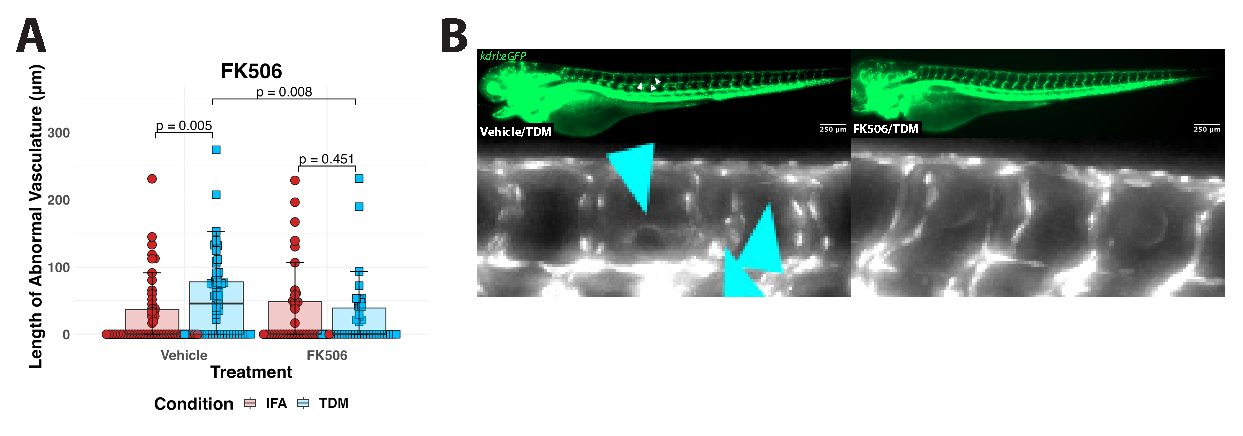
\includegraphics[width=\textwidth]{images/fk506tdm.pdf}
\caption{Treatment of infected larval zebrafish with the calcineurin\hyp{}NFAT inhibitor FK506 at 125nM results in a reduction in TDM\hyp{}induced angiogenesis, suggesting a role for NFAT signaling in inducing TDM\hyp{}dependent pro\hyp{}angiogenic signaling.}
% Provide a label so we can cross\hyp{}reference it from the tex
\label{figure:fk506tdm}
\end{figure}

We first infected 2 days post fertilization \textit{kdrl}:\textit{eGFP} larval zebrafish with \textit{Mm}\hyp{}tdTomato in the trunk and treated them with 125 nM FK506, a clinically utilized calcineurin inhibitor that blocks NFAT activation, for the duration of the experiment \citep{Ellis1995} (\autoref{tacrolimus}). This minimal dose of FK506 was chosen due to developmental toxicities observed at higher doses in my hands and is in line with the dosage used by others \citep{Kujawski2014}. We imaged the fish at 4 days post infection and quantitated the degree of vasculature induced in the presence and absence of inhibitor under computational blinding. Even with at this low dose of FK506, we noted a small, but statistically significant reduction in the mean degree of neovascularization at this time point, consistent with a role for NFAT in controlling angiogenesis in response to \textit{M. marinum} infection (\autoref{figure:fk506inf}A, B) \citep{Kujawski2014}. To ask whether this effect was specific to recognition of TDM, we injected purified TDM or vehicle (incomplete Freund's adjuvant; IFA) alone into the trunks of 2 days post fertilization larvae. Treatment with FK506 resulted in a statistically significant reduction in the degree of angiogenesis induced at 2 days post injection (\autoref{figure:fk506tdm}A, B), suggesting that this pathway was specifically relevant to TDM\hyp{}dependent angiogenesis.

\subsection{The Isoform \textit{nfatc2a} is Specifically Required for Angiogenesis During Infection}

\begin{figure}
\centering
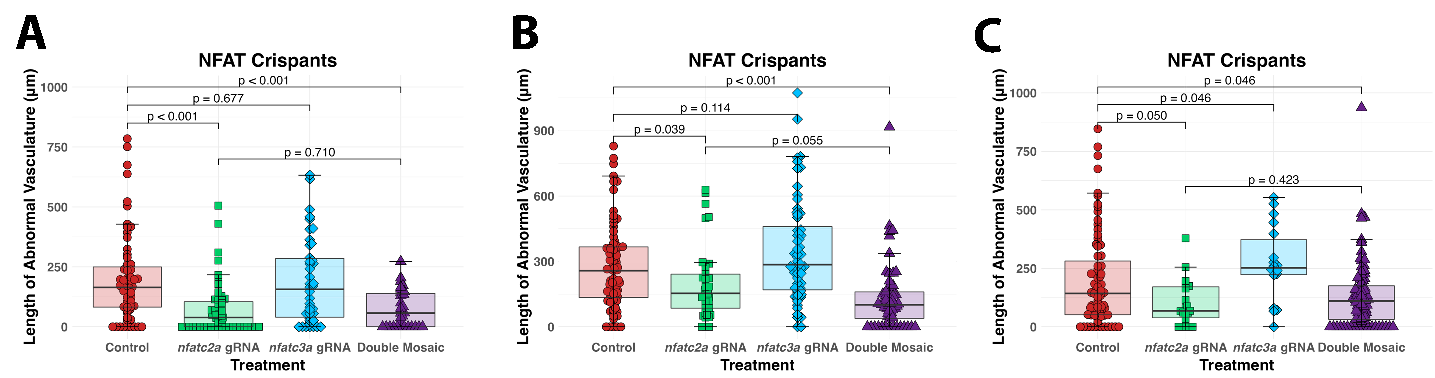
\includegraphics[width=\textwidth]{images/mosaicnfatc3a.pdf}
\caption{Assays in mosaic, CRISPR/Cas9 RNP\hyp{}injected larval zebrafish suggested that \textit{nfatc3a} was dispensable for the induction of angiogenesis during infection. Panels (A), (B), (C) show the results of three replicates of these mosaic injections. (D) shows the results of the same assay in a stable knockout background of \textit{nfatc3a}, confirming the preliminary results from the mosaic assay. (E) shows the nature of the mutation in \textit{nfatc3a\textsuperscript{xt59}}.}
% Provide a label so we can cross\hyp{}reference it from the tex
\label{figure:mosaic}
\end{figure}

Combining our observations on the correspondence of granuloma formation and the induction of \textit{vegfaa} with our data implicating the NFAT pathway, we sought to identify NFAT isoforms that were enriched in granuloma macrophage populations. Aside from investigations made into \textit{nfatc1}, which is restricted to the endocardium, lymphatic vessels, and the notochord during much of zebrafish development (see \autoref{nfatc1}) \citep{Pestel2016, Shin2019, Bagwell2020}, little is known of the expression patterns of these genes in zebrafish\footnote{As mentioned previously in \autoref{nfatc4}, the NFATC4 isoform is thought to not be expressed in the hematopoietic compartment, an observation backed up by some more recent data as well \citep{Peuker2022}.}, especially in the context of infection. We first made use of published scRNA\hyp{}seq datasets from mycobacterial granulomas in zebrafish and non\hyp{}human primates for \textit{nfat} transcripts that were robustly expressed in granuloma macrophages at the population level and identified both zebrafish \textit{nfatc2a} and \textit{nfatc3a} as plausible candidates \citep{Cronan2021, Gideon2022}.

To examine potential roles for \textit{nfatc2a} and \textit{nfatc3a} in granuloma\hyp{}associated angiogenesis in vivo, we first screened F\textsubscript{0} CRISPR\hyp{}injected mosaic knockouts (``crispants'') to rapidly evaluate these candidate genes (\autoref{crispants}). Using this approach, similar to that used previously by other groups, we assessed the relative roles of these two isoforms individually and in tandem, measuring the angiogenic response to mycobacterial infection in the \textit{kdrl}:\textit{eGFP} background \citep{Jao2013, Hoshijima2016, Wu2018, Hoshijima2019, Kroll2021}. We found that \textit{nfatc2a} inhibition resulted in a $\sim$50\hyp{}80\% reduction in angiogenesis (\autoref{figure:mosaic}A\hyp{}C). In contrast, \textit{nfatc3a} had no effect on the length of ectopic blood vessels present (\autoref{figure:mosaic}A\hyp{}C). The dual targeted double mosaics were statistically indistinguishable from the \textit{nfatc2a} injected fish alone (\autoref{figure:mosaic}A\hyp{}C). This allowed us to prospectively identify \textit{nfatc2a} as an NFAT isoform required for full angiogenic response to mycobacteria while \textit{nfatc3a}, despite expression in overlapping cell populations, appeared to be entirely dispensable for this process at this point in time (\autoref{figure:mosaic}A\hyp{}C). 

\begin{figure}
\centering
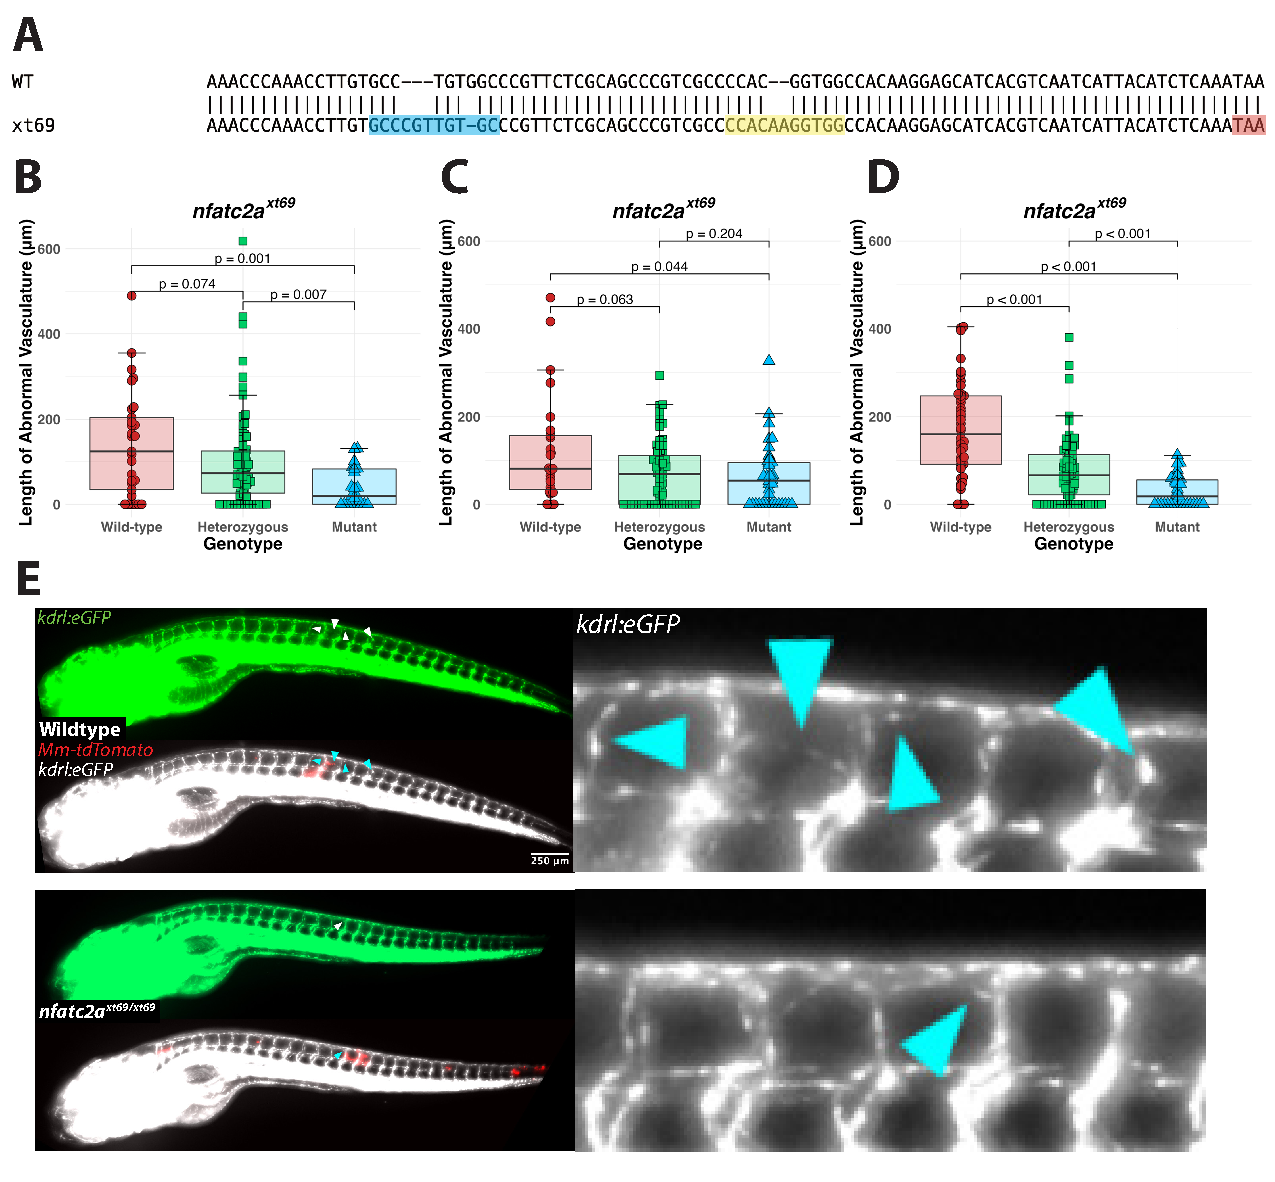
\includegraphics[width=\textwidth]{images/nfatc2alarvae.pdf}
\caption{\textit{nfatc2a} is required for the angiogenic response to infection. Use of the stable mutant line \textit{nfatc2a\textsuperscript{xt69}} demonstrated an important role for this pathway in inducing angiogenesis. (A) diagrams the mutation I established. (B), (C) and (D) show three replicates of the infection experiment, demonstrating robust and reproducible reduction in angiogenesis in both the heterozygous and mutant conditions relative to wild\hyp{}type. (E) shows a representative example of the effect seen, with robust angiogenesis under wild\hyp{}type conditions and a significant reduction with \textit{nfatc2a\textsuperscript{xt69/xt69}}.}
% Provide a label so we can cross\hyp{}reference it from the tex
\label{figure:c2larvae}
\end{figure}

We then established stable, germline transmitting indel mutant alleles for both genes to validate our results from mosaic animals. Recapitulating our results in the F\textsubscript{0} generation, the \textit{nfatc3a\textsuperscript{xt59}} mutation carrying a 22 bp deletion (leading to an early stop codon at amino acid 9 in exon 1) had no effect on angiogenesis at 4 days post infection (\autoref{figure:mosaic}D, E). We then developed a knockout line of \textit{nfatc2a} bearing a net 4 bp insertion leading to an early stop codon in the second exon (at amino acid 273, frameshifted after amino acid 247), prior to the DNA\hyp{}binding domain (\textit{nfatc2a\textsuperscript{xt69}}) (\autoref{figure:c2larvae}A). We repeated our angiogenesis assay using larvae from incrosses of \textit{kdrl}:\textit{eGFP}; \textit{nfatc2a\textsuperscript{xt69/+}} animals that produced expected Mendelian ratios of wild\hyp{}type, heterozygous, and homozygous mutant offspring. Consistent with the results from mosaic animals, homozygous knockout of \textit{nfatc2a} was sufficient to reduce the degree of angiogenesis present in larval zebrafish at 4 days post infection (\autoref{figure:c2larvae}B\hyp{}E). Importantly, given the known role of NFAT isoforms in T cell function, these defects emerged prior to the developmental emergence of functional T cells, which does not occur until approximately 6 days post fertilization as the thymus develops \citep{Trede2004}. However, whole animal knockouts could not address potential roles for cell types other than macrophages in mediating this process. 

\subsection{Macrophage\hyp{}NFAT is Essential for Angiogenesis Induction \textit{in vivo}}

\begin{figure}
\centering
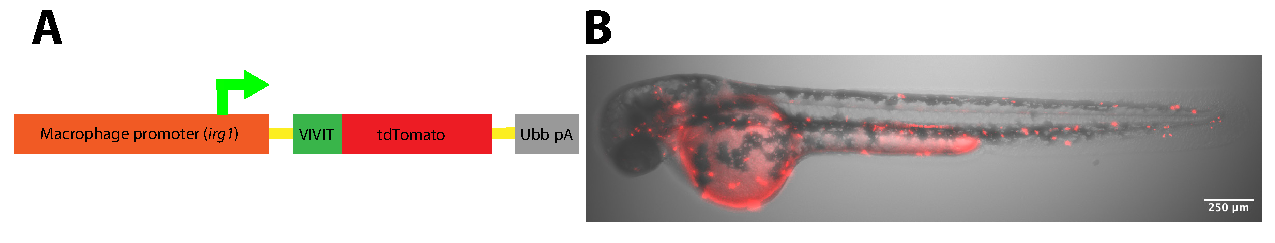
\includegraphics[width=\textwidth]{images/vivitconstruct.pdf}
\caption{Design of the \textit{irg1}:\textit{VIVIT\hyp{}tdTomato} construct. (A) shows the overall layout of the construct, with \textit{irg1} driving the expression of the VIVIT peptide conjugated to tdTomato. (B) shows a representative \textit{irg1}:\textit{VIVIT\hyp{}tdTomato\textsuperscript{xt38}} larva.}
% Provide a label so we can cross\hyp{}reference it from the tex
\label{figure:vivitdiagram}
\end{figure}

Given our observations on \textit{vegfaa} induction in macrophages at the granuloma, we tested whether NFAT signaling was required specifically in macrophages for granuloma\hyp{}associated angiogenesis. For \textit{in vivo} inhibition of macrophage NFAT signaling during infection, we applied an approach that takes advantage of the NFAT\hyp{}inhibitory peptide VIVIT which competitively inhibits calcineurin\hyp{}dependent activation of all the NFATc isoforms \citep{Aramburu1999}. This approach has been successfully used as an exogenous treatment in cell culture \citep{Deerhake2021} and mice \citep{Noguchi2004, Elloumi2012, Rojanathammanee2015}, through ectopic overexpression in cell culture \citep{McCullagh2004},  and, more recently, in mice \citep{Poli2022, Peuker2022}. We developed a transgenic zebrafish line in which VIVIT is expressed specifically in macrophages, Tg(\textit{irg1}:\textit{VIVIT\hyp{}tdTomato\textsuperscript{xt38}}) (from here, simply \textit{irg1}:\textit{VIVIT}) (\autoref{figure:vivitdiagram}A, B) \citep{Sanderson2015}. We assessed whether the macrophage\hyp{}specific expression of VIVIT would be sufficient to reduce the degree of angiogenesis during infection in the trunk with wild\hyp{}type \textit{M. marinum} expressing mCerulean (\textit{Mm}\hyp{}mCerulean). We found that macrophage\hyp{}specific VIVIT expression significantly reduced angiogenesis in response to infection (\autoref{figure:vivitinf}A\hyp{}D). This suggested a macrophage\hyp{}specific role for NFAT signaling downstream of mycobacterial detection that was necessary to induce angiogenesis, presumably through the \textit{nfatc2a} isoform.

\begin{figure}
\centering
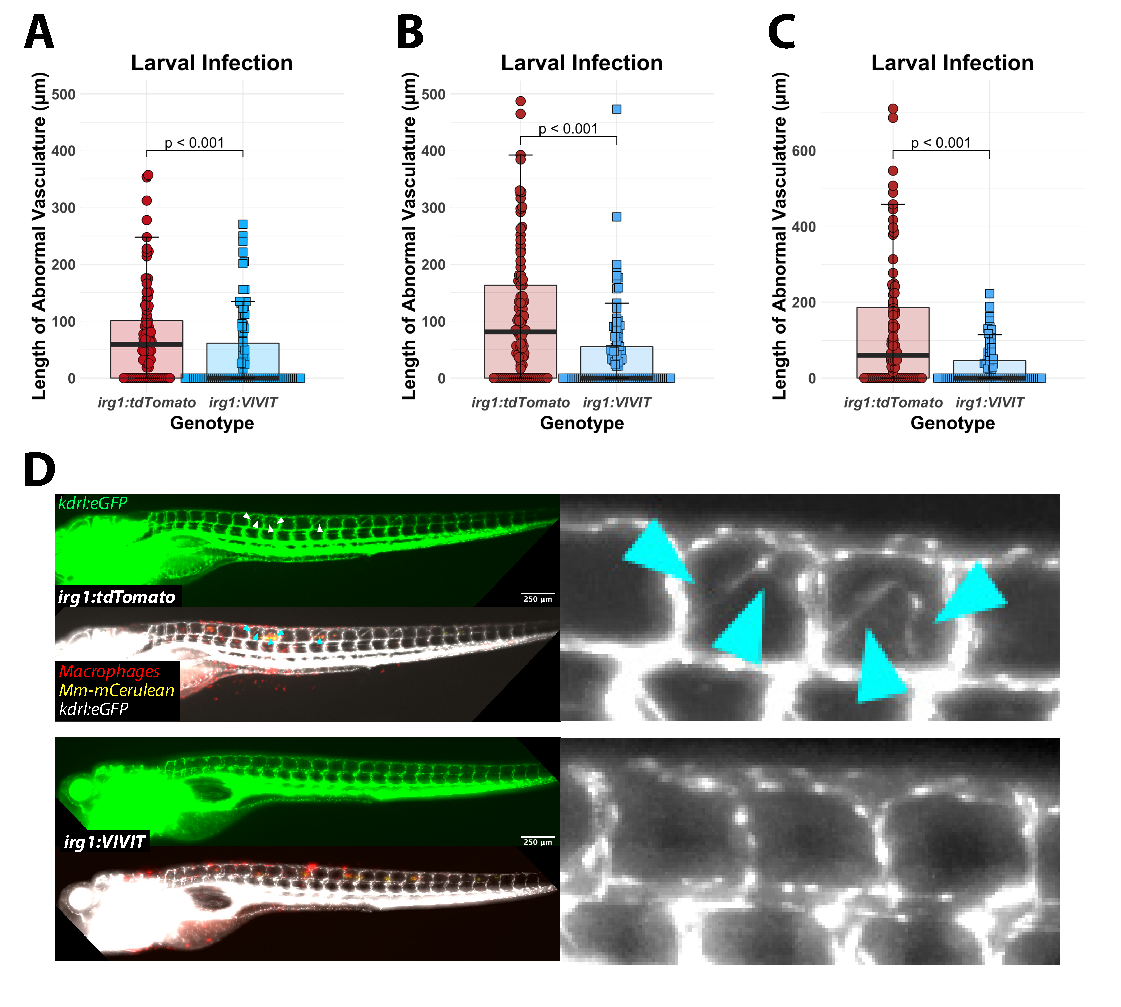
\includegraphics[width=\textwidth]{images/vivitlinf.pdf}
\caption{Macrophage\hyp{}specific VIVIT expression in larval zebrafish inhibits infection\hyp{}induced angiogenesis. (A), (B), and (C) show three replicates of this infection experiment and a robust reduction in the amount of angiogenesis with expression of the VIVIT peptide compared to \textit{irg1}:\textit{tdTomato}\hyp{}only controls. (D) shows representative images o the effect observed, with reduced angiogenesis seen in the VIVIT condition.}
% Provide a label so we can cross\hyp{}reference it from the tex
\label{figure:vivitinf}
\end{figure}

To ask more directly whether the decreased angiogenesis observed in the NFAT\hyp{}deficient macrophages was via the TDM\hyp{}mediated pathway, we used the TDM injection assay we had developed previously. We injected TDM or the IFA vehicle into the trunk of 2 days post fertilization larval zebrafishand measured the resulting angiogenesis at 2 days post injection \citep{Walton2018}. TDM was sufficient to induce angiogenesis \textit{in vivo} and this effect was dependent upon functional NFAT signaling, with the degree of TDM\hyp{}induced angiogenesis reduced to the level of the vehicle alone in \textit{irg1}:\textit{VIVIT\hyp{}tdTomato} animals compared to \textit{irg1}:\textit{tdTomato} controls (\autoref{figure:vivittdm}A\hyp{}D).

\begin{figure}
\centering
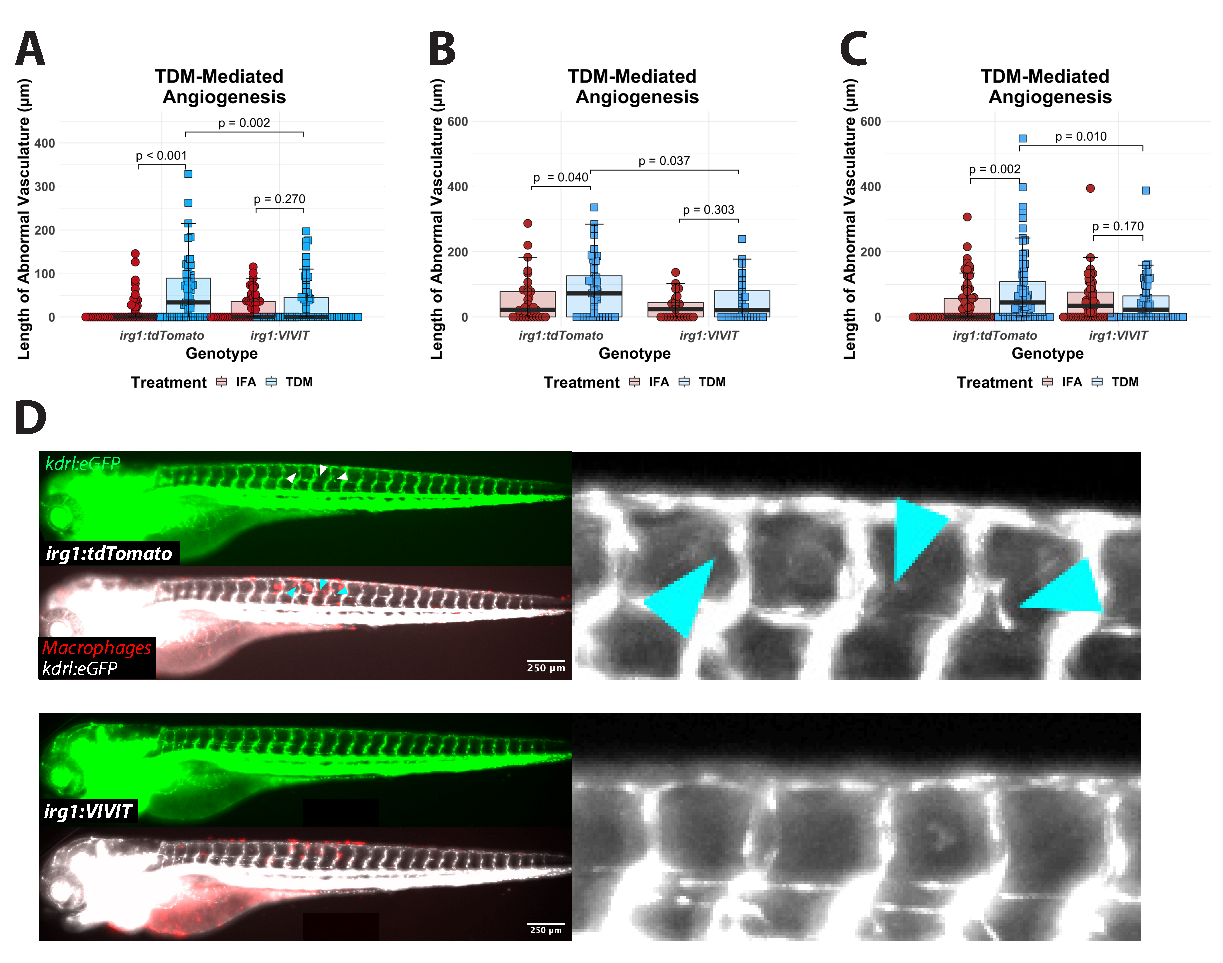
\includegraphics[width=\textwidth]{images/vivittdm.pdf}
\caption{Macrophage\hyp{}specific VIVIT expression reduces TDM\hyp{}induced angiogenesis in the larval zebrafish. (A), (B), and (C) display three independent replicates of this experiment; (D) demonstrates the effect by representative images showing the reduction seen in the VIVIT\hyp{}expressing condition.}
% Provide a label so we can cross\hyp{}reference it from the tex
\label{figure:vivittdm}
\end{figure}

\subsection{NFAT Activation is Essential for Angiogenesis in Adult Granulomas}\label{nfatc2aAdult}

\begin{figure}
\centering
\includegraphics[width=\textwidth]{images/adultinf.pdf}
\caption{Schematic of the infection and CLARITY\hyp{}clearing approach used for adult infection experiments. Adult zebrafish (>12 weeks post fertilization) are infected interperitoneally with ~500 CFU of fluorescent \textit{M. marinum} and then organs are harvested and fixed approximately 14 days later, cleared with detergent, and then imaged.}
% Provide a label so we can cross\hyp{}reference it from the tex
\label{figure:adult}
\end{figure}

Adult zebrafish are equipped with both innate and adaptive immunity and form mycobacterial granulomas that histologically mirror epithelioid human tuberculosis granulomas \citep{Swaim2006}, including induction of a surrounding vascular network \citep{Cronan2015}. To assess whether our findings in the larvae translated to a longer\hyp{}term context in the presence of adaptive immunity, we infected adult \textit{kdrl}:\textit{eGFP}; \textit{nfatc2a\textsuperscript{xt69/xt69}} zebrafish and \textit{kdrl}:\textit{eGFP}; \textit{nfatc2a\textsuperscript{+/+}} siblings with \textit{Mm}\hyp{}tdTomato and examined their peritoneal organs at 18 days post infection after CLARITY\hyp{}based clearing \citep{Chung2013, Cronan2015}. Cleared organs were then imaged by spinning disk confocal microscopy (\autoref{figure:adult}). We measured the total vascular network surrounding the granulomas in a programmatically blinded fashion (\citet{Salter2016} and \autoref{blinders}) and found that \textit{nfatc2a\textsuperscript{xt69/xt69}} fish had a significant reduction (${\sim}$50\%) in the length of the vascular network compared to wild\hyp{}type siblings, further validating this gene as important for the angiogenic response \textit{in vivo} (\autoref{figure:c2adult}A\hyp{}D). These putatively neovascular vessels tend to be highly branched and to be comprised of a limited number of cells with small or non\hyp{}existent luminal volume, indicating that they are still in the sprouting stage of angiogenesis and suggesting a potential failure to mature over time, perhaps indicative of leakiness or other vascular defects, although further characterization would be required. We observed robust effects that are likely understated in our quantitation, as we could not make any formal distinction between thicker, existing vasculature present at baseline that happens to fall nearby the granuloma and the characteristic neovascularization more intimately associated with the granuloma and present in wild\hyp{}type but reduced in \textit{nfatc2a} mutants (\autoref{figure:grandiv}).

\begin{figure}
\centering
\includegraphics[width=\textwidth]{images/nfatc2aadult.pdf}
\caption{\textit{nfatc2a} is required for robust angiogenesis in established granulomas. (A) shows images comparing wild\hyp{}type and \textit{nfatc2a\textsuperscript{xt69/xt69}} granulomas and a substantial reduction in the overall angiogenic effect can be seen. This is quantitated in (B), (C), and (D), with an ~50\% reduction in the total vasculature visible in the proximity of each granuloma.}
% Provide a label so we can cross\hyp{}reference it from the tex
\label{figure:c2adult}
\end{figure}

\begin{figure}
\centering
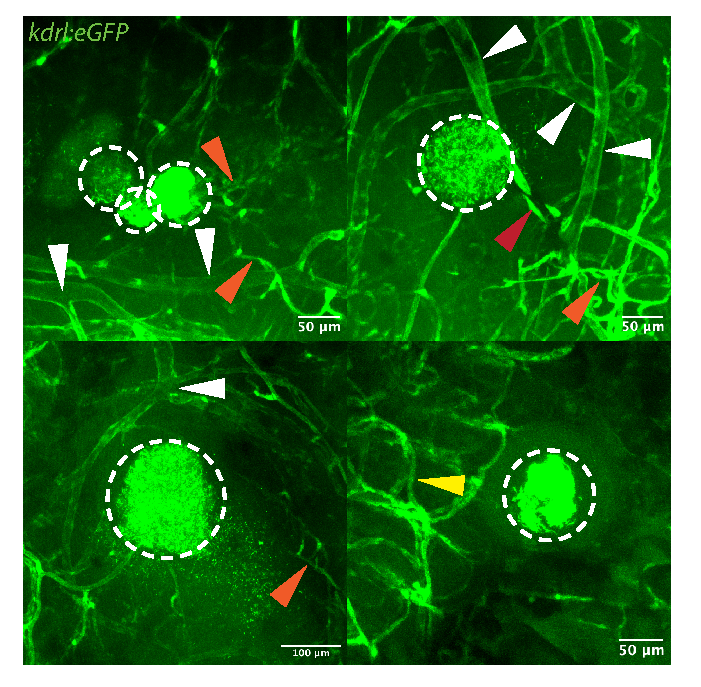
\includegraphics[width=\textwidth]{images/grandiv.pdf}
\caption{Mycobacterial granulomas display significant heterogeneity in vascularization and many are in physical proximity to mature, likely pre\hyp{}existing vessels. One of the drawbacks of the adult angiogenesis measurements is significant background seen in the proximity of these granulomas, as seen in this figure.}
% Provide a label so we can cross\hyp{}reference it from the tex
\label{figure:grandiv}
\end{figure}

\subsection{\mbox{Macrophage\hyp{}specific} NFAT Inhibition in Mature Granulomas Reduces Angiogenesis}

We next evaluated whether macrophage\hyp{}specific NFAT inhibition had similar effects on vascularization in adult zebrafish. We infected adult \textit{irg1}:\textit{tdTomato}; \textit{kdrl}:\textit{eGFP} and \textit{irg1}:\textit{VIVIT\hyp{}tdTomato}; \textit{kdrl}:\textit{eGFP} double transgenic zebrafish with \textit{Mm}\hyp{}mCerulean and examined visceral organs at 14 days post infection. We used confocal imaging to visualize individual CLARITY\hyp{}cleared organs and measured the total length of granuloma\hyp{}proximal vasculature under blinding as above (Salter, 2016). We found that the degree of vascularization was significantly reduced around granulomas from \textit{irg1}:\textit{VIVIT\hyp{}tdTomato} fish as compared to \textit{irg1}:\textit{tdTomato} fish (\autoref{figure:vivitadult}A\hyp{}D). The extent of the vascular network in the \textit{irg1}:\textit{VIVIT\hyp{}tdTomato} condition was notably restricted in most cases or solely comprised of more mature, luminal vessels, suggesting a total failure to induce an angiogenic response (\autoref{figure:vivitadult}A). These findings, consistent with our previous data from both larval zebrafish infections in the \textit{irg1}:\textit{VIVIT\hyp{}tdTomato} background and in the \textit{nfatc2a} mutant adult fish, point to a critical role for macrophage\hyp{}specific NFAT activation in inducing the angiogenic response at mycobacterial granulomas. Furthermore, this establishes that NFAT function is broadly conserved from early larval infection through to the mature necrotic granulomas that characterize adult infection.

\begin{figure}
\centering
\includegraphics[width=\textwidth]{images/vivitadult.pdf}
\caption{Macrophage\hyp{}VIVIT expression inhibits granuloma angiogenesis in the adult zebrafish infection model. (A) shows images comparing \textit{irg1}:\textit{tdTomato} and \textit{irg1}:\textit{VIVIT\hyp{}tdTomato} granulomas and a substantial reduction in the overall angiogenic effect can be seen. This is quantitated in (B), (C), and (D), with an ~50\% reduction in the total vasculature visible in the proximity of each granuloma.}
% Provide a label so we can cross\hyp{}reference it from the tex
\label{figure:vivitadult}
\end{figure}

\subsection{Inhibition of NFAT Signaling Results in Decreased Bacterial Burden}

We had previously shown that inhibition of granuloma\hyp{}associated vascularization is associated with decreased bacterial burden. Mycobacterial mutants unable to induce vascularization ($\upDelta$\textit{pcaA}), and either genetic or pharmacological inhibition of VEGF or CXCR4 signaling all result in lower bacterial burden, presumably due to functions of the aberrant vasculature promoting bacterial growth and/or inhibiting bacterial killing \citep{Rao2005, Glickman2000, Oehlers2015, Walton2018} or through more direct pro\hyp{}bacterial activities of VEGFA \citep{Harding2019}. To examine the effect on burden of inhibition of NFAT signaling, we performed colony forming unit (CFU) assays at timepoints after the induction of angiogenesis and granuloma maturation. We infected \textit{nfatc2a\textsuperscript{+/+}} and \textit{nfatc2a\textsuperscript{xt69/xt69}} adult zebrafish with \textit{Mm}\hyp{}tdTomato and plated them for CFU at 24 days post infection. We found that knockout of \textit{nfatc2a} resulted in a ${\sim}$50\% decrease in median colony number compared to wild\hyp{}type after extended infection (\autoref{figure:cfu}A). 

\begin{figure}
\centering
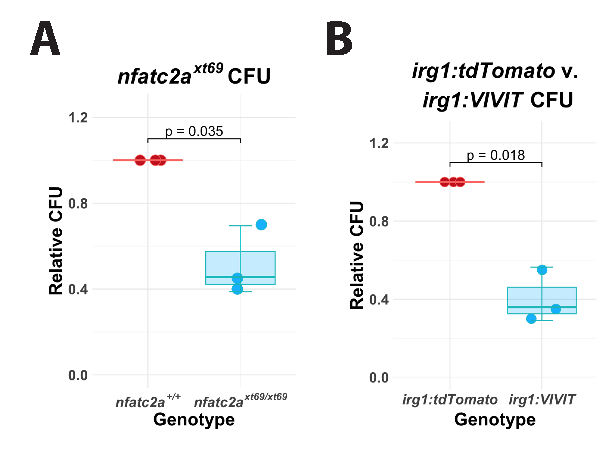
\includegraphics[height=3in]{images/cfu.pdf}
\caption{Inhibition of NFAT signaling results in a reduction in mycobacterial CFU at time points after granuloma formation. (A) shows a reduction in bacterial burden in \textit{nfatc2a} mutant fish while (B) shows a similar reduction in burden in VIVIT\hyp{}expressing fish.}
% Provide a label so we can cross\hyp{}reference it from the tex
\label{figure:cfu}

\end{figure}

Finally, we evaluated the impact of macrophage\hyp{}specific NFAT inhibition on whole organism bacterial burden. We infected adult zebrafish possessing either the \textit{irg1}:\textit{tdTomato} or \textit{irg1}:\textit{tdTomato} transgenes with \textit{Mm}\hyp{}tdTomato and then homogenized and plated these fish at 18 days post infection. We found that macrophage expression of the VIVIT peptide resulted in a median reduction of ${\sim}$60\% of the bacterial burden in these fish at this time point relatively soon after the formation of necrotic granulomas and robust induction of angiogenesis (\autoref{figure:cfu}B).
 
\subsection{Pharmacological Inhibition of NFAT in Human \mbox{THP\hyp{}1} Macrophages Limits VEGFA Induction by \textit{Mycobacterium tuberculosis}}\label{thp1inca}

\begin{figure}
\centering
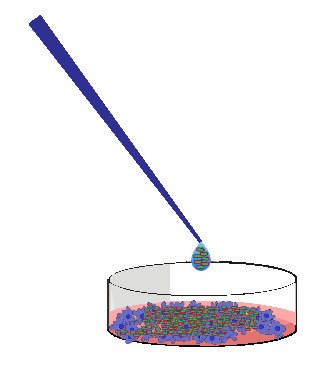
\includegraphics[height=2in]{images/gammamtbthp1model.pdf}
\caption{In our extracellular exposure model, clumps of gamma\hyp{}irradiated \textit{M. tuberculosis} is added to monolayers of THP\hyp{}1 macrophages to stimulate them via primarily extracellular exposure rather than by phagocytosis.}
% Provide a label so we can cross\hyp{}reference it from the tex
\label{figure:exposure}
\end{figure}

The zebrafish mycobacterial infection model shares important conserved features with \textit{M. tuberculosis} infection of humans, host response and granuloma angiogenesis \citep{Swaim2006, Datta2015, Oehlers2015, Cronan2021}. In addition, important aspects of the response to cyclopropanated TDM appears to be largely maintained between zebrafish and humans \citep{Walton2018, Rao2005}. We next asked whether our findings discovered \textit{in vivo} with the zebrafish\hyp{}\textit{M. marinum} model were conserved in human cells exposed to \textit{M. tuberculosis}. We developed a cell culture model of macrophage\hyp{}\textit{M. tuberculosis} interactions using differentiated THP\hyp{}1 monocytic cells exposed to $\upgamma$\hyp{}irradiated \textit{Mycobacterium tuberculosis} H37Rv ($\upgamma$\textit{Mtb}), which produces the full spectrum of TDM species, presented to the cell in their native configuration (as compared to heat\hyp{}killed \textit{M. tuberculosis}, which disrupts cell envelope structure and organization) \citep{Romero2014, SecanellaFandos2014} (\autoref{figure:exposure}) (\autoref{tdm}). We found that exposure of differentiated THP\hyp{}1 macrophages to $\upgamma$\textit{Mtb} was sufficient to induce VEGFA transcription as well as VEGFA secretion (\autoref{figure:qpcr}A\hyp{}C, \autoref{figure:elisa}A\hyp{}C). To examine whether NFAT signaling is required for production and secretion of VEGFA we treated THP\hyp{}1 macrophages with the small molecule inhibitor INCA\hyp{}6, which specifically disrupts the interaction between the NFAT family members and their activating phosphatase, calcineurin \citep{Roehrl2004a, Roehrl2004b}. Strikingly, treatment of THP1 cells with INCA\hyp{}6 during $\upgamma$\textit{Mtb} exposure significantly inhibited transcriptional induction of \textit{VEGFA} (\autoref{figure:qpcr}A\hyp{}C), as well as VEGFA secretion (\autoref{figure:elisa}A\hyp{}C). Immunofluorescence revealed robust translocation of NFAT (using an NFATC2 antibody) that was broadly correlated to VEGFA signal (\autoref{figure:incaif}A\hyp{}D, \autoref{figure:incaquant}A\hyp{}C). Taken together these experiments suggest that human NFAT signaling is required for VEGF production in response to \textit{M. tuberculosis} exposure.

\begin{figure}
\centering
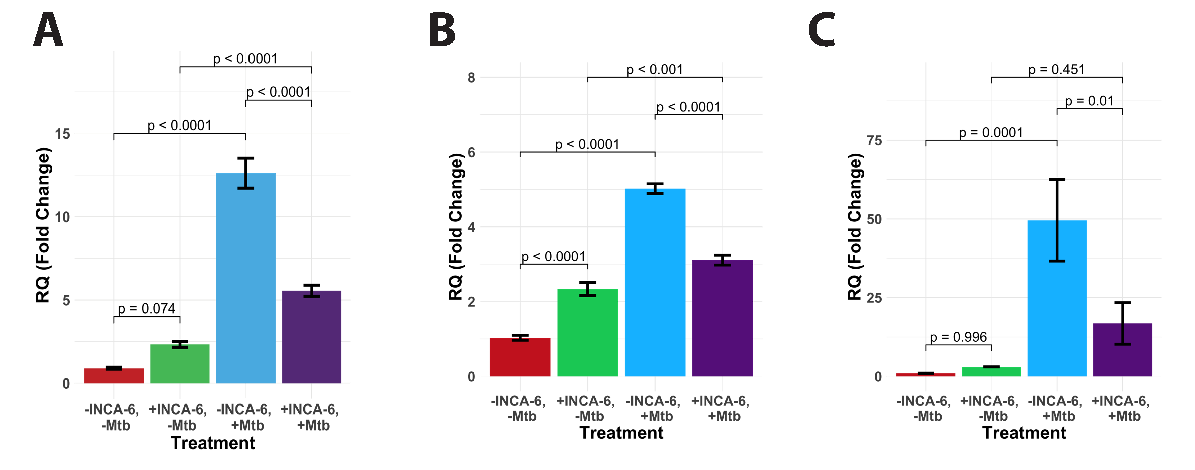
\includegraphics[width=\textwidth]{images/incaqpcr.pdf}
\caption{Treatment of THP\hyp{}1 macrophages with gamma\hyp{}irradiated \textit{M. tuberculosis} results in the induction of \textit{VEGFA} that is sensitive to inhibition by INCA\hyp{}6, a calcineurin\hyp{}NFAT inhibitor. Three independent replicates are shown in (A), (B), and (C).}
% Provide a label so we can cross\hyp{}reference it from the tex
\label{figure:qpcr}

\end{figure}

\begin{figure}
\centering
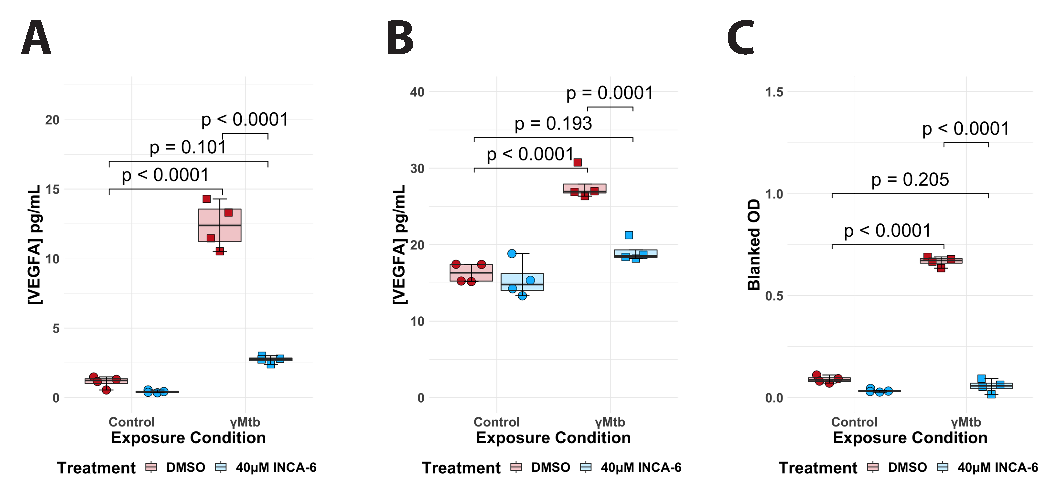
\includegraphics[width=\textwidth]{images/incaelisa.pdf}
\caption{Treatment of THP\hyp{}1 macrophages with gamma\hyp{}irradiated \textit{M. tuberculosis} results in the secretion of VEGFA and is sensitive to inhibition by INCA\hyp{}6, a calcineurin\hyp{}NFAT inhibitor. Three independent replicates are shown in (A), (B), and (C). The standard curve for the replicate in C was generated improperly and was unable to be used, so raw blanked OD values are provided instead.}
% Provide a label so we can cross\hyp{}reference it from the tex
\label{figure:elisa}

\end{figure}

\begin{figure}
\centering
\includegraphics[height=5in]{images/incaIF.pdf}
\caption{Immunofluorescence imaging of gamma\hyp{}irradiated \textit{M. tuberculosis} exposed THP\hyp{}1 macrophages reveals robust NFAT protein translocation into the nucleus after exposure that corresponds to the induction of VEGFA. (A) shows robust VEGFA induction that can be inhibited by addition of INCA\hyp{}6. (B) shows a magnified view of the NFAT nuclear translocation seen in (A). (C) shows further images and the correspondence between NFAT activation and VEGF production. (D) shows the reduction in nuclear localization from the images seen in (C).}
% Provide a label so we can cross\hyp{}reference it from the tex
\label{figure:incaif}

\end{figure}

\begin{figure}
\centering
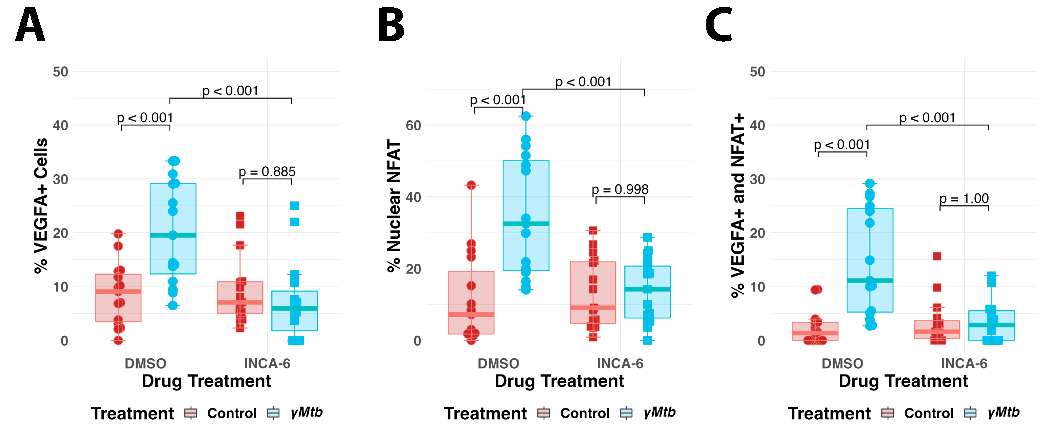
\includegraphics[width=\textwidth]{images/incaIFquant.pdf}
\caption{Quantitation of various aspects of the response seen by immunofluorescence after gamma\hyp{}irradiated \textit{M. tuberculosis}\hyp{}exposure and INCA\hyp{}6 treatment. (A) shows the overall percentage of VEGFA+ cells seen in each condition, with a significant increase with $\upgamma$\textit{Mtb} exposure that is inhibited by INCA\hyp{}6. (B) shows a parallel phenotype, where $\upgamma$\textit{Mtb} induces NFAT nuclear localization that is sensitive to INCA\hyp{}6 addition. (C) shows the percentage of the total cells in the field of view that demonstrate both NFAT nuclear localization and VEGF expression.}
% Provide a label so we can cross\hyp{}reference it from the tex
\label{figure:incaquant}
\end{figure}

\subsection{Requirement of human NFATC2 for VEGFA induction}\label{thp1lenti}

To identify functionally important NFAT human isoforms, we exposed THP\hyp{}1 macrophages to $\upgamma$\textit{Mtb} and subsequently used the secretion inhibitor brefeldin A to lock VEGFA within secreting cells. Simultaneous staining for each of the four human NFATc proteins along with VEGFA allowed us to identify NFAT isoforms that underwent changes in expression and localization and correlate this with VEGFA production (\autoref{figure:isoforms}A). While THP\hyp{}1 macrophages express all of the isoforms to varying degrees, the most intense co\hyp{}staining with VEGF was found with NFATC2 (\autoref{figure:isoforms}B). Additionally, while each of the isoforms displayed structural and localization alterations (albeit not always nuclear) after $\upgamma$\textit{Mtb} exposure, only NFATC2 showed robust nuclear localization that appeared to correspond to VEGFA induction in individual cells (\autoref{table:isoforms}). While some NFAT isoform translocation was observable with at least NFATC1 and, minorly, NFATC3, this generally had, at best, modest correspondence to the degree or presence of VEGFA production (\autoref{figure:isoformsquant}). While NFATC1 was correlated with VEGFA induction, the effect was much weaker than that seen with NFATC2. We quantified this effect by counting the number of VEGFA\hyp{}expressing, NFAT nuclear localized cells and normalized to the number of VEGFA\hyp{}expressing cells in total and found that NFATC2 most tightly corresponded to the induction of VEGFA in $\upgamma$\textit{Mtb}\hyp{}exposed cells \autoref{figure:isoformsquant}. Given the strong correlation for NFATC2 with nuclear localization and VEGFA production after $\upgamma$\textit{Mtb} exposure, expression data from zebrafish and non\hyp{}human primate granulomas, as well as the \textit{in vivo} zebrafish results implicating macrophage \textit{nfatc2a} in \textit{vegfaa} production and angiogenesis, we focused on human NFATC2 as the key isoform.

\singlespacing

\begin{center}
\begin{table}[h]
\caption{Relative correspondence between the nuclear localization and VEGFA induction across all four NFAT isoforms. We observed nice correspondence between NFATC2 and VEGFA and a lesser association between NFATC1 and VEGFA while the other two isoforms displayed no notable relationship between their nuclear localization and VEGFA induction.}
\label{table:isoforms} \tabularnewline
\vspace{0.5cm}
\begin{tabular}{|p{1in}|p{0.75in}|p{0.75in}|p{3in}|}
\hline
 & \thead{\hyp{}$\upgamma$\textit{Mtb}} & \thead{+$\upgamma$\textit{Mtb}} & \thead{Relationship to VEGFA?} \tabularnewline
\hline
NFATC1 & + & ++ & Modest relationship between nuclear localization and VEGF expression. \tabularnewline
\hline
NFATC2 & ++ & +++ & Nuclear localization generally corresponds to VEGF expression. \tabularnewline
\hline
NFATC3 & + & ++ & Weak relationship between nuclear localization and VEGF expression. \tabularnewline
\hline
NFATC4 & +/\hyp{} & + & Expression increased but not obviously nuclear in most cells. \tabularnewline
\hline
\end{tabular}
\end{table}
\end{center}

\doublespacing

\begin{figure}
\centering
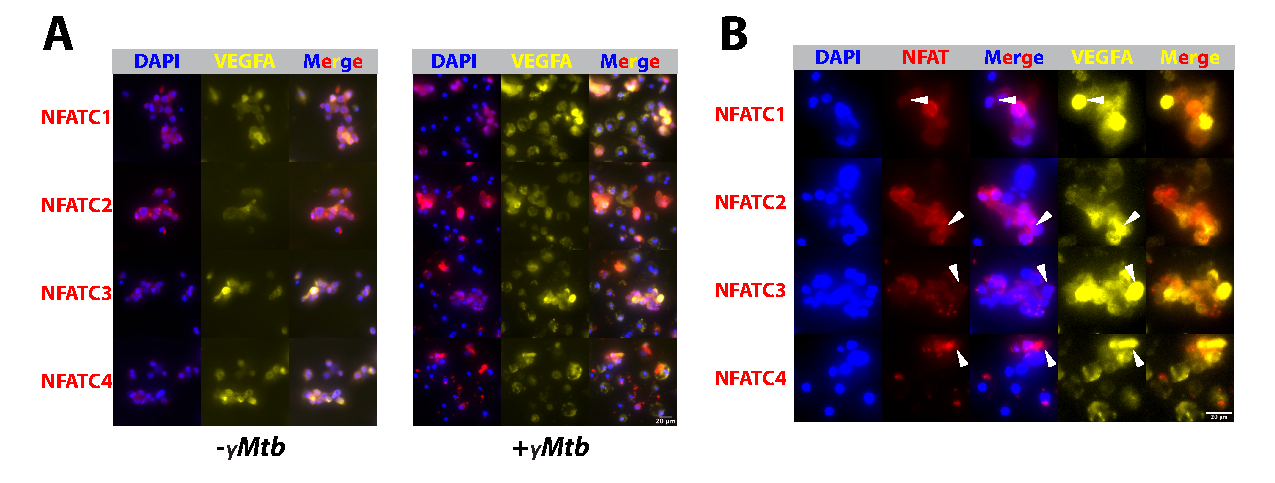
\includegraphics[width=\textwidth]{images/isoformsIF.pdf}
\caption{To identify particular NFAT isoforms that may be important for VEGFA production downstream of \textit{M. tuberculosis} detection, immunofluorescence was performed against each of the isoforms. NFATC2 showed the most consistent induction of all of the isoforms. (A) shows alterations in the protein production and localization with and without \textit{M. tuberculosis}. (B) displays a representative field where multiple VEGFA\hyp{}expressing cells can be seen, but only nuclear localization of NFATC2 seems to correspond with this expression.}
% Provide a label so we can cross\hyp{}reference it from the tex
\label{figure:isoforms}
\end{figure}

\singlespacing

\begin{center}
\begin{table}[h]
\caption{Nearest gene neighbors for the ST sgRNAs (all are intergenic).}
\label{table:targets} \tabularnewline
\vspace{0.5cm}
\begin{tabular}{|p{1in}|p{4in}|}
\hline
\thead{sgRNA} & \thead{Nearest Gene Neighbor (Chromosome)} \tabularnewline
\hline
hU6 ST & CNTN1 (12) \tabularnewline
\hline
mU6 ST & MTDH (8) \tabularnewline
\hline
7SK ST & OPN5 (6) \tabularnewline
\hline
hH1 ST & ENSG00000249941 (5) \tabularnewline
\hline
\end{tabular}
\end{table}
\end{center}

\doublespacing

\begin{figure}
\centering
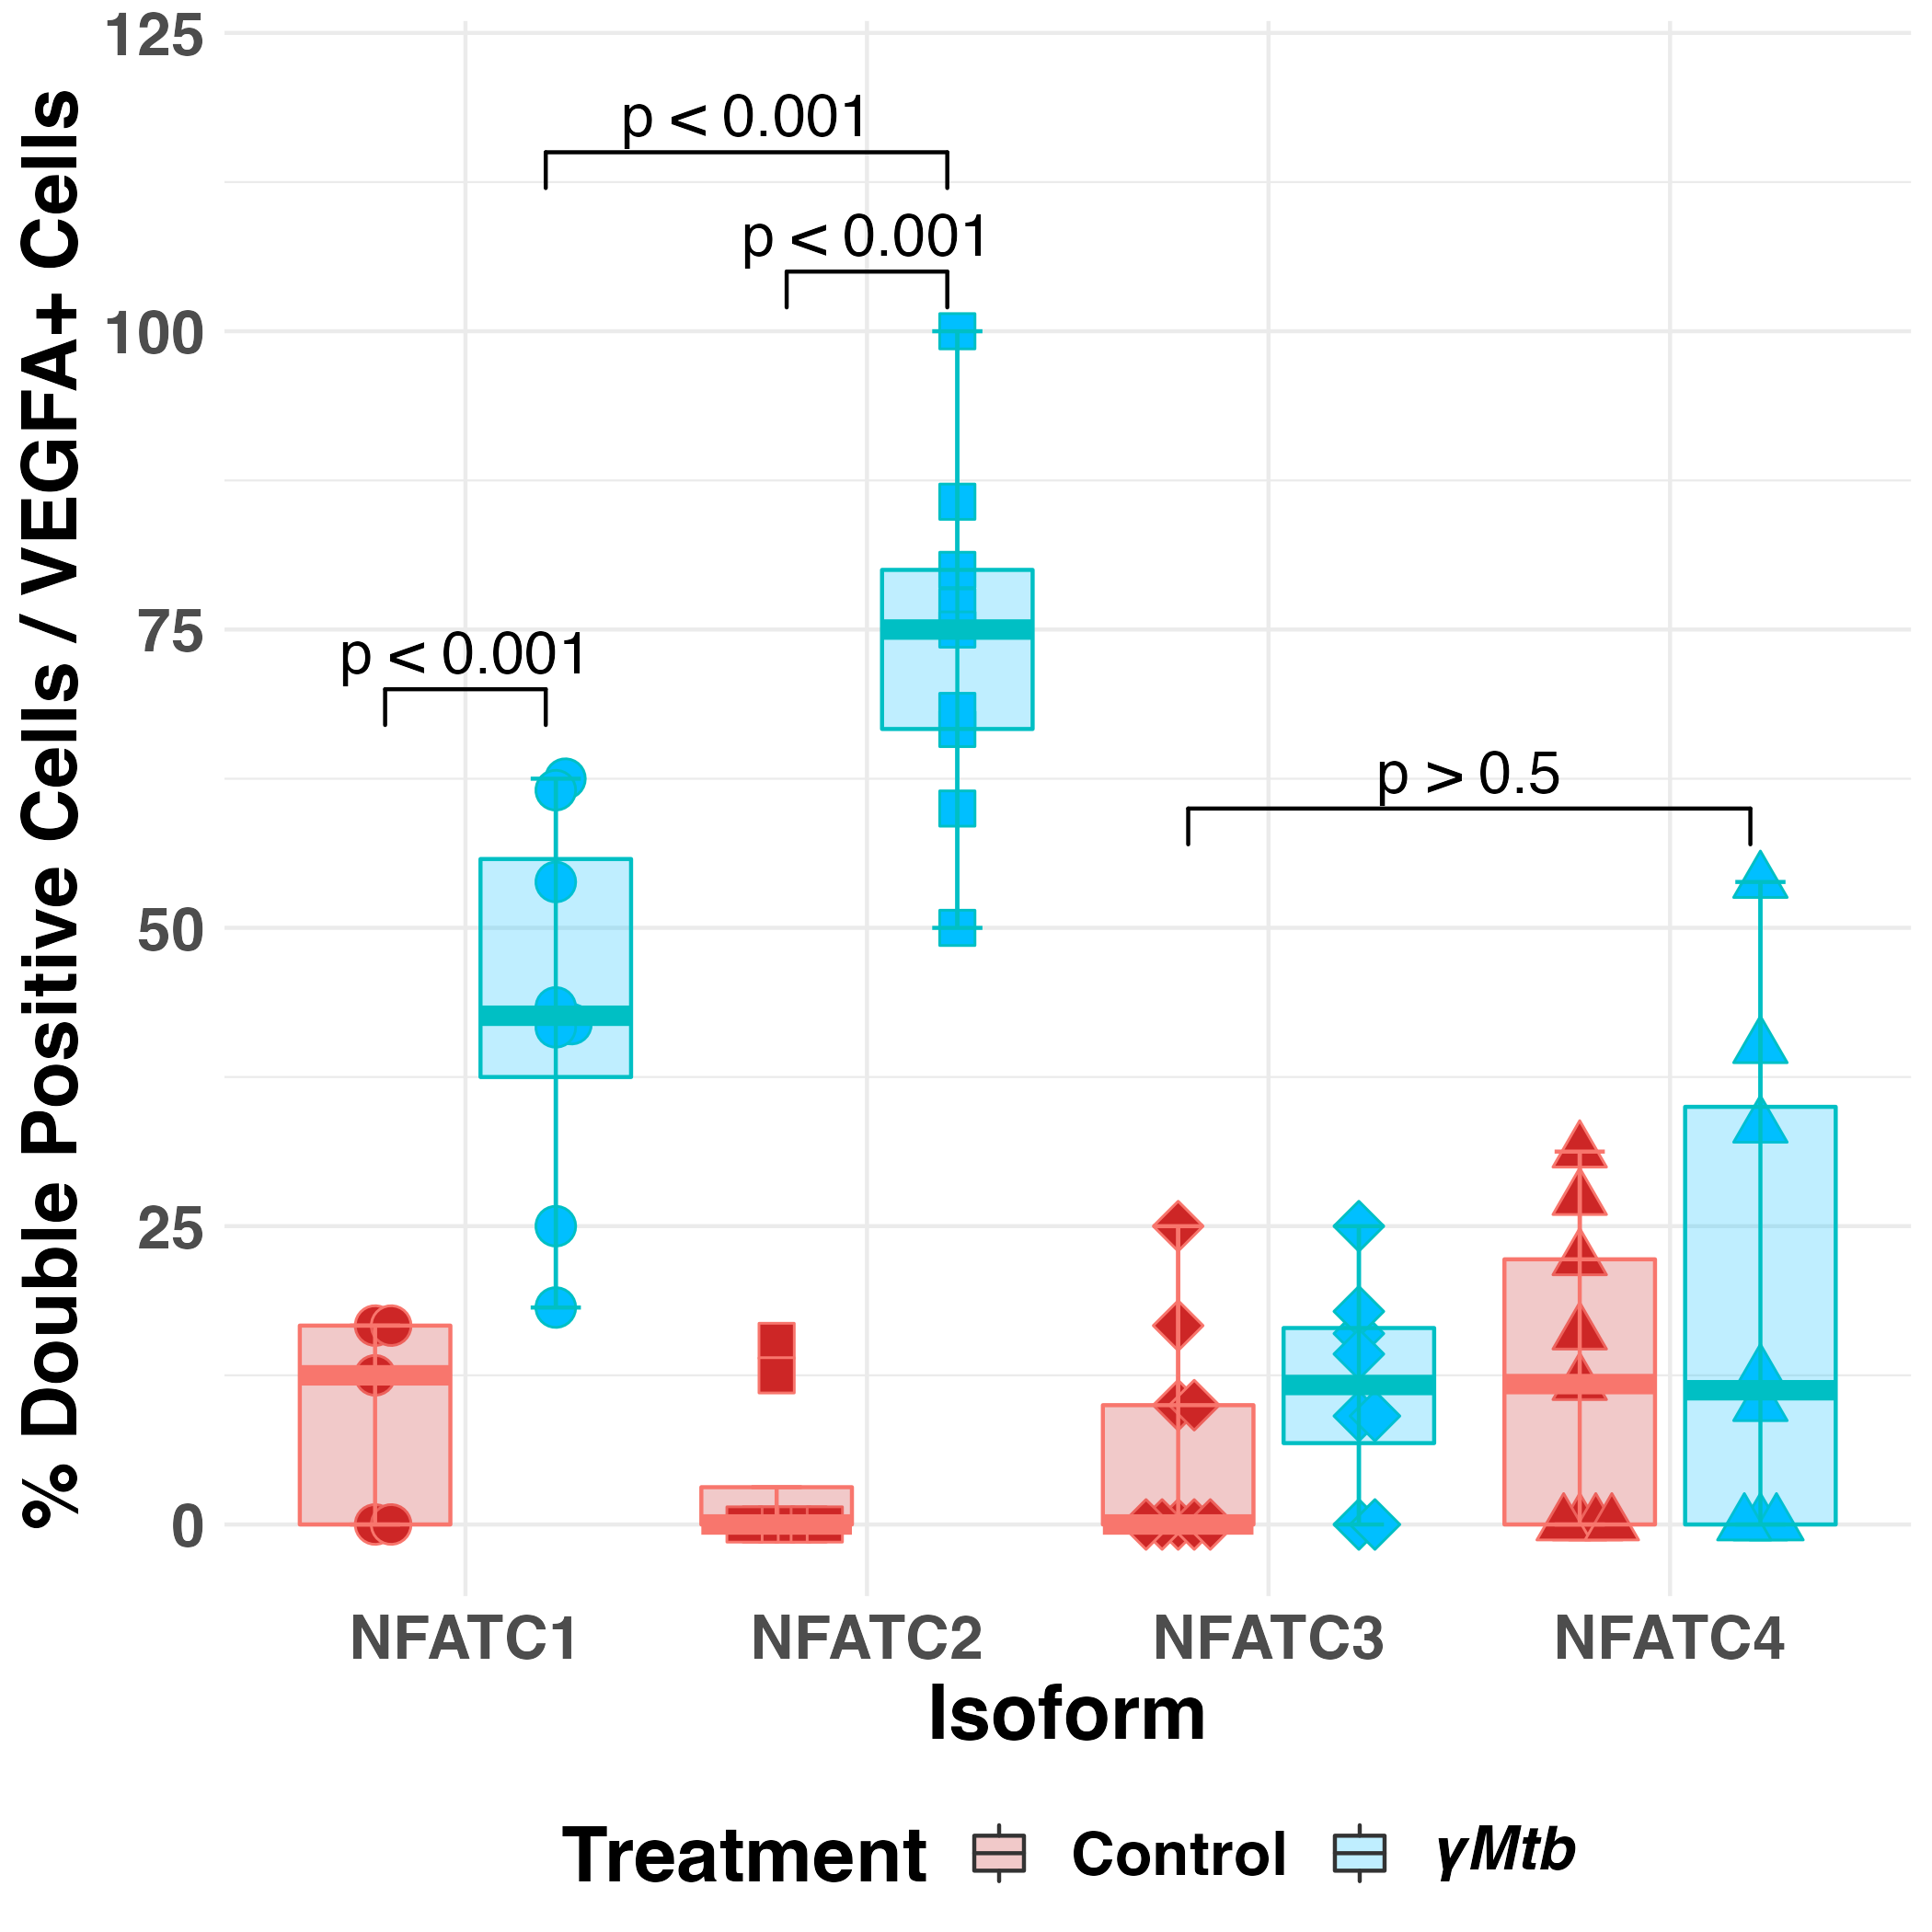
\includegraphics[height=3in]{images/NFAT_isoforms_110222.png}
\caption{We quantitated the immunofluorescence images from THP\hyp{}1 macrophages stained with antibodies against the four NFAT isoforms to assess the contribution of each protein to the VEGFA expression phenotype. Indeed, we found that NFATC2 most tightly corresponded to VEGFA induction by measuring double positive cells (those with both VEGFA expression and NFAT nuclear localization) and normalized to the total number of VEGFA positive cells.}
% Provide a label so we can cross\hyp{}reference it from the tex
\label{figure:isoformsquant}
\end{figure}

To test a functional role for human NFATC2 in macrophage induction of VEGFA during $\upgamma$\textit{Mtb} exposure, we used a lentivirus\hyp{}mediated CRISPR/Cas9 approach to introduce high\hyp{}efficiency disruption of NFATC2. Using techniques inspired by the zebrafish and backported to cell culture, we simultaneously expressed four distinct guide RNAs targeting NFATC2 or safe\hyp{}targeting controls, to maximize the percentage of puromycin\hyp{}resistant cells possessing complete null mutations \citep{Wu2018}. We compared these cells to those transduced with lentiviruses expressing safe\hyp{}targeting control sgRNAs. (\autoref{figure:targets}, \autoref{table:targets}, \autoref{lenti}) \citep{Kabadi2014, Sanjana2014, Morgens2017, Kitamura2021}. Due to technical challenges associated with long\hyp{}term culture of THP\hyp{}1 cells and to address heterogeneity among cellular responses, we focused these assays on VEGFA induction in these cells by immunofluorescence after $\upgamma$\textit{Mtb} exposure. Because the N\hyp{}terminal epitope recognized by our NFATC2 antibody was upstream of the targeted sites, we were unable to examine functional protein levels directly and simultaneously in the immunofluorescence images (\autoref{figure:validation}A). However, we found that transduced cells targeted by NFATC2 lentivirus generally failed to induce VEGFA while safe\hyp{}targeting control lentivirus\hyp{}transduced cells responded normally (\autoref{figure:lenti}A\hyp{}B), an effect that can be quantitated by percentage of VEGFA+ cells by multiple metrics (\autoref{figure:lentiIFquant}A\hyp{}C). These cells also demonstrated evidence of nonsense\hyp{}mediated decay by NFATC2 transcript levels (\autoref{figure:validation}B). Thus, macrophage NFATC2\hyp{}mediated induction of VEGFA downstream of mycobacterial TDM exposure is conserved from zebrafish to human cells exposed to \textit{M. tuberculosis}.

\begin{figure}
\centering
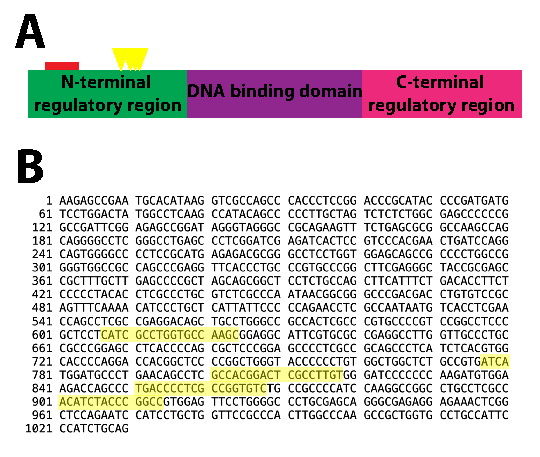
\includegraphics[height=2in]{images/lentitargets.pdf}
\caption{Based on our findings in THP\hyp{}1 macrophages and the larval zebrafish, NFATC2 was selected for genetic targeting in the THP\hyp{}1 macrophages. (A) displays the location of the four sgRNAs selected (in yellow arrows) and the location of the antibody epitope (red bar). (B) shows, on the genomic sequence itself, the location of the four sgRNAs.}
% Provide a label so we can cross\hyp{}reference it from the tex
\label{figure:targets}
\end{figure}

\begin{figure}
\centering
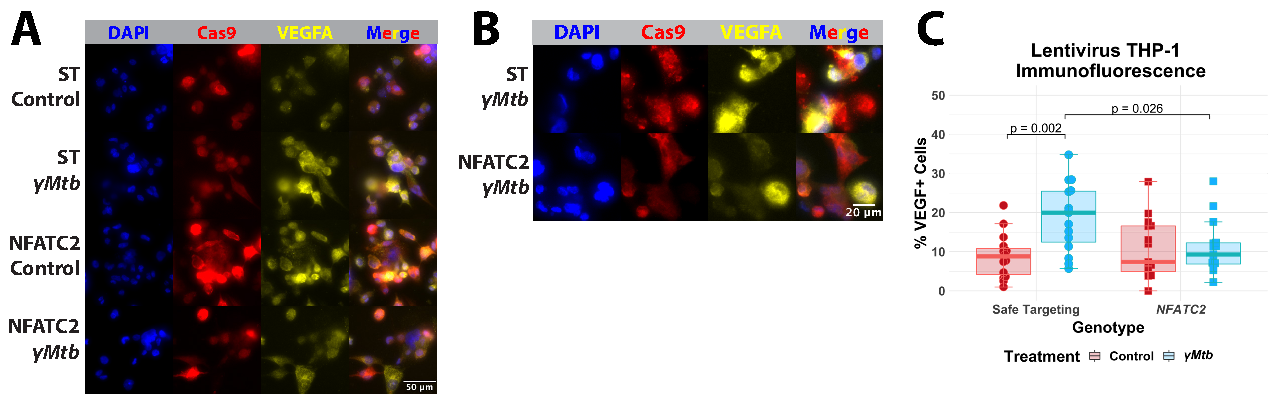
\includegraphics[width=\textwidth]{images/lentiIF.pdf}
\caption{Lentivirus\hyp{}mediated CRISPR/Cas9 targeting of NFATC2 results in reduced VEGFA expression after gamma\hyp{}irradiated \textit{M. tuberculosis} exposure. (A) shows that Cas9\hyp{}expressing NFATC2\hyp{}targeted cells have a reduction in VEGFA production while similar Cas9\hyp{}expressing cells with safe targeting control sgRNAs robustly induce VEGFA. (B) shows this magnified. Note the higher\hyp{}expressing NFATC2\hyp{}targeted cell has minimal Cas9 expression, suggesting that these effects may depend on the efficiency of targeting and other factors. (C) shows quantitation of the percentage of VEGFA+ cells in a given field of view, with a statistically significant reduction in the NFATC2\hyp{}targeted condition.}
% Provide a label so we can cross\hyp{}reference it from the tex
\label{figure:lenti}
\end{figure}

\begin{figure}
\centering
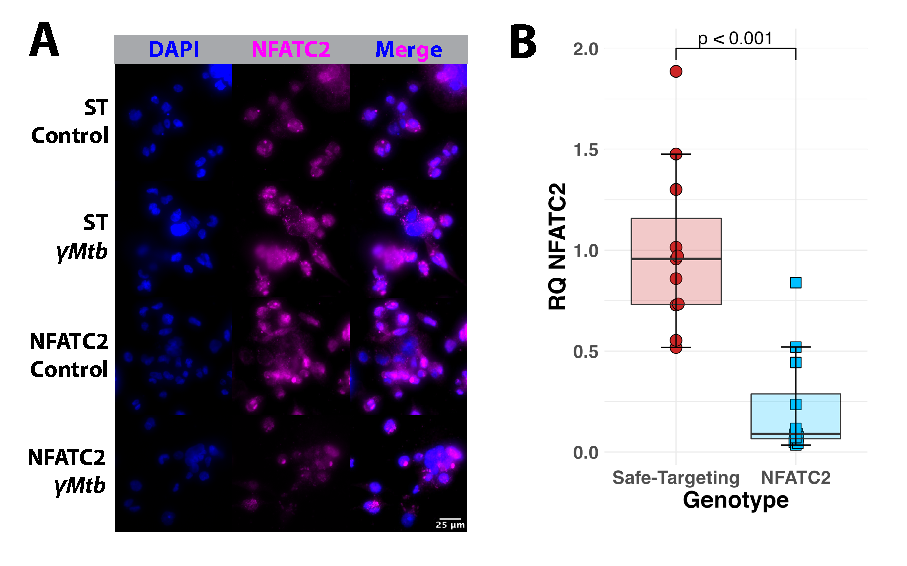
\includegraphics[height=3in]{images/lentivalid.pdf}
\caption{Validation of the lentivirus\hyp{}mediated knockout approach. (A) shows aberrant localization of NFATC2, suggesting that the remaining protein has been functionally disrupted. Note that the antibody binding site is N\hyp{}terminal to the sgRNA sites, a technical oversight in this design that made it difficult to quantify reductions in NFATC2 protein levels after targeting. (B) Nonsense\hyp{}mediated mRNA decay in suspension THP\hyp{}1 monocytes is reduced by NFATC2 targeting relative to safe targeting controls.}
% Provide a label so we can cross\hyp{}reference it from the tex
\label{figure:validation}
\end{figure}

\begin{figure}
\centering
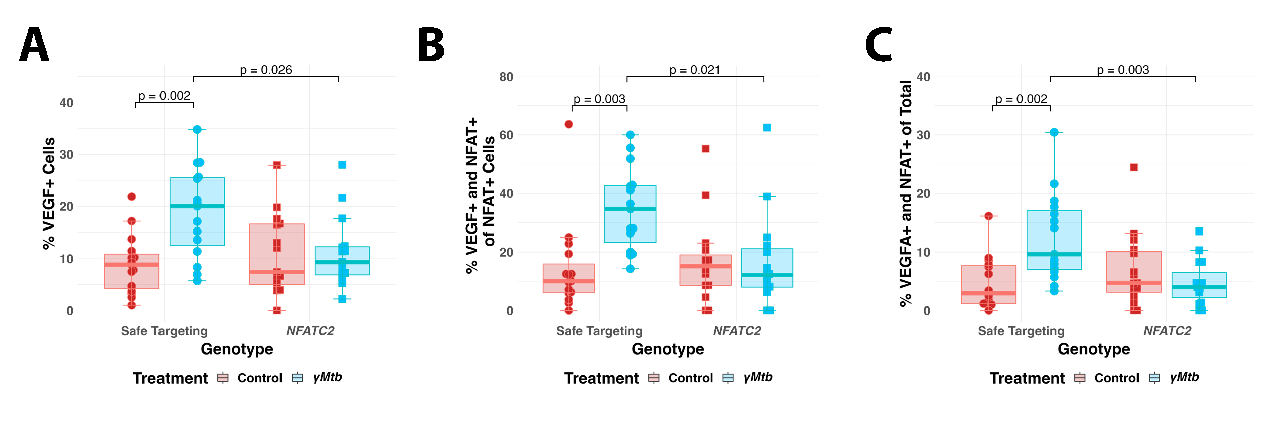
\includegraphics[width=\textwidth]{images/lentiIFquant.pdf}
\caption{Blinded quantification of our lentivirus\hyp{}transduced CRISPR/Cas9 THP\hyp{}1 macrophages demonstrating a reduction in the degree of VEGFA expression that corresponds to reduced NFATC2 nuclear responsiveness to $\upgamma$\textit{Mtb}. (A) shows the total percentage of VEGFA+ cells out of the total cells present. (B) is the percentage of cells with both VEGFA expression and NFATC2 nuclear translocation out of the total number of cells with NFATC2 nuclear translocation. (C) shows the percentage of the total number of cells that have both VEGFA expression and NFATC2 nuclear translocation. Together these data implicate NFATC2 in mediating the VEGFA response to $\upgamma$\textit{Mtb} exposure.}
% Provide a label so we can cross\hyp{}reference it from the tex
\label{figure:lentiIFquant}
\end{figure}

\section{Discussion}\label{pap:disc}

This work uncovers an unexpected and novel role for macrophage NFAT activation in immune responses to pathogenic mycobacteria and the maladaptive angiogenic responses that occur during infection. This activation of NFAT is driven through recognition of bacterial cis\hyp{}cyclopropanated trehalose 6\hyp{}6'\hyp{}dimycolate, a major constituent of the cell envelope in pathogenic mycobacteria, that we have previously found is necessary and sufficient to drive pathological angiogenesis (Walton et al., 2018). Identifying this unexpected role for NFAT in angiogenesis expands our understanding of the mechanisms governing mycobacterial pathogenesis and offers targets for potential host directed therapeutics. Traditionally, work on TDM\hyp{}mediated C\hyp{}type lectin activation has focused on CARD9 and NF\hyp{}$\upkappa$B signaling. Here, by contrast, we describe a specific role for alternative C\hyp{}type lectin signaling responses through the NFAT pathway to drive VEGFA production and granuloma\hyp{}associated angiogenesis. 

VEGFA induction is a prominent feature of tuberculosis in human disease as well as in a number of animal models, including non\hyp{}human primates, rabbits, mice, and zebrafish \citep{Datta2015, Oehlers2015, Polena2016, Harding2019, Cronan2021, Gideon2022}. We found that VEGF was produced specifically within newly arrived macrophages at nascent granulomas. Macrophage populations are critical to VEGF induction, as macrophage\hyp{}specific inhibition of NFAT signaling as well as deletion of \textit{nfatc2a} result in reductions in granuloma\hyp{}associated angiogenesis. Using a human cell culture model, we found that NFATC2 was similarly engaged in human cells as amongst all NFAT isoforms, only NFATC2 underwent robust nuclear translocation in response to \textit{M. tuberculosis} stimulation. Correspondingly, pharmacological inhibition of NFAT signaling in human cell culture as well as genetic inhibition of \textit{NFATC2} resulted in reduced VEGFA production.

Although animal models of tuberculosis generally report high VEGF levels, there are few studies that center on VEGFA induction in cell culture infection models. Through high\hyp{}resolution time\hyp{}lapses and reporter lines, we found that \textit{vegfaa} induction generally does not occur until the formation of initial granulomas and is generally correlated with the appearance of extracellular bacteria that could be recognized by incoming, likely uninfected macrophages. This concentration\hyp{}dependent effect on signaling may reflect key aspects of the disease itself, wherein large masses of extracellular bacteria accumulate in the necrotic core of the granuloma, potentially triggering relatively insensitive and/or chronic C\hyp{}type lectin signaling in this context. Given what is already known about the need for chronic stimulus to produce effective NFATC2 activation, this would coherently fit with existing models and would offer a mechanism wherein other NFAT isoforms could play other roles earlier in infection but NFATC2 is specific to later stages at high intensity and duration of activation \citep{Yissachar2013, Kar2015}. 

Consistent with the recognition of extracellular bacteria, exposure of human macrophage\hyp{}like cells to $\upgamma$\hyp{}irradiated M. tuberculosis rapidly induced NFATC2\hyp{}dependent VEGF signaling in a dose dependent manner. Standard cell culture infection models generally eliminate extracellular bacteria using gentamicin treatment and media changes, and so it is possible that engagement of this pathway by extracellular bacteria or TDM stimulation is a key component of this response. A survey of the literature and a variety \citep{Lee2019, Pisu2020, Hall2021, Looney2021, Pu2021} of RNA\hyp{}seq datasets from macrophage\hyp{}\textit{M. tuberculosis} infection experiments reveal modest or nonexistent induction of VEGFA, further supporting the notion that extracellular exposure to \textit{M. tuberculosis} may be an important element of the angiogenic response and may reflect some aspects of the macrophage\hyp{}\textit{M. tuberculosis} interface within granulomas \citep{Orme2014b}.

As its name suggests, the NFAT pathway plays an indispensable role in normal T cell biology. Accordingly, whole animal knockouts of NFAT in standard mouse models of \textit{M. tuberculosis} infection --€“ where granuloma formation itself may be limited --€“ may have obscured a role for myeloid\hyp{}specific effects of NFAT signaling \citep{Via2012}. This study investigated a role for NFATC2 in control of \textit{M. tuberculosis} infection and found that NFATC2 was required for effective bacterial control and production of TNF\hyp{}$\upalpha$ and IFN\hyp{}$\upgamma$ in CD4\textsuperscript{+} T cells despite no perturbation of the expression of these genes in dendritic cells, suggesting an adaptive immune response\hyp{}specific defect in bacterial control. This may be of little surprise, given the extensive contacts that T cells have with mycobacteria within the lesions that develop in standard mouse models. Such a defect in T cell responses may be important for bacterial control when T cells are able to access the bacteria, but this condition is not reflective of the biology of the granuloma in other models or humans. It would be interesting to explore the phenotype of a \textit{LysM\hyp{}Cre}; \textit{Nfatc2\textsuperscript{fl/fl}} mouse infected with tuberculosis to isolate the macrophage\hyp{}dependent phenotypes. However, given our findings on macrophage NFAT contributions to angiogenesis, which is poorly modeled in the mouse, either entirely new roles for NFAT may be uncovered or it may have little or no effect on bacterial growth and disease. In any case, the present results offer some tension with these historical findings and it may take additional work to definitively identify any role for NFATC2 in the overall pathogenesis of tuberculosis infection.

The zebrafish model, by looking at early timepoints, uncovered a role both in angiogenesis and, presumably as a consequence, bacterial control. Wholesale, longer\hyp{}term inactivation of NFAT, which also plays important roles in T cells, would potentially compromise important aspects of a productive adaptive immune response during mycobacterial infection. While genetically manipulable animal models allow for cell\hyp{}specific separation, any host\hyp{}based therapeutic approaches might require cell\hyp{}specific macrophage delivery methods \citep{Hu2019, Mukhtar2020, Colombo2022}, NFATC2\hyp{}specific targeting \citep{Kitamura2021}, and/or contend with the adaptive immune response\footnote{Although NFATC2 appears to be largely redundant with both NFATC1 and NFATC2 for many, but not all adaptive responses, it is still important to, as specifically as possible, target the desired pathway for minimal off\hyp{}target side effects.}, an important aspect of host resistance during mycobacterial infection.

While little else has been studied in the context of NFAT\hyp{}mycobacterial interactions, a previous publication assessed the contributions calcineurin activation on the mycobactericidal activity of macrophages and found that mycobacteria manipulate an actin\hyp{}binding protein called Coronin\hyp{}1 to block phagosomal\hyp{}lysosomal fusion and do so by activating calcineurin \citep{Jayachandran2007}. In the absence of Coronin\hyp{}1 or after treatment with calcineurin inhibitors, lysosomes efficiently fused with the mycobacteria\hyp{}containing phagosomes, mediating bacterial killing. This effect was found to be independent of transcription, implicating calcineurin in somehow modulating the process of phagosomal\hyp{}lysosomal fusion, potentially through some interaction with Coronin\hyp{}1 and actin. However, a subsequent publication found that this process was independent of actin \citep{Jayachandran2008}, leaving it a yet\hyp{}to\hyp{}be resolved mystery how directly calcineurin\hyp{}dependent activity blocks phagosomal\hyp{}lysosomal fusion to facilitate mycobacterial survival and replication. If nothing else, this adds to the body of evidence suggesting that calcineurin/NFAT\hyp{}based host directed therapies may have multiple modes of host\hyp{}beneficial activity.

It remains unclear why NFATC2, but not any of the other isoforms, is specifically required in macrophages for the induction of VEGFA, given evidence that the others are present in resting macrophages (\autoref{figure:isoforms}). The functional distinctions between the isoforms have long been of basic interest, but relatively few specific differences between them have been identified beyond basal regulation to provide tissue\hyp{}specificity and more recent findings describing layers of kinetic regulation with isoform\hyp{}specific stimulation thresholds, nuclear retention, and more \citep{Lyakh1997, Rao1997, Kar2014, Kar2015, Kar2016, Yissachar2013}. Anecdotally, we observed substantially higher expression of NFATC2 by immunofluorescence after $\upgamma$\textit{Mtb} exposure even with INCA\hyp{}6 treatment, suggesting that there may be interesting upstream regulatory mechanisms, potentially dependent on HIF\hyp{}1$\upalpha$ or NF\hyp{}$\upkappa$B. These novel levels of regulation offer opportunities for uncovering new features of the cell biology of NFAT.

NFAT is also likely to be involved in modulating the expression of other important pro\hyp{}angiogenic chemokines, including CXCL12, the primary ligand for CXCR4. CXCR4 has been previously demonstrated to be critical for granuloma formation and angiogenesis \citep{Torraca2017} and NFAT has been shown to be able to regulate CXCL12 expression, at least in osteoblasts \citep{Sesler2013}. It may be reasonable to think that NFATC2 is also mediating CXCL12 expression during infection and is acting as a more central regulator of angiogenic responses. This hypothesis warrants further study; in any case, the stimulus for and transcriptional mediators of the observed CXCR4\hyp{}dependent granuloma angiogenesis should be identified to add to our understanding of how these processes occur.

\begin{figure}
\centering
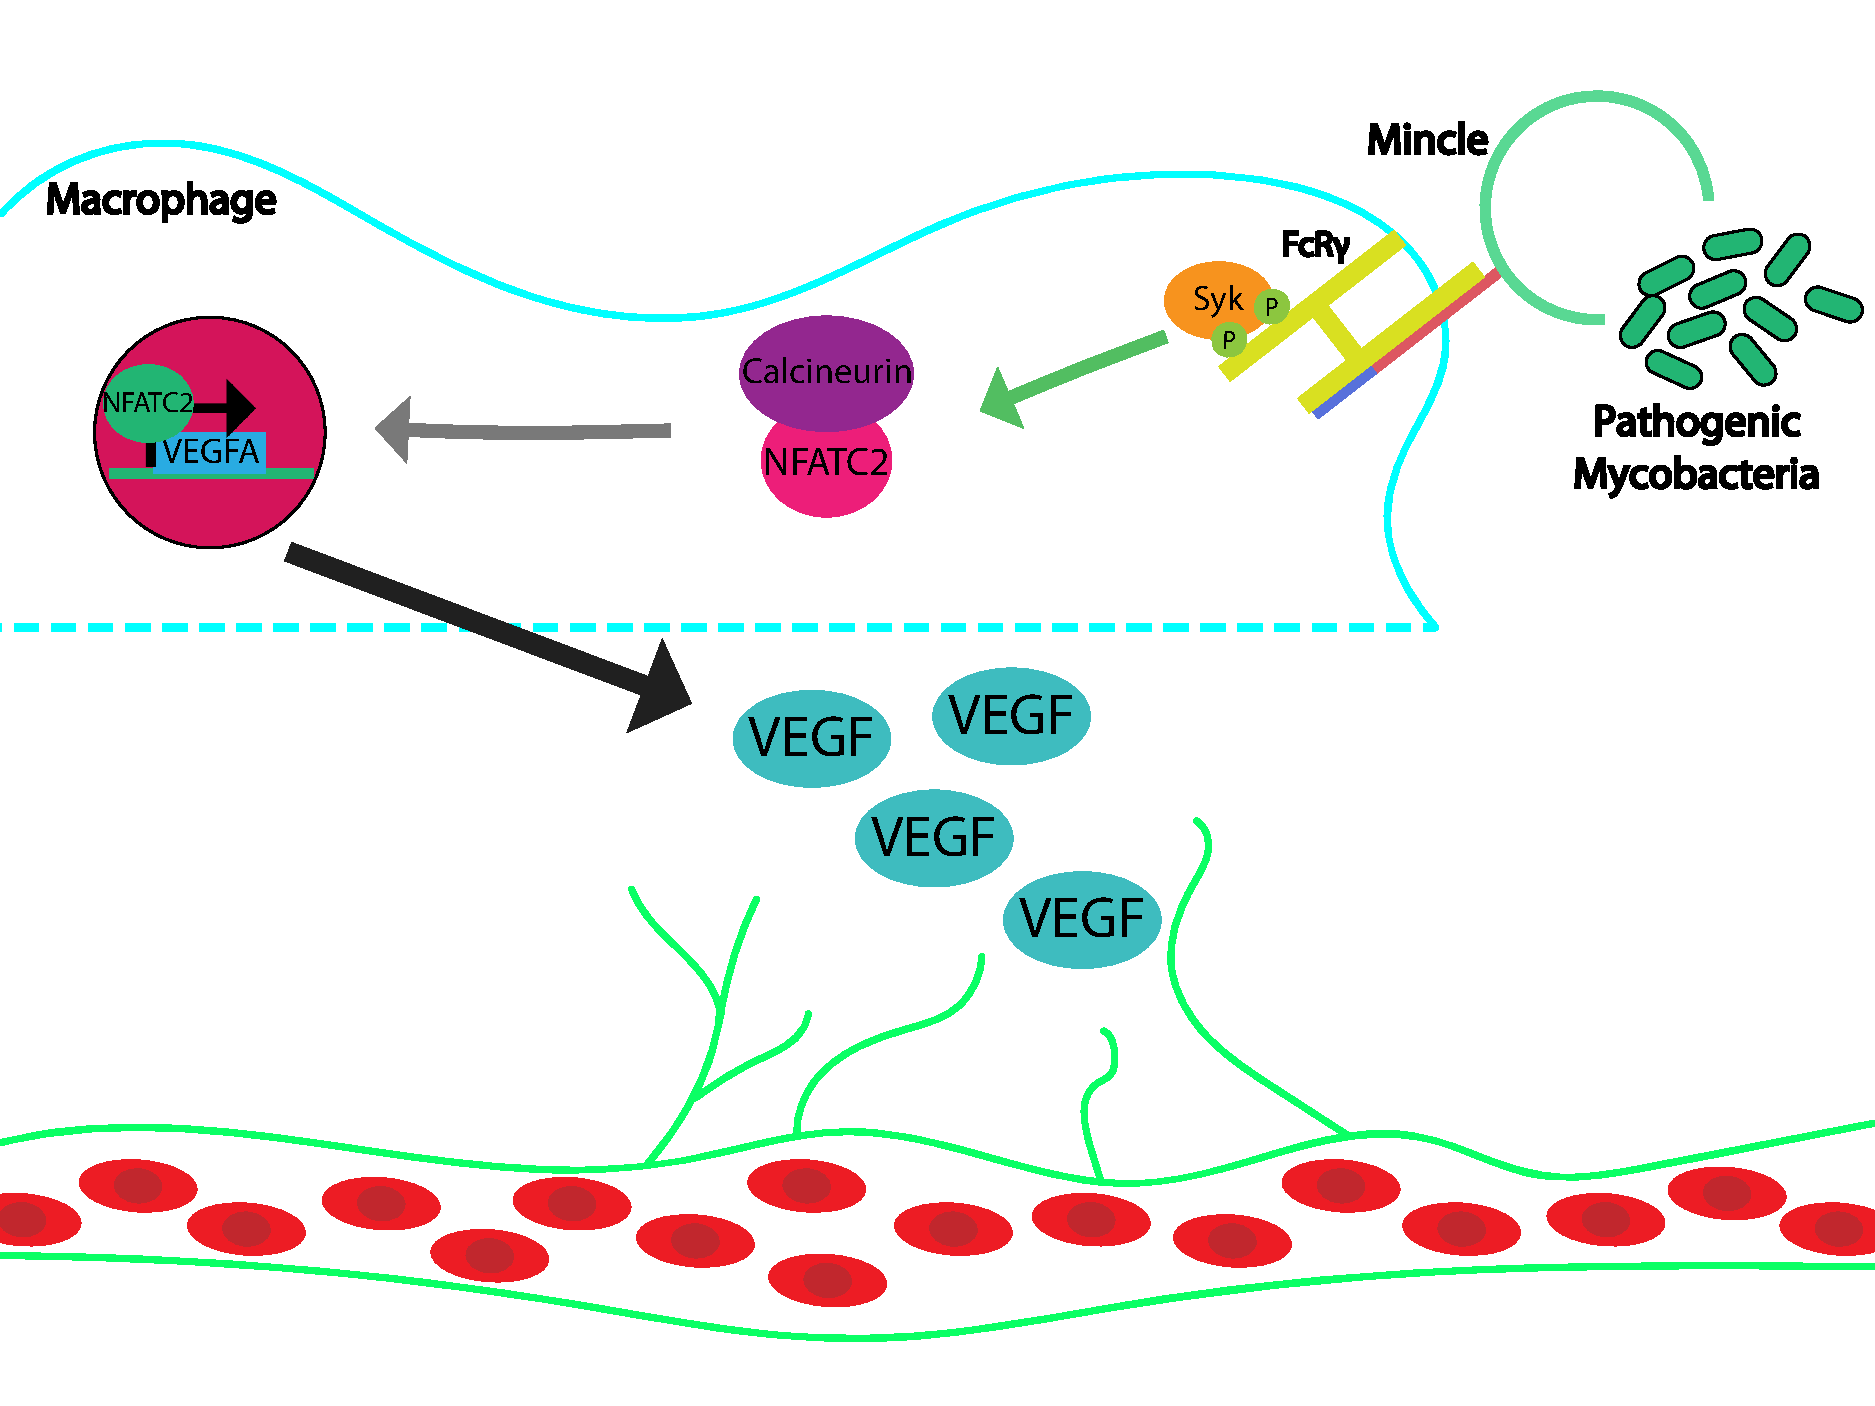
\includegraphics[width=\textwidth]{images/conclusion_schematic.pdf}
\caption{Upon completion of this work, we have identified a critical role for NFATC2 activation downstream of TDM detection in mediating the production of VEGFA by macrophages, which induces angiogenesis. This clarifies a major question in the field as to the underlying mechanisms of angiogenesis and opens new paths for investigation into the contributions of the NFAT signaling pathway to mycobacterial pathogenesis.}
% Provide a label so we can cross\hyp{}reference it from the tex
\label{figure:endschematic}
\end{figure}

Here, we identify the unique requirement for this single isoform in macrophages to induce angiogenesis in response to mycobacterial infection (\autoref{figure:endschematic}). One hypothesis is that NFATC2 has binding partner(s) unique among NFAT isoforms required for its effect on the VEGFA promoter. Whether this is HIF\hyp{}1$\upalpha$ (the canonical regulator of VEGFA) or one of the many previously described interacting partners is, as yet, unknown, but could be tested either \textit{in vitro} or \textit{in vivo} with genetic or chemical approaches (\autoref{hifnfat}). However, higher order regulatory mechanisms that result in the production of VEGF in the absence of overt hypoxia have been understudied and this work proposes at least one potentially generalizable mechanism whereby NFATC2 activation results in VEGFA transcriptional upregulation, a process that can be inhibited with chemical and genetic intervention. Despite the widespread presence of putative NFAT binding motifs (5'€™\hyp{}GGAAA\hyp{}3'€™) (\autoref{figure:promoter}) in the proximal VEGFA promoter \citep{Gearing2019}, their influence on VEGFA transcription has been relatively unexplored as this specific effect is generally not seen in T cells or other cell types \citep{Chang2004}. This single publication from \citet{Chang2004} found that the \hyp{}2400 site in the \textit{VEGFA} promoter was specifically bound by NFATC proteins and acted to \textit{repress} transcription. This is an intriguing hypothesis that might suggest that NFAT is able to repress \textit{VEGFA} transcription at baseline but may act to induce it after stimulation. Such results would be consistent with the mild but reproducible increase in VEGFA we observe with INCA\hyp{}6 treatment in our experiments in THP\hyp{}1 cells (\autoref{figure:qpcr}). 

As described in \autoref{NFAT}, NFAT is involved in the induction of a variety of cytokines including IFN\hyp{}$\upgamma$ and TNF\hyp{}$\upalpha$, but whether NFAT\hyp{}dependent transcriptional induction of these within macrophages has a role in the overall course of disease is unknown. This surely offers promise for the future as an expansion of the present work to incorporate a more complete view of the NFAT\hyp{}dependent signals that influence mycobacterial disease progression.

\begin{figure}
\centering
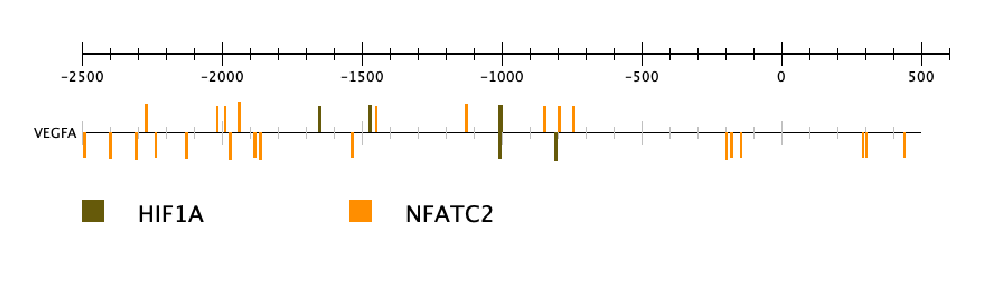
\includegraphics[width=\textwidth]{images/vegfapromoter.pdf}
\caption{NFATC2 and HIF\hyp{}1$\upalpha$ putative binding sites in the VEGFA promoter as determined by CiiiDER. There are several NFAT binding sites in the promoter, the function of which has largely yet to be determined.}
% Provide a label so we can cross\hyp{}reference it from the tex
\label{figure:promoter}
\end{figure}

A more comprehensive characterization of NFAT\hyp{}dependent innate immune responses has begun in recent years \citep{Deerhake2021, Peuker2022, Poli2022} (for a more detailed description, see \autoref{nouveaunfat}), but this pathway has remained unstudied in the context of macrophage signaling during mycobacterial infection. Furthermore, this work draws a connection between the induction of calcium fluctuations --€“ which can occur in response to many different developmental, homeostatic, and pathological stimuli, including to mycobacterial infection \citep{Kusner2001, Jayachandran2007, Jayachandran2008, Matty2019, Malik2000} --€“ to the angiogenic response to that stimulation. Our identification of NFAT regulation of VEGFA offers a novel approach to both pro\hyp{} and anti\hyp{}angiogenic intervention in various pathological contexts.

\subsection{Limitations of the Study}

The limitations of this study, like all studies, are innumerable. While I am proud of what I have accomplished in pursuit of this work, there are many opportunities for the future as well as further work to clarify the results we have found here. We have identified interesting macrophage biology mediating an important disease\hyp{}relevant phenotype during mycobacterial infection, but we do not see the same magnitude of bacterial burden change as with VEGF\hyp{}inhibition alone \citep{Oehlers2015}, suggesting pleiotropy in the NFAT signaling pathway with inhibition resulting in both pro\hyp{} and anti\hyp{}bacterial effects. What these antimycobacterial aspects of NFAT signaling are is worth investigation to better understand the full corpus of possible consequences to NFAT inhibition strategies for the treatment of infectious disease and the potential risks for patients already taking calcineurin inhibitors. To do so, RNA\hyp{}seq or similar should be employed to better delineate these alterations in gene expression profile. It would also be beneficial to work toward disentangling some of the other effects of NFAT inhibition by simultaneous treatment of the zebrafish with VEGFR2 inhibitors in the \textit{irg1}:\textit{VIVIT} background to directly test non\hyp{}angiogenic features of NFAT in mycobacterial infection.

We have thus far been unable to identify the particular macrophage receptor responsible for detecting TDM in the zebrafish. While work in THP\hyp{}1 macrophages may be able to more affirmatively link MINCLE or MCL to the activation of NFAT, identification of the zebrafish receptor would make a substantive contribution to model development as well as the evolution of C\hyp{}type lectin receptors more broadly. Cell\hyp{}type specific knockout of \textit{nfatc2a} would also aid greatly in definitively linking this gene to VEGFA induction and angiogenesis, but the tools to do so are not yet operational; perhaps future studies can begin with such intent and focus more stringently on the role of this isoform strictly in macrophages.

Some technical limitations are also interfering with interpretation of some results. Generation of stable knockouts of NFATC2 in THP\hyp{}1 macrophages would make for more robust and cleaner assays, although it has the limitation of odd clonal behavior and loses the heterogeneity that can be advantageous in dissecting some phenotypes. The variable ploidy of these cells is also a challenge, so an alternative macrophage model or primary cells may be required to more effectively model some of these responses.

This macrophage\hyp{}NFAT signaling pathway likely has important roles in other disease contexts that are not addressed here. Tuberculosis is the most common cause of granuloma formation, but it is far from the only cause, and any contributions of this pathway to granuloma biology in \textit{Schistosoma}, \textit{Cryptococcus}, or \textit{Histoplasma} infections is not yet known. However, with the tools now available, these roles are likely to be easier to study in the future and new insights may be gleaned from such investigation. Angiogenesis is a common pathology in some autoimmune diseases, such as arthritis, and is prevalent among cancers; whether macrophage NFAT signaling might be mediating angiogenesis in these contexts is surely of future interest and may reveal novel aspects of the host\hyp{}tumor interface.

We have validated important aspects of our observations in the zebrafish with a mammalian cell culture model, but subsequent studies may warrant further integration of mammalian models of tuberculosis infection where angiogenesis is present (rabbits, guinea pigs, macaques) or human patient samples to better understand certain aspects of the underlying biology and validate NFAT induction during tuberculosis infection and potential correspondence to VEGFA production.


\end{doublespace}

\chapter{Novel Computational Approaches to Image Processing and Quantitation}\label{chap4}

\begin{doublespace}
High-resolution, high-throughput microscopy has opened possibilities for biological analysis that were inconceivable only a few short years ago, but the methods by which to analyze these data remain largely lacking. While heroic efforts have been made to use both standard thresholding methods as well as newer machine learning-powered methods to simplify and automate image processing, these approaches are often somewhat limited by the range of purposes for which they were designed and tested. While the open source nature of many of these approaches facilitates adaptation, this is both technically beyond the skillset of many scientists and impeded by, at best, variable quality documentation. Additionally, many of the tasks that experimenters seek to do are both relatively simple and highly repetitive but they are often unaware of the means by which to cut down on manual processing time in order to economize their time and energies. These scripts are a combination of automation scripts that will process particular image types into smaller and more informative images (compression of Z-stacks, time-series, etc.) and those meant for analysis of image data (pixel intensity distribution across an image, bacterial burden within larval zebrafish). While none of these are of the caliber to open entirely new methods of analysis, I hope they are a catalyst for others in the zebrafish community at large to explore the potential for computational automation to save time and frustration in the process of analyzing often thousands of very large, data-rich images.

All of the scripts in their latest versions will be able to be found in perpetuity at \url{http://github.com/jaredbrewer/image-analysis}. A static version of these has been created at Zenodo (\url{https://doi.org/10.5281/zenodo.7036029}). Scripts at the end for RNA sequencing analysis are available at Zenodo (\url{https://doi.org/10.5281/zenodo.6981721}). 

\section{FIJI/ImageJ}\label{fiji}

ImageJ was first developed in embryo in the 1980s as a means of viewing scientific images on the Mac, but matured into the program we know today in the 1990s when it was ported to Java. The original ImageJ1 is still developed and maintained today and serves as the foundation of its functional successor, FIJI. \underline{F}iji \underline{I}s \underline{J}ust \underline{I}mageJ is essentially ImageJ2 bundled with a set of useful plugins that aid in visualizing and analyzing scientific imaging data. Preeminent among these bundled plugins is a library of programming languages that can be used to interface with the underlying Java-based APIs that make FIJI function. Among the options, Python is likely the most widely known and written programming language among biologists and this opens up a great deal of potential for object-oriented programming centered on the analysis of images. 

The default language in ImageJ, the ImageJ1 Macro language (.ijm), is approximately based around Java but lacks defined sets of methods (for most purposes) and objectification, has difficulty with interfacing with file systems, and exposes a great deal of underlying computer logic to the user. Take, for instance, the procedure for writing a \textit{for} loop:

\begin{code}
\begin{minted}{java}
for (i = 0; i < 10; i++) {
    print("Hello");
}
\end{minted}
\end{code}

\begin{code}
\begin{minted}{python}
for i in range(1:10):
    print("Hello")
\end{minted}
\end{code}

The former example, written in the IJ1 macro language, exposes the user to looping over a set of indices from 0 to 10 and incrementing with each loop, uses curly braces to define the boundaries of the loop block, and requires each line to end with a semicolon. These are all standards features of many popular programming languages, but for FIJI, the key is to be as legible of a programming language as possible since the writers of most of these macros are \textit{not} software engineers. Python, by contrast, increments for the user and will increment through an entire set of objects without needing to know how many objects are present. Blocks of code are delimited by spaces or tabs, so the relative location of the code on the line is informative as to what it relates to. Additionally, Python has well-studied and well-defined object types with specific associated methods that translate between all versions of Python. The benefits of the Python community only add to the value proposition of learning and using Python both generally and within ImageJ.

Not only this, but to loop through directories of files, the ImageJ macro language struggles even further, with little awareness of file structures or regular expressions whereas Python can trivially fetch lists of files by user-defined patterns from mixed directories and even search through subdirectories recursively.
 
\section{Python}\label{python}

As alluded to, Python is a dynamically typed high-level programming language that is widely used for generating automation scripts of all varieties in addition to web server backend applications, data science, and even game creation \citep{vanRossum1995}. The advantages of Python are derived from the enormous community of developers who use Python and who continue to develop it as a language. In data science, the utility of pandas and numpy are unmatched and these alone make Python a language worth learning for any molecular biologist in the analysis of their quantitative data. Throughout this work, I have used Python both within the FIJI/ImageJ interpreter (which is based on Jython version 2.7.2) and via CPython 3.11, the standard distribution of Python, in the Terminal. While Jython is nominally different from standard Python, when written appropriately, it is simple enough to write version-universal code within the relatively narrow confines of what I have sought to accomplish thus far with it.

One of the key developments in the field of FIJI and Python is the release of PyImageJ, a complete API interface between CPython and ImageJ2, written in Python \citep{Rueden2022}. Going forward, it will be useful to reimagine some of these scripts and approaches to utilize the PyImageJ-defined API, as this is clearly the future of scripting in FIJI. Use of the image viewer in an \textit{ad hoc} fashion is likely superior to an image-first approach for many tasks and PyImageJ cuts a lot of the unfortunate overhead from the graphical elements of FIJI. Unfortunately, such a translation is nontrivial as the command structure and imports have changed quite dramatically and in ways that are not as well documented as the base API. However, such an implementation allows FIJI/ImageJ to make use of pandas, numpy, and OpenCV in Python, making for a more complete data science package and streamlining data collection and processing in a single language. 

\subsection{Napari}

While FIJI/ImageJ have served as the key to the analyses presented both here and in \autoref{chap3}, it is not the only image analysis software available. An alternative, written in pure Python, is napari, which is in the middle stages of alpha testing as of this writing \citep{napari}. While not yet feature complete, it is a lightweight alternative to FIJI and, with proper optimization, can likely outperform FIJI in the long run. By shedding dependence on Java, memory management and performance are able to be improved while the lowest-level image processing can be done in C invisible to the end user. At the present time, however, FIJI seems to be the most robust and widely accepted option and will likely remain so for the conceivable future. A bridging option, \textit{napari\hyp{}imagej} is in the works and promises to dramatically expand the napari feature set, but does not aid in napari independence from Java or older modalities.

\section{R}\label{R}

As previously detailed (\autoref{meth:R}), R is a convenient and easy-to-learn object-oriented statistical programming language. This language has made a monumental contribution to data science and is used extensively throughout this work to analyze and visualize the resulting datasets. While less extensively used in this segment than Python, it is key to a lot of further analyses and is exhaustively used for all of the visualization seen in \autoref{chap3}. Many of these same functions can be executed in Python, but I attempt to utilize the best tool for a given task at a given time and R is often the best, most flexible way to work with arrays and data frames.

\section{Maximum-Intensity Projection and Composite Image Generation}\label{mippers}

The fundamental premise of the ImageJ macro system is to simplify repetitive tasks to free up user time for higher forms of analysis and the default language (the ImageJ1 macro language) makes it easy to write procedural operations to be done on single images, but is difficult to scale to whole directories of images or accept various types of user input. I have thus developed a set of scripts that allow the user to rapidly generate maximum-intensity projections from sets of images and then generate composite images. This often condenses hundreds of megabytes of data into $<$30 MB, makes for more flexible image viewing and understanding, and allows the images to be opened in essentially any number (many hundreds to thousands) on any personal computer. These procedures are also internally memory managed, allowing them to run on most personal computers indefinitely to process the sometimes thousands or tens of thousands of images that can be generated over the course of an experiment with multiple wavelengths, Z stacks, XY positions, and times\footnote{If you have 4 channels across 48 stage positions, capturing every 30 minutes for 48 hours, you would have 18,432 individual images based on Metamorph's file saving structure; this can clearly get out of hand very quickly.}. In our lab, we primarily use output files from epifluorescent Zeiss microscopes, which generate .czi files and from Metamorph connected to a custom spinning disk confocal system, which generates .tiff files.

The maximum intensity projection is an extremely common way of condensing multidimensional images into a single two-dimension representation by finding the brightest pixel at every XY position and accepting it as the most ``in focus'' pixel. The success of this depends on images being properly exposed, but in most instances will generate a reasonably sharp image ready to be quantitated or presented. In any case, data spanning multiple Z stacks requires some degree of integration to be usefully presented to others or manual scanning through libraries of hundreds of images and these pipelines will facilitate that type of visualization at scale.

\begin{code}
\caption{This script allows the user to open as many files as their memory allotment will allow and then to Z project them one at a time with custom start and end positions. This ability often generates cleaner, sharper images by individually selecting the lowest and highest in-focus frames, but necessarily takes more time than a more automated approach.}
\label{slowmanmip}

\inputminted[breaklines,frame=single,fontsize=\small]{python}{source/manMIPper.py}

\end{code}

The use of \autoref{slowmanmip} is to process a set of already opened images and generate maximum intensity projections from these and, optionally, save them back into the directory that they came from. This relatively simple set of GUI-guided processes allows the user to, in two clicks, accomplish a task that previously would have required a great deal of menuing to accomplish. The goal is narrow, but this execution is extremely useful when working through large numbers of images.

\begin{code}
\caption{A low overhead version of the manual maximum intensity projection script described above. Instead of opening all of the images first and then running the script, the script will processively open unanalyzed images one at a time and periodically garbage collect, allowing for entire directories to be processed at once on most reasonably modern computers.}
\label{fastmanmip}

\inputminted[breaklines,frame=single,fontsize=\small]{python}{source/fast_manMIPper.py}

\end{code}

\autoref{fastmanmip}, while not always the correct choice depending on user preferences and system capabilities, is much less memory hungry than the original version above, but typically results in slightly slower overall operations due to the delay in opening images. If the images are on fast internal storage, then this is certain to be faster than \autoref{slowmanmip}, but when reading from external storage, the I/O limitations will likely make it faster to open all of the images prior to processing unless system memory is severely limited. Nevertheless, the nature of this makes it very generally useful on older systems.

\begin{code}
\caption{This script can be used in instances where the first and last stacks of a desired Z projection span the entire set of stacks provided. It will process an entire directory of images together and output the result into a subdirectory of the original.}
\label{bulkmip}

\inputminted[breaklines,frame=single,fontsize=\small]{python}{source/bulkMIPper.py}

\end{code}

While the previous scripts have expected user input for each image, the skilled microscopist can select top and bottom slices that will suffice for generating Z projections during imaging itself. This means that the first and last slices of the projection are typically the first and last slices of the images \textit{in toto}. This script takes a directory of images as an input and will perform total maximum intensity projections on all of them and save in a new subdirectory. After observation, any that seem incorrect can then be processed with one of the preceding scripts, especially \autoref{slowmanmip}. 

\begin{code}
\caption{An interface to functions allowing slices in a Z-stack to be kept or removed as desired through function calls. This can integrate into other workflows and be connected to the previous scripts through higher-order wrappers.}
\label{reslicer}

\inputminted[breaklines,frame=single,fontsize=\small]{python}{source/reSlicer.py}

\end{code}

FIJI/ImageJ comes with a built-in option to keep and remove particular slices, but the native plugin does not readily fit into object-oriented programming pipelines like those used by Python and Java. Thus, I have adapted the underlying logic of these plugins to be wrapped in various other scripts through calls to the defined functions, \textit{sliceKeeper} and \textit{sliceRemover}. For instance, this allows calls to the maximum intensity projection plugins to be funneled into this plugin to simultaneously generate the kept slices as well as the maximum intensity projection of those kept slices for some useful improvements to data integrity. 

\section[Surface Plot Analysis for Cellular Distribution of Labeled Proteins]{Surface Plot Analysis for Cellular Distribution of Labeled Proteins\footnote{Taken from personal contributions to \citet{Saelens2022}.}}

The distribution of a protein across the cell body can indicate changes in function of the protein and alterations in cell behavior, but analysis of such changes is not quite trivial. There are methods for drawing lines and plotting fluorescence intensity, but this fails to integrate the entire cell in three dimensions in to the analysis as it proves to be only one dimensional along that line. To analyze the distribution of ARPC2 in BLaER1 macrophages during \textit{M. tuberculosis} infection, I developed a novel analysis pipeline that integrated the 3D Surface Plot plugin of ImageJ. This pipeline takes a raw image, isolates the desired channel, opens it in 3D Surface Plot for visualization, and then takes the user-generated output of 3D Surface Plot to find the maximum fluorescence along the longest axis of the cell. As this analysis is designed for macrophages, which can develop long spindles, this allows for quantitative proximal/distal differences in the localization of a protein to be determined.

\begin{code}
\caption{A script to isolate a single cell within a frame.}
\label{isolator}

\inputminted[breaklines,frame=single,fontsize=\small]{python}{source/autoIsolator.py}

\end{code}

The first step of this pipeline is to isolate the cell using some reference channel, which can also be the channel you are measuring if necessary, although I would recommend using some sort of pan-cytosolic or plasma membrane marker to more thoroughly mark the outline of the cell and to use that instead. The script presents a simple GUI and allows the user to select the needed parameters and will then process entire folders of images into isolated cells in a single channel. A missing feature is that it needs to be able to isolate each cell from images that contain more than one cell, to save the user time on isolating cells in their own separate files by hand. This could conceivably be done by integrating logic around coping ROI contents into new images, but that is a work-in-progress at this time.

The output is a folder of single-channel files ready to be input into 3D Surface Plot, which can be launched with the following:

\begin{code}
\begin{minted}{python}
from ij import IJ, ImagePlus

imp = IJ.getImage()

IJ.run(imp, "3D Surface Plot", 
    '''plotType=1 
    colorType=3 
    drawAxes=0 
    drawLines=0 
    drawText=0 
    grid=256 
    drawLegend=0 
    smooth=8.5 
    backgroundColor=000000 
    windowHeight=600 
    windowWidth=720''')
\end{minted}
\end{code}

The image then needs to be rotated until it is along its longest axis in XY and then oriented precisely perpendicular in XZ (this can be done by turning the axes back on temporarily, although they must be turned off before the next step). This will give the longest two dimensional axis of the image and show a series of peaks and valleys corresponding to a smoothed-over rendition of the image. This can then be exported and, if desired, saved using:

\begin{code}
\begin{minted}{python}
from ij import IJ, ImagePlus
from os import path

outputdir = "" # Insert save directory as a string.
imp = IJ.getImage()
title = imp.getTitle()

out = path.join(outputdir, title)
IJ.saveAs(imp, "Tiff", out)
\end{minted}
\end{code}

I recommend saving them for reference later, as the quantitation can occasionally be bugged by strange smoothing, etc. Any outliers will need to be inspected by hand and saving the intermediates can help a great deal with that. Additionally, saving allows further automation in the next step (although, as we will see, automating across all open images is also now possible and will be built into these options in the future).

\begin{code}
\caption{A script to automatically capture the signal at each point along an image and save it to a CSV file.}
\label{surfaceplot}

\inputminted[breaklines,frame=single,fontsize=\small]{python}{source/autoSurfacePlotMeasure.py}

\end{code}

This script is key to capturing the points along the abstracted profile of the cell. It is relatively simple in that it just writes to a CSV each XY coordinate where there is a signal, which can then be condensed by finding the maximum point at each X position in R, which is the final step in the analysis.

\begin{code}
\caption{A script to conduct computational filename blinding from the command line written in Python.}
\label{blinder}

\inputminted[breaklines,frame=single,fontsize=\small]{r}{source/surface_plot_analysis.R}

\end{code}

This R script takes the CSV format output from FIJI/ImageJ and processes it by finding the maximum value along the curve and using that as the peak relative fluorescence intensity for that X position and then calculates the area under the curve across a defined interval. For instance, the middle 50\% of the cell can be defined as "central" and the outer 25\% can be defined is "distal" and these values normalized to one another and then compared across different experimental groups. It was found that BLaER1 cells infected with \textit{M. tuberculosis} expressing ancestral \textit{esxM} had less distal localization of ARPC2, suggesting that this bacterial effector was altering actin dynamics in these cells.

\section{py-LaRoMe}\label{larome}

The original purpose of LaRoMe (\url{https://github.com/BIOP/ijp-LaRoMe}) is to extract various features from images and is distributed as an ImageJ plugin. However, like many FIJI/ImageJ plugins, the design of LaRoMe is purely operational. In my attempts to utilize CellProfiler \citep{Carpenter2006, Kamentsky2011, McQuin2018, Stirling2021} to automate capture of various details about the THP-1 macrophages from \autoref{thp1inca} and \autoref{thp1lenti}, I wished to incorporate LaRoMe into Python pipelines to increase my throughput of analysis. This, however proved challenging based on the original design of the plugins, as they did not accept an image as an argument and expected to use the currently active image window.

I therefore completely rewrote these plugins explicitly so that they would accept an image as the primary argument, which allows for easy integration into looping structures. In the process, the entire plugin was translated from Java to Python. It is hoped that in the future, these code bases can be reconciled so that the existing distribution of LaRoMe, managed by BIOP, can incorporate both the excellent GUI options already existing and allow for interfacing through scripts for high-throughput applications.

\begin{code}
\caption{A Python translation of the FIJI function ``Label image to ROIs'' from LaRoMe. This function allows the user to take images generated from CellProfiler and convert them into a set of regions of interest in the ROI Manager.}
\label{l2r}

\inputminted[breaklines,frame=single,fontsize=\small]{python}{source/labelsToROIs.py}

\end{code}



\begin{code}
\caption{A Python translation of the FIJI function ``ROIs to label image'' from LaRoMe. This allows the user to use a set of ROIs to regenerate a label image, useful for creating masks on existing images and comparing areas between different channels.}
\label{r2l}

\inputminted[breaklines,frame=single,fontsize=\small]{python}{source/ROIsTolabels.py}

\end{code}



\begin{code}
\caption{A Python translation of the FIJI function ``ROIs to Measurement Image''. This combines the a defined set of ROIs (probably from labelsToROIs.py) and a raw image and generates an image that graphically represents measurements such as area or circularity.}
\label{r2m}

\inputminted[breaklines,frame=single,fontsize=\small]{python}{source/ROIsToMap.py}

\end{code}



\section[Experimental Blinding via a Single-Click Command Line Interface]{Experimental Blinding via a Single-Click Command Line Interface\footnote{Implementation from \citet{Brewer2022}, original conception from \citet{Salter2016}.}}\label{blinders}

\begin{code}
\caption{A script to conduct computational filename blinding from the command line written in Python.}
\label{blinder}

\inputminted[breaklines,frame=single,fontsize=\small]{python}{source/renamer.py}

\end{code}

In the process of data collection (especially image acquisition), the experimenter will typically assign each file a logical name indicative of what it contains. However, these file names are also a critical breakdown in analytical blinding and ways to avoid this are essential to prevent the introduction of excess experimenter bias into the process of analysis. This problem is clearly widespread, but solutions are difficult to come by. Individuals can have labmates or others to rename folders or files to obfuscate their contents, but this has the danger of the human element -- it would not be that difficult to lose track of any alterations and make subsequent quantitation worthless. Thus, a computationally robust method is required. 

\citet{Salter2016} saw this issue and elegantly addressed it through a Perl script \citep{Wall2000}. The author generated a script that would allow you to provide a single argument -- a folder -- and have the contents renamed and output a keyfile. This implementation was excellent and used throughout my work, but as time passed, I found it lacking in two major areas: recursion and the ability to undo the renaming. I thus generated a Python implementation that was able to (optionally) recursively move through subdirectories, would provide the exact file path as the original name of the file (useful for feeding into R or FIJI), and came with the ability to provide a folder and keyfile and name all the files back to the original name. In my opinion, these features make for a more complete blinding solution and will hopefully be adopted more widely by users looking to reduce their experimental bias.

This script can be used by first making it executable:

\begin{code}
\begin{minted}{bash}
chmod +x ./renamer.py
\end{minted}
\end{code}

And then calling it by:

\begin{code}
\begin{minted}{bash}
./renamer.py [function] [file directory to rename] [--r]
\end{minted}
\end{code}

Where the "--r" argument is either left absent (for no recursion) or is provided "\hyp{}\hyp{}r" for folder recursion through all non-hidden subdirectories. False is the default for safety. This is a reasonable user-friendly option via the command line is should make experimental blinding much easier. The function is either ``blindrename'' or ``unblind'' and the directory can be provided as a naked string (that is, no ``'' required).

\section[User-Friendly Analysis of RNA Sequencing Data using Kallisto/Sleuth in a Python Environment]{User-Friendly Analysis of RNA Sequencing Data using Kallisto/Sleuth in a Python Environment\footnote{Taken and expanded from personal contributions to \citet{Saelens2022}.}}\label{rnaseq}

While an old technology today, the analysis of RNA sequencing data still unfairly remains a challenge for the technologically na\"{i}ve researcher. To ameliorate part of this problem, in the course of the work in \citet{Saelens2022}, I developed a set of pipelines for the analysis of RNAseq data using a combination of Kallisto and Sleuth, a pair of analysis and visualization applications that utilize pseudoalignment to calculate read counts and then display them in a Shiny application via R \citep{Pimentel2017}.

Conducting this portion of the work required acquainting myself with a number of commonly used computational tools, including cmake and a deeper knowledge of Python and how that can translate into generating a broadly useful cross-platform tool to analyze complex sequencing data. Doing so also required interfacing with FTP and other networking functions and navigating server directories to fetch reference cDNA from Ensembl.

While these were originally implemented as two parallel scripts, one for bacteria and the other for eukaryotes, they have since been consolidated into a single all-purpose script that requests different input based on what is available. The issue with bacterial analysis is that Ensembl has discontinued generating bioMarts for bacterial genomes and has adopted an unpredictable folder structure for fetching these files via FTP. Thus, the user will have to provide the reference transcriptome of their bacterial strain of choice, which can generally be acquired from species-specific databases (Mycobrowser being the notable one here) or from the set of available strains on NCBI or Ensembl. Nonetheless, this should offer a guided experience in the command line to the analysis of RNA sequencing data and provide output that can then be analyzed using either DESeq2 or Sleuth.

\begin{code}
\caption{A guided command line application for the analysis of bulk RNA-seq data using Kallisto.}
\label{blinder}

\inputminted[breaklines,frame=single,fontsize=\small]{python}{source/allKallisto.py}

\end{code}

This script automates many of the most confusing steps for end users by providing an FTP backend to, whenever possible, fetch the needed files aside from the .FASTQ files from the sequencer. Additionally, the use of Kallisto over more traditional alignment methods like STAR or Bowtie allows this to be trivially run on any modern computer without requiring the user to interface with a computing cluster, which is a relatively steep learning curve for many. Kallisto has other advantages as it is much faster and also more accurate than other alignment methods thanks to its pseudoalignment strategy versus more traditional, computationally intensive find-and-match approaches. Kallisto is also robust to unprocessed .FASTQ files, allowing the user to, in many cases, skip adapter trimming and other preprocessing steps. While there is still a place for STAR and HISAT alignments for \textit{de novo} transcript discovery, in most instances, Kallisto will suffice for the task. 

\begin{code}
\caption{Pipeline for the visualization of Kallisto-aligned RNA seq data using Sleuth. This version supports both eukaryotes and bacteria, albeit through two distinct methods of gathering gene lists.}
\label{blinder}

\inputminted[breaklines,frame=single,fontsize=\small]{r}{source/sleuther.R}

\end{code}

Due to policy changes by Ensembl, retrieving pre-packaged marts for bacterial genomes is now impossible on the grounds that the number of bacterial strains has outgrowth Ensembl's ability to provide these marts. Despite the difficulties this creates for finding reference gene lists for even the most common bacterial species (including even \textit{Escherichia coli}), this can be subverted by converting gene lists available from species-specific repositories into a mart-like object that can then be utilized for the downstream steps. No user wants to look at a list of Ensembl IDs after quantitation, and so provision of common gene names is an important component of any analysis. This analysis pipeline was generates specifically for \textit{Mycobacterium tuberculosis}, but could easily be modified to support almost any species.

The logic for fetching and processing bioMarts remains in the script, for use with eukaryotic species. As many of the later steps converge, the user can choose to run particular sets of lines based on their organism. Future versions might wrap some GUI elements or starting booleans to only execute the appropriate commands when needed, but in my experience, it is possible to get a new user working with this script with minimal overall effort.

\section{Bacterial Burden Analysis by Fluorescence Intensity in a Semi-Automated Manner with a User-Friendly Graphical Interface}

One of the major routine tasks in the field of zebrafish-\textit{M. marinum} host-pathogen interactions is the quantitation of the total bacterial burden per larva. While it has been well established that the integrated fluorescence intensity of the image corresponds well to the colony forming units of bacteria present, the larval zebrafish has particular challenges. Many of these are attributable to autofluorescence from the yolk and pigment cells or the physical background of the imaging surface, but it is important to avoid catching these in the quantitation as these can vary greatly from fish to fish and are difficult to subtract \textit{post hoc}. However, through clever approaches to image pre-processing it is possible to eliminate these sources of misquantitation and streamline analysis to minimize user intervention.

\begin{code}
\caption{This graphical user interface allows for automatic background subtraction from images of \textit{M. marinum}-infected larval zebrafish and then quantitation of the remaining signal above a manually set threshold that captures as much of the true signal as possible.}
\label{burden}

\inputminted[breaklines,frame=single,fontsize=\small]{python}{source/burdenMeasurer.py}

\end{code}

This graphical user interface facilitates automatic processing of arbitrary numbers of images at once by allowing users to select various parameters to test for appropriateness in their particular experiment. The underlying logic will automatically create Z projections if applicable and then use those for subsequent analysis. Users are encouraged to select a subset of images to start and the computational thresholds are used to capture any objects over a certain size for background removal, which will typically only capture the yolk and any background fluorescence. This approach also allows for more generous manual thresholds to be selected for quantitation, an issue that often arises in manual approaches to fluorescence quantitation due to the need to accommodate this autofluorescence. 

It is my hope that this application, after further beta testing and refinement can supplant these manual approaches and replace them with something that free researcher time to conduct more experiments rather than spend many hours drawing circles around zebrafish in order to measure the bacterial burden of these fish. Additionally, this could in principle to adapted to measuring other aspects of zebrafish biology, from macrophage clustering to transcriptional reporter signals. The elegance of this approach is that it utilizes open-source and well-defined mechanisms for measuring signal over noise through the implementation of the automatic thresholds and wraps a set of utility functions within an interface that avoids the need for the end user to write burdensome macros to accomplish the same goal. This approach, after a minutes-long period of optimizing is able to measure the burden of thousands of larvae in mere minutes. The output can then be spot-checked for accuracy, as in a small subset of the larvae parts of the background may not be perfectly removed and these can then be reprocessed either manually or with altered parameters. 



\end{doublespace}

\chapter{Conclusions and Future Directions}\label{conclusions}

\begin{doublespace}
% The \vspace{} command in this chapter is just for aesthetic reasons - I don't like something new to start at the last line 
%of the page

% ONE OF THE BEST ONLINE LATEX REFERENCES IS AT :
% http://www.eng.cam.ac.uk/help/tpl/textprocessing/latex_advanced/latex_advanced.html

%% ALL figures are in EPS format: It is the best possible format 

%Some ideas:

%\begin{itemize}
%
%\item The Zebrafish Mincle
%\item Sufficiency
%\item Cotranscriptional interplay
%\item Integration of HIF-1$\upalpha$ signaling
%\item Lymphangiogenesis
%\item Aspects that differentiate the isoforms in macrophages
%\item Effect of NFAT mutation on macrophage biology
%\item Mycobacterial interactions with other vasculature-relevant features -- plasmin, TIE2, fibronectin, etc.
%\item Role of NFAT in neutrophils
%\item New tools to study this pathway \textit{in vivo}
%\item Generalizability
%\item Novel Methods to Automate Measurement of Angiogenesis
%\item Novel Methods to Automate Cell Feature Quantitation
%\item Other Contributions of NFAT to Host-Mycobacterial Interactions
%\item Promise as a Host-Directed Therapy
%
%\end{itemize}

At the conclusion of the present work, many new questions have been generated while others remain unanswered. This work has accomplished two primary goals: addressing the intracellular signaling pathway within macrophages that is responsible for inducing angiogenesis during mycobacterial infection (the NFAT pathway) and setting the stage for future work to simplify and automate common procedures commonly used in the analysis of imaging data relevant to both zebrafish and tissue culture research. Some of these lingering questions will be addressed in the coming weeks and months while others will stretch over the course of many years or decades as we delve into deeper and deeper understandings of the fundamental processes governing the nature of the angiogenic response to tuberculosis infection and how and when this can be a fruitful target for therapeutic intervention. 

This leaves a set of important questions, pertinent to model development, deeper understanding of the biology of NFAT within (granuloma) macrophages, the intersections between this pathway and other, known pathways involved in angiogenic responses, and the future of imaging analysis in the context of ever-growing computational power. 

\begin{itemize}
\item What is the TDM receptor in zebrafish and do they have an as-yet unannotated MINCLE homolog? 
\item How or why is NFATC2 special and is it sufficient to induce VEGF? 
\item How does the NFAT pathway alter other aspects of macrophage behavior potentially relevant to tuberculosis biology and does this pathway intersect with HIF-1$\upalpha$ signaling? 
\item Aside from TDM, do mycobacteria have other mechanisms for manipulating the host angiogenic response and, if so, what are they and how does that enhance our overall understanding of this process? 
\item Are our findings on the nature of NFATC2 in inducing tuberculous angiogenesis relevant to other disease contexts where VEGF signaling plays an important role? 
\item Could NFAT offer a meaningful mechanism for inhibiting angiogenesis in the context of disease as a host-directed therapy?
\end{itemize}

These questions, among many others, are the subject of this concluding chapter; it is hoped that a comprehensive presentation of these questions will stimulate future generations to pursue answers and that these will further inform our understanding of the pathogenesis of tuberculosis toward the goal of eradicating this disease.

\section{The Zebrafish Mincle}

As discussed in \autoref{tdmreceptor}, data from human cell culture and mice has implicated MCL and MINCLE as the primary C-type lectin receptors for TDM, which induces a variety of downstream responses, seemingly including the upregulation of VEGF and downstream angiogenesis (see \autoref{chap3}). However, the precise identity of the homolog of MCL or MINCLE in the zebrafish remains unknown. These two proteins arose from a tandem duplication and inversion at an unknown point in evolutionary history, although the two are ubiquitous across reptiles, birds, and mammals and present in at least some non-teleost fish, including the spotted gar \citep{Miyake2013, Richardson2014}. Given the strong, bidirectional selective pressure on both host and pathogen to modulate host PRR activity, these divergences are expected even between closely related species \citep{Rambaruth2015}. This diversification is especially notable among CLRs: mice have no fewer than eight putative DC-SIGN homologs and a great deal of work was done to narrow down the functional ones in order to model human disease (GarciaVallejo2013); on the other hand, the bovine homolog of Mincle was readily identifiable but had diverged in non-critical domains from the human Mincle \citep{Feinberg2013, Furukawa2013}. These aspects of structural diversity add unique complexities to the identification of any putative functional homolog in the fish, which may have substantially diverged from the ancestral protein as well as the mammalian versions. Despite these challenges, such identification would both substantially advance the zebrafish\textit{M. marinum} model and deepen our understanding of shared mechanisms of detection and response to C-type lectin receptor ligands.

Despite these challenges, there is an abundance of evidence that zebrafish possess an as-yet unidentified MINCLE (and/or MCL) homolog including, but not limited to: a long evolutionary history alongside pathogenic mycobacteria, the clear, \textit{myd88}-independent inflammatory response to purified TDM, and the \textit{in vivo} attenuation of mutants lacking fully mature TDM. MINCLE has not been previously linked to angiogenesis, but the identification of this receptor in zebrafish would allow us to better understand the relevant pathway in humans; indeed, the role of MINCLE during infection is unclear given that some groups have demonstrated that it contributes to bacterial control while others have seen no effect \citep{Behler2012, Behler2015, Heitmann2013, Lee2012}. This has translational implications for modulating the activity of the human MINCLE to enrich for host-beneficial responses and also basic science implications in revealing the diversification of a receptor that maintains the ability to detect a common ligand. 

Although large amino acid segments of CLRs are able to undergo radical changes in primary sequence with few deleterious effects, there are several domains that have been identified as absolutely essential for binding to TDM. A specific set of criteria for this selection are listed in \autoref{minctab}(Alenton et al., 2017; Bird et al., 2018; Feinberg et al., 2013; Furukawa et al., 2013; Zelensky and Gready, 2005). Based on these criteria, we have identified three putative homologs with $>$50\% amino acid similarity to the human CLEC4E in the carbohydrate binding domain (Figure 3) and have identified transmitting nonsense mutations in each of them (Table 2). As further evidence, two of these homologs (77975 and 79903) are organized in tandem, mirroring the genomic organization of MINCLE and MCL in mammals. 

Multiple approaches can be taken to identify the capacity of these proteins to bind TDM and generate meaningful biological responses. Going forward, I propose to take a biochemistry-first approach to this question as it enables greater flexibility in responding to new data and starts with a foundation of known interactions. Thus, I will utilize established methods of TDM blotting \citep{Jegouzo2014} and wash recombinant carbohydrate recognition domain-streptavidin fusion protein lysate across them and then detect these interactions using standard biotin-horseradish peroxidase detection. This will provide a quantifiable readout for both presence/absence of an interaction but also the strength of the interaction. Should none of these proteins efficiently bind TDM, it is relatively trivial to generate new chimeric proteins and test a range of others present in the zebrafish genome. This data can then be used to go back into the zebrafish to assess the \textit{in vivo} consequences of this interaction and also allow for more flexibility in approach -- rather that seeking the receptor, we can explore phenotypes that may be altered in this context across both angiogenic responses and more general immune responses.

\singlespacing
\begin{center}
\begin{longtable}{|>{\raggedright\arraybackslash}m{1.5in}|>{\raggedright\arraybackslash}m{4in}|}
\caption{Criteria used to select putative zebrafish homologs of the human MINCLE.}\label{minctab} \tabularnewline

\hline
\thead{Criteria} & \thead{Rationale} \tabularnewline
\hline
Possesses a gEPNn motif & Of the two major carbohydrate recognition domain motifs, the EPN motif is known to bind glucose-derived sugars while QPD motifs are known to bind galactose-derived sugars. As trehalose is a di-glucose and MINCLE and MCL both possess this EPN motif, this is an important first-pass selection criterion. \tabularnewline
\hline
Lacks an intracellular ITAM motif & In humans, both MINCLE and MCL use Fc$\upgamma$R to signal as they lack their own ITAM motif. While not an essential quality to detect and respond to TDM, this would strengthen the similarities between the two; we have also published data implicating Fc$\upgamma$R in the zebrafish, which argues in favor of this shared layer of similarity as well. \tabularnewline
\hline
Induced by infection & Using existing RNA-seq datasets, expression of these genes under inflammatory stimulus is an important indicator that they may be acting similarly to MINCLE, which is an inducible gene responsive to various inflammatory stimuli. \tabularnewline
\hline
Transmembrane helix & These surface receptors use a single-pass transmembrane helix to remain bound to the plasma membrane and transduce signals. \tabularnewline
\hline
Hydrophobic amino acids in the CRD & One of the defining biochemical features of MINCLE is a small hydrophobic pocket that appears to be useful for binding to the mycolate tails of TDM; the presence of such a pocket would be evocative of further similarity to MINCLE. \tabularnewline
\hline

\end{longtable}
\end{center}

\doublespacing

Additionally, it may be of some use to study the specific human MINCLE-mycobacteria interactions in the context of a whole immune system. Thus, going forward, it would be logical for future researchers to develop transgenic zebrafish that express human versions of MINCLE and MCL in macrophages and, perhaps, neutrophils, to assess the contributions of the human protein to conserved responses. This may also help to clarify some of the conflicting data in the literature around the role of MINCLE by using an overexpression model to capture the effect of excess MINCLE signaling.

\section{Integration of Hypoxia Signaling}

Under homeostatic conditions, the intravital oxygen concentration is maintained at a consistently high level, but under pathological conditions, the concentration of oxygen can fall precipitously. This decline in oxygen concentration requires a cellular response in order to adapt their metabolism and resolve the underlying causes of the hypoxia; these signals are mediated through hypoxia inducible factors, including three isoforms: HIF-1$\upalpha$, HIF-2$\upalpha$, and HIF3$\upalpha$. However, these can be induced both by hypoxia and by immunological stimuli. The regulatory network surrounding HIFs requires both transcriptional and posttranslational regulation. The best studied of these, HIF-1$\upalpha$ is constitutively expressed in almost all cells but is rapidly degraded by a stoichiometric amount of the negative regulators PHD and FIH (Figure 10a). These proteins are hydroxylation enzymes that add -OH groups in an O2-dependent manner to defined proline and asparagine residues in order to target HIFs for proteasomal degradation. In the absence of oxygen, these enzymes no longer function and HIF-1$\upalpha$ is stabilized and able to induce transcription (Figure 10b). This is the mechanism for hypoxic activation. Alternatively, an excess of HIF-1$\upalpha$ transcription can enable functional upregulation by introducing a surplus of HIF protein and enabling partial escape prior to degradation (Figure 10c). This is the underlying principle of normoxic activation, which is the most common mechanism for HIF-1$\upalpha$ activation downstream of immunological signals; HIF has been found to be essential for myeloid immune responses (Nishi et al., 2008; Schatz et al., 2016; Schoenen et al., 2014; Thompson et al., 2017). These separate mechanisms allow us to interrogate the underlying basis of HIF activation during mycobacterial infection and the separate contributions of them to the pathology of disease. 

HIF1$\upalpha$ is a primary transcription factor for VEGF because angiogenesis is a powerful means of resolving local hypoxia. In the context of the granuloma, both the host and the pathogen must undergo adaptations to this new challenge (Harper et al., 2012; Tsai et al., 2006). The hypoxic nature of the granuloma has been previously documented (Prosser et al., 2017; Rustad et al., 2009), but assessment of the activating signals has previously been challenging and manipulating them even less tractable; as a result, the assumption has been that the effect is driven by low oxygen concentrations. Using the zebrafish, we can overcome some of these hurdles to probe the role of hypoxic signaling in the host response to mycobacterial infection. Additionally, we will be able to differentiate between the distinctive modes of HIF activation in order to better understand these multiple roles within the granuloma and their functional consequences for both the host and the bacteria. 

TRANSCRIPTIONAL AND POSTTRANSLATIONAL REPORTERS

As a preliminary step, a gross reporter of HIF-1$\upalpha$ activation is needed in order to understand the degree to which this response is relevant in the proximity of the bacteria. Previous work in our lab using in situ hybridization for phd3 mRNA revealed the upregulation of this gene surrounding the mycobacteria, indicating hypoxia (Oehlers et al., 2015). The Elks lab generated a transgenic line using a BAC containing the promoter for phd3 that expresses GFP (Santhakumar et al., 2012; Vettori et al., 2017). This line, BAC(phd3:eGFPsh144), will serve as a useful spatial and temporal readout for HIF-1$\upalpha$ activation across different tissues. However, this tool is unable to distinguish between normoxic and hypoxic activation or different cell types, so new tools are required to better address these questions. 

The primary means of oxygen-dependent regulation of HIFs depends on an oxygen degradation domain (ODD) that contains two (hydroxy)proline residues that are hydroxylated by PHD proteins, leading to proteasomal degradation (Figure 13a). This ODD has been shown to be both necessary and sufficient to direct oxygen-dependent degradation, so we will generate a macrophage-specific transgenic line linking an ODD to a fluorescent protein (irg1:ODD-moxCerulean3) (Costantini et al., 2015; Huang et al., 1998). This will provide a cell-autonomous readout of hypoxia because the cells will fluoresce brightly only under hypoxic conditions due to the use of a fluorophore bound to an ODD under the control of a hypoxia-independent promoter.

In parallel, a reporter is needed to provide a readout of normoxic activation of HIF-1$\upalpha$, which is predominantly thought to be at the transcriptional level. Therefore, I have cloned, de novo, a promoter element from hif1ab based on previously developed cell culture reporters (Walczak-Drzewiecka et al., 2008). This 1.8 kb fragment was cloned into a p5e Gateway vector and recombined to generate two fluorescent reporters: hif1ab:mScarlet and hif1ab:mClover3 (Bajar et al., 2016). As a powerful extension that may give unique insight into the interplay between transcription and proteasomal degradation, I will also generate a hif1ab:ODD-moxCerulean3 line that may lend new insight into the dynamics of these processes in vivo. 

Taken together, these transgenic lines will report (a) the activity of HIF-1$\upalpha$ as a transcription factor, (b) the degree of hypoxia present in macrophages using an oxygen-sensitive fluorescent protein, (c) a HIF-1$\upalpha$ promoter reporter to indicate the transcriptional activity of HIF-1$\upalpha$, and (d) a HIF-1$\upalpha$ stability reporter combining both the HIF-1$\upalpha$ promoter and an ODD to provide a real-time readout of HIF-1$\upalpha$ transcription and degradation. These distinctions have been previously difficult to assess but these tools will give an unprecedented look at these complex interrelationships. These tools can also be expanded to generate reporters that are more applicable for different contexts (larvae vs. adult granulomas) and used in various combinations together to simultaneously report hypoxia and HIF-1$\upalpha$ transcriptional upregulation (double transgenic irg1:ODD-moxCerulean3; hif1ab:mScarlet).

DOMINANT ISOFORMS

On account of the unique regulation of HIFs, other groups have developed both dominant-active isoforms that are insensitive to oxygen concentration and dominant-negative forms that prevent transcription of HIF target genes. Expressed ubiquitously, both alleles are lethal, but they have been used in cell culture with great success and, more recently, in zebrafish to uncover the roles of HIF in neutrophils and, more recently, macrophages (Elks et al., 2011, 2013; Gerri et al., 2017). I have independently cloned these alleles  the dominant-negative version is simply the first 330 amino acids that allows it to dimerize but not initiate transcription while the dominant-active was produced by performing multiple simultaneous site-directed mutagenesis to replace the two hydroxylated prolines and a hydroxylated asparagine with alanine (Seyfang and Jin, 2004).
Expressed in macrophages, these isoforms will reveal the macrophage-specific roles for HIF signaling and how that impacts infection outcome. To do so, we will generate two new transgenic lines, irg1:DA-hif1ab-p2a-tdTomato and irg1:DN-hif1ab-p2a-tdTomato, similar to those described previously (Gerri et al., 2017). There are many reasons to assume that these experiments will be informative: constitutive activation of HIF-1$\upalpha$ is known to induce angiogenesis, potentially exacerbating the phenotype in the proximity of either TDM or infection while blockade of HIF-1$\upalpha$ is likely to dramatically reduce angiogenesis, revealing a dependence on HIF for the TDM response. Additionally, HIF is known to regulate the transcription of two major antimicrobial proteins: tumor necrosis factor alpha (TNF) and inducible nitric oxide synthase (iNOS). The effects of HIF in macrophages in inducing these proteins during infection is largely unknown, but these tools will provide new insight into these processes and strongly complement the previously described transgenic reporters.  

ADULT ZEBRAFISH INFECTION MODEL

Low oxygen concentrations are canonical features of both solid tumors and the mycobacterial granuloma. This local hypoxia is an obvious driver of the HIF-dependent response, but the interplay between hypoxic and normoxic mechanisms of HIF activation is challenging to explore and differentiate despite being an important distinction in targeting host processes and associated bacterial responses. However, the tools which we have developed here are uniquely positioned to do just that. As detailed previously, the larval and adult zebrafish models offer distinct advantages: while the larvae are more optically accessible, the adults possess adaptive immunity and form fully epithelialized granulomas. By using them together, we can get a much better idea as to the role of HIF in both early and established granulomas. 

Granuloma establishment takes approximately 14 days in our zebrafish model, approximately coinciding with the presumptive induction of non-sterilizing adaptive immunity, stretching our timeline beyond what is possible in the larval model. Although the adult zebrafish has the advantage of an adaptive immune system the ability to modulate the severity of infection based on initial dose, it is no longer optically transparent and long-term imaging is impractical. Using the previously described MycoGEM, we will be able to differentiate the role of hypoxia and normoxic activation in the granuloma in a model that more closely mirrors human disease (Cronan et al., 2018). Using adult double-transgenic irg1:ODD-moxCerulean3; hif1ab:mScarlet fish infected with either wild-type or pcaA Mm, we can get a simultaneous readout of the degree of hypoxia in different parts of the granuloma alongside the magnitude of hif1ab transcription and how that relates to TDM responses. Additionally, use of the dominant-active and dominant-negative isoforms will provide unprecedented insight into the requirement for HIF in granuloma formation, stabilization, and bacterial control. 

The insights able to be gleaned from the adult are highly complementary to those gathered from the larvae. Indeed, by using similar tools in both contexts, we are able to follow the process of mycobacterial infection longitudinally from the earliest phases of infection response through the mechanisms of host control in the context of the granuloma. Upon completion of this aim, we will have gained previously impossible knowledge relating to the role of HIFs in mediating the response to TDM, controlling bacterial infection, and inducing angiogenesis in both contexts.

\section{Cotranscriptional Interplay}

\section{Mycobacterial Interactions with Other Aspects of Vascular Biology}

\citep{Correa2014}
\citep{ClaessonWelsh2015}
\citep{Eklund2017}

\section{Lymphangiogenesis}

\citep{Alitalo2005}
\citep{Bower2017a}
\citep{Bower2017b}
\citep{Bussmann2010}
\citep{Campuzano2017}
\citep{Dietrich2007}
\citep{Duong2012}

\section{New Genetics Tools for the Study of NFAT Signaling}

One of the dominant tools in the field for the study of intracellular calcium flux is the use of GCaMP, a modified green fluorescent protein that fluoresces in response to calcium binding \citep{Nakai2001}. Since its initial development, many interactions have developed allowing for ever-finer detection of various aspects of cellular calcium. These tools have been used in the fish to both detect and manipulate cellular behavior \citep{Beerman2015}. These tools have clear promise in better understanding the biology of NFAT activation, but likely need tethering to either the channels or proteins themselves or a specific cellular compartment to increase spatial resolution; a whole-cell approach is no longer sufficient for the proper understanding of NFAT activity in this context and finer resolution would greatly aid in the identification of future mechanisms.

\section{Generalizability}

Cryptococcus

\citep{Bojarczuk2016}

\end{doublespace}

\appendix

\chapter{Reagents Used}\label{reagents}

\begin{doublespace}
\singlespacing

\begin{center}
\begin{longtable}{|>{\raggedright\arraybackslash}m{3.5in}|>{\raggedleft\arraybackslash}m{1.25in}|>{\raggedright\arraybackslash}m{0.75in}|}
\caption{List of Antibodies Used}\label{antibodies}\\

\hline
\thead{Reagent or Resource} & \thead{Source} & \thead{Identifier} \\
\hline
polyclonal goat anti-human VEGFA antibody & R\&D Systems	& \#AF-293 \\
\hline
monoclonal mouse anti-Cas9 antibody	& Cell Signaling	 & \#7A9-3A3 \\
\hline
Normal Goat IgG Control	& R\&D Systems	& \#AB-108-C \\
\hline
rabbit anti-human NFATC1 serum (against NH\textsubscript{2}-CVSPKTTDPEEGFPRGLGA, residues 210 to 227)	& \cite{Lyakh1997, Symes1998} & \#801 \\
\hline
rabbit anti-human NFATC2 serum (against NH\textsubscript{2}-CSPPSGPAYPDDVLDYGLK, residues 53 to 70)	& \cite{Lyakh1997, Symes1998} & \#1777 \\
\hline
rabbit anti-human NFATC3 serum (against NH\textsubscript{2}-DLQINDPEREFLERPSRDHL, residues 130 to 149) & \cite{Lyakh1997, Symes1998} & \#1689 \\
\hline
rabbit anti-human NFATC4 serum (against NH\textsubscript{2}-GRDLSGFPAPPGEEPPA, residues 886 to 902)	& \cite{Lyakh1997, Symes1998} & \#889 \\
\hline
rabbit anti-human NFATC4 serum (against NH\textsubscript{2}-CDSKVVFIERGPDGKLQWEE, residues 614 to 632) & \cite{Lyakh1997, Symes1998} & \#890 \\
\hline
rabbit anti-human pan-NFAT serum (against NH\textsubscript{2}-SDIELRKGETDIGRKNTRC)	& \cite{Lyakh1997, Symes1998} & \#796 \\
\hline
donkey anti-goat IgG Alexa Fluor 647 & ThermoFisher	& \#A-21447 \\
\hline
donkey anti-goat IgG Alexa Fluor 555 & ThermoFisher	& \#A-21432 \\
\hline
donkey anti-rabbit IgG Alexa Fluor 647 & ThermoFisher & \#A-31573 \\
\hline
donkey anti-rabbit IgG Alexa Fluor 555 & ThermoFisher & \#A-31572 \\
\hline
donkey anti-mouse IgG Alexa Fluor 555 & ThermoFisher & \#A-31570 \\
\hline
donkey anti-mouse IgG Alexa Fluor 488 & ThermoFisher	 & \#A-21202 \\
\hline

\end{longtable}
\end{center}


\begin{center}
\begin{longtable}{|>{\raggedright\arraybackslash}m{3.5in}|>{\raggedleft\arraybackslash}m{0.75in}|>{\raggedright\arraybackslash}m{1.25in}|}
\caption{Bacterial Strains}\label{bacteria}\\

\hline
\thead{Reagent or Resource} & \thead{Source} & \thead{Identifier} \\
\hline
\textit{Mycobacterium marinum} M & ATCC & \#BAA-535 \\
\hline
\textit{Mycobacterium marinum} M / pMSP12:mCerulean & \cite{Oehlers2015}	& N/A \\
\hline
\textit{Mycobacterium marinum} M / pMSP12:tdTomato & \cite{Cambier2014b} & N/A \\
\hline
\textit{Mycobacterium marinum} M / pMSP12:eBFP2 & \cite{Takaki2013} & N/A \\
\hline
Gamma-irradiated \textit{Mycobacterium tuberculosis} H37Rv & BEI & \#NR-49098 \\
\hline
NEB 5-alpha Competent \textit{Escherichia coli} (High Efficiency) & NEB & \#C2987H \\
\hline
NEB 10-beta Competent \textit{Escherichia coli} (High Efficiency) & NEB	& \#C3019H \\
\hline
NEB Stable Competent \textit{Escherichia coli} (High Efficiency)& NEB & \#C3040H \\
\hline

\end{longtable}
\end{center}

\begin{center}
\begin{longtable}{|>{\raggedright\arraybackslash}m{3in}|>{\raggedleft\arraybackslash}m{1.5in}|>{\raggedright\arraybackslash}m{1in}|}
\caption{Chemicals}\label{chemicals}\\

\hline
\thead{Reagent or Resource} & \thead{Source} & \thead{Identifier} \\
\hline
Trizol & Ambion & \#15596026 \\
\hline 
MicroAmp Fast Optical 96-Well Reaction Plate with Barcode, 0.1 mL & Applied Biosystems  & \#4346906 \\
\hline  
Spawning Tanks & Aquaneering  & \#ZHCT100 \\ 
\hline  
Baking soda (sodium bicarbonate) & Arm \& Hammer  & \#426292 \\
\hline 
Insulin Syringes & BD  & \#08290-3284-38 \\ 
\hline 
Tuberculin Syringe (27G) & BD & \#309623 \\ 
\hline 
SDS, 20\%(w/v) solution, 1L & Bio-Basic & \#SD8119 \\ 
\hline 
40\% acrylamide & Bio-Rad & \#1610140 \\ 
\hline 
2\% bis-acrylamide & Bio-Rad  & \#1610142 \\ 
\hline 
Artemia & Brine Shrimp Direct  & \#BSEP6LB \\ 
\hline 
Polymyxin B sulfate & Cayman Chemical  & \#14157 \\ 
\hline 
INCA-6 & Cayman Chemical \cite{Roehrl2004b} & \#21812 \\ 
\hline 
T-75 Flasks & CellStart & \#658170 \\ 
\hline 
Molecular Biology Grade Water & Corning  & \#46000CI \\ 
\hline 
10x PBS & Corning  & \#46013CM \\ 
\hline 
7H10 & Difco  & \#262710 \\ 
\hline 
7H9 & Difco  & \#271310 \\ 
\hline 
Chloroform & EMD Millipore & \#CX1055 \\ 
\hline 
16\% Methanol-free Paraformaldehyde & EMS & \#15710 \\ 
\hline 
Triton X-100 & Fisher Scientific & \#BP151 \\ 
\hline 
Dimethyl sulfoxide (DMSO) & Fisher Scientific & \#BP231 \\ 
\hline 
Mineral oil & Fisher Scientific & \#BP2629 \\ 
\hline 
Tween-80 & Fisher Scientific & \#BP337 \\ 
\hline 
Sodium chloride & Fisher Scientific & \#S271 \\ 
\hline 
1x PBS & Gibco & \#10010-023 \\ 
\hline 
Sodium pyruvate & Gibco & \#11360 \\ 
\hline 
Amphotericin B & Gibco & \#15290-026 \\ 
\hline 
HEPES & Gibco & \#15630 \\ 
\hline 
Instant Ocean Sea Salt & Instant Ocean & \#SS15-10 \\ 
\hline 
Hygromycin B solution & Invitrogen & \#10687010 \\ 
\hline 
4-well Cell Culture Slides & MatTek & \#CCS-4 \\ 
\hline 
35 mm Dish, No. 1.5 Coverslip, 14 mm Glass Diameter, Uncoated & MatTek & \#P35G-1.5-14-C \\ 
\hline 
Tris (base) & Millipore & \#648311 \\ 
\hline 
Millex-SV 5.0 \textmu m & Millipore & \#SLSV025LS \\ 
\hline 
T4 DNA Ligase & NEB & \#M0202S \\ 
\hline 
Taq 5x Master Mix & NEB & \#M0285L \\ 
\hline 
LongAmp Taq & NEB & \#M0323L \\ 
\hline 
rSAP & NEB & \#M0371L \\ 
\hline 
Q5 High-Fidelity DNA Polymerase & NEB & \#M0491L \\ 
\hline 
Q5 High-Fidelity 2X Master Mix & NEB & \#M0492L \\ 
\hline 
Deoxynucleotide (dNTPs) Solution Mix & NEB & \#N0447L \\ 
\hline 
XbaI & NEB & \#R0145L \\ 
\hline 
DpnI & NEB & \#R0176L \\ 
\hline 
XmaI & NEB & \#R0180L \\ 
\hline 
PflMI & NEB & \#R0509L \\ 
\hline 
MwoI & NEB & \#R0573L \\ 
\hline 
FseI & NEB & \#R0588L \\ 
\hline 
NotI & NEB & \#R3189L \\ 
\hline 
RNA Cleanup Kit (50 \textmu g) & NEB & \#T2040L \\ 
\hline 
6.5mm ceramic beads & Omni & \#19-682 \\ 
\hline 
Petri dishes for embryonic zebrafish & Sarstedt & \#83-3902-500 \\ 
\hline
BAY 61-3606 & Selleck Chemicals & \#S7006 \\
\hline
FK506 (tacrolimus) & Selleck Chemicals & \#S5003 \\ 
\hline
Methanol & Sigma-Aldrich & \#179337 \\ 
\hline 
Ammonium chloride & Sigma-Aldrich & \#254134 \\ 
\hline 
24:1 chloroform:isoamyl alcohol & Sigma-Aldrich & \#25666 \\ 
\hline 
Sodium azide & Sigma-Aldrich  & \#71290 \\ 
\hline 
Boric acid & Sigma-Aldrich  & \#B0394 \\ 
\hline 
Sodium phosphate monobasic monohydrate & Sigma-Aldrich  & \#D2158 \\ 
\hline 
Fetal bovine serum & Sigma-Aldrich  & \#F2442 \\ 
\hline 
Incomplete FreundÕs adjuvant (IFA) & Sigma-Aldrich & \#F5506 \\ 
\hline 
Glycerol & Sigma-Aldrich  & \#G7757 \\ 
\hline 
Glucose solution & Sigma-Aldrich  & \#G8769 \\ 
\hline 
OADC & Sigma-Aldrich  & \#M0678 \\ 
\hline 
Phorbol-12-myristate-13-acetate (PMA) & Sigma-Aldrich  & \#P148 \\ 
\hline 
Tween-20 & Sigma-Aldrich  & \#P1754 \\ 
\hline 
1-phenyl-2-thiourea & Sigma-Aldrich  & \#P7629 \\ 
\hline 
RPMI-1640 & Sigma-Aldrich  & \#R8758 \\ 
\hline 
trehalose 6-6'-dimycolate (TDM) from M. bovis & Sigma-Aldrich  & \#T3034 \\ 
\hline 
Tyloxapol & Sigma-Aldrich  & \#T8761 \\ 
\hline 
100x Tris-EDTA (TE) & Sigma-Aldrich  & \#T9285 \\ 
\hline 
Polybrene & Sigma-Aldrich & \#TR-1003-G \\ 
\hline 
BeadBug homogenizer tubes with 2.8mm stainless steel beads & Sigma-Aldrich & \#Z763829-50EA \\ 
\hline 
Dry fish food & Skretting  & \#GEMMA Micro 500 \\ 
\hline 
DAPI Fluoromount-G & SouthernBiotech  & \#0100-20 \\ 
\hline 
Tricaine-S (MS-222) & Syndel  & \#ANADA 200-226 \\ 
\hline 
Brefeldin A Solution (1000X) & ThermoFisher & \#00-4506-51 \\ 
\hline 
BP Clonase II & ThermoFisher & \#11789020 \\ 
\hline 
LR Clonase II Plus & ThermoFisher & \#12538120 \\ 
\hline 
FastDigest Esp3I (IIs class) & ThermoFisher & \#FD0454 \\ 
\hline 
Calcium chloride & VWR  & \#BDH9224 \\ 
\hline 
Potassium chloride & VWR  & \#BDH9258 \\ 
\hline 
Sodium phosphate dibasic heptahydrate & VWR  & \#BDH9296 \\ 
\hline 
2,2'-Azobis[2-(2-imidazolin-2-yl)propane]dihydrochloride & Wako Chemicals & \#VA-044 \\ 
\hline 
Magnesium chloride & Ward's Scientific  & \#470301 \\ 
\hline 

\end{longtable}
\end{center}


\begin{center}
\begin{longtable}{|>{\raggedright\arraybackslash}m{3in}|>{\raggedleft\arraybackslash}m{1.5in}|>{\raggedright\arraybackslash}m{1in}|}
\caption{Commercial Assays}\label{assays}\\

\hline
\thead{Reagent or Resource} & \thead{Source} & \thead{Identifier} \\
\hline
MeltDoctor HRM Master Mix & Applied Biosystems & \#4415450 \\
\hline
Luna Universal qPCR Master Mix & NEB & \#M3003X \\
\hline
Human VEGF DuoSet ELISA & R\&D Systems & \#DY293B-05 \\
\hline
LunaScript RT SuperMix Kit & NEB & \#E3010L \\
\hline
HiScribe T7 High Yield RNA Synthesis Kit & NEB & \#E2040S \\
\hline

\end{longtable}
\end{center}

\begin{center}
\begin{longtable}{|>{\raggedright\arraybackslash}m{3in}|>{\raggedleft\arraybackslash}m{1.5in}|>{\raggedright\arraybackslash}m{1in}|}
\caption{Cell Lines}\label{cells}\\

\hline
\thead{Reagent or Resource} & \thead{Source} & \thead{Identifier} \\
\hline
THP-1 monocytic cells & ATCC	 & \#TIB-202 \\
\hline
HEK-293T & ATCC & \#CRL-2316 \\
\hline

\end{longtable}
\end{center}

\begin{center}
\begin{longtable}{|>{\raggedright\arraybackslash}m{2.5in}|>{\raggedleft\arraybackslash}m{1in}|>{\raggedright\arraybackslash}m{2in}|}
\caption{Model Organisms and Strains}\label{strains}\\

\hline
\thead{Reagent or Resource} & \thead{Source} & \thead{Identifier} \\
\hline
\textit{Danio rerio} strain *AB & ZIRC & \#ZDB-GENO-960809-7 \\
\hline
Tg(\textit{irg1:tdTomato\textsuperscript{xt40}}) & \cite{Brewer2022} & N/A \\
\hline
Tg(\textit{irg1:VIVIT-tdTomato\textsuperscript{xt38}}) & \cite{Brewer2022} & N/A \\
\hline
Tg(\textit{kdrl:eGFP\textsuperscript{s843}}) & \cite{Jin2005} & N/A \\
\hline
TgBAC(\textit{vegfaa:eGFP\textsuperscript{pd260}}) & \cite{Karra2018} & N/A \\
\hline
Tg(\textit{lyz}:\textit{DsRed2\textsuperscript{nz50}}) & \cite{Hall2007} & N/A \\
\hline
\textit{nfatc2a\textsuperscript{xt69}} & \cite{Brewer2022} & N/A \\
\hline
\textit{nfatc3a\textsuperscript{xt59}} & \cite{Brewer2022} & N/A \\
\hline
\textit{card9\textsuperscript{xt31}} & \cite{Brewer2022} & N/A \\
\hline
\textit{myd88\textsuperscript{xt29}} & \cite{Walton2018} & N/A \\
\hline

\end{longtable}
\end{center}

\begin{center}
\begin{longtable}{|>{\raggedright\arraybackslash}m{3in}|>{\raggedleft\arraybackslash}m{1.75in}|>{\raggedright\arraybackslash}m{0.75in}|}
\caption{Recombinant DNA and Plasmids}\label{plasmids}\\

\hline
\thead{Reagent or Resource} & \thead{Source} & \thead{Identifier} \\
\hline
p5E irg1 & Addgene \cite{Sanderson2015} & \#188698 \\
\hline 
pME VIVIT NS & \cite{Brewer2022}; Addgene  & \#188699 \\ 
\hline 
p3E tdTomato & Addgene \cite{Walton2015} & \#188700 \\ 
\hline 
pDEST tol2 Ubb pA & Addgene \cite{Walton2015} & \#188701 \\
\hline 
 pME tdTomato & Addgene \cite{Oehlers2015} & \#135202 \\ 
\hline 
p3e Ubb pA & Addgene \cite{Walton2015} &  \#188702 \\ 
\hline 
pTol2 irg1:VIVIT-tdTomato & \cite{Brewer2022} & \\ 
\hline 
pTol2 irg1:tdTomato & \cite{Brewer2022} & \\ 
\hline 
pLV hUbC-Cas9-P2A-Puro\_BsmBI-sgRNA & \cite{Brewer2022}, derived from \cite{Kabadi2014, Sanjana2014}; Addgene  & \#188703 \\ 
\hline 
pLV hUbC-Cas9-P2A-Puro sgRNA $\upalpha$ NFATC2 & \cite{Brewer2022}, Addgene & \#188704 \\ 
\hline 
pLV hUbC-Cas9-P2A-Puro sgRNA $\upalpha$ Safe Targeting Loci & \cite{Brewer2022}, Addgene & \#188705 \\ 
\hline 
phU6 NFATC2 & \cite{Brewer2022}, Addgene & \#188708 \\ 
\hline 
pmU6 NFATC2 & \cite{Brewer2022}, Addgene & \#188709 \\ 
\hline 
p7SK NFATC2 & \cite{Brewer2022}, Addgene & \#188710 \\ 
\hline 
phH1 NFATC2 & \cite{Brewer2022}, Addgene & \#188711 \\ 
\hline 
phU6 ST & \cite{Brewer2022}, Addgene & \#188712 \\ 
\hline 
pmU6 ST & \cite{Brewer2022}, Addgene & \#188713 \\ 
\hline 
p7SK ST & \cite{Brewer2022}, Addgene & \#188714 \\ 
\hline 
phH1 ST & \cite{Brewer2022}, Addgene & \#188715 \\ 
\hline 
psPAX2 & Addgene & \#12260 \\ 
\hline 
pMD2.G & Addgene & \#12259 \\ 
\hline 
sfGFP-C1 & \cite{Pedelacq2006}, Addgene & \#54579 \\ 
\hline
pLEX:ALFA-mPapaya & This work & N/A \\
\hline
pLEX:CA\hyp{}NFAT1-ALFA-mPapaya & This work & N/A \\
\hline
pLEX:CA\hyp{}NFAT1\hyp{}$\upDelta$DBD-ALFA-mPapaya & This work & N/A \\
\hline
pLEX:CA\hyp{}NFAT1\hyp{}$\upDelta$RIT-ALFA-mPapaya & This work & N/A \\
\hline
pLEX:CA\hyp{}NFAT1\hyp{}$\upDelta$DBD\hyp{}$\upDelta$RIT-ALFA-mPapaya & This work & N/A \\
\hline

\end{longtable}
\end{center}

\begin{center}
\begin{longtable}{|>{\raggedleft\arraybackslash}m{2.5in}|>{\raggedright\arraybackslash}m{3in}|}
\caption{Software}\label{software}\\

\hline
\thead{Application} & \thead{Source/Citation} \\
\hline
R, 4.2.2 & \cite{RCoreTeam2022}\\ 
\hline
RStudio, 2022.12 "’Elsbeth Geranium" & \cite{RStudioTeam2022} \\ 
\hline
FIJI/ImageJ2, 2.9.0 & \cite{Schindelin2012, Rueden2017}\\ 
\hline
ImageJ, 1.53u & \cite{Schneider2012} \\ 
\hline
Python/Jython, 2.7.2 & \cite{vanRossum1995} \\ 
\hline
ggplot2, 3.3.5 & \cite{Wickham2009, Wickham2016, Wickham2022b} \\ 
\hline
dplyr, 1.0.9 & \cite{Wickham2022d} \\ 
\hline
gghighlight, 0.3.3 & \cite{Yutani2022} \\ 
\hline
ggbeeswarm, 0.6.1 & \cite{Clarke2017}\\ 
\hline
ggsignif, 0.6.3 & \cite{AhlmannEltze2021} \\ 
\hline
blindrename.pl, 1.0 & \cite{Salter2016} \\ 
\hline
scales, 1.2.0 & \cite{Wickham2022c} \\ 
\hline
extrafont, 0.18 & \cite{Chang2022} \\ 
\hline
reshape, 0.8.9 & \cite{Wickham2022a}\\ 
\hline
RColorBrewer, 1.1-3 & \cite{Neuwirth2022} \\ 
\hline
FSA, 0.9.3 & \cite{Ogle2022} \\ 
\hline
HRM Software, 3.0.1 & ThermoFisher \\
\hline

\end{longtable}
\end{center}

\begin{center}
\begin{longtable}{|>{\raggedright\arraybackslash}m{2.5in}|>{\raggedleft\arraybackslash}m{1in}|>{\raggedright\arraybackslash}m{2in}|}
\caption{Equipment}\label{equipment}\\

\hline
\thead{Equipment} & \thead{Source} & \thead{Identifier} \\
\hline
MP Bio FastPrep 24 Classic (Bead Mill) & MP Bio  & \#116004500 \\ 
\hline
Applied Biosystems 7500 Fast Real-Time PCR System & ThermoFisher  & \#4351106 \\ 
\hline
Nikon Stereomicroscope & Nikon  & \#SMZ745 \\ 
\hline
Nikon High Intensity Illuminator & Nikon  & \#NI-150 \\ 
\hline
Eppendorf  Femtojet 4x & Eppendorf  & \#5253000025 \\ 
\hline
Precision Plant Growth Chamber, 504 L & ThermoFisher  & \#PR505755L \\ 
\hline
Zeiss AxioObserver Z1 & Zeiss & N/A \\ 
\hline
X-Cite 120Q & Excelitas & \#12-63000 \\ 
\hline
Cryostat & Leica  & \#CM1860 \\ 
\hline

\end{longtable}
\end{center}

\begin{center}
\begin{longtable}{|>{\raggedleft\arraybackslash}m{2.3in}|>{\raggedright\arraybackslash}m{3.2in}|}
\caption{Oligonucleotides}\label{oligos}\\
\hline
\thead{Description} & \thead{Sequence (5' to 3')} \\
\hline
VIVIT sense oligo & \seqsplit{GCCATCATGGCAGGACCACACCCGGTGATTGTTATCACTGGACCACATGAGGAG} \\ 
\hline
VIVIT anti-sense oligo & \seqsplit{CTCCTCATGTGGTCCAGTGATAACAATCACCGGGTGTGGTCCTGCCATGATGGC} \\ 
\hline
VIVIT attB1 primer F & \seqsplit{GGGGACAAGTTTGTACAAAAAAGCAGGCTGCCATCATGGCAGGACC} \\ 
\hline
VIVIT attB2 primer R & \seqsplit{GGGGACCACTTTGTACAAGAAAGCTGGGTACTCCTCATGTGGTCCAGTG} \\ 
\hline
irg1 promoter cloning primer F & \seqsplit{CCCTATAGTGAGTCGTATTAC} \\ 
\hline
irg1 promoter cloning primer R & \seqsplit{TCCCTTTAGTGAGGGTTAAT} \\ 
\hline
nfatc2a gRNA 1 & \seqsplit{TAATACGACTCACTATAGGGCTGCGAGAACGGGCCACGTTTTAGAGCTAGAA} \\ 
\hline
nfatc2a gRNA 2 & \seqsplit{TAATACGACTCACTATAGGCAGCCCGTCGCCCCACGGGTTTTAGAGCTAGAA} \\ 
\hline
nfatc3a gRNA 1 & \seqsplit{TAATACGACTCACTATAGGGCAGTTTGCAGTAGTCATGTTTTAGAGCTAGAA} \\ 
\hline
nfatc2a crispant gRNA & \seqsplit{TAATACGACTCACTATAGGTCAGTCAGGTGAACTGTCGTTTTAGAGCTAGAA} \\
\hline
nfatc3a crispant gRNA & \seqsplit{TAATACGACTCACTATAGGTAGAGGCACTGACCTGCGGTTTTAGAGCTAGAA} \\
\hline
myd88 gRNA & \seqsplit{TAATACGACTCACTATAGGCGGCAGACTGGAGGACAGGTTTTAGAGCTAGAA} \\
\hline
card9 gRNA & \seqsplit{TAATACGACTCACTATAGGGCAAGGTGCTGAGCAGCGGTTTTAGAGCTAGAA} \\
\hline
ENSDARG00000056379 gRNA & \seqsplit{TAATACGACTCACTATAGGTGAAGTGTTTGAGAGGTCGTTTTAGAGCTAGAA} \\
\hline
ENSDARG00000077975 gRNA 1 & \seqsplit{TAATACGACTCACTATAGGCGAGGACTTTCTGTGGATGTTTTAGAGCTAGAA} \\
\hline
ENSDARG00000077975 gRNA 2 & \seqsplit{TAATACGACTCACTATAGGTCATATCTCCATTTGTCGGTTTTAGAGCTAGAA} \\
\hline
ENSDARG00000079903 gRNA 1 & \seqsplit{TAATACGACTCACTATAGGGAGGCAATAAGTGGAAGTGTTTTAGAGCTAGAA} \\
\hline
ENSDARG00000079903 gRNA 2 & \seqsplit{TAATACGACTCACTATAGGGCAATAAGTGGAAGTGGGGTTTTAGAGCTAGAA} \\
\hline
nfatc2a PflM1 sequencing/genotyping primer F (+ BGH Reverse) & \seqsplit{TAGAAGGCACAGTCGAGGCTCGAGGCTTTCTGGAGACCTCTGTCC} \\ 
\hline
nfatc2a PflMI sequencing/genotyping primer R (+ GAG Reverse) & \seqsplit{TGACACACATTCCACAGGGTCTCTAGAGGTTTGCCCTTCATATCCTGC} \\ 
\hline
nfatc2a MwoI genotyping primer F & \seqsplit{CCTCTATGCAAACGCACCTACG} \\ 
\hline
nfatc2a MwoI genotyping primer R & \seqsplit{GTGATGCTCCTTGTGGCCAC} \\ 
\hline
nfatc2a crispant HRMA primer F & \seqsplit{CTCTTTTTACGGCGAAAAAGCTGC} \\
\hline
nfatc2a crispant HRMA primer R & \seqsplit{GAAACAAACCTTGAAGTCCTGTTTGG} \\
\hline
nfatc3a crispant HRMA primer F & \seqsplit{CCCGGGAATGAAGAGCTGG} \\
\hline
nfatc3a crispant HRMA primer R & \seqsplit{GTGTTTCGCCTTTGCGATCC} \\
\hline
nfatc3a sequencing primer F (+ M13F-40) & \seqsplit{GTTTTCCCAGTCACGACCAGAAGGTCGAGCAGTTTGG} \\ 
\hline
nfatc3a sequencing primer R & \seqsplit{AACGTGTTTCGCCTTTGC} \\ 
\hline
nfatc3a HRMA primer F & \seqsplit{AAAGAGTCGGTGTACATAGACGGG} \\ 
\hline
nfatc3a HRMA primer R & \seqsplit{CGAAGATCAGTCTGAAGTCCAGC} \\ 
\hline
card9 sequencing primer F (+ M13F-40) & \seqsplit{GTTTTCCCAGTCACGACCGAATGCTTCTCATCAAGACC} \\ 
\hline
card9 sequencing primer R & \seqsplit{CTTCAGATTGTCTTCAGAACTCTTACC} \\ 
\hline
card9 HRMA primer F & \seqsplit{CCTTATCTGAGACAGTGCAAGGTGC} \\ 
\hline
card9 HRMA primer R & \seqsplit{TTACCAACTTTGCGGCGTCTG} \\ 
\hline
myd88 HRMA primer F & \seqsplit{CCGAAAGAAACTGGGTCTGTTCC} \\
\hline
myd88 HRMA primer R & \seqsplit{ACGAGTTTCCCAGTCCGTCA} \\
\hline
ENSDARG00000056379 sequencing primer F & \seqsplit{GTTTTCCCAGTCACGACGACCTATACTCTCATCACAGAGC} \\
\hline
ENSDARG00000056379 sequencing primer R & \seqsplit{GTCAGACACAGATGCATTGC} \\
\hline
ENSDARG00000056379 HRMA primer F & \seqsplit{CACAAAGGAGTGAAGTGTTTGAGAGG} \\
\hline
ENSDARG00000056379 HRMA primer R & \seqsplit{GAGCAATAAGCAGGACAAGAGAAACC} \\
\hline
ENSDARG00000077975 sequencing primer F & \seqsplit{GTTTTCCCAGTCACGACATGAGCTGGTCTGAGAGC} \\
\hline
ENSDARG00000077975 sequencing primer R & \seqsplit{CATGAACGTTTTACCACTTACCC} \\
\hline
ENSDARG00000077975 HRMA primer F & \seqsplit{CAGAGGTTCATATCTCCATTTGTCGAGG} \\
\hline
ENSDARG00000077975 HRMA primer R & \seqsplit{TTGCCCTCGATCTCTTCGTCAG} \\
\hline
ENSDARG00000079903 sequencing primer F & \seqsplit{GTTTTCCCAGTCACGACTCATTATTAAGAGTGAAGAGAAGCAGG} \\
\hline
ENSDARG00000079903 sequencing primer R & \seqsplit{TGTTTTTGTAGGAATCCGATGC} \\
\hline
ENSDARG00000079903 HRMA primer F & \seqsplit{ACAGAGACTGGAGGCAATAAGTGG} \\
\hline
ENSDARG00000079903 HRMA primer R & \seqsplit{CCTTGATTCAGTGGTGAGTTATCCACC} \\
\hline
VIVIT genotyping primer F & \seqsplit{ATTCAGAGCTCGCACAGG} \\ 
\hline
VIVIT genotyping primer R & \seqsplit{ATCTCGAACTCGTGGCC} \\ 
\hline
human VEGFA qPCR primer F & \seqsplit{GAGGAGGGCAGAATCATCACG} \\ 
\hline
human VEGFA qPCR primer R & \seqsplit{ACAGGATGGCTTGAAGATGTACTCG} \\ 
\hline
human TNF qPCR primer F & \seqsplit{GAGGCCAAGCCCTGGTATG} \\ 
\hline
human TNF qPCR primer R & \seqsplit{CGGGCCGATTGATCTCAGC} \\ 
\hline
human GAPDH qPCR primer F & \seqsplit{CTGGGCTACACTGAGCACC} \\ 
\hline
human GAPDH qPCR primer R & \seqsplit{AAGTGGTCGTTGAGGGCAATG} \\ 
\hline
hU6 ST sgRNA Sequence & \seqsplit{GATGGTGACAGTTGTCGA} \\ 
mU6 ST sgRNA Sequence & \seqsplit{GCTAAGTACTCTAACAGG} \\ 
7SK ST sgRNA Sequence & \seqsplit{GTGGATAACTTCCTGAGT} \\ 
hH1 ST sgRNA Sequence & \seqsplit{GTGCAGTTCTCCGGGTTG} \\ 
\hline
hU6 NFATC2 sgRNA Sequence & \seqsplit{GACACCGGCGAGGGGTCA} \\ 
mU6 NFATC2 sgRNA Sequence & \seqsplit{GCTTGGCACCAGGCGATG} \\ 
7SK NFATC2 sgRNA Sequence & \seqsplit{GCCACGGACTCGCCTTGT} \\ 
hH1 NFATC2 sgRNA Sequence & \seqsplit{GGCCGGGTAGATGTGGCG} \\ 
\hline
Common Tail Oligo & \seqsplit{AAAAGCACCGACTCGGTGCCACTTTTTCAAGTTGATAACGGACTAGCCTTATTTTAACTTGCTATTTCTAGCTCTAAAAC} \\ 
\hline

\end{longtable}
\end{center}
\end{doublespace}

\chapter[Response to Reviewers for \cite{Brewer2022}]{Response to Reviewers for \cite{Brewer2022}\footnote{Lightly edited for structure and grammar, all content and critiques are left unmodified.}}\label{r2r}

\begin{doublespace}
\newenvironment{QandA}{\begin{enumerate}[label=\bfseries\alph*.]\bfseries}
                      {\end{enumerate}}
\newenvironment{answered}{\par\normalfont}{}

\newenvironment{qanda}{\setlength{\parindent}{0pt}}{\bigskip}
\newcommand{\G}{\bigskip \normalfont}
\newcommand{\Q}{\bigskip\bfseries Q: }
\newcommand{\A}{\par\textbf \normalfont}

\begin{qanda}

\begin{adjustwidth}{0.5in}{0in}
	
\G Summary of the findings

\G Please provide a summary of the study, citing the central question being addressed and the key findings in the manuscript. (If you do not wish to use our Structured Review format, please place all comments to the authors in this box.)

\G Reviewer #1: This study addresses the mechanism used by pathogenic mycobacteria and the mycobacterial lipoglycan trehalose dimycolate (TDM), to stimulate angiogenesis in the region of granulomas. This group has previously reported that induction of angiogenesis is pathogen-beneficial in their model of M. marinum infection in zebrafish, and has now addressed the signaling pathway involved in regulating macrophage production of proangiogenic VEGFA. The key finding in the manuscript is that macrophage NFATc, especially NFATc2a, signaling is essential, while CARD9 signaling is less important, for the effects observed. Certain of the results generated in the zebrafish models are confirmed using a human macrophage-like leukemia cell line exposed to irradiated M. tuberculosis. The major innovative finding is that NFAT signaling can be involved downstream of C-type lectin receptor signaling; a finding that may be generalizable.

\G Reviewer #2: In this manuscript by Brewer et al. the authors examine the link between mycobacterial infection, host macrophages, and induction of host angiogenesis using zebrafish and human cell culture models. The authors cite a previously published report suggesting that mycobacterium-promoted increased vessel growth may facilitate bacterial growth and dissemination. They also note their own previously published study showing that a mycobacterium-derived cell wall component (TDM) promotes vegfaa production and angiogenesis at the site of mycobacterial infection and granuloma formation. Here, they seek to extend on their previous findings on TDM with new results showing that mycobacteria/TDM lead to activation of NFAT signaling, and NFAT-dependent induction of VEGF, in host macrophages. Although these findings are interesting and potentially highlight new targets for disrupting mycobacterial infection, the findings seem somewhat incremental in significance and a number of additional concerns detract from enthusiasm for this study.

\G Significance

\G How do these findings advance the thinking in the field? If there are concerns about conceptual advance (e.g., if the advance is limited by previous work), please provide primary references.
\G Reviewer #1: There are two ways to consider the significance. With regard to promoting the understanding of mycobacterial/TB pathogenesis, the findings might be considered incremental, since the investigators have provided ample evidence of angiogenesis and its significance in this model. On the other hand, the finding of NFAT signaling in C-type lectin induction of VEGFA by macrophages has the potential to be generalizable to other C-type lectin signaling contexts.

\G Reviewer #2: Many of the zebrafish in vivo findings presented in Figs 1-5 are based on image data whose resolution and/or magnification do not always allow clear interpretation or clear visualization of the authors conclusions. 

\end{adjustwidth}

\A We appreciate the commentary provided on the data presentation in Figures 2-4 and have reformatted these figures and selected additional new images that more poignantly demonstrate our observed effects. To enable whole organism visualization, we image these fish at 5x magnification on a Zeiss Z1 AxioObserver epifluorescent microscope; this limits our magnification clarity but allows for the rapid and robust observation of the whole organism effects during our assays. The presented images are maximum intensity projections of the images used for quantitation and this lossy projection strategy may obscure some effects that would be otherwise visible in individual stacks from the source images. For transparency, all of the raw images used to generate all of the data in this manuscript are included in our forthcoming Zenodo data release.

\begin{adjustwidth}{0.5in}{0in}

\G Despite statistical significance in the authors measurements, the vessel effects appear modest, particularly in the larvae, and it is sometimes difficult to see how they were quantitated from the image examples presented, or how these sorts of limited vessel sprouts and segments, which are unlikely to be carrying much if any additional flow from the authors images, could be significantly influencing mycobacterial growth or dissemination. 

\end{adjustwidth}

\A Our larval system demonstrates substantial heterogeneity between individual fish, which can obscure some subtle effects. However, our findings in this regard are both highly reproducible and of reasonable effect size. We apologize that our image selection in the initial submission obscured this effect.

\A It has been a long standing question about what aspects of the angiogenic effect are best modeled in the larva and how those translate to more established infections, where hypoxia is likely a major physiological factor. Thus, for the first time, we have included data from adult granulomas, which histopathologically mirror human tuberculosis granulomas. We hypothesize that, while the angiogenic sprouts themselves in the larvae may or may not be directly contributing to infection progression, they may be an indirect reflection other aspects of vascular biology (vascular permeability and remodeling) that is readily quantifiable and a proxy for the effect seen in the adult and that has been long noted in other model systems.

\begin{adjustwidth}{0.5in}{0in}

\G Since these measurements appear to rely on visual inspection and measurement of vessel/sprout length and are potentially more subjective than quantitative molecular measurement methods, it is also important that they are done fully blinded and that the blinding methods are fully described in the methods section. 

\end{adjustwidth}

\A Additional text has been added to the STAR Methods to reflect the blinding performed for the experiments and we apologize for any issues with clarity in the existing manuscript. We fully agree that the subjective nature of these types of measurements require blinding to be robust and reproducible. 
\A The blinding for these assays were conducted as follows: for assays where experimental blinding was difficult or infeasible (drug treatment assays, transgenic irg1 fish, adult infections), computational blinding was conducted using either the blindrename.pl script (Salter, 2016) or an in-house developed Python translation of the same (included in the Zenodo submission accompanying this manuscript). This script renames all the files to a random string of characters and generates a keyfile to allow for post hoc matching of blinded images to treatment groups or genotypes. For all assays necessitating post hoc genotyping (larval infection of host mutants), genotypic blinding was used. Measurements were collected on each of the images prior to matching them to the determined genotype. 

\begin{adjustwidth}{0.5in}{0in}

\G Besides vessel length and a few measurements of mycobacterial cfu’s in figure 5, no other quantitative data are provided for the zebrafish portion of this study (eg, rigorous molecular measurement of NFAT activation or VEGF induction in host macrophages), despite the technical feasibility of such measurements, using the transgenic lines available to the authors. 

\end{adjustwidth}

\A These are excellent ideas and ones that we have pursued throughout this course of experimentation. Despite repeated attempts at generating some form of transgenic reporter for NFAT activation, we repeatedly failed to do so; there were apparent toxic effects from whole-organism reporters and difficulty in identifying founders from macrophage-specific reporters. This is an area of active study and we hope to have such a tool available for future studies.
\A Measurements of VEGF induction are technically possible with the available tools (including the TgBAC(vegfaa:eGFPpd260) line) but we have generally found quantitation with this approach challenging. The high background fluorescence in the larvae narrows the dynamic range for detection while signal in the adult is extremely low (potentially due to insertional effects), an effect seen in Karra et al. 2018 as well. 

\begin{adjustwidth}{0.5in}{0in}

\G Furthermore, if the authors wish to confirm the requirement for macrophages in induction of host angiogenesis in zebrafish larvae in vivo, they could directly examine this by genetically ablating these cells, which can readily be accomplished in fish. The authors could also perform macrophage-specific targeting of nfatc2a and nfatc3a using irg:cas9 and guide RNAs targeting each of these genes, to confirm the specific requirement for nfatc2 in these cells in vivo.

\end{adjustwidth}

\A This excellent experimental idea has been well taken and is among our ongoing interested in the lab; however, this experiment is well beyond the scope of the revision process. 

\begin{adjustwidth}{0.5in}{0in}

\G There are some related concerns about the in vitro human macrophage quantitative data in Figures 6 and 7. The different replicates of the VEGFA qPCR and ELISA results shown in fig. 6 and supplemental Fig. 4 have strongly differing results, suggesting there may be other variables that are not being adequately controlled in these assays that may be having substantially larger effects then the MTB and INCA-6 effects, and making selection of a "�representative" result somewhat unclear. Is macrophage number equivalent in all these experiments? 

\end{adjustwidth}

We agree with the reviewer on the heterogeneity seen in the results from experiment to experiment. While the pattern and trends are identical across the replicates, the magnitude of difference varies. There are likely to be additional variables interfering in this assay beyond our experimental control. While we seed identical numbers of macrophages in each experiment and treat with the same amount of γMtb, we (and others) have observed substantial heterogeneity and senescence with THP-1 macrophages that make them a challenging model to work with (Stokes & Doxsee 1999; Spangenberg. et al. 2021). An observation that emerged in the course of our work is that the amplitude of the VEGF response to γMtb diminishes with increasing passage number and basal expression of VEGF increases. These effects make it challenging to generate true biological replicates, which is why we include 4 wells for each biological condition in each assay and perform technical duplicates on qRT-PCR and ELISA to account for the robustness of the effect within each assay. 

\begin{adjustwidth}{0.5in}{0in}

\G How are the values normalized? 

\end{adjustwidth}

\A For qRT-PCR, the values are normalized by 2-ΔΔCt and referenced to the amount of GAPDH transcript present. The ELISA assays are more challenging to normalize precisely, but we seed identical numbers of macrophages per well and collect the same volume of supernatant from each well for subsequent processing. The values are converted using a standard curve generated from included reference standards in the commercial assay kit. 

\begin{adjustwidth}{0.5in}{0in}

\G Despite activation of NFAT being a key point in this manuscript, the authors do not perform rigorous quantitative measurement of NFAT activation by careful measurement of nuclear/cytoplasmic compartmentalization or other methods (this should be done in conjunction with simultaneous quantitative measurement of VEGFA induction). 

\end{adjustwidth}

\A The reason for this omission from the initial manuscript was due to an attempt to conduct precisely this analysis in a computationally robust manner, but we were unable to find or develop a tool able to conduct this analysis properly. We therefore computationally blinded and manually counted the same subset of images used for previous Figure 6F to determine whether or not (a) γMtb treatment increased the degree of NFAT nuclear localization in these samples and (b) whether this increase in nuclear localization corresponded to an increase in VEGF+ cells. New Figure 6G shows a statistically significant increase in the percentage of cells in a given field of view demonstrating NFAT nuclear localization while Figure 6H shows an increase in the overall percentage of cells (normalized to the total number of cells visible) that have nuclear NFAT and VEGF production. We think this reanalysis offers convincing evidence that γMtb is able to induce NFAT activation and corresponding VEGF production. This critique from the reviewer has substantially improved Figure 6 and the overall narrative of the paper.

\begin{adjustwidth}{0.5in}{0in}

\G The data in Fig. 7 are notably deficient in this regard. 

\end{adjustwidth}

\A The results presented in Figure 7, being from pooled but puromycin-selected transduced cells, are difficult to quantitate in the same manner as Figure 6 due to the substantial heterogeneity present among the cells. We performed qPCR on these samples and see and average ~90\% reduction in NFATC2 mRNA expression across 12 different, randomly selected clones and ~75\% reduction  in mRNA on the entire bulk pool used in these experiments as a whole using undifferentiated, suspension THP-1 cells, suggesting that our CRISPR approach is able to specifically reduce expression of our target gene at the mRNA level.
\A The same concerns about senescence and passage number have applied to these assays as the ones described previously and in Figure 6. However, we sought to develop single clones from these pools of transduced cells. ….

\begin{adjustwidth}{0.5in}{0in}

\G The VIVIT experiments need validation of the efficacy and specificity of its effects on NFATC activation. 

\end{adjustwidth}

\A A large body of existing literature has established VIVIT as a potent and highly specific peptide inhibitor of NFAT-calcineurin interactions. We sympathize with the desire to experimentally demonstrate the potency and specificity of this inhibition strategy, but are unfortunately unable to do so in the allotted time frame.

\begin{adjustwidth}{0.5in}{0in}

\G And if the authors want assess the role of NFATC2 in their in vitro model, it would perhaps be better to select germline CRISPR knockouts of this gene in their cells, and perhaps perform siRNA knockdown to confirm.

\end{adjustwidth}

\A See response above.

\begin{adjustwidth}{0.5in}{0in}

\G Major concerns and limitations
\G List all concerns with the experimental and/or analytical approach(es) and data in the study, including the statistical analyses. Flag the 3 points (with an asterisk or another symbol) that you consider of central importance. If conceptual advance is a main concern, this can be indicated here as well as in above in the Significance questions.
\G Reviewer #1: There are no major concerns with the experimental, analytical, or data, in the study. *One concern is whether the finding that NFAT signaling downstream of C-type lectin engagement in macrophages contributes to angiogenesis is unique to this system, or if it is generalizable. More information on the possibility that the observations relate to signaling that is only engaged by a high concentration of agonist (ie numerous extracellular bacteria) could shed light on this possibility. *In isolation, the findings reported here do not solve a major question in mycobacterial-host interactions, but may provide a step toward addressing the larger question of how angiogenesis is pathogen-beneficial in mycobacterial infections.

\end{adjustwidth}

\A We, too, are intrigued by the possibility that this mechanism may be generalizable to other disease contexts, including other pathogens and in autoimmune conditions. While this is beyond the scope of the current publication, it is our hope that the present findings will provide impetus and a foundation for further study on the role of NFAT signaling in mediating pro-angiogenic macrophage responses. 

\begin{adjustwidth}{0.5in}{0in}

\G Reviewer #2: See "significance"
 
\G Minor points and recommendations
\G Please list any additional comments and/or suggestions.
\G Reviewer #1: 

\G The observation that induction of angiogenesis is delayed for several days post infection, when extracellular mycobacteria have accumulated, may be interesting and provide additional clues to the biological role of angiogenesis and mycobacterial infection. The observation suggests that the Clec-NFAT pathway might be due to low sensitivity and only activated by a high concentration of Clec ligand. It would be beneficial to address this possibility and consider its impact on mycobacteria-host interactions. The Discussion addresses the observation, but not its potential unique significance.

\end{adjustwidth}

\A Thank you for this excellent point of discussion. While this is a topic we attempted to broach with Figure 1, we have now expanded on this point in the Discussion.

\begin{adjustwidth}{0.5in}{0in}

\G The manuscript notes the involvement of calcium signaling in NFAT activation in classical systems, but doesn’t address it experimentally. It would be interesting to know if intracellular calcium responses to mycobacteria and/or TDM through C-type lectins require high ligand/agonist concentrations, or if the noncanonical role of NFAT is calcium-independent. Inhibition by calcineurin blockade provides indirect evidence against the latter possibility, but doesn’t prove it.

\end{adjustwidth}

\A The precise mechanism that activates NFAT is an interesting point that dives deeper into the cell biology of this process. Whether or not this is by traditional calcium influx or some alternative mechanism is intriguing and something worth exploring in the future.

\begin{adjustwidth}{0.5in}{0in}

\G As presented, it is difficult to relate the images and the quantitation of angiogenesis. The images shown are low power, and it seems unlikely that such low power images were used to generate the quantitative data used to interpret the results.

\end{adjustwidth}

\A We have significantly improved the data presentation in figures 2-4 in response to these critiques. We agree that the existing presentation was somewhat unclear and difficult for the general reader to discern. The images shown are derived from the actual images used to visualize these events; however, the process of generating maximum intensity projections for presentation in a publication necessarily loses some detail; the actual quantitation is performed stack-by-stack at high digital magnification. To best visualize the entire organism, we capture all of these larval zebrafish images at 5x magnification on a Zeiss Z1 AxioObserver with an AxioCam MRm at 1388x1040 pixel resolution. All of these images have been included in the associated Zenodo release in raw form.

\begin{adjustwidth}{0.5in}{0in}

\G Very minor point: the legend for Fig3A is, “NFAT CRISPR Screen”, but results of only two NFATs are shown.

\end{adjustwidth}

\A We apologize for any miscommunication about the nature of this experiment. The so-called screen was relatively limited in scope (as we had specifically selected these two isoforms for comparative study) and we have removed the language referring to this as a “screen.”

\begin{adjustwidth}{0.5in}{0in}

\G Reviewer #2: See "significance"
 
\G Clarity of reporting
\G Please comment on whether the paper adequately reports methods, number of samples and independent experiments, statistics, data, and if applicable, code.
\G Reviewer #1: Overall, the manuscript is very well written and organized. The methods, sample numbers, and analyses are all appropriate.
\G As noted above, the link between images demonstrating angiogenesis and the quantitative data could be improved.
\G The videos are a minor addition without additional labeling on the videos themselves, to highlight the points made.
\G Reviewer #2: Mostly yes, but more information on blinding methods for quantitattive measurements (most of which appear to involve visual scoring of image data) in this manuscript would be helpful.

\end{adjustwidth}

\A As referenced above, we have substantially improved the description of the blinding approaches used through the manuscript. 

\end{qanda}
\end{doublespace}

% \nocite{*}
% \bibliographystyle{agsm}
% \printbibliography[heading=bibintoc,title={Bibliography}]

\defbibnote{myprenote}{In this bibliography, a subset of the entries are in \textbf{bold} to indicate their relative importance and their potential interest for the reader. Other entries are provided annotation below the citation to provide additional context. These are distributed throughout this section and I hope they are of use to the reader in finding additional resources.}

\addtocategory{boldentry}{Oehlers2015, Walton2018, Datta2015, Gonzalez2017, Adams2011, Agarwal2000, Alderwick2015, Amersfoort2022, Aramburu1999, Augustin2009, Behler2015, Behler2012, Behling1993, Boros2003, Bowdish2009, Brewer2022, Britto2018, Brown2018, Cadena2016, Cadena2017, Cambier2014b, CanteBarrett2007, Casadevall1999, Casadevall2003, Chalke1962, Chang2004, Chow1997, Chung2013, Cicchese2020, Clay2007, Colombo2022, Conboy1999, Cooper1993, Cooper1997, Cosma2004, Crabtree2002, Cronan2016, Cronan2021, Cudkowicz1952, Das2013, Davis2002, Davis2009, Deerhake2021, Diehl2002, Divangahi2013, Driever1994, Ehlers2012, Eisen2020, Flynn1993, Flynn1995, Fric2012a, Gagneux2018, Geijtenbeek2003, Gerri2017, Glickman2001, Glickman2000, Goodridge2007, Greenblatt2010, Grunwald2002, Harding2019, Heitmann2013, Ishikawa2009, Jambusaria2020, Jankute2015, Jayachandran2007, Kaminuma2008, Kar2016, Kar2015, Keane2000, Kwan2007, Lee2012, Leung1989, Lyakh1997, MacMicking1997b, Martinez2014, McCaffrey2022, McCaffrey1993, Mills2000, Molloy1994, MorenoMateos2015, Muller2010, Mullins1994, Nahrendorf2016, OGarra2013, Pagan2018, Peuker2022, Polena2016, Poli2022, Ramakrishnan2012, Rao2005, Rhoades2003, Rogers2005, Rossi2015, Rueden2017, Saita2000, Sakaguchi2000, Schneider2012, Schuermann2014, Shen2022, Stainier1995, Stinear2008, Swaim2006, Torraca2017, Turgut2011, Ulrich2012, Varol2015, Via2012, Vymazal2021, WalczakDrzewiecka2008, Wallis2015, Weis2011, Welch2015, Wilson2015, Wilson2019, Yamasaki2008, Yarilina2011}
\toggletrue{bbx:boldentries}

% Add notes to entries
\addentrynote{Oehlers2015}{This paper, from the Tobin Lab, was the first in a pioneering series of publications in the field of tuberculosis pathogenesis at large to address the nature of the angiogenesis phenomenon during infection. This has set the stage for the primary work I have presented in \autoref{chap3} and is foundational to our understanding of mycobacterial engagement with the vasculature.}

%\begin{FlushLeft}
\setlength\bibitemsep{12pt}
\emergencystretch=1em
\printbibliography[category=cited, heading=bibintoc, prenote=myprenote]
%\printbibliography[title={Cite Me Please},notcategory=cited]
%\end{FlushLeft}

% \printbibliography[title={Further Reading},notcategory=cited]
	
\biography
%-----------------------------------------------------------------------------%
% For PhD Biography,
% -- Talk about YOU:  
% -- be sure to include publications, awards, fellowships, etc.
%-----------------------------------------------------------------------------%

\begin{doublespace}

Jared was born in the mountains of Appalachia in Barbourville, KY in 1994. After graduating valedictorian (in a class of 57) from Barbourville High School, he enrolled at Transylvania University in Lexington, KY where he received a Bachelor of Arts degree in Biology and Political Science, \textit{summa cum laude} in May 2016. In the fall of 2016, he began his Ph.D. at Duke University in the Molecular Genetics and Microbiology department, having been awarded a James B. Duke Fellowship. He then joined the lab of David Tobin in the summer of 2017. He attended the Cold Spring Harbor course ``Programming for Biologists'' in the fall of 2017, where he learned Python. In his time at Duke, he has contributed to a number of publications, including ``Cyclopropane Modification of Trehalose Dimycolate Drives Granuloma Angiogenesis and Mycobacterial Growth through Vegf Signaling'' by Walton et al. (2018), ``A Non-Canonical Type 2 Immune Response Coordinates Tuberculous Granuloma Formation and Epithelialization'' by Cronan and Hughes et al. (2021), ``An Ancestral Mycobacterial Effector Promotes Dissemination of Infection'' by Saelens and Sweeney et al. (2022) and ``Macrophage NFATC2 Mediates Angiogenic Signaling During Mycobacterial Infection'' (2022), his primary thesis publication. He was awarded a Ruth L. Kirschstein National Research Service Award F31 fellowship from the National Heart, Lung, and Blood Institute to assist in the completion of his thesis work.

\end{doublespace}

\end{document}